\documentclass[11pt]{report}
\usepackage{geometry}                % See geometry.pdf to learn the layout options. There are lots.
\geometry{letterpaper}                   % ... or a4paper or a5paper or ...
%\geometry{landscape}                % Activate for for rotated page geometry
%\usepackage[parfill]{parskip}    % Activate to begin paragraphs with an empty line rather than an indent
\usepackage{graphicx}
\usepackage{amssymb}
\usepackage{epstopdf}
\usepackage{amsfonts}
\usepackage{amsthm}
\usepackage{amsmath}
\usepackage{tikz}
\usepackage{algorithm2e}
\usepackage{url}
\usepackage{comment}
\usepackage{color}
\usepackage{bibentry}

\newcommand{\mdp}{\mathcal{M}}
\newcommand{\Mdp}{\mathcal{M}}
\newcommand{\Agent}{\mathcal{G}}
\newcommand{\env}{\mdp}
\newcommand{\Env}{\mdp}
\newcommand{\Actions}{\mathcal{A}}
\newcommand{\action}{a}
\newcommand{\actionp}{a^{\prime}}
\newcommand{\actionpp}{a^{\prime\prime}}
\newcommand{\States}{\mathcal{S}}
\newcommand{\state}{s}
\newcommand{\statep}{\state^{\prime}}
\newcommand{\statepp}{\state^{\prime\prime}}
\newcommand{\eststate}{x}

\newcommand{\la}{\lambda}
\newcommand{\om}{\omega}
\newcommand{\ga}{\gamma}
\newcommand{\al}{\alpha}
\newcommand{\eps}{\epsilon}
\newcommand{\dfn}{\triangleq}
\newcommand{\cF}{\mathcal F}
\newcommand{\negspace}{\!}
\newcommand{\obs}{o}
\newcommand{\Obs}{\mathcal{O}}
\newcommand{\reward}{r}
\newcommand{\terminalreward}{r^T}
\newcommand{\rew}{\reward}
\newcommand{\Rewards}{\mathcal{R}}
\newcommand{\history}{h}
\newcommand{\histories}{\mathcal{H}}
\newcommand{\Histories}{\mathcal{H}}
\newcommand{\Trans}{T}
\newcommand{\Horizon}{t_f}
\newcommand{\TUtility}{U_T}
\newcommand{\Utility}{U_{\gamma}}
\newcommand{\AUtility}{U_A}
\newcommand{\TValue}{J}
\newcommand{\TAValue}{K}
\newcommand{\Value}{V}
\newcommand{\hatValue}{{\widehat{V}}}
\newcommand{\AValue}{Q}
\newcommand{\hatAValue}{{\widehat{Q}}}
\newcommand{\AvgRValue}{\rho}
\newcommand{\hatAvgRValue}{{\widehat{\rho}}}
\newcommand{\RelValue}{W}
\newcommand{\hatRelValue}{{\widehat{W}}}

\newcommand{\stateestfunction}{f_{su}}
\newcommand{\stateobsfunction}{f_{so}}
\newcommand{\statetransfunction}{f_{ss}}
\newcommand{\rewfunction}{f_r}
\newcommand{\field}[1]{\mathbb{#1}}
\newcommand{\Reals}{\field{R}}
%\newcommand{\eqref}[1]{(\ref{#1})}
\newcommand{\policy}{\pi}
\newcommand{\hatpolicy}{{\widehat{\pi}}}
\newcommand{\Policies}{\Pi}
\newcommand{\nspolicy}{\mu}

\newcommand{\union}{\ensuremath{\bigcup}}
\newcommand{\comps}{\ensuremath{\mathbb{C}}}
\newcommand{\reals}{\ensuremath{\mathbb{R}}}
\newcommand{\Var}{\ensuremath{\mathrm{Var}}}
\newcommand{\var}{\ensuremath{\mathrm{Var}}}
\newcommand{\E}{\ensuremath{\mathbb{E}}}
\renewcommand{\P}{\ensuremath{\mathbb{P}}}
\newcommand{\R}{\ensuremath{\mathbb{R}}}
\newcommand{\Z}{\ensuremath{\mathbb{Z}}}

\newcommand{\mixtime}{\tau}
\newcommand{\epshorizon}{\tau}

\def\argmax{\operatornamewithlimits{arg\,max}}
\def\argmin{\operatornamewithlimits{arg\,min}}

\newcommand{\bydef}{\stackrel{\bigtriangleup}{=}}
\newcommand\defeq{\stackrel{\mathrm{def}}{=}}
\newcommand{\half}{\frac{1}{2}}

\newcommand{\coderemark}[1]{\textcolor{blue}{\% #1}}
\newcommand{\itab}[1]{\hspace{0em}\rlap{#1}}
\newcommand{\tab}[1]{\hspace{1em}\rlap{#1}}

\DeclareGraphicsRule{.tif}{png}{.png}{`convert #1 `dirname #1`/`basename #1 .tif`.png}

\newtheorem*{theorem*}{Theorem}
\newtheorem{proposition}{Proposition}
\numberwithin{proposition}{chapter}
\newtheorem{corollary}{Corollary}
\numberwithin{corollary}{chapter}
\newtheorem{assumption}{Assumption}
\numberwithin{assumption}{chapter}
\newtheorem{lemma}{Lemma}
\numberwithin{lemma}{chapter}
\newtheorem{definition}{Definition}
\numberwithin{definition}{chapter}
\newtheorem{theorem}{Theorem}
\numberwithin{theorem}{chapter}
\newtheorem{example}{Example}
\numberwithin{example}{chapter}

\newtheorem{exercise}{Exercise}
\numberwithin{exercise}{chapter}
% no italics in exercise
\usepackage{xparse}
\let\oldexercise\exercise
\RenewDocumentCommand{\exercise}{o}{%
  \IfNoValueTF{#1}
    {\oldexercise}
    {\oldexercise[#1]}%
  \normalfont
}
\newtheorem{remark}{Remark}
\numberwithin{remark}{chapter}
\newtheorem{algorithm_}{Algorithm}
\numberwithin{algorithm_}{chapter}

\begin{document}
% \maketitle
\begin{titlepage}
\begin{center}
\Huge{046203 - Planning and Reinforcement Learning}\\[1cm]
\Large{Edited by Aviv Tamar and based on notes by Shie Mannor and Nahum Shimkin}\\[5cm]
\large{Viterbi Faculty of Electrical Engineering, Technion\\{\today}}
\end{center}
\vfill
Copyright \copyright~2020 S. Mannor, N. Shimkin, A. Tamar. All Rights Reserved.
\end{titlepage}
\stepcounter{page}

\tableofcontents

\chapter{Introduction and Overview}
%\documentclass[11pt]{article}
%\usepackage{geometry}                % See geometry.pdf to learn the layout options. There are lots.
%\geometry{letterpaper}                   % ... or a4paper or a5paper or ...
%%\geometry{landscape}                % Activate for for rotated page geometry
%%\usepackage[parfill]{parskip}    % Activate to begin paragraphs with an empty line rather than an indent
%\usepackage{graphicx}
%\usepackage{amssymb}
%\usepackage{epstopdf}
%\usepackage{amsfonts}
%\usepackage{amsthm}
%\usepackage{amsmath}
%\usepackage{tikz}
%\usepackage{algorithm2e}
%\usepackage{url}
%\usepackage{comment}
%
%\newcommand{\mdp}{\mathcal{M}}
%\newcommand{\Mdp}{\mathcal{M}}
%\newcommand{\Agent}{\mathcal{G}}
%\newcommand{\env}{\mdp}
%\newcommand{\Env}{\mdp}
%\newcommand{\Actions}{\mathcal{A}}
%\newcommand{\action}{a}
%\newcommand{\actionp}{a^{\prime}}
%\newcommand{\actionpp}{a^{\prime\prime}}
%\newcommand{\States}{\mathcal{S}}
%\newcommand{\state}{s}
%\newcommand{\statep}{\state^{\prime}}
%\newcommand{\statepp}{\state^{\prime\prime}}
%\newcommand{\eststate}{x}
%
%\newcommand{\obs}{o}
%\newcommand{\Obs}{\mathcal{O}}
%\newcommand{\reward}{r}
%\newcommand{\terminalreward}{r^T}
%\newcommand{\rew}{\reward}
%\newcommand{\Rewards}{\mathcal{R}}
%\newcommand{\history}{h}
%\newcommand{\histories}{\mathcal{H}}
%\newcommand{\Histories}{\mathcal{H}}
%\newcommand{\Trans}{T}
%\newcommand{\Horizon}{t_f}
%\newcommand{\TUtility}{U_T}
%\newcommand{\Utility}{U_{\gamma}}
%\newcommand{\AUtility}{U_A}
%\newcommand{\TValue}{J}
%\newcommand{\TAValue}{K}
%\newcommand{\Value}{V}
%\newcommand{\hatValue}{{\widehat{V}}}
%\newcommand{\AValue}{Q}
%\newcommand{\hatAValue}{{\widehat{Q}}}
%\newcommand{\AvgRValue}{\rho}
%\newcommand{\hatAvgRValue}{{\widehat{\rho}}}
%\newcommand{\RelValue}{W}
%\newcommand{\hatRelValue}{{\widehat{W}}}
%
%\newcommand{\stateestfunction}{f_{su}}
%\newcommand{\stateobsfunction}{f_{so}}
%\newcommand{\statetransfunction}{f_{ss}}
%\newcommand{\rewfunction}{f_r}
%\newcommand{\field}[1]{\mathbb{#1}}
%\newcommand{\Reals}{\field{R}}
%%\newcommand{\eqref}[1]{(\ref{#1})}
%\newcommand{\policy}{\pi}
%\newcommand{\hatpolicy}{{\widehat{\pi}}}
%\newcommand{\Policies}{\Pi}
%\newcommand{\nspolicy}{\mu}
%
%\newcommand{\union}{\ensuremath{\bigcup}}
%\newcommand{\comps}{\ensuremath{\mathbb{C}}}
%\newcommand{\reals}{\ensuremath{\mathbb{R}}}
%\newcommand{\Var}{\ensuremath{\mathrm{Var}}}
%\newcommand{\var}{\ensuremath{\mathrm{Var}}}
%\newcommand{\E}{\ensuremath{\mathbb{E}}}
%\renewcommand{\P}{\ensuremath{\mathbb{P}}}
%\newcommand{\R}{\ensuremath{\mathbb{R}}}
%\newcommand{\Z}{\ensuremath{\mathbb{Z}}}
%
%\newcommand{\mixtime}{\tau}
%\newcommand{\epshorizon}{\tau}
%
%\def\argmax{\operatornamewithlimits{arg\,max}}
%\def\argmin{\operatornamewithlimits{arg\,min}}
%
%\newcommand{\bydef}{\stackrel{\bigtriangleup}{=}}
%\newcommand\defeq{\stackrel{\mathrm{def}}{=}}
%\newcommand{\half}{\frac{1}{2}}
%
%\DeclareGraphicsRule{.tif}{png}{.png}{`convert #1 `dirname #1`/`basename #1 .tif`.png}
%
%\newtheorem{proposition}{Proposition}
%\newtheorem{corollary}{Corollary}
%\newtheorem{assumption}{Assumption}
%\newtheorem{lemma}{Lemma}
%\newtheorem{definition}{Definition}
%\newtheorem{theorem}{Theorem}
%\newtheorem{example}{Example}
%\newtheorem{exercise}{Exercise}
%\newtheorem{remark}{Remark}
%
%\title{Lecture 1 - Introduction and Overview}
%\date{}                                           % Activate to display a given date or no date
%
%\begin{document}
%\maketitle
\section{Sequential Decision Problems}
The focus of this course is the solution of \emph{sequential decision problems}.  In such problems, a sequence of decisions is required, where each one has partial effect on the outcome.
Sequential decision problems are common in a wide variety of application domains, that include:
\begin{itemize}
  \item Artificial intelligence: Robotic motion planning, mission planning, board games (chess, backgammon), computer games (game of strategy, football).
  \item Operations research:  Inventory control, supply chain management, project assignment, scheduling of servers and customers.
  \item Finance: Investment strategies, financial planning, gambling.
  \item Communication networks and computer systems: Packet routing, flow control, cache handling, job scheduling, power control.
  \item Control Engineering: High-level feedback control of dynamic systems such as land/sea/air vehicles, chemical processes, power systems, analog amplifiers, etc.
\end{itemize}

We will examine two basic challenges in the context  of these decision problems:
\begin{enumerate}
  \item \textbf{Planning}: Optimal selection of the required sequence of actions (called an optimal control policy) to minimize a specified cost function in a given system model, when the model is \emph{known in advance}.
  \item \textbf{Learning}: When a system model is not available for the planner, it may need to be learned during operation, by trying out different options and observing their consequences.
\end{enumerate}

Our main \emph{planning} tools will rely on the theory of \emph{Dynamic Programming} (DP), which offers a set of methods and algorithms for solving sequential decision problems.

\emph{Reinforcement Learning} (RL) is the area of machine learning that deals with learning by observing the consequences of different actions. The term, which is borrowed from the behaviorist school in psychology, hints to the use of positive reinforcement to encourage certain behaviors. It is now used in machine learning to refer generally to learning in sequential decision processes and dynamical systems.

\paragraph{The situated agent viewpoint:} A basic viewpoint that underlies the field of RL, especially within AI, is that of the situated agent. The agent here may be a cognitive entity or a computer algorithm. It interacts with an external environment (the controlled system) by observing the environment state, and taking actions. Once an action is taken a reward signal is obtained, the system moves to a new state, and the cycle is repeated.
Designing an effective generic learning agent in such a framework may be seen as an ultimate goal in AI, and is a major driver of RL research.

\begin{figure}
  % Requires \usepackage{graphicx}
  \begin{centering}
  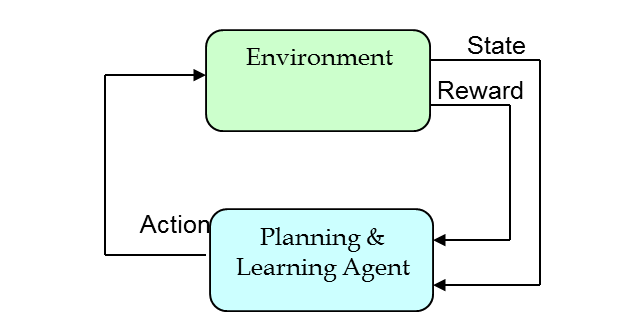
\includegraphics[width=0.5\textwidth]{lecture1_situated_agent}\\
  \caption{The situated agent}\label{fig:situated_agent}
  \end{centering}
\end{figure}

\begin{example}{\textbf{The Tetris player}}

Consider designing an AI player for the game of Tetris. The environment here would be the game simulator, and the environment state at a particular time corresponds to the game board at that time, and the shape of the new piece that just arrived. Upon observing a system state, the agent (the AI player) takes an action - it decides where on the board to position the new piece. Consequentially, if rows on the board were cleared, the agent receives a corresponding reward, and the the next system state is determined by the simulator.
\end{example}

\emph{Markov Decision Processes} (MDPs) are the standard model that allows to treat these planning and learning problems in a unified manner. An MDP describes a sequential decision problem, with the following properties:
\begin{itemize}
  \item A controlled dynamical system, with state-based dynamics. At each state some decision (or action) needs to be taken, and as a consequence the system moves to the next state.
  \item A reward function is associated with state-action pair, and the system performance is measured by the accumulated rewards.
  \item MDPs are especially suited to handle discrete problems (discrete state space, discrete action set, discrete time).
  \item MDPs allow to model in a natural way stochastic effects, and in particular stochastic system dynamics. We note that MDPs are currently the standard model for probabilistic planning in AI.
\end{itemize}

\subsection*{Challenges - what makes the planning problem hard?}
\begin{itemize}
  \item Lack of a global structure - most systems of interest do not have a simple global structure (such as that of a linear system). Therefore, planning needs to address each state (or group of states) in a distinct way.
  \item Large state-spaces: Many problems of interest have a huge number of states (recall the tetris example - how many board configurations are possible?), which makes exact solution impossible, even with the strongest algorithms.
        \emph{We note that models with a large number states are often the result of  combinatorial explosion in state vectors with a large number of components. This phenomenon is commonly known as the curse of dimensionality.}
  \item Large action-spaces: Some problems, especially in resource allocation, also exhibit large action-spaces, which present additional computational challenges.
  \item Stochastic effects - these are successfully handled within the MDP model, although they may add to the computational challenge.
  \item Uncertain or unknown environments -- which leads to the application of Reinforcement Learning techniques.
\end{itemize}

The computational challenge of complex problems (in particular, large state spaces) requires the use of approximation techniques for planning. This is an active research field, which is called Approximate Dynamic Programming (ADP) in our context. It is interesting to note that Reinforcement Learning techniques are often used as a means for planning in complex systems, even if the system dynamics is known.

The following diagram illustrates the relation and influence between the different disciplines involved.

  \begin{centering}
  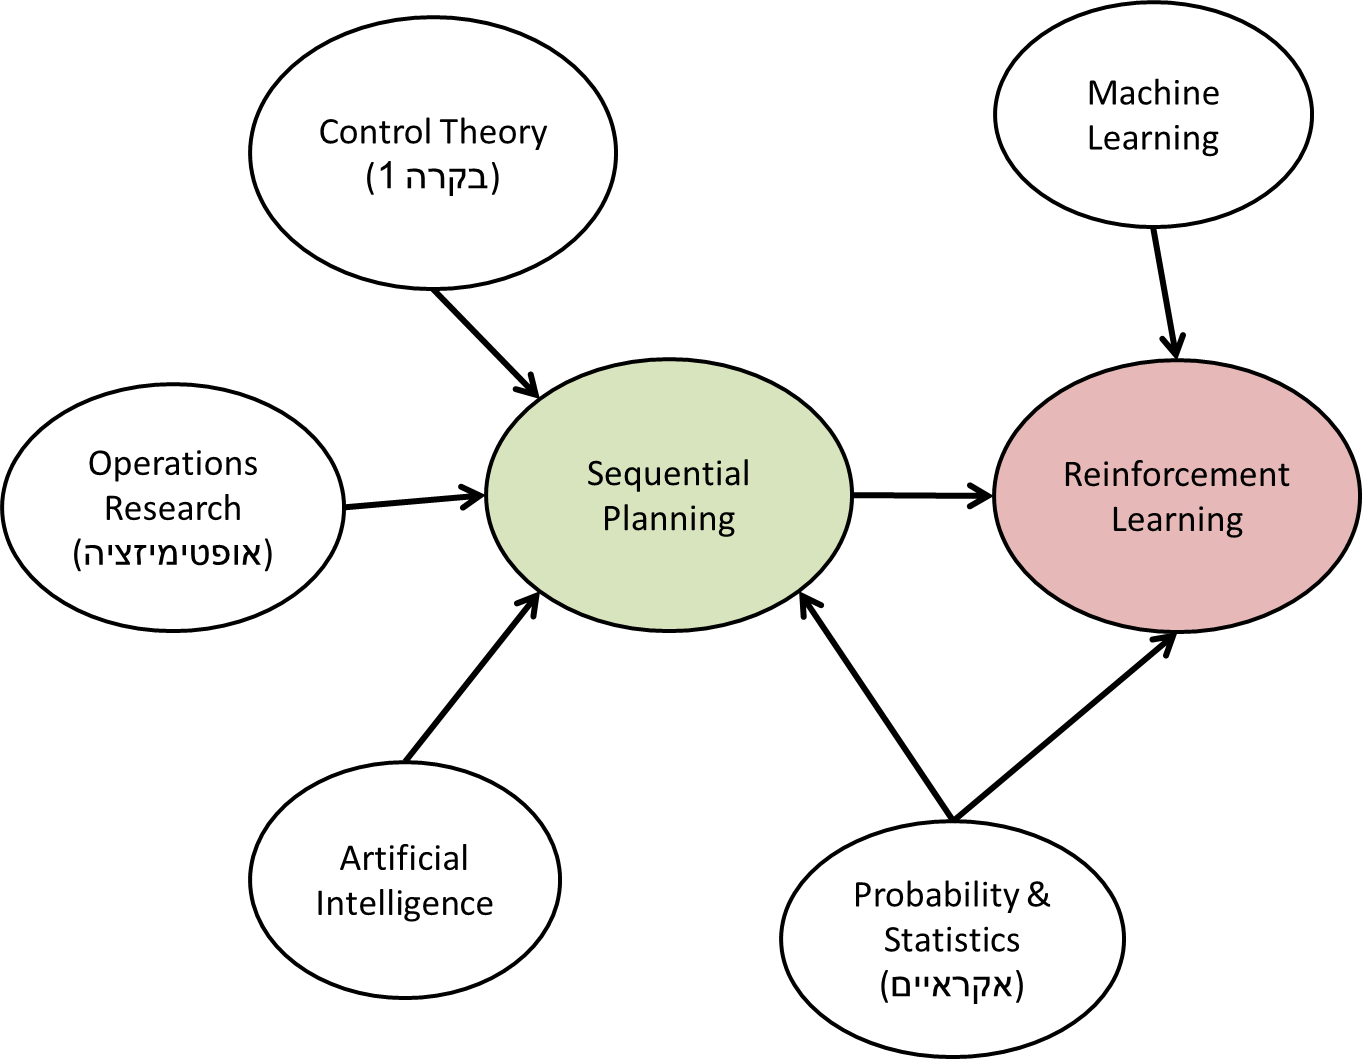
\includegraphics[width=0.7\textwidth]{lecture1_disciplines}\\
  \end{centering}

\section{Some Illustrative Planning Examples}
We next provide several examples that serve to illustrate the models involved. We start with planning examples.

\subsection{Shortest Path on a Graph}
Finding a shortest path between a source and destination nodes (or vertices) on a weighted graph is a generic problem with numerous applications, from routing in communication networks to trajectory planning, puzzle solving, and general AI planning. Essentially, Dynamic Programming based algorithms compute the distance from every node in the graph to the destination, spreading out from the destination until the source is reached. Specific algorithms for this problem include the Bellman-Ford algorithm, and Dijkstra's algorithm and its variants, such as A*.
This problem is widely discussed in courses on AI, and we will only briefly touch upon the main algorithms. We will also consider its stochastic generalization, the Stochastic Shortest Path problem.

\subsection{The Secretary Problem}
\paragraph{Problem setup:} We are interviewing $n$ candidates for a job. We know that the candidates are strictly ordered in quality from $1$ to $n$, but interview them in random order. Once we interview a candidate, his or her quality can be evaluated \emph{relative} to previously interviewed candidates. A candidate that is not hired during the interview cannot be recalled.
\paragraph{The planning problem:} Our goal is to find a rule for choosing a candidate, that will  maximize the chances of hiring the best one.

This problem and its generalizations have been widely studied in the operation research and computer science literature. It is an instance of a wider class of \emph{optimal stopping problems}.

\begin{exercise}
Let $B_t\sim \textrm{Bernoulli} $ i.i.d. for all $t=1,2,3,\dots$.
Consider the empirical average:
\begin{equation*}
    X_\tau = \frac{1}{\tau}\sum_{t=1}^{\tau} B_t.
\end{equation*}
where $\tau$ is a stopping time. The objective is to find a stopping rule for $\tau$ that maximizes $\mathbb E [X_\tau]$.
\begin{enumerate}
  \item Find a stopping rule that achieves $\mathbb E [X_\tau] \geq 0.75$
  \item (Hard!) What is the maximal $\mathbb E [X_\tau]$ that can be achieved?
\end{enumerate}
\end{exercise}

\subsection{Inventory Management}
\paragraph{System description:} Suppose we manage a single-item inventory system with daily orders. On the morning of each day $k$, we observe the current inventory ${x_k}$, and can order any quantity ${a_k} \ge 0$ of that item that arrives immediately. The daily demand for the item is denoted ${D_k}$. Thus, the number of items sold on each day $k$ is $\min \{ {D_k},{x_k} + {a_k}\} $, and the inventory at the end of the day is ${x_{k + 1}} = {[{x_k} + {a_k} - {D_k}]^ + }$. In this model we can determine the order $a_k$, whereas the demand $D_k$ is uncertain and is modeled as a random variable with known probability distribution. We assume that $D_k$ is a sequence of \emph{independent} random variables.

\paragraph{Cost structure:} Suppose that the cost for an order of $a_k$ is $J(a_k)$, a price $P$ is charged for each sold item, and a penalty $C({x_k} + {a_k} - {D_k})$ is incurred for over or under demand miss (where $C(y) \ge 0$ and  $C(0) = 0$).   Therefore, the net return (or reward) for day $k$ is \[{R_k} = P\,\min \{ {D_k},{x_k} + {a_k}\}  - J({a_k}) - C({x_k} + {a_k} - {D_k}).\]

The \emph{cumulative return} is the sum of daily returns over a given period, say $1$ to $K$.

\paragraph{The planning problem:} For each $k = 1, \ldots ,K$, we observe the current inventory $x_k$, and need to determine the amount $a_k$ to order next. The goal is to maximize the \emph{expected value} of the cumulative return over the given period:
\[E(\sum\nolimits_{k = 1}^K {{R_k}} )\; \to \;\min \]

\begin{remark}: A common policy in inventory management is the $(s,S)$ replenishment policy: whenever the inventory $x$ drops below $s$, order $S-x$ items. This policy can be shown to be optimal under appropriate assumptions on the cost.
\end{remark}
\begin{exercise} For the single-stage problem $(K=1)$  with $R=0$, $J\equiv0$, $C(y)=y^2$, show that a $(s,S)$ policy is optimal (with $s=S$).
\end{exercise}

\subsection{Admission control to a queueing system}
\paragraph{System description:} Consider a single-server queue, to which jobs (or customers) arrive sequentially. Each job has a service demand (in time unit of service) that is represented by a random variable with known distribution. The arrival process is, say, Poisson with rate $\lambda$.  The system manager can deny admission to an arriving job.

\paragraph{Cost structure:} Suppose that the system incurs a penalty of $C$ per unit time for each job waiting in the queue, and a reward $R$ for each customer served. We wish to minimize the expected cumulative cost over a period of time.

\paragraph{The planning problem:} Suppose a job arrives when the queue size is $x\geq0$. Should it be admitted or denied entry?
This problem represents a basic example of \emph{queueing control problems}. A wide range of computer, communication, and service systems can be represented by networks of queues (waiting lines) and servers. Efficient operation of these systems gives rise to a wide range of dynamic optimization problems. These include, among others, job admission control, job routing, server and job scheduling, and control of service rates.

\subsection{Stochastic scheduling}
\paragraph{System description: } Suppose we have a single server that caters to $n$ classes of jobs, one job at a time. Here the server may be human, a router in a communication network, a CPU in a computer system, etc. Jobs of class $i$ arrive as a Poisson process with rate $\lambda_i$, and each requires a service duration $D_i$ (which could be random -- for example, an exponentially-distributed random variable with expected value $\mu _i^{ - 1}$).

\paragraph{Cost structure:} Jobs of class $i$ incur a waiting cost  $C_i$ per unit time of waiting for service, and a reward $R_i$ for completing service.

\paragraph{The planning problem:} Suppose that the server becomes available at an instance $t$, and sees the state vector $X(t) = ({x_1}(t), \ldots ,{x_n}(t))$, where $x_i$ is the number of class $i$ jobs waiting for service. Which job class should the server attend next?

\section{Some Illustrative Learning Examples}
The following examples address the learning problem.

\subsection{The Multi-Armed Bandit (MAB) problem}
This is an important problem in statistics and machine learning. The exotic name derives from casino-like slot machines, which are also known as "single-armed bandits".
Suppose we are faced with $N$ different arms (slot machines), which may have different win probabilities (for simplicity assume 0-1 results, with obvious generalizations). These probabilities are not known to us.
There are two different goals in this problem:
\begin{enumerate}
  \item To identify the best arm (pure exploration).
  \item To maximize our gains over a large time horizon (exploration vs. exploitation).
\end{enumerate}

This model, under the second objective, presents in its purest form the \textbf{exploration vs. exploitation dilemma}, which is fundamental in Reinforcement Learning: While each arm may be optimal and should be sufficiently tried out, we should also focus at some point on the arm that seems to be the best. This tradeoff must be addressed by an appropriate  \emph{exploration strategy}.

We note that this problem can be considered as a special case of the MDP model, with a single state (i.e., static environment). Its original motivation was related to experimental drug (medicine) administration. Its current popularity in Machine Learning owes to recent on-line application such as ad posting: choosing the right class of ads to post in a given space or context to maximize revenue (or "click" count).

\subsection{Learning to Play Chess / Backgammon}
Current AI programs for chess playing essentially rely on extensive search in the game tree, starting from the current board position. That search is aided by an evaluation function (the \emph{heuristic}, or \emph{value function}), which provides a numerical value to each board position that estimates its strength (say, the likelihood of a win).

Suppose for simplicity that the opponent's playing strategy is known, so that the problem reduces to a single-player planning problem. The problem, of course, is huge number of states (board positions), which rules out an exact and complete solution. Therefore, partial solutions guided by heuristic and empirical rules must be used.

Machine learning offers a set of tools to improve the performance of a given AI player, by data-based tuning key parameter of the algorithm. Such improvements are often imperative for achieving state-of-the-art performance. Specific topics in which RL techniques have been successfully applied include:

\begin{itemize}
  \item Value function learning (by self-play and record analysis).
  \item Powerful heuristics for guiding the tree search.
\end{itemize}
These techniques have been applied in the games of Backgammon, Chess, and recently Go and Poker.

\subsection{Skill Learning in Robotics}
Suppose we wish to program a robot to juggle a ball on a racket, or to walk efficiently. We can start by programming the robot as best we can, but in most cases we will not be able to obtain fully efficient operation that way, and many "fine tunings" will be required.  One of the major approaches for improvement is to equip the robot with learning capabilities, so that it can improve its performance over time.
We can distinguish here between two learning goals:
\begin{enumerate}
\item[a.] Short term learning, or adaptivity - adapting to changing environment conditions (such as the weight of the ball, wind, etc.).
\item[b.] Skill learning - acquiring and improving the basic capability to perform certain motions or tasks in an efficient manner.
\end{enumerate}

A major Reinforcement Learning approach to these learning problems is a set of methods called \emph{direct policy search}. Here the required task or motion is parameterized by a vector of continuous parameters, which are tuned by simulation or during actual operation using gradient-based methods.  We will touch upon this important topic towards the end of the course.

\section{Mathematical Tools}
We briefly mention the main mathematical tools that will be used throughout the course.
\begin{enumerate}
  \item Concentration inequalities
  \item MDPs - dynamic programming
  \item Optimization - algorithms and theory
  \item Generalization and risk (PAC)
  \item Approximation theory
  \item Convergence of stochastic processes
\end{enumerate}

%\end{document}



\chapter{Deterministic Decision Processes}
%\documentclass[11pt]{article}
%\usepackage{geometry}                % See geometry.pdf to learn the layout options. There are lots.
%\geometry{letterpaper}                   % ... or a4paper or a5paper or ...
%%\geometry{landscape}                % Activate for for rotated page geometry
%%\usepackage[parfill]{parskip}    % Activate to begin paragraphs with an empty line rather than an indent
%\usepackage{graphicx}
%\usepackage{amssymb}
%\usepackage{epstopdf}
%\usepackage{amsfonts}
%\usepackage{amsthm}
%\usepackage{amsmath}
%\usepackage{tikz}
%\usepackage{algorithm2e}
%\usepackage{url}
%\usepackage{comment}
%
%\newcommand{\mdp}{\mathcal{M}}
%\newcommand{\Mdp}{\mathcal{M}}
%\newcommand{\Agent}{\mathcal{G}}
%\newcommand{\env}{\mdp}
%\newcommand{\Env}{\mdp}
%\newcommand{\Actions}{\mathcal{A}}
%\newcommand{\action}{a}
%\newcommand{\actionp}{a^{\prime}}
%\newcommand{\actionpp}{a^{\prime\prime}}
%\newcommand{\States}{\mathcal{S}}
%\newcommand{\state}{s}
%\newcommand{\statep}{\state^{\prime}}
%\newcommand{\statepp}{\state^{\prime\prime}}
%\newcommand{\eststate}{x}
%
%\newcommand{\obs}{o}
%\newcommand{\Obs}{\mathcal{O}}
%\newcommand{\reward}{r}
%\newcommand{\terminalreward}{r^T}
%\newcommand{\rew}{\reward}
%\newcommand{\Rewards}{\mathcal{R}}
%\newcommand{\history}{h}
%\newcommand{\histories}{\mathcal{H}}
%\newcommand{\Histories}{\mathcal{H}}
%\newcommand{\Trans}{T}
%\newcommand{\Horizon}{t_f}
%\newcommand{\TUtility}{U_T}
%\newcommand{\Utility}{U_{\gamma}}
%\newcommand{\AUtility}{U_A}
%\newcommand{\TValue}{J}
%\newcommand{\TAValue}{K}
%\newcommand{\Value}{V}
%\newcommand{\hatValue}{{\widehat{V}}}
%\newcommand{\AValue}{Q}
%\newcommand{\hatAValue}{{\widehat{Q}}}
%\newcommand{\AvgRValue}{\rho}
%\newcommand{\hatAvgRValue}{{\widehat{\rho}}}
%\newcommand{\RelValue}{W}
%\newcommand{\hatRelValue}{{\widehat{W}}}
%
%\newcommand{\stateestfunction}{f_{su}}
%\newcommand{\stateobsfunction}{f_{so}}
%\newcommand{\statetransfunction}{f_{ss}}
%\newcommand{\rewfunction}{f_r}
%\newcommand{\field}[1]{\mathbb{#1}}
%\newcommand{\Reals}{\field{R}}
%%\newcommand{\eqref}[1]{(\ref{#1})}
%\newcommand{\policy}{\pi}
%\newcommand{\hatpolicy}{{\widehat{\pi}}}
%\newcommand{\Policies}{\Pi}
%\newcommand{\nspolicy}{\mu}
%
%\newcommand{\union}{\ensuremath{\bigcup}}
%\newcommand{\comps}{\ensuremath{\mathbb{C}}}
%\newcommand{\reals}{\ensuremath{\mathbb{R}}}
%\newcommand{\Var}{\ensuremath{\mathrm{Var}}}
%\newcommand{\var}{\ensuremath{\mathrm{Var}}}
%\newcommand{\E}{\ensuremath{\mathbb{E}}}
%\renewcommand{\P}{\ensuremath{\mathbb{P}}}
%\newcommand{\R}{\ensuremath{\mathbb{R}}}
%\newcommand{\Z}{\ensuremath{\mathbb{Z}}}
%
%\newcommand{\mixtime}{\tau}
%\newcommand{\epshorizon}{\tau}
%
%\def\argmax{\operatornamewithlimits{arg\,max}}
%\def\argmin{\operatornamewithlimits{arg\,min}}
%
%\newcommand{\bydef}{\stackrel{\bigtriangleup}{=}}
%\newcommand\defeq{\stackrel{\mathrm{def}}{=}}
%\newcommand{\half}{\frac{1}{2}}
%
%\DeclareGraphicsRule{.tif}{png}{.png}{`convert #1 `dirname #1`/`basename #1 .tif`.png}
%
%\newtheorem{proposition}{Proposition}
%\newtheorem{corollary}{Corollary}
%\newtheorem{assumption}{Assumption}
%\newtheorem{lemma}{Lemma}
%\newtheorem{definition}{Definition}
%\newtheorem{theorem}{Theorem}
%\newtheorem{example}{Example}
%\newtheorem{exercise}{Exercise}
%\newtheorem{remark}{Remark}
%\newtheorem{algorithm_}{Algorithm}
%
%\title{Lecture 2 -- Deterministic Decision Processes}
%\date{}                                           % Activate to display a given date or no date
%
%\begin{document}
%\maketitle

In this chapter we introduce the dynamic system viewpoint of the optimal planning problem. We restrict the discussion here to deterministic (rather than stochastic) systems, and consider the finite-horizon decision problem and its recursive solution via finite-horizon Dynamic Programming.

\section{Discrete Dynamic Systems}
We consider a discrete-time dynamic system, of the form:
\[{x_{k + 1}} = {f_k}({x_k},{u_k}),\quad k = 0,1,2, \ldots ,N - 1\]
where
\begin{itemize}
  \item $k$ is the time index.
  \item ${x_k} \in {X_k}$ is the state variable at time $k$, and $X_k$ is the set of possible states at time $k$.
  \item ${u_k} \in {U_k}$  is the control variable at time $k$, and $U_k$ is the set of possible control values (or actions) at time $k$.
  \item ${f_k}:{X_k} \times {U_k} \to {X_{k + 1}}$ is the state transition function, which defines the \emph{state dynamics} at time $k$.
  \item $N>0$ is the \emph{time horizon} of the system.  It can be finite or infinite.
\end{itemize}
 	
\begin{remark}
 	More generally, the set $U_k$ of available actions may depend on the state at time $k$, namely: ${u_k} \in {U_k}({x_k}) \subset {U_k}$.
\end{remark}
\begin{remark}
 	The system is in general time-varying. It is called \emph{time invariant} if ${f_k},{X_k},{U_k}$ do not depend on the time $k$. In that case we write
\[{x_{k + 1}} = f({x_k},{u_k}),\quad k = 0,1,2, \ldots ,N - 1;\quad {x_k} \in X,\;{u_k} \in U({x_k}).\]
\end{remark}
\begin{remark}
 	The state dynamics may be augmented by an output equation:
\[{y_k} = {h_k}({x_k},{u_k})\]
\end{remark}
where  $y_k$ is the system output, or the observation. In most of this course we  implicitly assume that $y_k=x_k$, namely, the current state $x_k$ is fully observed.

\begin{example}{\textbf{Linear Systems}}

The best known example of a dynamic system is that of a linear time-invariant system, where:
\[{x_{k + 1}} = A{x_k} + B{u_k}\]
with ${x_k} \in \R^n$, $u_k \in \R^m$. Here the state and action spaces are evidently continuous (as opposed to discrete).
\end{example}

\begin{example}{\textbf{Finite models}}

Our emphasis here will be on \emph{finite state and action} models. A finite state space contains a finite number of points: ${X_k} = \{ 1,2, \ldots ,{n_k}\} $. Similarly, a finite action space implies a finite number of control values at each stage:
\[{U_k}(x) = \{ 1,2, \ldots ,{m_k}(x)\} ,\;\;x \in {X_k}\]
\end{example}

\paragraph{Notation for finite models:}  When the state and action spaces are finite, it is common to denote the state by ${s_k}$ (instead of ${x_k}$) and the actions by ${a_k}$ (instead of ${u_k}$). That is, the system equations are written as:
${s_{k + 1}} = {f_k}({s_k},{a_k}),\quad k = 0,1,2, \ldots ,N - 1$
with ${s_k} \in {S_k}$, ${a_k} \in {A_k}({s_k}) \subset {A_k}$.  \textbf{We will adhere to that notation in the following}.


\paragraph{Graphical description:} Finite models (over finite time horizons) can be represented by a corresponding decision graph:

\begin{centering}
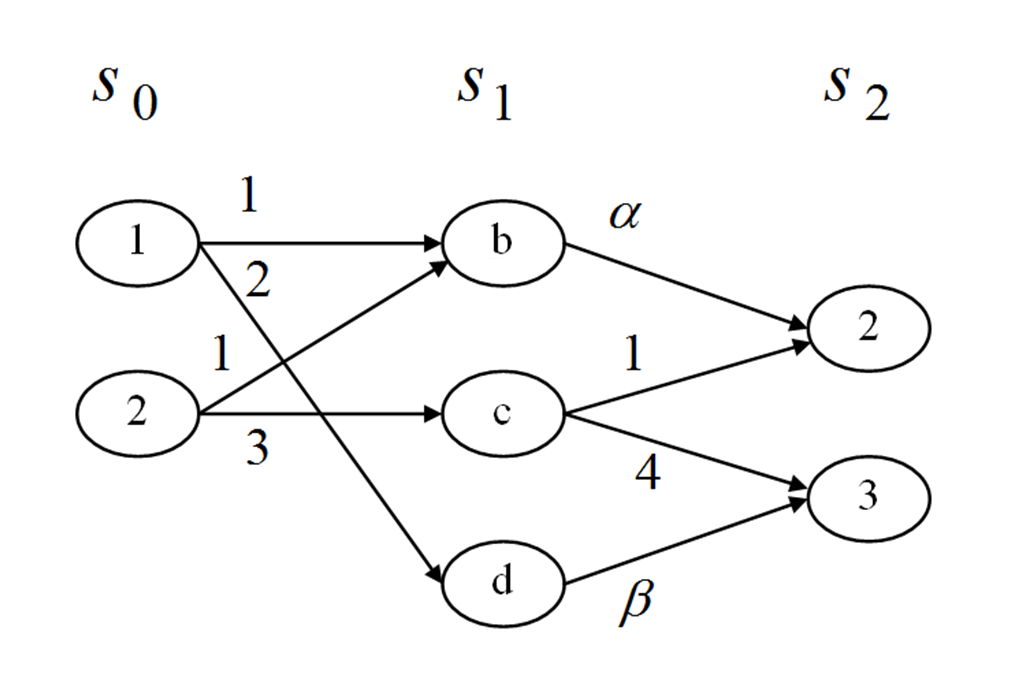
\includegraphics[width=0.5\textwidth]{lecture2_decision_graph}\\
\end{centering}

Here:
\begin{itemize}
  \item $N = 2$, ${S_0} = \{ 1,2\} ,\;{S_1} = \{ b,c,d\} ,\;{S_2} = \{ 2,3\} $,
  \item ${A_0}(1) = \{ 1,2\} $, ${A_0}(2) = \{ 1,3\} $, ${A_1}(b) = \{ \alpha \} $, ${A_1}(c) = \{ 1,4\} $, ${A_1}(d) = \{ \beta \} $
  \item ${f_0}(1,1) = b,\;{f_0}(1,2) = d,\;{f_0}(2,1) = b,\;{f_0}(2,3) = c$, ${f_1}(b,\alpha ) = 2$, etc.
\end{itemize}

\begin{definition}{\textbf{Feasible Path}} \\
A feasible path for the specified system is a sequence $({s_0},{a_0}, \ldots ,{s_{N - 1}},{a_{N - 1}},{s_N})$ of states and actions, such that ${a_k} \in {A_k}({s_k})$ and ${s_{k + 1}} = {f_k}({s_k},{a_k})$.

\vspace{10pt}
\begin{centering}
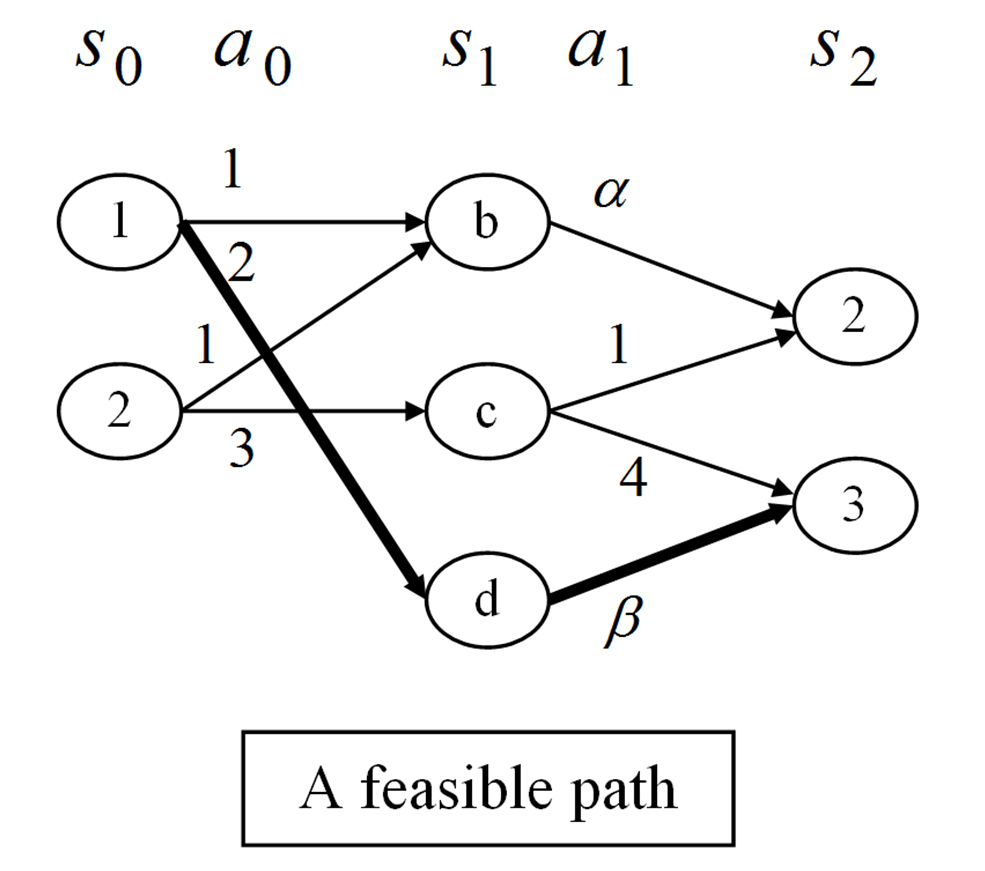
\includegraphics[width=0.4\textwidth]{lecture2_feasible_path}\\
\end{centering}
\end{definition}

\section{The Finite Horizon Decision Problem}

We proceed to define our first and simplest planning problem. For that we need to specify a \emph{performance objective} for our model, and the notion of \emph{control policies}.

\subsection{Costs and Rewards}

\paragraph{The cumulative cost:}  Let ${h_N} = ({s_0},{a_0}, \ldots ,{s_{N - 1}},{a_{N - 1}},{s_N})$ denote an $N$-stage path for the system..  To each feasible path ${h_N}$ we wish to assign some cost ${C_N} = {C_N}({h_N})$.

The standard definition of the cost ${C_N}$ is through the following \emph{cumulative cost functional}:
\[{C_N}({h_N}) = \sum\limits_{k = 0}^{N - 1} {{c_k}({s_k},{a_k}) + {c_N}({s_N})} \]

Here:
 	\begin{itemize}
    \item ${c_k}({s_k},{a_k})$ is the \emph{instantaneous}  cost or \emph{single-stage }cost at stage $k$, and ${c_k}$ is the instantaneous cost function.
    \item ${c_N}({s_N})$ is the \emph{terminal} cost, and ${c_N}$ is the terminal cost function.
  \end{itemize}

\paragraph{Note:}
\begin{itemize}
  \item The cost functional defined above is \emph{additive} in time. Other cost functionals are possible, for example the max cost, but additive cost is by far the most common and useful.
  \item We shall refer to ${C_N}$ as the \emph{cumulative $N$-stage cost}, or just the \emph{cumulative cost}.
\end{itemize}

Our objective is to \emph{minimize} the cumulative cost ${C_N}$, by a proper choice of actions. We will define that goal more formally below.

\paragraph{Cost versus reward formulation: }It is often more natural to consider \emph{maximizing} reward rather than minimizing cost.  In that case, we define the cumulative $N$-stage return function:
$${R_N}({h_N}) = \sum\limits_{k = 0}^{N - 1} {{r_k}({s_k},{a_k}) + {r_N}({s_N})} $$
Here and ${r_k}$ is the running reward, and  ${r_N}$ is the terminal reward.
Clearly, minimizing ${C_N}$ is equivalent to maximizing ${R_N}$, if we set:
$${r_k}(s,a) =  - {c_k}(s,a) \text{ and }{r_N}(s) =  - {c_N}(s).$$


\subsection{Optimal Paths}

Our first planning problem is the following \emph{Path Optimization Problem}:
\begin{itemize}
  \item For a given initial state ${s_0}$, find a feasible path ${h_N} = ({s_0},{a_0}, \ldots ,{s_{N - 1}},{a_{N - 1}},{s_N})$ that minimizes the cost functional ${C_N}({h_N})$, over all feasible paths ${h_N}$.
\end{itemize}

Such a path is called an \emph{optimal path} from ${s_0}$.

A more general notion than a path is that of a \emph{control policy}, that specifies the action to be taken at each state. Control policies will play an important role in our Dynamic Programming algorithms, and are defined next.

\subsection{Control Policies}

\begin{definition} A control policy, denoted $\pi $, specifies for each state a unique action to be taken at this state. Specifically, a control policy  $\pi $ is a sequence $\pi  = ({\pi _0}, \ldots ,{\pi _{N - 1}})$ of decision functions, where
${\pi _k}:{S_k} \to {A_k}$,    and  ${\pi _k}(s) \in {A_k}(s)$.
The action to be taken at time $k$ in state ${s_k}$ is given as
${a_k} = {\pi _k}({s_k})$
\end{definition}

\paragraph{Classes of control policies}
Observe that we allow the function ${\pi _k}$ policy to depend on the time $k$. Such time-dependent policies are also called \emph{non-stationary}. On the other hand, we confine ourselves here to policies that are:
\begin{itemize}
  \item \textbf{Markovian}: The action ${a_k}$ is a function of the current state ${s_k}$ only, and not on previous states and actions. Non-Markovian policies: also called history-dependent policies, will be extensively used in the learning part of the course.
  \item \textbf{Deterministic}: More general policies may use randomization in the selection of actions. Such randomized policies are also used in learning algorithms, as well as in game problems.
\end{itemize}

\paragraph{Control policies and paths:} As mentioned, a control policy specifies an action for each state, whereas a path specifies an action only for states along the path. This distinction is illustrated in the following figure.

\begin{centering}
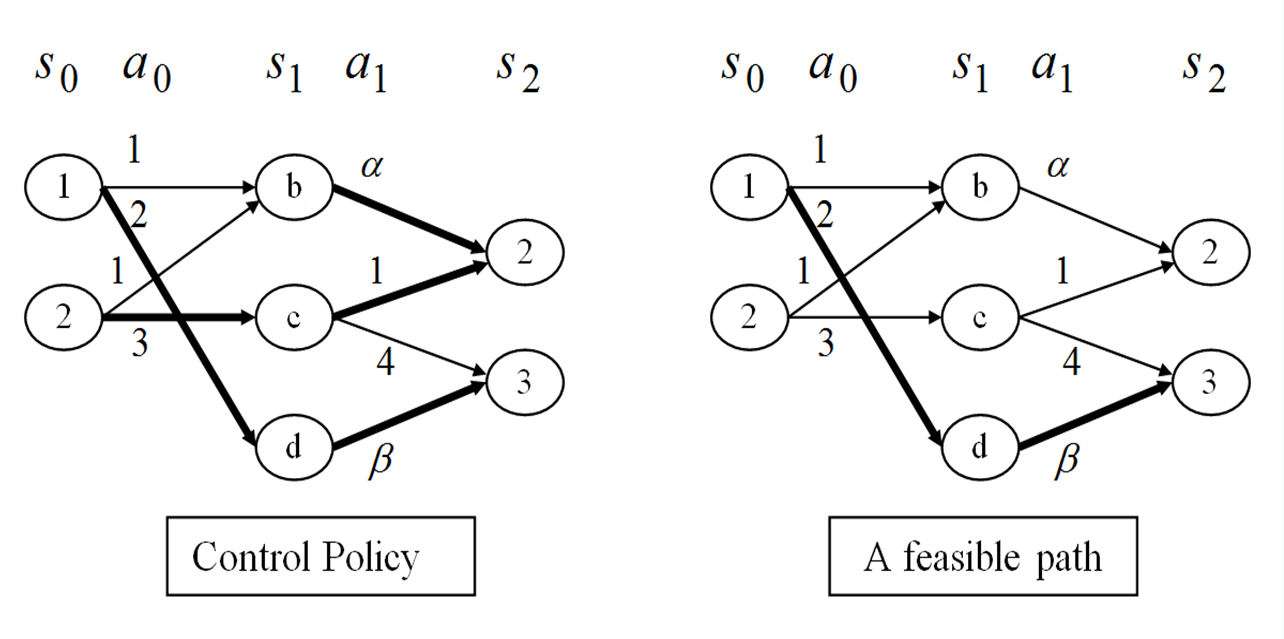
\includegraphics[width=0.8\textwidth]{lecture2_policy_path}\\
\end{centering}

\paragraph{Induced Path:} A control policy $\pi $, together with an initial state ${s_0}$, specify a feasible path ${h_N} = ({s_0},{a_0}, \ldots ,{s_{N - 1}},{a_{N - 1}},{s_N})$. This path may be computed recursively using ${a_k} = {\pi _k}({s_k})$ and ${s_{k + 1}} = {f_k}({s_k},{a_k})$, for $k = 0,1, \ldots ,N - 1$.

\begin{remark} Suppose that for each state ${s_k}$, each action ${a_k} \in {A_k}({s_k})$ leads to a different state ${s_{k + 1}}$ (i.e., at most one edge connects any two states). We can then identify each action ${a_k} \in {A_k}(s)$ with the next state ${s_{k + 1}} = {f_k}(s,{a_k})$ it induces. In that case a path may be uniquely specified by the state sequence $({s_0},{s_1}, \ldots ,{s_N})$.
\end{remark}

\subsection{Optimal Control Policies}

\begin{definition} A control policy $\pi $ is called \textbf{optimal} if, for each initial state ${s_0}$, it induces an optimal path ${h_N}$ from ${s_0}$.
\end{definition}

An alternative definition can be given in terms of policies only. For that purpose, let ${h_N}(\pi ;{s_0})$ denote the path induced by the policy $\pi $ from ${s_0}$.  For a given return  functional ${R_N}({h_N})$, denote
${R_N}(\pi ;{s_0}) = {R_N}({h_N}(\pi ;{s_0}))$
That is, ${R_N}(\pi ;{s_0})$ is the cumulative return for the path induced by by $\pi $ from ${s_0}$.

\begin{definition} A control policy $\pi $ is called optimal if, for each initial state ${s_0}$, it holds that ${R_N}(\pi ;{s_0}) \ge {R_N}(\tilde \pi ;{s_0})$
for any other policy $\tilde \pi $.
\end{definition}

Equivalence of the two definitions can be easily established (exercise). An optimal policy is often denoted by ${\pi ^*}$.

\vspace{10pt}
\fbox{\begin{minipage}{0.9\textwidth}
\textbf{The standard finite-horizon planning problem:}  Find a control policy $\pi $ for the $N$-stage decision problem with the cumulative return (or cost) function.
\end{minipage}}


\normalsize
\paragraph{The naive approach to finding an optimal policy:}  For finite models (i.e., finite state and action spaces), the number of feasible paths (or control policies) is finite.  It is therefore possible, in principle, to enumerate all N-stage paths, compute the cumulative return for each one, and choose the one which gives the largest return.
Let us evaluate the number of different paths and control policies.
Suppose for simplicity that number of states at each stage is the same: $|{X_k}| = n$, and similarly the number of actions at each state is the same: $|{A_k}(x)| = m$ (with $m \le n$) . The number of feasible N-stage paths for each initial state is seen to be ${m^N}$. The number of different policies is ${m^{nN}}$.
For example, for a fairly small problem with $N = n = m = 10$, we obtain ${10^{10}}$ paths for each initial state (and ${10^{11}}$ overall), and ${10^{100}}$ control policies. Clearly it is not possible to enumerate them all.

Fortunately, Dynamic Programming offers a drastic simplification of the computational complexity for this problem.

\section{Finite Horizon Dynamic Programming}

The Dynamic Programming (DP) algorithm breaks down the $N$-stage decision problem into $N$ sequential single-stage optimization problems. This results in dramatic improvement in computation efficiency.

The DP technique for dynamic systems is based on a general observation called Bellman's Principle of Optimality. Essentially it states the following (for deterministic problems):
\begin{itemize}
  \item \textbf{Any sub-path of an optimal path is itself an optimal path between its end point.}
\end{itemize}

Applying this principle recursively from the last stage backward, obtains the (backward) Dynamic Programming algorithm. Let us first illustrate the idea with following example.

\begin{example} Shortest path on a decision graph:  Suppose we wish to find the shortest path (minimum cost path) from the initial node in $N$ steps.

\begin{centering}
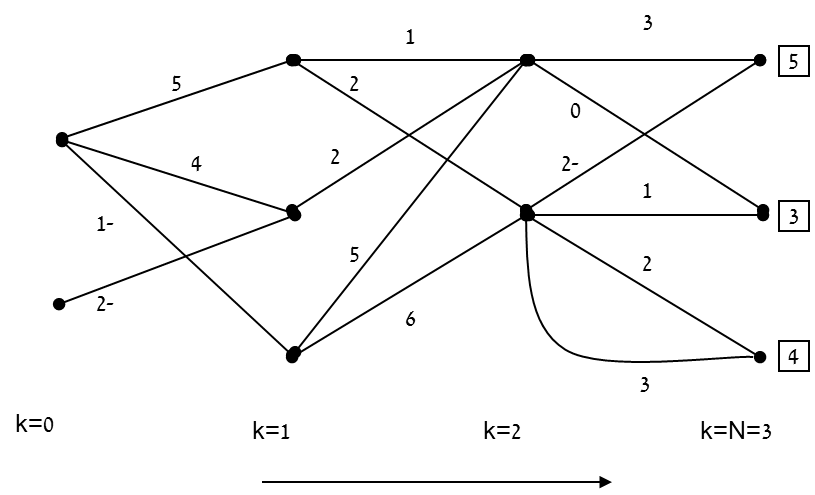
\includegraphics[width=0.8\textwidth]{lecture2_DP}
\end{centering}
\\
The boxed values are the terminal costs at stage $N$, the other number are the link costs.
Using backward recursion, we may obtain that the minimal path costs from the two initial states are 7 and 3, as well as the optimal paths and an optimal policy.

\end{example}

We can now describe the DP algorithm. Recall that we consider the dynamic system
$${s_{k + 1}} = {f_k}({s_k},{a_k}),\quad k = 0,1,2, \ldots ,N - 1$$
$${s_k} \in {S_k},\quad {a_k} \in {A_k}({s_k})$$
and we wish to maximize the cumulative return:
$${R_N} = \sum\limits_{k = 0}^{N - 1} {{r_k}({s_k},{a_k}) + {r_N}({s_N})} $$
The DP algorithm computes recursively a set of \textbf{value functions} $V_k^{}:{S_k} \to \R$ , where $V_k^{}({s_k})$ is the value of an optimal sub-path ${h_{k:N}} = ({s_k},{a_k}, \ldots ,{s_N})$ that starts at ${s_k}$.

\begin{algorithm_}
\textbf{Finite-horizon Dynamic Programming}
\begin{enumerate}
  \item Initialize the value function:   $V_N^{}(s) = {r_N}(s)$,  $s \in {S_N}$.
  \item Backward recursion:  For $k = N - 1, \ldots ,0$, compute
\[V_k^{}(s) = \mathop {\max }\limits_{a \in {A_k}} \left\{ {{r_k}(s,a) + V_{k + 1}^{}({f_k}(s,a))} \right\},\quad     s \in {S_k}.\]
  \item Optimal policy: Choose any control policy $\pi  = ({\pi _k})$ that satisfies:
\[\pi _k^{}(s) \in \mathop {\arg \max }\limits_{a \in {A_k}} \left\{ {{r_k}(s,a) + V_{k + 1}^{}({f_k}(s,a))} \right\},\quad      k = 0, \ldots ,N - 1.\]
\end{enumerate}
\end{algorithm_}

\begin{proposition}
The following holds for finite-horizon dynamic programming:
\begin{enumerate}
  \item The control policy $\pi $ computed above is an optimal control policy for the $N$-stage decision problem.
  \item $V_0^{}(s)$ is the optimal N-stage return from initial state ${s_0} = s$:
\[{V_0}(s) = \mathop {\max }\limits_\pi  {R_N}(\pi ;s),\;\quad \forall s \in {S_0}.\]
\end{enumerate}
\end{proposition}

We will provide a proof of this result in a later lecture, for the more general stochastic MDP model. For the time being, let us make the following observations:
\begin{enumerate}
  \item The algorithm involves visits each state exactly once, proceeding backward in time. For each time instant (or stage) $k$, the value function ${V_k}(s)$ is computed for all states $s \in {S_k}$ before proceeding to stage $k - 1$.
  \item The recursive equation in part 2 of the algorithm, along with similar equations in the theory of DP, is called \textbf{Bellman's equation}.
  \item Computational complexity: There is a total of $nN$ states (excluding the final one), and in each we need $m$ computations. Hence, the number of required calculations is $mnN$.
For the example above with $m = n = N = 10$, we need $O({10^3})$ calculations.
  \item A similar algorithm that proceeds forward in time (from $k = 0$ to $k = N$) can be devised. We note that this will not be possible for stochastic systems (i.e., the stochastic MDP model).
  \item The celebrated \textbf{Viterbi algorithm} is an important instance of finite-horizon DP. The algorithm essentially finds the most likely sequence of states in a Markov chain $({s_k})$ that is partially (or noisily) observed.
The algorithm was introduced in 1967 for decoding convolution codes over noisy digital communication links. It has found extensive applications in communications, and is a basic computational tool in Hidden Markov Models (HMMs), a popular statistical model that is used extensively in speech recognition and bioinformatics, among other areas.
\end{enumerate}

\paragraph{Historical Notes:}
\begin{itemize}
  \item Dynamic Programming was popularized in the 1950's and 1960's by \textbf{Richard Bellman} (1920-1984), an American mathematician (of Jewish descent). Bellman, who coined the term Dynamic Programming, formulated the general theory and proposed numerous applications in control and operations research.
  \item \textbf{Andrew Viterbi} (born 1935) is an American professor of electric engineer, a pioneer in the field of digital communications, and co-founder of Qualcomm Inc. (together with Irwin Jacobs). He has had close ties with the Technion, and has made many contributions to our department.
\end{itemize}




%\end{document}



\chapter{Other Deterministic Dynamic Programming Algorithms}
Dynamic Programming (DP) can be used to solve various computational problems that do not fall into the dynamic system framework which is our focus in this course. In this lecture we will briefly consider DP solutions to several such problems. Our treatment will be brief and informal.

This lecture is partly based on Chapter 15 of the textbook:

\textbf{T. Cormen, C. Leliserson, R. Rivest and C. Stein, Introduction to Algorithms, 2nd ed., MIT Press, 2001}.

Some of the problems below are nicely explained in
\url{http://people.cs.clemson.edu/~bcdean/dp_practice/}

\section{Specific Computational Problems }

Dynamic Programming can be seen as a general approach for solving large computation problems by breaking them down into nested subproblems, and recursively combining the solutions to these subproblems. A key point is to organize the computation such that each subproblem is solved only once.

In many of these problems the recursive structure is not evident or unique, and its proper identification is part of the solution.

\subsection{Maximum contiguous sum}
\paragraph{Given: }  A (long) sequence of $n$ real numbers ${a_1},{a_2}, \ldots ,{a_n}$ (both positive and negative).
\paragraph{Goal:}   Find  ${V^*} = \mathop {\max }\limits_{1 \le i \le j \le n} \;\,\sum\limits_{\ell  = i}^j {{a_\ell }} .$

An exhaustive search needs to examine $O({n^2})$ sums. Can this be done more efficiently?

\paragraph{DP Solution in linear time:}
Let   ${M_k} = \mathop {\max }\limits_{1 \le i \le k} \sum\limits_{\ell  = i}^k {{a_\ell }} $  denote the maximal sum over all contiguous subsequences that end exactly at ${a_k}$.

Then $${M_1} = {a_1},$$ and
$${M_k} = \max \{ {M_{k - 1}} + {a_k},\,\,{a_k}\} .$$
We may compute ${M_k}$ recursively for $k = 2:n$. The required solution is given by
$${V^*} = \max \{ {M_1},{M_2}, \ldots ,{M_n}\} ,$$
This procedure requires only $O(n)$ calculations, i.e., linear time.

\paragraph{Note:}  The above computation gives the value of the maximal sum. If we need to know the range of elements that contribute to that sum, we need to keep track of the indices that maximized the various steps in the recursion.

\subsection{Longest increasing subsequence}

\paragraph{Given:}   A sequence of $n$ real numbers ${a_1},{a_2}, \ldots ,{a_n}$.
\paragraph{Goal:}   Find the longest strictly increasing subsequence (not necessarily contiguous).
E.g, for the sequence $(3,1,5,3,4)$, the solution is $(1,3,4)$.
Observe that the number of subsequences is ${2^n}$, therefore an exhaustive search is inefficient.

\paragraph{DP solution:}
Define  ${L_j} = $ {longest strictly increasing subsequence ending at position $j$}.
Then $${L_1} = 1,$$
$${L_j} = \max \{ {L_i}\,\;:\;\;i < j,\;\,{a_i} < {a_j}\}  + 1,\quad   j > 1$$
and the size of the longest subsequence is $L^* = {\max _{1 \le j \le n}}({L_j}).$
\\
Computing ${L_j}$ recursively for $j = 1:n$ gives the result with a running time\footnote{We note that this can be further improved to $O(n\log n)$. See Chapter 15 of
the `Introduction to Algorithms' textbook for more details.} of $O({n^2})$.


\subsection{An integer knapsack problem}

\paragraph{Given:}   A knapsack (bag) of capacity $C > 0$, and a set of $n$ items with respective sizes ${S_1}, \ldots ,{S_n}$ and values (worth) ${V_1}, \ldots ,{V_n}$. The sizes are positive and integer-valued.
\paragraph{Goal:}  Fill the knapsack to maximize the total value. That is, find the subset $A \subset \{ 1, \ldots ,n\} $ of items that maximize \[\sum\nolimits_{i \in A} {{V_i}} ,\] subject to  \[\sum\nolimits_{i \in A} {{S_i}}  \le C.\]

Note that the number of item subsets is ${2^n}$.

\paragraph{DP solution:}
Let $M(i,k) = $ maximal value for filling exactly capacity $k$ with items from the set $1:i$.
If the capacity $k$ cannot be matched by any such subset, set $M(i,k) =  - \infty $.
Also set $M(0,0) = 0$, and  $M(0,k) =  - \infty $ for $k \ge 1$.  Then
$$M(i,k) = \max \{ M(i - 1,k)\,,\,\,M(i - 1,k - {S_i}) + {V_i}\} ,$$
which can be computed recursively for $i = 1:n$,  $k = 1:C$. The required value is obtained by    $M^* = {\max _{0 \le k \le C}}M(n,k)$.
\\
The running time of this algorithm is $O(nC)$.  We note that the recursive computation of $M(n,k)$ requires $O(C)$ space. To obtain the indices of the terms in the optimal subset some additional book-keeping is needed, which requires $O(nC)$  space.

\subsection{Longest Common Subsequence}\label{ss:LCS}
\paragraph{Given: } Two sequences (or strings) $X(1:m)$, $Y(1:n)$
\paragraph{Goal:}   A subsequence of X is the string that remains after deleting some number (zero or more) of elements of X.  We wish to find the longest common subsequence (LCS) of X and Y, namely, a sequence of maximal length that is a subsequence of both X and Y.

For example:
\begin{equation*}
    \begin{split}
       X &= \underline{A}V\underline{B}V\underline{A}M\underline{C}\underline{D}, \\
       Y &= \underline{A}Z\underline{B}Q\underline{A}\underline{C}L\underline{D}.
     \end{split}
\end{equation*}
\paragraph{DP solution:}
Let  $c(i,j)$ denote the length of an LCS of  the prefix subsequences $X(1:i)$, $Y(1:j)$. Set $c(i,j) = 0$ if $i = 0$ or $j = 0$. Then, for $i,j > 0$,
\[c(i,j) = \left\{ {\begin{array}{*{20}{l}}
{c(i - 1,j - 1) + 1}&{\;:\quad x(i){\rm{ = }}y(j){\rm{  }}}\\
{\max \{ c(i,j - 1),c(i - 1,j)\} }&{\;:\quad x(i) \ne y(j)}
\end{array}} \right.\]
We can now compute $c(i,j)$  recursively, using a row-first or column-first order. Computing $c(m,n)$  requires $O(mn)$ steps.

\subsection{Further examples}
The references mentioned above provide additional details on these problems, as well as a number of problems. These include, among others:
\begin{itemize}
  \item The Edit-Distance problem: find the distance (or similarity) between two strings, by counting the minimal number of "basic operations" that are needed to transform one string to another. A common set of basic operations is: delete character, add character, change character. This problem is frequently encountered in natural language processing and bio-informatics (e.g., DNA sequencing) applications, among others.
  \item The Matrix-Chain Multiplication problem: Find the optimal order to compute a matrix multiplication  ${M_1}{M_2} \cdots {M_n}$  (for non-square matrices).
\end{itemize}

\section{Shortest Path on a Graph}
The problem of finding the shortest path over a graph is one of the most basic ones in graph theory and computer science. We shall briefly consider here three major algorithms for this problem that are closely related to dynamic programming, namely: The Bellman-Ford algorithm, Dijkstra's algorithm, and A$^*$.

\subsection{Problem Statement}
We introduce several definitions from graph-theory.
\begin{definition}\textbf{Weighted Graphs:} Consider a graph $G = (V,E)$ that consists of a finite set of vertices (or nodes) $V = \{ v\} $ and a finite set of edges (or links) $E = \{ e\} $. We will consider directed graphs, where each edge $e$ is equivalent to an ordered pair $({v_1},{v_2}) \equiv (s(e),d(e))$ of vertices. To each edge we assign a real-valued weight (or cost) $w(e) = w({v_1},{v_2})$.
\end{definition}
\begin{definition}\textbf{Path:}
A path $p$ on $G$ from ${v_0}$ to ${v_k}$ is a sequence $({v_0},{v_1},{v_2}, \ldots ,{v_k})$ of vertices such that $({v_i},{v_{i + 1}}) \in E$. A path is \textbf{simple} if all edges in the path are distinct.
A \textbf{cycle}  is a path with ${v_0} = {v_k}$.
\end{definition}
\begin{definition}\textbf{Path length:}
The length of a path $w(p)$ is the sum of the weights over its edges:
$w(p) = \sum\limits_{i = 1}^k {w({v_{i - 1}},{v_i})} $.
\end{definition}

A \textbf{shortest path} from $u$ to $v$ is a path from $u$ to $v$ that has the smallest length  $w(p)$ among such paths. Denote this minimal length as $d(u,v)$ (with $d(u,v) = \infty $ if no path exists from $u$ to $v$).
The shortest path problem has the following variants:
\begin{itemize}
  \item Single pair problem:  Find the shortest path from a given source vertex $s$ to a given destination vertex $t$ .
  \item Single source problem: Find the shortest path from a given source vertex $s$ to all other vertices.
  \item Single destination: Find the shortest path to a given destination node $t$ from all other vertices.
  \item All pair problem.
\end{itemize}

We note that the single-source and single-destination problems are symmetric and can be treated as one.  The all-pair problem can of course be solved by multiple applications of the other algorithms, but there exist algorithms which are especially suited for this problem.

\subsection{The Dynamic Programming Equation}
The DP equation (or Bellman's equation) for the shortest path problem can be written as:
\[d(u,v) = \min \,\{ w(u,u') + d(u',v)\,\;:\,\;(u,u') \in E\}, \]
which holds for any pair of nodes $u,v$.
\\
The interpretation: $w(u,u') + d(u',v)\,\;$is the length of the path that takes one step from $u$ to $u'$, and then proceeds optimally. The shortest path is obtained by choosing the best first step.
Another version, which singles out the last step, is
$d(u,v) = \min \,\{ d(u,v') + w(v',v)\,\;:\,\;(v',v) \in E\} $.
We note that these equations are non-explicit, in the sense that the same quantities appear on both sides.  These relations are however at the basis of the following explicit algorithms.

\subsection{The Bellman-Ford Algorithm}
This algorithm solves the single destination (or the equivalent single source) shortest path problem. It allows both positive and negative edge weights. Assume for the moment that there are \emph{no negative-weight cycles} (why?).

\begin{algorithm_}\textbf{Bellman-Ford Algorithm}
\begin{enumerate}
\item[ Input: ] A weighted directed graph $G$, and destination node $t$.

\item Initialization:   $d[t] = 0$,  $d[v] = \infty $ for $v \in V\backslash \{ t\} $.
                           \\\coderemark{$d[v]$ holds the current shortest distance from $v$ to $t$.}

\item for  $i = 1$ to $|V| - 1$,

      \tab{$\tilde d[v] = d[v],\quad v \in V\backslash \{ t\} $      \coderemark{temporary buffer for $d$}}

      \tab{for each vertex $v \in V\backslash \{ t\} $,}

	  \tab{\tab{$q[v] = {\min _u}\{ w(v,u) + \tilde d[u]:(v,u) \in E\} $}}

	  \tab{\tab{$d[v] = \min \{ q[v],d[v]\}$}}
\item for  $v \in V\backslash \{ t\} $,

      \tab{if  $d[v] < \infty $}

      \tab{\tab{set $\pi [v] \in \arg {\min _u}\{ w(v,u) + \tilde d[u]:(v,u) \in E\} $}}

      \tab{else}

      \tab{\tab{$\pi [v]$=NULL}}

\item return $\{ d[v],\pi [v]\} $
\end{enumerate}
\end{algorithm_}

The output of the algorithm is $d[v] = d(v,t)$, the weight of the shortest path from $v$ to $t$, and the routing list $\pi $. A shortest path from vertex $v$ is obtained from $\pi $ by following he sequence: ${v_1} = \pi [v]$, ${v_2} = \pi [{v_1}]$, $ \ldots ,$$t = \pi [{v_{k - 1}}]$.
To understand the algorithm, we observe that after round $i$, $d[v]$ holds the length of the shortest path from $v$ \textbf{in $i$ steps or less}. (This can easily be verified by the results of the previous lecture.) Since the shortest path takes as most $|V| - 1$ steps, the above claim of optimality follows.

\paragraph{Remarks:}
\begin{enumerate}
  \item The running time of the algorithm is $O(|V|\, \cdot \,|E|)$. This is because in each round $i$ of the algorithm, each edge $e$ is involved in exactly one update of $d[v]$ for some $v$.
  \item If $\{ d[v]\}$ does not change at all at some round, then the algorithm may be stopped there.
  \item In the version shown above, $\tilde d[v]$ is used to 'freeze' $d[v]$ for an entire round. The standard form of the algorithm actually uses $d[v]$ directly on the right-hand side.
  \item We have assumed above that no negative-weight cycles exist. In fact the algorithm can be used to check for existence of such cycles: A negative-weight cycle exists if and only if  $d[v]$ changes during an additional step ($i = |V|$) of the algorithm.
  \item The basic scheme above can also be implemented in an asynchronous manner, where each node performs a local update of $d[v]$ at its own time. Further, the algorithm can be started from any initial conditions, although convergence can be slower. This makes the algorithm useful for distributed environments such as internet routing.
\end{enumerate}

\subsection{Dijkstra's Algorithm}
Dijkstra's algorithm (introduced in 1959) provides a more efficient algorithm for the single-destination shortest path problem. This algorithm is restricted to non-negative link weights, i.e., $w(v,u) \ge 0$.

The algorithm essentially determines the minimal distance $d(v,t)$ of the vertices to the destination in order of that distance, namely the closest vertex first, then the second-closest, etc.  The algorithm is roughly described below, with more details in the recitation.
The algorithm maintains a set $S$ of vertices whose minimal distance to the destination has been determined. The other vertices are held in a queue $Q$. It proceeds as follows.

\begin{algorithm_}\textbf{Dijkstra's Algorithm}
\begin{enumerate}
\item{Input:} A weighted directed graph, and destination node $t$.

\item Initialization:
\begin{itemize}
  \item[] $d[t] = 0$
  \item[] $d[v] = \infty $ for $v \in V\backslash \{ t\} $
  \item[] $\pi [v] = \phi $ for $v \in V$
  \item[] $S = \phi $
\end{itemize}

\item while $S \ne V$,

\tab{choose $u \in V\backslash S$ with minimal value $d[u]$, add it to $S$}

\tab{for each vertex $v$ with $(v,u) \in E$,}

\tab{\tab{if $d[v] > w(v,u) + d[u]$,}}

\tab{\tab{\tab{	set  $d[v] = w(v,u) + d[u]$,  $\pi [v] = u$ }}}
\item return $\{ d[v],\pi [v]\} $
\end{enumerate}
\end{algorithm_}

\paragraph{Remarks:}
\begin{enumerate}
  \item The Bellman-Form algorithm visits and updates each vertex of the graph up to $|V|$ times, leading to a running time of $O(|V|\, \cdot \,|E|)$. Dijkstra's algorithm visits each edge only once, which contributes $O(\,|E|)$ to the running time. The rest of the computation effort is spent on determining the order of node insertion to $S$.
  \item	The vertices in $V\backslash S$ need to be extracted in increasing order of $d[v]$.  This is handled by a min-priority queue $Q$, and the complexity of the algorithm depends on the implementation of this queue.
  \item	With a naive implementation of the queue that simply keeps the vertices in some fixed order, each extract-min operation takes  $O(|V|)$ time, leading to overall running time of $O(|V{|^2} + |E|)$ for the algorithm. Using a basic (mean-heap) priority queue brings the running time to $O((|V| + |E|)\log |V|)$, and a more sophisticated one (Fibonacci heap) can bring it down to  $O(|V|\log |V| + |E|)$.
\end{enumerate}

\subsection{Dijkstra's Algorithm for Single Pair Problems}

For the single pair problem, Dijkstra's algorithm can be written in the Single Source Problem formulation, and terminated once the destination node is reached, i.e., when $t$ is popped from the queue $Q$. From the discussion above, it is clear that the algorithm will terminate exactly when the shortest path between the source and destination is found.

\begin{algorithm_}\textbf{Dijkstra's Algorithm (Single Pair Problem)}
\begin{enumerate}
\item{Input:} A weighted directed graph, source node $s$, and destination node $t$.

\item Initialization:
\begin{itemize}
  \item[] $d[s] = 0$
  \item[] $d[v] = \infty $ for $v \in V\backslash \{ s\} $
  \item[] $\pi [v] = \emptyset $ for $v \in V$
  \item[] $S = \emptyset $
\end{itemize}

\item while $S \ne V$,

\tab{choose $u \in V\backslash S$ with minimal value $d[u]$, add it to $S$}

\tab{if $u == t$, break}

\tab{for each vertex $v$ with $(u,v) \in E$,}

\tab{\tab{if $d[v] > d[u] + w(u,v)$,}}

\tab{\tab{\tab{	set  $d[v] = d[u] + w(u,v)$,  $\pi [v] = u$ }}}
\item return $\{ d[v],\pi [v]\} $
\end{enumerate}
\end{algorithm_}

\subsection{From Dijkstra's Algorithm to A$*$}

Dijkstra's algorithm expands vertices in the order of their distance from the source. When the destination is known (as in the single pair problem), it seems reasonable to bias the search order towards vertices that are closer to the goal. 

The A$^*$ algorithm implements this idea through the use of a heuristic function $h[v]$, which is an estimate of the distance from vertex $v$ to the goal. It then expands vertices in the order of $d[v] + h[v]$, i.e., the (estimated) length of the shortest path from $s$ to $t$ that passes through $v$.

\begin{algorithm_}\textbf{A$^*$ Algorithm}
\begin{enumerate}
\item{Input:} A weighted directed graph, source $s$, destination $t$, and heuristic function $h$.

\item Initialization:
\begin{itemize}
  \item[] $d[s] = 0$
  \item[] $d[v] = \infty $ for $v \in V\backslash \{ s\} $
  \item[] $\pi [v] = \emptyset $ for $v \in V$
  \item[] $S = \emptyset $
\end{itemize}

\item while $S \ne V$,

\tab{choose $u \in V\backslash S$ with minimal value \textcolor{blue}{$d[u]+h[u]$}, add it to $S$}

\tab{if $u == t$, break}

\tab{for each vertex $v$ with $(u,v) \in E$,}

\tab{\tab{if $d[v] > d[u] + w(u,v)$,}}

\tab{\tab{\tab{	set  $d[v] = d[u] + w(u,v)$,  $\pi [v] = u$ }}}
\item return $\{ d[v],\pi [v]\} $
\end{enumerate}
\end{algorithm_}

Obviously, we cannot expect the estimate $h(v)$ to be exact -- if we knew the exact distance then our problem would be solved. However, it turns out that relaxed properties of $h$ are required to guarantee the optimality of A$^*$. 

\begin{definition}
A heuristic is said to be \textbf{consistent} if for every adjacent vertices $u,v$ we have that $$w(v,u)+h[u]-h[v] \geq 0.$$
A heuristic is said to be \textbf{admissible} if it is a lower bound of the shortest path to the goal, i.e., for every vertex $u$ we have that $$h[u] \leq d^*[u,t],$$
where $d^*[u,v]$ denotes the length of the shortest path between $u$ and $v$.
\end{definition}

\paragraph{Remarks:}
\begin{itemize}
  \item It is easy to show that every consistent heuristic is also admissible (exercise: show it!). It is more difficult to find admissible heuristics that are not consistent. In path finding applications, a popular heuristic that is both admissible and consistent is the Euclidean distance to the goal.
  \item With a consistent heuristic, A$^*$ is guaranteed to find the shortest path in the graph. With an admissible heuristic, some extra bookkeeping is required to guarantee optimality. 
  \item Actually, a stronger result can be shown for A$^*$: for a given $h$, no other algorithm that is guaranteed to be optimal will explore less vertices during the search.
  \item The notion of admissibility is a type of \emph{optimism}, and is required to guarantee that we don't settle on a suboptimal solution. Later in the course we will see that this idea plays a key role also in learning algorithms. 
  \item We will show optimality for a consistent heuristic by showing that A$^*$ is equivalent to running Dijkstra's algorithm on a graph with modified weights.
%   This is inspired by https://11011110.github.io/blog/2008/04/03/reweighting-graph-for.html
  \begin{enumerate}
      \item Define new weights $\hat{w}(u,v) = w(u,v) + h(v) - h(u)$. This transformation does not change the shortest path from $s$ to $t$ (show this!), and the new weights are non-negative due to the consistency property.
      \item The A$^*$ algorithm is equivalent to running Dijkstra's algorithm (for the single pair problem) with the weights $\hat{w}$, and defining $\hat{d}[v] = d[v] + h[v]$. The optimality of A$^*$ therefore follows from the optimality results for Dijsktra's algorithm.
  \end{enumerate}
  \item The idea of changing the cost function to make the problem easier to solve without changing the optimal solution is known as \textit{cost shaping}, and also plays a role in learning algorithms.
\end{itemize}

\section{Continuous Optimal Control}
In this section we consider optimal control of continuous, deterministic, and fully observed systems in discrete time. 
In particular, consider the following problem:
\begin{equation}\label{eq:opt_control}
    \begin{split}
        \min_{u_0,\dots,u_{T}} & \sum_{t=0}^T c_t(x_t, u_t), \\
        s.t. \quad & {x_{t + 1}} = {f_t}({x_t},{u_t}), 
    \end{split}
\end{equation}
where the initial state $x_0$ is given. Here $c_t$ is a (non-linear) cost function at time $t$, and $f_t$ describes the (non-linear) dynamics  at time $t$. We assume here that $f_t$ and $c_t$ are differentiable.

A simple approach for solving Problem \ref{eq:opt_control} is using gradient based optimization. Note that we can expand the terms in the sum using the known dynamics function and initial state:
\begin{equation*}
\begin{split}
        J(u_0,\dots,u_T) &= \sum_{t=0}^T c_t(x_t, u_t) \\
        & = c_0(x_0, u_0) + c_1(f_0(x_0,u_0), u_1) + \dots + c_T(f_{T-1}(f_{T-2}(\dots ),u_{T-1}), u_T).
\end{split}
\end{equation*}
Using our differentiability assumption, we know $\frac{\partial f_t}{\partial x_t}, \frac{\partial f_t}{\partial u_t}, \frac{\partial c_t}{\partial x_t}, \frac{\partial c_t}{\partial u_t}$. Thus, using repeated application of the chain rule, we can calculate $\frac{\partial J}{\partial u_t}$, and optimize $J$ using gradient descent. There are, however, two potential issues with this approach. The first is that we will only be guaranteed a locally optimal solution. The second is that in practice, for large $T$, the repeated calculation in the gradient often suffers from numerical instability.

We will now show a different approach. We will first show that for linear systems and quadratic costs, Problem \ref{eq:opt_control} can be solved using dynamic programming. This problem is often called a Linear Quadratic Regulator (LQR). We will then show how to extend the LQR solution to non-linear problems using linearization, resulting in an iterative LQR algorithm (iLQR).

\subsection{Linear Quadratic Regulator}

We now restrict our attention to linear-quadratic problems of the form:
\begin{equation}\label{eq:lqr}
    \begin{split}
        \min_{u_0,\dots,u_{T}} & \sum_{t=0}^T c_t(x_t, u_t), \\
        s.t. \quad & {x_{t + 1}} = A_t x_t + B_t u_t, \\
        & c_t = x_t^\top Q_t x_t + u_t^\top R_t u_t, \forall t=0,\dots,T-1, \\
        & c_T = x_t^\top Q_T x_t.
    \end{split}
\end{equation}
where $x_0$ is given, and $Q_t=Q_t^\top \geq 0$, $R_t = R_t^\top > 0 $ are state-cost and control-cost matrices.

We will solve Problem \ref{eq:lqr} using dynamic programming. Let $V_t(x)$ denote the value function of a state at time $t$, that is, $V_t(x) = \min_{u_t,\dots,u_T} \sum_{t'=t}^T c_{t'}(x_{t'}, u_{t'}) \quad \textrm{s.t.} \quad x_t = x$. 

\begin{proposition}\label{prop:lqr}
The value function has a quadratic form: $V_t(x) = x^\top P_t x$, and $P_t=P_t^\top$. 
\end{proposition}
\begin{proof}
We prove by induction. For $t=T$, this holds by definition, as $V_T(x) = x^\top Q_T x$. Now, assume that $V_{t+1}(x) = x^\top P_{t+1} x$. We have that 
\begin{equation*}
\begin{split}
        V_t(x) &= \min_{u_t} x^\top Q_t x + u_t^\top R_t u_t + V_{t+1}(A_t x + B_t u_t) \\
        &= \min_{u_t} x^\top Q_t x + u_t^\top R_t u_t + (A_t x + B_t u_t)^\top P_{t+1} (A_t x + B_t u_t) \\
        &= x^\top Q_t x + (A_t x)^\top P_{t+1} (A_t x) + \min_{u_t} u_t^\top (R_t + B_t^\top P_{t+1} B_t) u_t + 2(A_t x)^\top P_{t+1} (B_t u_t)
\end{split}
\end{equation*}
The objective is quadratic in $u_t$, and solving the minimization gives 
$$u_t^* = -(R_t + B_t^\top P_{t+1} B_t)^{-1} B_t^\top P_{t+1} A_t x. $$ 
Substituting back $u_t^*$ in the expression for $V_t(x)$ gives a quadratic expression in $x$.
\end{proof}

From the construction in the proof of Proposition \ref{prop:lqr} one can recover the sequence of optimal controllers $u_t^*$. By substituting the optimal controls in the forward dynamics equation, one can also recover the optimal state trajectory.


% \subsection*{Full Derivation for Scalar Case}
% We have
% \begin{equation}\label{eq:lqr_scalar}
%     \begin{split}
%         \min_{u_0,\dots,u_{T}} & \sum_{t=0}^T c_t(x_t, u_t), \\
%         s.t. \quad & {x_{t + 1}} = A_t x_t + B_t u_t, \\
%         & c_t = Q_t x_t^2 + R_t u_t^2, \forall t=0,\dots,T-1, \\
%         & c_T = Q_T x_t^2.
%     \end{split}
% \end{equation}
% where $x_0$ is given, and $Q_t=Q_t^\top \geq 0$, $R_t = R_t^\top > 0 $ are state-cost and control-cost matrices.

% We will solve Problem \ref{eq:lqr_scalar} using dynamic programming. Let $V_t(x)$ denote the value function of a state at time $t$, that is, $V_t(x) = \min_{u_t,\dots,u_T} \sum_{t'=t}^T c_{t'}(x_{t'}, u_{t'}) \quad \textrm{s.t.} \quad x_t = x$. 

% \paragraph{Proposition:}
% The value function has a quadratic form: $V_t(x) = P_t x^2$. 

% \begin{proof}
% We prove by induction. For $t=T$, this holds by definition, as $V_T(x) = Q_T x^2$. Now, assume that $V_{t+1}(x) = P_{t+1} x^2$. We have that 
% \begin{equation*}
% \begin{split}
%         V_t(x) &= \min_{u_t} Q_t x^2 + R_t u_t^2 + V_{t+1}(A_t x + B_t u_t) \\
%         &= \min_{u_t} Q_t x^2 + R_t u_t^2 + P_{t+1} (A_t x + B_t u_t)^2 \\
%         &= Q_t x^2 + P_{t+1} (A_t x)^2 + \min_{u_t} (R_t + P_{t+1} B_t^2) u_t^2 + 2A_t x P_{t+1} B_t u_t
% \end{split}
% \end{equation*}
% The objective is quadratic in $u_t$, and solving the minimization gives 
% $$u_t^* = -(R_t + P_{t+1} B_t^2)^{-1} B_t P_{t+1} A_t x. $$ 
% Substituting back $u_t^*$ in the expression for $V_t(x)$ gives a quadratic expression in $x$:
% $$
% V_t(x) = (Q_t + P_{t+1}A_t^2 -B_t^2 P_{t+1}^2 A_t^2 (R_t + P_{t+1} B_t^2)^{-1}) x^2. 
% $$
% \end{proof}

\paragraph{Remarks:}
\begin{enumerate}
  \item The DP solution is \emph{globally} optimal for the LQR problem. Interestingly, the computational complexity is polynomial in the \textit{dimension} of the state, and linear in the time horizon. This is in contrast to the curse of dimensionality, and is due to the special structure of the dynamics and cost.
  \item Note that the DP computation resulted in a sequence of \textit{linear feedback controllers}. It turns out that these controllers are also optimal in the presence of Gaussian noise added to the dynamics.
  \item A similar derivation holds for the system:
  \begin{equation*}\label{eq:lqr_full}
    \begin{split}
        \min_{u_0,\dots,u_{T}} & \sum_{t=0}^T c_t(x_t, u_t), \\
        s.t. \quad & {x_{t + 1}} = A_t x_t + B_t u_t + C_t, \\
        & c_t = [x_t, u_t]^\top W_t [x_t, u_t] + Z_t [x_t, u_t] + Y_t, \forall t=0,\dots,T.
    \end{split}
\end{equation*}
In this case, the optimal control is of the form 
$u_t^* = K_t x + k_t, $ for some $K_t$ and $k_t$.
\end{enumerate}


\subsection{Iterative LQR}

We now return to the original non-linear problem \ref{eq:opt_control}. If we linearize the dynamics and quadratize the cost -- we can plug in the LQR solution we obtained above. Namely, given some reference trajectory $\hat{x_0},\hat{u_0},\dots,\hat{x_T}, \hat{u_T}$, we apply a Taylor approximation:
\begin{equation}\label{eq:Taylor_approx}
\begin{split}
    {f_t}({x_t},{u_t}) &\approx {f_t}({\hat{x}_t},{\hat{u}_t}) + \nabla_{x_t, u_t}f_t({\hat{x}_t},{\hat{u}_t}) [x_t - \hat{x}_t, u_t - \hat{u}_t] \\
    {c_t}({x_t},{u_t}) &\approx {c_t}({\hat{x}_t},{\hat{u}_t}) + \nabla_{x_t, u_t}c_t({\hat{x}_t},{\hat{u}_t}) [x_t - \hat{x}_t, u_t - \hat{u}_t] \\
    & + \frac{1}{2} [x_t - \hat{x}_t, u_t - \hat{u}_t]^\top \nabla^2_{x_t, u_t}c_t({\hat{x}_t},{\hat{u}_t}) [x_t - \hat{x}_t, u_t - \hat{u}_t].
\end{split}
\end{equation}

If we define $\delta_x = x - \hat{x}$, $\delta_u = u - \hat{u}$, then the Taylor approximation gives an LQR problem for $\delta_x, \delta_u$. It's optimal controller is $u_t^* = K_t (x_t - \hat{x}_t) + k_t + \hat{u}_t.$ By running this controller on the non-linear system, we obtain a new reference trajectory. 
Also note that the controller $u_t^* = K_t (x_t - \hat{x}_t) + \alpha k_t + \hat{u}_t$ for $\alpha \in [0,1]$ smoothly transitions from the previous trajectory ($\alpha=0$) to the new trajectory ($\alpha=1$) (show that!). Therefore we can interpret $\alpha$ as a step size, to guarantee that we stay within the Taylor approximation limits.

The iterative LQR algorithm works by applying this approximation iteratively:

\begin{enumerate}
    \item Initialize a control sequence $\hat{u_0},\dots,\hat{u_T}$ (e.g., by zeros).
    \item Run a forward simulation of the controls in the nonlinear system to obtain a state trajectory $\hat{x_0},\dots,\hat{x_T}$.
    \item Linearize the dynamics and quadratize the cost (Eq. \ref{eq:Taylor_approx}), and solve using LQR.
    \item By running a forward simulation of the control $u_t^* = K_t (x_t - \hat{x}_t) + \alpha k_t + \hat{u}_t$ on the non-linear system, perform a line search for the optimal $\alpha$ according to the non-linear cost.
    \item For the found $\alpha$, run a forward simulation to obtain a new trajectory  $\hat{x_0},\hat{u_0},\dots,\hat{x_T},\hat{u_T}$. Go to step 3.
\end{enumerate}

In practice, the iLQR algorithm is typically much more stable and efficient than the naive gradient descent approach.
\section{Exercises}
\begin{exercise}[\textbf{Counting}]
Given an integer number $X$, we would like to count in how many ways it can be represented as a sum of $N$ natural numbers (with relevance to order) marked by ${\Psi _N}\left( X \right)$. For example, ${\Psi _2}\left( 3 \right) = 2$ since: $3 = 1 + 2 = 2 + 1$.
\begin{enumerate}
  \item Find the following: ${\Psi _1}\left( 2 \right),{\Psi _2}\left( 4 \right),{\Psi _3}\left( 2 \right),{\Psi _N}\left( N \right)$ and ${\Psi _1}\left( X \right)$.
  \item Find a recursive equation for ${\Psi _N}\left( X \right)$.
  \item Write a code in Matlab for finding ${\Psi _N}\left( X \right)$ using dynamic programming.
  \begin{enumerate}
    \item What is the time and memory complexity of your algorithm?
    \item Find ${\Psi _{12}}\left( {800} \right)$.
  \end{enumerate}
  \item Now assume each natural number $i$ is associated with some cost ${c_i}$. For a given $X,N$ we are interested in finding the lowest cost combination of natural numbers $\left\{ {{x_i}} \right\}_{i = 1}^N$ satisfying $\sum\nolimits_{i = 1}^N {{x_i}}  = X$.
      \begin{enumerate}
        \item Formulate the problem as a finite horizon decision problem: Define the state space, the action space and the cumulative cost function.
        \item Bound the complexity of finding the best combination.
      \end{enumerate}
\end{enumerate}
\end{exercise}

\begin{exercise}[\textbf{Language model}]
In the city of Bokoboko the locals use a language with only 3 letters ('B','K','O'). After careful inspection of this language, researchers have reached two conclusions:
\begin{itemize}
  \item[I.]	Every word starts with the letter 'B'.
  \item[II.] Every consecutive letter is distributed only according to the previous letter as follows:
\[P\left( {{l_{t + 1}}|{l_t}} \right) = \begin{array}{*{20}{c}}
B\\
K\\
O\\
 -
\end{array}\left[ {\begin{array}{*{20}{c}}
{0.1}&{0.325}&{0.25}&{0.325}\\
{0.4}&0&{0.4}&{0.2}\\
{0.2}&{0.2}&{0.2}&{0.4}\\
1&0&0&0
\end{array}} \right]\]
Where '-' represents the end of a word. For example, the probability of the word 'bko' is given by $0.325 \cdot 0.4 \cdot 0.4 = 0.052$.
\end{itemize}

\begin{enumerate}
  \item Find the probability of the following words: 'Bob', 'Koko', 'B', 'Bokk','Boooo'.
  \item We wish to find the most probable word in the language of length $K$.
\begin{enumerate}
  \item Formulate the problem as a finite horizon decision problem: Define the state space, the action space and the multiplicative cost function.
  \item Bound the complexity of finding the best combination.
  \item Find a reduction from the given problem to an analogous problem with additive cost function instead.
  \item Explain when each approach (multiplicative vs. additive) is preferable. \\Hint: Think of the consequence of applying the reduction on the memory representation of a number in a standard operating system.
  \item Write a code in Matlab which finds the most probable word of a given size using dynamic programming. What is the most probable word of size 5?
\end{enumerate}
\end{enumerate}
\end{exercise}

\begin{exercise}[Path Planning]
Moses the mouse starts his journey at the south west room in a $M \times N$ rectangular apartment with $M \cdot N$ rooms of size $1 \times 1$, some of which contain cheese. After his rare head injury in the mid-scroll war, Moses can only travel north or east. An illustration of Moses's life for $M = 5,N = 8$ is given in the following figure.

\begin{center}
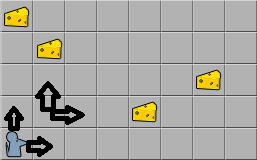
\includegraphics[width=0.5\textwidth]{hw1_a}
\end{center}

Being a mouse and all, Moses wants to gather as much cheese as possible until he reaches the north-east room of the apartment.
\begin{enumerate}
  \item Formulate the problem as a finite horizon decision problem: Define the state space, the action space and the cumulative cost function.
  \item What is the horizon of the problem?
  \item How many possible trajectories are there? How does the number of trajectories behaves as a function of $N$ when $M = 2$? How does it behave as a function of $N$  when $M = N$?
  \item Aharon, Moses's long lost war-buddy woke up confused next to Moses and decided to join him in his quest (needless to say, both mice suffer the same rare head injury).
      \begin{enumerate}
        \item Explain what will happen if both mice ignore each other's existence and act 'optimal' with respect to the original problem.
        \item Assume both mice decided to coordinate their efforts and split the loot. How many states and actions are there now?
        \item Now their entire rarely-head-injured division has joined the journey. Assume there's a total of $K$ mice, how many states and actions are there now?
      \end{enumerate}
\end{enumerate}
\end{exercise}

\begin{exercise}[\textbf{MinMax dynamic programming}]
In this problem we consider an adversarial version of finite horizon dynamic programming, which is suitable for solving 2-player games. 

In this setting, at time $k \in \left\{ {0,1,2, \ldots ,N - 1} \right\}$ the system is at state ${s_k} \in {S_k}$, the agent chooses an action ${a_k} \in {A_k}\left( {{s_k}} \right)$ according to the agent policy $\pi _k^a({s_k})$, and subsequently the opponent chooses an action ${b_k}$ from the set of allowable opponent actions ${B_k}\left( {{s_k},{a_k}} \right)$, according to the opponent policy $\pi _k^b({s_k},{a_k})$.

The system then transitions to a new state according to:
$${s_{k + 1}} = {f_k}({s_k},{a_k},{b_k}),\quad k = 0,1,2, \ldots ,N - 1.$$
The instantaneous reward is denoted by $r\left( {{s_k},{a_k},{b_k}} \right)$, and, for an N-stage path ${h_N} = ({s_0},{a_0},{b_0} \ldots ,{s_{N - 1}},{a_{N - 1}},{b_{N - 1}},{s_N})$ the cumulative reward is
$${R_N}({h_N}) = \sum\limits_{k = 0}^{N - 1} {{r_k}({s_k},{a_k},{b_k}) + {r_N}({s_N})} .$$
Given ${s_0}$, the agent's goal is to find a policy $\pi _a^*$ that maximizes the worst-case cumulative reward:
$$\pi _a^* \in \argmax_{\pi_a} \left\{ {\min_{\pi_b}} \left\{{R_N}({h_N})\right\}\right\}.$$
\begin{enumerate}
  \item Formulate a dynamic programming algorithm for this problem. Explain what the value function represents in this case.
  \item What is the computational complexity of your algorithm?
  \item Could this approach be used to solve the game of tic-tac-toe? Explain what are the states, actions and rewards for this game.
  \item Could this approach be used to solve the game of chess? Explain.
\end{enumerate}
\end{exercise}

\begin{exercise}[\textbf{SSSP}]This exercise concerns the SSSP problem.

\begin{enumerate}
  \item Give an example of a graph that does not contain negative cycles, but for which Dijkstra's algorithm fails. Prove that your graph indeed does not contain any negative cycles.
  \item Consider the following road distances table (Excel file available on the course web-page). Each number in the table represents a road between the two cities of the mentioned distance.
\begin{table}[]
\centering
\resizebox{\textwidth}{!}{%
\begin{tabular}{lllllllllll}
 & Eilat & Ashdod & Beer Sheva & Haifa & Jerusalem & Nazereth & Netanya & Petah Tikva & Rehovot & Tel Aviv \\
Eilat & 0 & 328 & 246 & - & 323 & - & 381 & - & 327 & - \\
Ashdod & 328 & 0 & 82 & - & - & - & - & 47 & 24 & 42 \\
Beer Sheva & 246 & 82 & 0 & - & 89 & - & - & 106 & 82 & 103 \\
Haifa & - & - & - & 0 & 145 & 40 & 64 & 91 &  & 95 \\
Jerusalem & 323 & - & 89 & 145 & 0 & 142 & - & 60 & 59 & 62 \\
Nazereth & - & - & - & 40 & 142 & 0 & 75 & - & - & - \\
Netanya & 381 & - & - & 64 & - & 75 & 0 & 30 & 54 & 33 \\
Petah Tikva & - & 47 & 106 & 91 & 60 & - & 30 & 0 & 29 & 10 \\
Rehovot & 327 & 24 & 82 & - & 59 & - & 54 & 29 & 0 & 21 \\
Tel Aviv & - & 42 & 103 & 95 & 62 & - & 33 & 10 & 21 & 0
\end{tabular}
}
\caption{City-distances}
\end{table}
  \begin{enumerate}
    \item How many nodes and edges are there in the induced graph?
    \item What is the shortest path between Tel Aviv and Haifa? What about Jerusalem and Nazereth?
    \item Program Dijkstra's algorithm and find the shortest path from each city to each other city. What is the time complexity of your solution in terms of the number of nodes and edges in the graph?
    \item Find the shortest route that starts at Jerusalem, visits all other cities and then returns to Jerusalem. What is the time complexity of your solution in terms of the number of nodes and edges in the graph?
  \end{enumerate}
\end{enumerate}
\end{exercise}

\chapter{Markov Decision Processes}

In the previous lectures we considered multi-stage decision problems for \emph{deterministic} systems. In many problems of interest, the system dynamics also involve \emph{randomness}, which leads us to stochastic decision problems. In this chapter we introduce the basic model of Markov Decision Processes, which will be considered is the rest of the course.
%Contents:
%4.1  Markov Chains (Reminder)
%4.2  Controlled Markov Chains
%4.3  Performance Criteria
%4.4 * Sufficiency of Markov policies
%4.4  Finite-horizon Dynamic Programming  (reading assignment)
%
%Note: Corrections (in red) on pages: 2, 3, 7, 13, 16

\section{Markov Chains: A Reminder}

A Markov chain $\{ {X_t},\;t = 0,1,2, \ldots \} $, with ${X_t} \in X$, is a discrete-time stochastic process, over a finite or countable state-space $X$, that satisfies the following Markov property:
	\[{\cal P}({X_{t + 1}} = j|{X_t} = i,{X_{t - 1}}, \ldots {X_0}) = {\cal P}({X_{t + 1}} = j|{X_t} = i).\]
We focus on time-homogeneous Markov chains, where
\[{\cal P}({X_{t + 1}} = j|{X_t} = i) = {\cal P}({X_1} = j|{X_0} = i) \buildrel \Delta \over = {p_{ij}}.\]
The ${p_{ij}}$'s  are the transition probabilities, which satisfy
${p_{ij}} \ge 0,\;\;\;\sum\nolimits_{j \in X} {{p_{ij}} = 1\;\;\forall i} $.
The matrix $P = ({p_{ij}})$ is the transition matrix.

Given the initial distribution ${p_0}$ of ${X_0}$, namely $p({X_0} = i) = {p_0}(i)$, we obtain the finite-dimensional distributions:
\[{\cal P}({X_0} = {i_0}, \ldots ,{X_t} = {i_t}) = {p_0}(i_0){p_{{i_0}{i_1}}} \cdot  \ldots  \cdot {p_{{i_{t - 1}}{i_t}}}.\]

Define $p_{ij}^{(m)} = {\cal P}({X_m} = j|{X_0} = i),$ the m-step transition probabilities.  It is easy to verify that $p_{ij}^{(m)} = {[{P^m}]_{ij}}$  (here ${P^m}$ is the m-th power of the matrix $P$).

\paragraph{State classification:}
\begin{itemize}
\item State $j$ is accessible from $i$  ($i \to j$) if $p_{ij}^{(m)} > 0$ for some $m \ge 1$.
\item $i$ and $j$ are communicating states (or communicate) if $i \to j$ and $j \to i$.
\item A communicating class (or just class) is a maximal collection of states that communicate.
\item The Markov chain is irreducible if all states belong to a single class (i.e., all states communicate with each other).
\item State $i$ is periodic with period $d \ge 2$ if  $p_{ii}^{(m)} = 0$ for $m \ne \ell d$ and  $p_{ii}^{(m)} > 0$ for $m = \ell d$, $\ell \in \{ 1,2, \ldots \}$. Periodicity is a class property: all states in the same class have the same period.
\end{itemize}

\paragraph{Recurrence:}
\begin{itemize}
\item State $i$ is recurrent if ${\cal P}({X_t} = i{ \textrm{ for some }}t \ge 1|{X_0} = i) = 1$. Otherwise, $i$ is transient.
\item State $i$ is recurrent if and only if $\sum\nolimits_{m = 1}^\infty  {p_{ii}^{(m)}}  = \infty $.
\item Recurrence is a class property.
\item If $i$ and $j$ are in the same recurrent class, then $j$ is (eventually) reached from $i$ with probability 1:  ${\cal P}({X_t} = j{\textrm{ for some t}} \ge 1|{X_0} = i) = 1$.
\item Let ${T_i}$ be the return time to state $i$  (number of stages required for $({X_t})$ to return to $i$). If $i$ is a recurrent state, then ${T_i} < \infty $ w.p. 1.
\item State $i$ is positive recurrent if  $E({T_i}) < \infty $, and null recurrent if $E({T_i}) = \infty $.
If the state space is finite, all recurrent states are positive recurrent.
\end{itemize}

\paragraph{Invariant Distribution:} The probability vector $\pi  = ({\pi _i})$ is an invariant distribution or stationary distribution for the Markov chain if $\pi P = \pi ,$ namely
\[{\pi _j} = \sum\nolimits_i^{} {{\pi _i}} {p_{ij}}\quad \forall j.\]
Clearly, if ${X_t} \sim \pi $ then ${X_{t + 1}} \sim \pi $. If ${X_0} \sim \pi $, then the Markov chain $({X_t})$ is a stationary stochastic process.

\begin{theorem}[\textbf{Recurrence of finite Markov chains}] Let $({X_t})$ be an irreducible,  a-periodic Markov chain over a finite state space $X$.  Then the following properties hold:
\begin{enumerate}
\item All states are \textbf{positive recurrent}
\item There exists a \textbf{unique stationary distribution} ${\pi ^*}$
\item \textbf{Convergence} to the stationary distribution: ${\lim _{t \to \infty }}p_{ij}^{(t)} = {\pi _j}\quad (\forall j)$
\item \textbf{Ergodicity}: For any finite $f$: ${\lim _{t \to \infty }}\frac{1}{t}\sum\nolimits_{s = 0}^{t - 1} {f({X_s}) = \sum\nolimits_i {\pi_i f(i) \buildrel \Delta \over = } } \,\pi  \cdot f.$
\end{enumerate}
\end{theorem}

For countable Markov chains, there are other possibilities.

\begin{theorem}[\textbf{Countable Markov chains}]
Let $({X_t})$ be an irreducible and a-periodic Markov chain over a countable state space $X$.  Then:
\begin{enumerate}
\item Either (i) all states are positive recurrent, or (ii) all states are null recurrent, or (iii) all states are transient.
\item If (i) holds, then properties (2)-(4) of the previous Theorem hold as well.
\item Conversely, if there exists a stationary distribution $\pi $ then properties (1)-(4) are satisfied.
\end{enumerate}
\end{theorem}

\paragraph{Reversible Markov chains:} Suppose there exists a probability vector $\pi  = ({\pi _i})$ so that
                                                \begin{equation}\label{eq:DB}
                                                {\pi _i}{p_{ij}} = {\pi _j}{p_{ji}},\quad \quad \forall i,j \in X.
                                                \end{equation}
It is then easy to verify by direct summation that $\pi $ is an invariant distribution for the Markov chain defined by $({p_{ij}})$.
The equations \eqref{eq:DB} are called the \emph{detailed balance equations}. A Markov chain that satisfies these equations is called reversible.

\begin{example}[\textbf{Discrete-time queue}] Consider a discrete-time queue, with queue length $X_t\in \mathbb{N}_0=\{0,1,2,\dots\}$. At time instant $t$, ${A_t}$ new jobs arrive, and then up to ${S_t}$ jobs can be served, so that
\[{X_{t + 1}} = {({X_t} + {A_t} - {S_t})^ + }.\]
Suppose that $({S_t})$ is a sequence of i.i.d. RVs, and similarly $({A_t})$ is a sequence of i.i.d. RVs, with $({S_t})$, $({A_t})$ and ${X_0}$ mutually independent. It may then be seen that
$({X_t},\;t \ge 0)$ is a Markov chain.
Suppose further that each ${S_t}$ is a Bernoulli RV with parameter $q$, namely $P({S_t} = 1) = q$, $P({S_t} = 0) = 1 - q$. Similarly, let ${A_t}$ be a Bernoulli RV with parameter $p$. Then
\[{p_{ij}} = \left\{ {\begin{array}{*{20}{l}}
{p(1 - q)}&:&{j = i + 1}\\
{(1 - p)(1 - q) + pq}&:&{j = i,\;\;i > 0}\\
{(1 - p)q}&:&{j = i - 1,\;\;i > 0}\\
{(1 - p) + pq}&:&{j = i = 0}\\
0&:&{{\rm{otherwise}}}
\end{array}} \right.\]
 Denote $\lambda  = p(1 - q)$, $\mu  = (1 - p)q$, and $\rho  = \lambda /\mu $.   The detailed balance equations for this case are:
\[{\pi _i}\lambda  = {\pi _{i + 1}}\mu ,\quad \quad \forall i \ge 0\]
These equations have a solution with $\sum {_i{\pi _i} = 1}$ if and only if $\rho  < 1$. The solution is ${\pi _i} = {\pi _0}{\rho ^i}$, with ${\pi _0} = 1 - \rho $. This is therefore the stationary distribution of this queue.


\end{example}


\section{Controlled Markov Chains}

A Markov Decision Process consists of two main parts:
\begin{enumerate}
  \item A controlled dynamic system, with stochastic evolution.
  \item A performance objective to be optimized.
\end{enumerate}
In this section we describe the first part, which is modeled as a controlled Markov chain.

Consider a controlled dynamic system, defined over:
\begin{itemize}
  \item A discrete time axis ${\bf{T}} = \{ 0,1, \ldots ,T - 1\} $  (finite horizon), or ${\bf{T}} = \{ 0,1,2, \ldots \} $ (infinite horizon).
To simplify the discussion we refer below to the infinite horizon case, which can always be "truncated" at $T$ if needed.
  \item A finite state space $S$, where ${S_t} \subset S$ is the set of possible states at time $t$ .
  \item A finite action set $A$, where ${A_t}(s) \subset A$ is the set of possible actions at time $t$ and state $s \in {S_t}$.
\end{itemize}

\paragraph{State transition probabilities:}
\begin{itemize}
\item 	Suppose that at time $t$ we are in state ${s_t} = s$, and choose an action ${a_t} = a$. The next state ${s_{t + 1}} = s'$ is then determined randomly according to a probability distribution  ${p_t}( \cdot |s,a)$ on ${S_{t + 1}}$. That is,
\[{\cal P}({s_{t + 1}} = s'|{s_t} = s,{a_t} = a) = {p_t}(s'|s,a),\quad      \quad s' \in {S_{t + 1}}\]
\item 	The probability ${p_t}(s'|s,a)$ is the \emph{transition probability} from state $s$ to state $s'$ for a given action $a$. We naturally require that
            ${p_t}(s'|s,a) \ge 0$, and $\sum\nolimits_{s' \in {S_{t + 1}}}^{} {{p_t}(s'|s,a)}  = 1$ for all $s \in {S_t},a \in {A_t}(s)$.
\item 	Implicit in this definition is the controlled-Markov property:
\[{\cal P}({s_{t + 1}} = s'|{s_t},{a_t}) = {\cal P}({s_{t + 1}} = s'|{s_t},{a_t}, \ldots ,{s_{0,}}{a_0})\]
\item 	The set of probability distributions
                                \[P = \{ {p_t}( \cdot |s,a)\;\;:\;\;s \in {S_t},a \in {A_t}(s),t \in {\bf{T}}\} \]
is called the \emph{transition law} or \emph{transition kernel} of the controlled Markov process.
\end{itemize}

\paragraph{Stationary Models:}
 	The controlled Markov chain is called stationary or time-invariant if the transition probabilities do not depend on the time $t$. That is:
                     \[\forall t,\quad {p_t}(s'|s,a) \equiv p(s'|s,a),\;\;{S_t} \equiv S,\;\;{A_t}(s) \equiv A(s).\]

\paragraph{Graphical Notation:}
The state transition probabilities of a Markov chain are often illustrated via a state transition diagram, such as in Figure \ref{fig:MC}.

\begin{figure}
  % Requires \usepackage{graphicx}
  \begin{centering}
  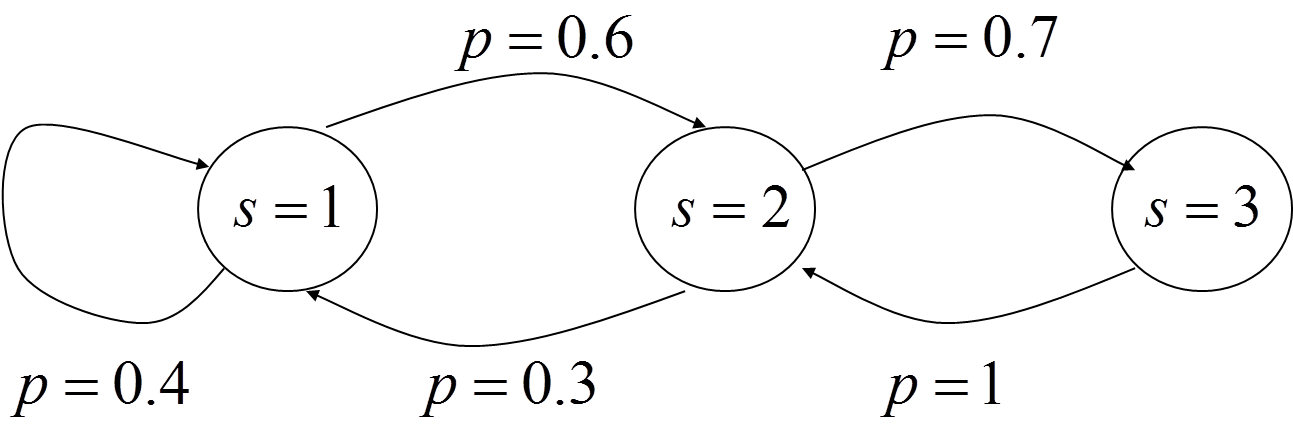
\includegraphics[width=0.7\textwidth]{lecture4_a}\\
  \caption{Markov chain}\label{fig:MC}
  \end{centering}
\end{figure}

A graphical description of a controlled Markov chain is a bit more complicated because of the additional action variable. We obtain the diagram (drawn for state $s = 1$ only, and for a given time $t$) in Figure \ref{fig:MDP}, reflecting the following transition probabilities:
\[\begin{array}{l}
p(s' = 2|s = 1,a = 1) = 1\\
p(s'|s = 1,a = 2) = \left\{ {\begin{array}{*{20}{c}}
{0.3}&:&{s' = 1}\\
{0.2}&:&{s' = 2}\\
{0.5}&:&{s' = 3}
\end{array}} \right.
\end{array}\]

\begin{figure}
  % Requires \usepackage{graphicx}
  \begin{centering}
  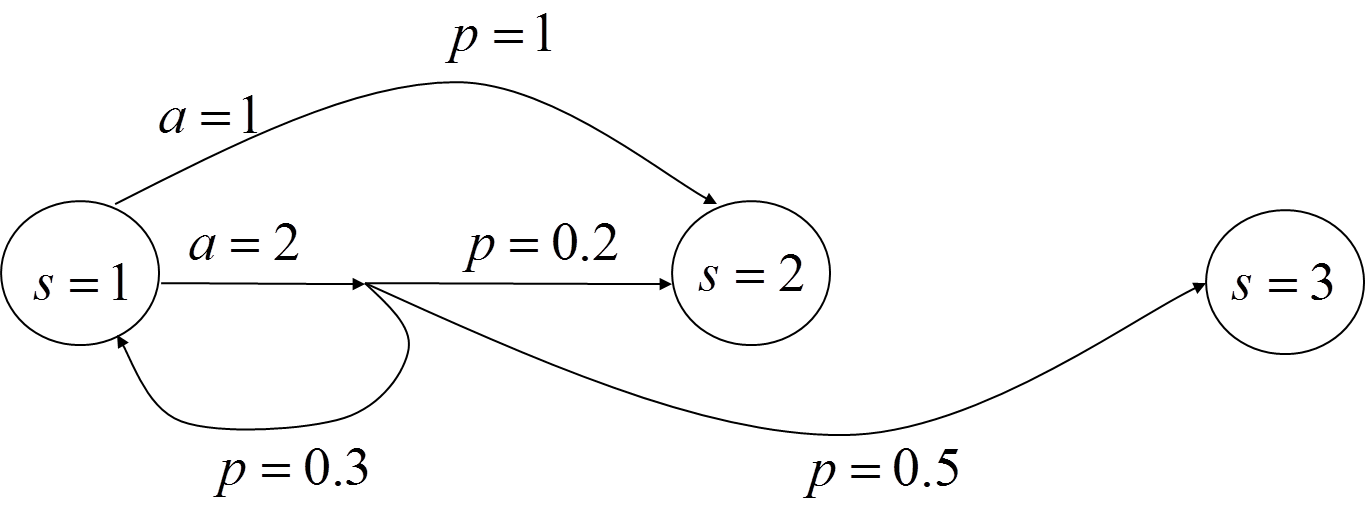
\includegraphics[width=0.7\textwidth]{lecture4_b}\\
  \caption{Controlled Markov chain}\label{fig:MDP}
  \end{centering}
\end{figure}


\paragraph{State-equation notation:}
The stochastic state dynamics can be equivalently defined in terms of a state equation of the form
                                                   \[{s_{t + 1}} = {f_t}({s_t},{a_t},{w_t}),\]
where ${w_t}$ is a random variable.
 	If  ${({w_t})_{t \ge 0}}$ is a sequence of independent RVs, and further each ${w_t}$ is independent of the "past"  $({s_{t - 1}},{a_{t - 1}}, \ldots, {s_0})$, then ${({s_t},{a_t})_{t \ge 0}}$ is a controlled Markov process.
 	For example, the state transition law of the last example can be written in this way, using
                  ${w_t} \in \{ 4,5,6\} $,  with  ${p_w}(4) = 0.3,\;{p_w}(5) = 0.2,\;{p_w}(6) = 0.5$
and, for ${s_t} = 1$:
    \[\begin{array}{l}
 	{f_t}(1,1,{w_t}) = 2\\
 	{f_t}(1,2,{w_t}) = {w_t} - 3
 	\end{array}.\]
The state equation notation is especially useful for problems with continuous state space, but also for some models with discrete states.


\paragraph{Control Policies}
\begin{itemize}
  \item A general or \textbf{history-dependent} control policy $\pi  = {({\pi _t})_{t \in {\bf{T}}}}$ is a mapping from each possible history ${h_t} = ({s_0},{a_0}, \ldots ,{s_{t - 1}},{a_{t - 1}},{s_t})$, $t \in {\bf{T}}$, to an action ${a_t} = {\pi _t}({h_t}) \in {A_t}$.  We denote the set of general policies by ${\Pi _G}$.
  \item A \textbf{Markov} control policy $\pi $ is allowed to depend on the current state and time only: ${a_t} = {\pi _t}({s_t})$.   We denote the set of Markov policies by ${\Pi _M}$.
  \item For stationary models, we may define \textbf{stationary} control policies that depend on the current state alone. A stationary policy is defined by a single mapping $\pi :S \to A$, so that  ${a_t} = \pi ({s_t})$ for all $t \in {\bf{T}}$. We denote the set of stationary policies by ${\Pi _S}$.
  \item Evidently, ${\Pi _G} \supset {\Pi _M} \supset {\Pi _S}$.
\end{itemize}

\paragraph{Randomized Control policies}
\begin{itemize}
  \item The control policies defined above specify deterministically the action to be taken at each stage. In some cases we want to allow for a random choice of action.
  \item A general randomized control policy assigns to each possible history ${h_t}$ a probability distribution ${\pi _t}( \cdot |{h_t})$ over the action set ${A_t}$. That is,  $prob\{ {a_t} = a|{h_t}\}  = {\pi _t}(a|{h_t})$. We denote the set of general randomized policies by ${\Pi _{GR}}$.
  \item Similarly, we can define the set ${\Pi _{MR}}$ of Markov randomized control policies, where ${\pi _t}( \cdot |{h_t})$ is replaced by ${\pi _t}( \cdot |{s_t})$, and the set ${\Pi _{SR}}$ of stationary randomized control policies, where ${\pi _t}( \cdot |{s_t})$ is replaced by  $\pi ( \cdot |{s_t})$.
  \item Note that the set ${\Pi _{GR}}$ includes all other policy sets as special cases.
\end{itemize}

\paragraph{The Induced Stochastic Process}
 	Let  ${p_0} = \{ {p_0}(s),s \in {S_0}\} $ be a probability distribution for the initial state ${s_0}$.
 	A control policy $\pi  \in {\Pi _{GR}}$, together with the transition law $P = \{ {p_t}(s'|s,a)\} $ and the initial state distribution ${p_0} = ({p_0}(s),\;s \in {S_0})$, induce a probability distribution over any finite state-action sequence  ${h_T} = ({s_0},{a_0}, \ldots ,{s_{T - 1}},{a_{T - 1}},{s_T})$, given by
\[P({h_T}) = {p_0}({s_0})\prod\limits_{t = 0}^{T - 1} {p({s_{t + 1}}|{s_t},{a_t}){\pi _t}({a_t}|{h_t})} .\]
To see this, observe the recursive relation:
                      \[\begin{array}{c}
P({h_{t + 1}}) = P({h_t},{a_t},{s_{t + 1}}) = P({s_{t + 1}}|{h_t},{a_t})P({a_t}|{h_t})P({h_t})\\
 = {p_t}({s_{t + 1}}|{s_t},{a_t}){\pi _t}({a_t}|{h_t})P({h_t}).
\end{array}\]
In the last step we used the conditional Markov property of the controlled chain: $P({s_{t + 1}}|{h_t},{a_t}) = {p_t}({s_{t + 1}}|{s_t},{a_t})$, and the definition of the control policy $\pi $.  The required formula follows by recursion.

Therefore, the state-action sequence ${h_\infty } = {({s_k},{a_k})_{k \ge 0}}$ can now be considered a stochastic process. We denote the probability law of this stochastic process by  ${P^{\pi ,{p_0}}}( \cdot )$. The corresponding expectation operator is denoted by ${E^{\pi ,{p_0}}}( \cdot )$.
When the initial state ${s_0}$ is deterministic (i.e., ${p_0}(s)$ is concentrated on a single state $s$), we may simply write ${P^{\pi ,s}}( \cdot )$  or ${P^\pi }( \cdot |{s_0} = s)$.

Under a Markov control policy, the state sequence ${({s_t})_{t \ge 0}}$ becomes a \emph{Markov chain}, with transition probabilities
                            \[P({s_{t + 1}} = s'|{s_t} = s) = \sum\nolimits_{a \in {A_t}} {{p_t}} (s'|s,a){\pi _t}(a|s).\]
\begin{exercise}{Prove this!}\end{exercise}

If the controlled Markov chain is stationary (time-invariant) and the control policy is stationary, then the induced Markov chain is stationary as well.



\begin{remark}
For most non-learning optimization problems, Markov policies suffice to achieve the optimum.
\end{remark}
\begin{remark}
Implicit in these definitions of control policies is the assumption that the current state ${s_t}$ can be fully observed before the action ${a_t}$ is chosen . If this is not the case we need to consider the problem of a Partially Observed MDP (POMDP), which is more involved.
\end{remark}

\section{Performance Criteria}

\subsection{Finite Horizon Problems}
Consider the finite-horizon problem, with a fixed time horizon $T$.
As in the deterministic case, we are given a running reward function ${r_t} = \{ {r_t}(s,a):s \in {S_t},a \in {A_t}\} $ for $0 \le t \le T - 1$, and a terminal reward function ${r_T} = \{ {r_T}(s):s \in {S_T}\} $.  The obtained rewards are then ${R_t} = {r_t}({s_t},{a_t})$ at times $t \le T - 1$, and ${R_T} = {r_T}({s_T})$ at the last stage.
Our general goal is to maximize the cumulative return:
                                             \[\sum\limits_{t = 0}^T {{R_t}}  = \sum\limits_{t = 0}^{T - 1} {{r_t}({s_t},{a_t}) + {r_T}({s_T})} .\]
However, since the system is stochastic, the cumulative return will generally be random, and we need to specify in which sense to maximize it.
A natural first option is to consider the expected value of the return. That is, define:
\[J_T^\pi (s) = {E^\pi }\left(\sum\limits_{t = 0}^T {{R_t}} |{s_0} = s\right) \equiv {E^{\pi ,s}}\left(\sum\limits_{t = 0}^T {{R_t}} \right)\]
 Here $\pi $ is the control policy as defined above, and $s$ denotes the initial state. Hence,  $J_T^\pi (s)$ is the expected cumulative return under the control policy $\pi $.  Our goal is to find an optimal control policy that maximizes $J_T^\pi (s)$.

\paragraph{Remarks:}
\begin{enumerate}
  \item Dependence on the next state:  In some problems, the obtained reward may depend on the next state as well: ${R_t} = {\tilde r_t}({s_t},{a_t},{s_{t + 1}})$.  For control purposes, when we only consider the expected value of the reward, we can reduce this reward function to the usual one by defining:
\[{r_t}(s,a) \buildrel \Delta \over = E({R_t}|{s_t} = s,{a_t} = a) \equiv \sum\nolimits_{s' \in S} {p(s'|s,a){{\tilde r}_t}(} s,a,s')\]
  \item Random rewards:  The reward ${R_t}$ may also be random, namely a random variable whose distribution depends on $({s_t},{a_t})$.  This can also be reduced to our standard model for planning purposes by looking at the expected value of ${R_t}$, namely \[{r_t}(s,a) = E({R_t}|{s_t} = s,{a_t} = a).\]
  \item Risk-sensitive criteria: The expected cumulative return is by far the most common goal for planning. However it is not the only one possible. For example, one may consider the following risk-sensitive  return function:
\[J_{_{T,\lambda }}^\pi (s) = \frac{1}{\lambda }\log {E^{\pi ,s}}(\exp (\lambda \sum\limits_{t = 0}^T {{R_t}} )).\]
For $\lambda  > 0$, the exponent gives higher weight to high rewards, and the opposite for $\lambda  < 0$.
\end{enumerate}

\subsection{Infinite Horizon Problems}
We next consider planning problems that extend to an unlimited time horizon, $t = 0,1,2, \ldots $. Such planning problems arise when the system in question is expected to operate for a long time, or a large number of steps, possibly with no specific "closing" time.
Infinite horizon problems are most often defined for stationary problems. In that case, they enjoy the important advantage that optimal policies can be found among the class of stationary policies.  We will restrict attention here to stationary models.
As before, we have the running reward function $r(s,a)$, which extends to all $t \ge 0$. The reward obtained at stage $t$ is  ${R_t} = r({s_t},{a_t})$.

\paragraph{Discounted return:} The most common performance criterion for infinite horizon problems is the expected discounted return:
\[J_\alpha ^\pi (s) = {E^\pi }\left(\sum\limits_{t = 0}^\infty  {{\alpha ^t}r({s_t},{a_t})} |{s_0} = s\right) \equiv {E^{\pi ,s}}\left(\sum\limits_{t = 0}^\infty  {{\alpha ^t}r({s_t},{a_t})} \right)\]
Here $0 < \alpha  < 1$ is the discount factor. Mathematically, the discount factor ensures convergence of the sum (whenever the reward sequence is bounded). This make the problem "well behaved", and relatively easy to analyze.
\paragraph{Average return:}  Here we are interested in maximizing the long-term average return. The most common definition of the long-term average return is
\[J_{av}^\pi (s) = \mathop {\lim \sup }\limits_{T \to \infty } {E^{\pi ,s}}\left(\frac{1}{T}\sum\limits_{t = 0}^{T - 1} {r({s_t},{a_t})} \right)\]
The theory of average-return planning problems is more involved, and relies to a larger extent on the theory of Markov chains.


\subsection{Stochastic Shortest-Path Problems}
In an important class of planning problems, the time horizon is not set beforehand, but rather the problem continues until a certain event occurs. This event can be defined as reaching some goal state.
Let  ${S_G} \subset S$ define the set of \emph{goal states}. Define
\[\tau  = \inf \{ t \ge 0:{s_t} \in {S_G}\} \]
as the first time in which a goal state is reached. The total expected return for this problem is defined as:
\[J_{ssp}^\pi (s) = {E^{\pi ,s}}\left(\sum\limits_{t = 0}^{\tau  - 1} {r({s_t},{a_t})}  + {r_G}({s_\tau })\right)\]
Here ${r_G}(s),\;s \in {S_G}$ specified the reward at goal states.

This class of problems provides a natural extension of the standard shortest-path problem to stochastic settings.  Some conditions on the system dynamics and reward function must be imposed for the problem to be well posed (e.g., that a goal state may be reached  with probability one).
Such problems are known as stochastic shortest path problems, or also episodic planning problems.

\section{*Sufficiency of Markov Policies}
In all the performance criteria defined above, the criterion is composed of sums of terms of the form $E({r_t}({s_t},{a_t}))$. It follows that if two control policies induce the same marginal probability distributions ${p_t}({s_t},{a_t})$ over the state-action pairs $({s_t},{a_t})$ for all $t \ge 0$, they will have the same performance.

Using this observation, the next claim implies that it is enough to consider the set of (randomized) Markov policies in the above planning problems.

\begin{proposition}\label{prop:sufficient} Let  $\pi  \in {\Pi _{GR}}$ be a general (history-dependent, randomized) control policy.  Let
\[p_t^{\pi ,{s_0}}(s,a) = {P^{\pi ,{s_0}}}({s_t} = s,{a_t} = a),\quad \;\;(s,a) \in {S_t} \times {A_t}\]
Denote the marginal distributions induced by $({s_t},{a_t})$ on the state-action pairs $({s_t},{a_t})$, for all $t \ge 0$.
Then there exists a randomized Markov policy $\tilde \pi $ that induces the same marginal probabilities (for all initial states ${s_0}$).
\end{proposition}
\begin{exercise}[\textbf{Challenge Problem 1}] Prove Proposition \ref{prop:sufficient}.

Note: If you consult a reference or a friend, mention that in your solution.
\end{exercise}


\section{Finite-Horizon Dynamic Programming}

Recall that we consider the expected total reward criterion, which we denote as
\[{J^\pi }({s_0}) = {E^{\pi ,{s_0}}}\left( {\sum\nolimits_{t = 0}^{T - 1} {{r_t}({s_t},{a_t}) + {r_T}({s_T})} } \right)\]
Here $\pi $ is the control policy used, and ${s_0}$ is a given initial state. We wish to maximize ${J^\pi }({s_0})$ over all control policies, and find an optimal policy ${\pi ^*}$ that achieves the maximal reward ${J^*}({s_0})$ for all initial states ${s_0}$.  Thus,
\[{J^*}({s_0}) \buildrel \Delta \over = {J^{\pi *}}({s_0}) = \mathop {\max }\limits_{\pi  \in {\Pi _{GR}}} {J^\pi }({s_0})\]


\subsection{The Principle of Optimality}
The celebrated principle of optimality (stated by Bellman) applies to a large class of multi-stage optimization problems, and is at the heart of DP. As a general principle, it states that:
\begin{center}
\textbf{The tail of an optimal policy is optimal for the "tail" problem.}
\end{center}

This principle is not an actual claim, but rather a guiding principle that can be applied in different ways to each problem.
For example, considering our finite-horizon problem, let ${\pi ^*} = ({\pi _0}, \ldots ,{\pi _{T - 1}})$ denote an optimal Markov policy. Take any state ${s_t} = s'$ which has a positive probability to be reached under ${\pi ^*}$, namely ${P^{\pi^* ,{s_0}}}({s_t} = s') > 0$. Then the tail policy $({\pi _t}, \ldots ,{\pi _{T - 1}})$ is optimal for the "tail" criterion $J_{t:T}^\pi (s') = {E^\pi }\left( {\sum\nolimits_{k = t}^T {{R_k}|{s_t} = s'} } \right)$.


\subsection{Dynamic Programming for Policy Evaluation}\label{sss:pol_eval}
As a "warmup", let us evaluate the reward of a given policy.
Let $\pi  = ({\pi _0}, \ldots ,{\pi _{T - 1}})$ be a given Markov policy. Define the following reward-to-go function, or value function:
\[V_k^\pi (s) = {E^\pi }\left( {\sum\nolimits_{t = k}^T {{R_t}|{s_k} = s} } \right)\]
Observe that $V_0^\pi ({s_0}) = {J^\pi }({s_0})$.

\begin{lemma}[\textbf{Value Iteration}]\label{lem:finite_horizon_VI} $V_k^\pi (s)$ may be computed by the backward recursion:
\[V_k^\pi (s) = {\left\{ {{r_k}(s,a) + \sum\nolimits_{s' \in {S_{k + 1}}} {{p_k}(s'|s,a)} \;V_{k + 1}^\pi (s')} \right\}_{a = {\pi _k}(s)}}\;,\quad s \in {S_k}\]
for $k =  T - 1, \ldots ,0 $,  starting with  $V_T^\pi (s) = {r_T}(s)$.
\end{lemma}
\begin{proof}
Observe that:
\begin{align*}
V_k^\pi (s) &= {E^\pi }\left( {{R_k} + \sum\nolimits_{t = k + 1}^N {{R_t}|} \;{s_k} = s,{a_k} = {\pi _k}(s)} \right)\\
 &= {E^\pi }\left( {{E^\pi }\left( {{R_k} + \sum\nolimits_{t = k + 1}^N {{R_t}} |\;{s_k} = s,{a_k} = {\pi _k}(s),{s_{k + 1}}} \right)|{s_k} = s,{a_k} = {\pi _k}(s)} \right)\\
 &= {E^\pi }\left( {r({s_k},{a_k}) + V_{k + 1}^\pi ({s_{k + 1}})|{s_k} = s,{a_k} = {\pi _k}(s)} \right)\\
 &= {r_k}(s,{\pi _k}(s)) + \sum\nolimits_{s' \in {S_{k + 1}}} {{p_k}(s'|s,{\pi _k}(s))} \;V_{k + 1}^\pi (s')
\end{align*}
\end{proof}
\paragraph{Remarks:}
\begin{itemize}
  \item Note that $\sum\nolimits_{s' \in {S_{k + 1}}} {{p_k}(s'|s,a)} \;V_{k + 1}^\pi (s') = {E^\pi }(V_{k + 1}^\pi ({s_{k + 1}})|{s_k} = s,{a_k} = a)$.
  \item For the more general reward function ${\tilde r_t}(s,a,s')$, the recursion takes the form
                     \[V_k^\pi (s) = {\left\{ {\sum\nolimits_{s' \in {S_{k + 1}}} {{p_k}(s'|s,a)} [{r_k}(s,a,s') + V_{k + 1}^\pi (s')]} \right\}_{a = {\pi _k}(s)}}\]
A similar observation applies to all Dynamic Programming equations below.
\end{itemize}

\subsection{Dynamic Programming for Policy Optimization}

We next define the optimal value function at each time $k \ge 0$ :
\[V_k^{}(s) = \mathop {\max }\limits_{{\pi ^k}} {E^{{\pi ^k}}}\left( {\sum\nolimits_{t = k}^T {{R_t}|{s_k} = s} } \right),\quad \,s \in {S_k}\]
The maximum is taken over "tail" policies ${\pi ^k} = ({\pi _k}, \ldots ,{\pi _{T - 1}})$ that start from time $k$. Note that ${\pi ^k}$ is allowed to be a general policy, i.e., history-dependent and randomized.
Obviously, ${V_0}({s_0}) = {J^*}({s_0})$.

\begin{theorem}[\textbf{Finite-horizon Dynamic Programming}]\label{thm:finite_horizon_DP}
The following holds:
\begin{enumerate}
\item Backward recursion:  Set $V_T^{}(s) = {r_T}(s)$ for $s \in {S_T}$.\\
     For $k = T - 1, \ldots ,0$, $V_k^{}(s)$ may be computed using the following recursion:
\[V_k^{}(s) = \mathop {\max }\limits_{a \in {A_k}} \left\{ {{r_k}(s,a) + \sum\nolimits_{s' \in {S_{k + 1}}} {{p_k}(s'|s,a)\,} V_{k + 1}^{}(s')} \right\},  \quad  s \in {S_k}.\]
\item Optimal policy: Any Markov policy ${\pi ^*}$ that satisfies, for $t = 0, \ldots ,T - 1$,
\[\pi _t^*(s) \in \mathop {\arg \max }\limits_{a \in {A_t}} \left\{ {{r_t}(s,a) + \sum\nolimits_{s' \in {S_{t + 1}}} {{p_t}(s'|s,a)\,} V_{t + 1}^{}(s')} \right\},\quad s \in {S_t},\]
is an optimal control policy. Furthermore, ${\pi ^*}$ maximizes ${J^\pi }({s_0})$ simultaneously
for every initial state ${s_0} \in {S_0}.$
\end{enumerate}
\end{theorem}
Note that Theorem \ref{thm:finite_horizon_DP} specifies an optimal control policy which is a deterministic Markov policy.

\begin{proof}
\textbf{Part (i):}

We use induction to show that the stated backward recursion indeed yields the optimal value function. The idea is simple, but some care is needed with the notation since we consider general policies, and not just Markov policies.
The equality $V_T^{}(s) = {r_T}(s)$ follows directly from the definition of $V_T^{}$.

We proceed by backward induction. Suppose that $V_{k + 1}^{}(s)$ is the optimal value function for time $k + 1$. We need to show that $V_k^{}(s) = {W_k}(s)$, where
                       \[{W_k}(s) \buildrel \Delta \over = {\max _{a \in {A_k}}}\left\{ {{r_k}(s,a) + \sum\nolimits_{s' \in {S_{k + 1}}} {{p_k}(s'|s,a)\,} V_{k + 1}^{}(s')} \right\}.\]
We will first establish that $V_k^{}(s) \ge {W_k}(s)$, and then that $V_k^{}(s) \le {W_k}(s)$.

(a) We first show that $V_k^{}(s) \ge {W_k}(s)$. For that purpose, it is enough to find a policy ${\pi ^k}$ so that $V_k^{{\pi ^k}}(s) = {W_k}(s)$.

Fix $s \in {S_k}$, and define ${\pi ^k}$ as follows: Choose ${a_k} = \bar a$, where
\[\bar a \in \mathop {\arg \max }\limits_{a \in {A_k}} \left\{ {{r_k}(s,a) + \sum\nolimits_{s' \in {S_{k + 1}}} {{p_k}(s'|s,a)} \,V_{k + 1}^{}(s')} \right\},\]
and then, after observing  ${s_{k + 1}} = s'$, proceed with the optimal tail policy ${\pi ^{k + 1}}(s')$ that obtains $V_{k + 1}^{{\pi ^{k + 1}}(s')}(s') = {V_{k + 1}}(s')$. Proceeding similarly to Subsection \ref{sss:pol_eval} above (value iteration for a fixed policy), we obtain:
\begin{align}
V_k^{{\pi ^k}}(s) &= {r_k}(s,\bar a) + \sum\nolimits_{s' \in {S_{k + 1}}} {p(s'|s,\bar a)\,} V_{k + 1}^{{\pi ^{k + 1}}(s')}(s')\\
 &= {r_k}(s,\bar a) + \sum\nolimits_{s' \in {S_{k + 1}}} {p(s'|s,\bar a)} \,V_{k + 1}^{}(s') = {W_k}(s),
\end{align}
as was required.

(b) To establish $V_k^{}(s) \le {W_k}(s)$, it is enough to show that $V_k^{{\pi ^k}}(s) \le {W_k}(s)$ for any (general, randomized) "tail" policy ${\pi ^k}$.

Fix $s \in {S_k}$.
Consider then some tail policy ${\pi ^k} = ({\pi _k}, \ldots {\pi _{T - 1}})$. Note that this means that ${a_t} \sim {\pi _t}(a|{h_{k:t}})$, where ${h_{k:t}} = ({s_k},{a_k},{s_{k + 1}},{a_{k + 1}}, \ldots ,{s_t})$. For each state-action pair $s \in {S_k}$ and $a \in {A_k}$, let  $({\pi ^k}|s,a)$ denote the tail policy ${\pi ^{k + 1}}$ from time $k + 1$ onwards which is obtained from ${\pi ^k}$ given that ${s_k} = s,\;{a_k} = a$. As before, by value iteration for a fixed policy,
\[V_k^{{\pi ^k}}(s) = \sum\nolimits_{a \in {A_k}} {{\pi _k}(a|s)\left\{ {{r_k}(s,a) + \sum\nolimits_{s' \in {S_{k + 1}}} {{p_k}(s'|s,a)} \,V_{k + 1}^{({\pi ^k}|s,a)}(s')} \right\}} .\]
But since $V_{k + 1}^{}$ is optimal,
\begin{align*}
V_k^{{\pi ^k}}(s) &\le \sum\nolimits_{a \in {A_k}} {{\pi _k}(a|s)\left\{ {{r_k}(s,a) + \sum\nolimits_{s' \in {S_{k + 1}}} {{p_k}(s'|s,a)\,} V_{k + 1}^{}(s')} \right\}} \\
 &\le {\max _{a \in {A_k}}}\left\{ {{r_k}(s,a) + \sum\nolimits_{s' \in {S_{k + 1}}} {{p_k}(s'|s,a)\,} V_{k + 1}^{}(s')} \right\} = {W_k}(s),
\end{align*}
which is the required inequality in (b).

\textbf{Part  (ii)} (Outline - \textbf{exercise}):

Let ${\pi ^*}$ be the (Markov) policy defined in part 2 of Theorem \ref{thm:finite_horizon_DP}. Using value iteration for this policy, prove by backward induction that $V_k^{{\pi ^*}} = V_k^{}$.
\end{proof}

\paragraph{To summarize:}
\begin{itemize}
  \item The optimal value function can be computed by backward recursion. This recursive equation is known as the \emph{dynamic programming equation}, \emph{optimality equation}, or \emph{Bellman's Equation}.
  \item Computation of the value function in this way is known as the \emph{finite-horizon value iteration} algorithm.
  \item The value function is computed for all states at each stage.
  \item An optimal policy is easily derived from the optimal value.
  \item The optimization in each stage is performed in the action space.  The total number of minimization operations needed is $T \times |S|$  - each over $|A|$ choices. This replaces "brute force" optimization in policy space, with tremendous computational savings as the number of Markov policies is $|A{|^{T\times |S|}}$.
\end{itemize}

\subsection{The Q function}
Let
\[{Q_k}(s,a) \buildrel \Delta \over = {r_k}(s,a) + \sum\nolimits_{s' \in {S_{k+1}}} {{p_k}(s'|s,a)\,V_{k+1}^{}(s')} .\]
This is known as the optimal state-action value function, or simply as the \emph{Q-function}. ${Q_k}(s,a)$ is the expected return from stage $k$ onward, if we choose ${a_k} = a$  and then proceed optimally.

Theorem \ref{thm:finite_horizon_DP} can now be succinctly expressed as
\[V_k^{}(s) = \mathop {\max }\limits_{a \in {A_k}} {Q_k}(s,a),\]
and
\[\pi _k^*(s) \in \mathop {\arg \max }\limits_{a \in {A_k}} {Q_k}(s,a).\]
The Q function provides the basis for the Q-learning algorithm, which is one of the basic Reinforcement Learning algorithms.




\section{Exercises}
\begin{exercise}[\textbf{Markov chains}]
Let $\left\{ {{X_n}} \right\}$  be a time-homogenous Markov processes in discrete time which takes values in $\left\{ {0,1,..} \right\}$ (an infinite countable set).
\begin{enumerate}
  \item Assume the process satisfies for each $i \in \left\{ {0,1,...} \right\}$:
$${p_{i,0}} = q, \quad {p_{i,i + 1}} = 1 - q, \quad 0 < q < 1.$$
Plot the state transition diagram for $\left\{ {0,1,2,3} \right\}$. If the chain is recurrent, find the stationary distribution, if it is not find the transient states.
  \item Consider the same process as above and assume $P\left( {{X_0} = 0} \right) = 1$. Define ${Y_n} = \left| {\left\{ {\tau :{X_\tau } = 0,\tau  \le n} \right\}} \right|$ as the number of visits to 0 until time $n$. Also define ${Z_n} = {\left( {\begin{array}{*{20}{c}} {{X_n}}&{{Y_n}}\end{array}}\right)^T}$. Is $\left\{ {{Z_n}} \right\}$ a Markov process? Is it recurrent? Is it transient?
  \item Assume the process satisfies for each $i \in \left\{ {1,2,...} \right\}$:
$${p_{0,1}} = 1, \quad {p_{i,i + 1}} = {p_{i,i - 1}} = 0.5.$$
Is the process recurrent? If so, find a stationary distribution if it exists or explain why there is none. If the process is not recurrent, what are the transient states?
\end{enumerate}
\end{exercise}


\chapter{MDPs with Discounted Return}
This lecture covers the basic theory and main solution methods for stationary MDPs over an infinite horizon, with the discounted return criterion. In this case, stationary policies are optimal.

The discounted return problem is the most "well behaved" among all infinite horizon problems (such as average return and stochastic shortest path), and the theory of it is relatively simple, both in the planning and the learning contexts. For that reason, as well as its usefulness, we will consider here the discounted problem and its solution in some detail.

%Contents:
%5.1 Problem Statement
%5.2 Preliminaries: The Fixed-policy Value Function
%5.3 Overview: Main Algorithms
%5.4 Contraction Operators
%5.5 Proof of Bellman's Optimality Equation
%5.6 Value Iteration
%5.7 Policy Iteration
%5.8 Some variants on Value and Policy Iteration
%5.9 Linear Programming Solutions

\section{Problem Statement}\label{sec:inf_horizon_prob}

We consider a stationary (time-invariant) MDP, with a finite state space $S$, finite action set $A$, and transition kernel $P = (P(s'|s,a))$ over the infinite time horizon ${\bf{T}} = \{ 0,1,2, \ldots \} $.

Our goal is to maximize the expected discounted return, which is defined for each control policy $\pi $ and initial state ${s_0} = s$ as follows:
\begin{align*}
J_\gamma ^\pi (s) &= {E^\pi }(\sum\limits_{t = 0}^\infty  {{\gamma ^t}r({s_t},{a_t})} |{s_0} = s)\\
 &\equiv {E^{\pi ,s}}(\sum\limits_{t = 0}^\infty  {{\gamma ^t}r({s_t},{a_t})} )
\end{align*}
Here,
\begin{itemize}
  \item $r : S\times A \to \mathbb R$ is the (running, or instantaneous) reward function.
  \item $\gamma  \in (0,1)$ is the discount factor.
\end{itemize}

We observe that $\gamma  < 1$  ensures convergence of the infinite sum (since the rewards $r({s_t},{a_t})$ are uniformly bounded). With $\gamma  = 1$ we obtain the total return criterion, which is harder to handle due to possible divergence of the sum.

Let $J_\gamma ^*(s)$ denote the maximal value of the discounted return, over all (possibly history dependent and randomized) control policies, i.e.,
\[J_\gamma ^*(s) = \mathop {\sup }\limits_{\pi  \in {\Pi _{GR}}} J_\gamma ^\pi (s).\]


Our goal is to find an optimal control policy ${\pi ^*}$ that attains that maximum (for all initial states), and compute the numeric value of the optimal return $J_\gamma ^*(s)$.
As we shall see, for this problem there always exists an optimal policy which is a  (deterministic) stationary policy.

\textbf{Note:} As usual, the discounted performance criterion can be defined in terms of cost:
\[J_\gamma ^\pi (s) = {E^{\pi ,s}}(\sum\limits_{t = 0}^\infty  {{\gamma ^t}c({s_t},{a_t})} )\]
where $c(s,a)$ is the running cost function. Our goal is then to minimize the discounted cost $J_\gamma ^\pi (s)$.


\section{The Fixed-Policy Value Function}\label{s:FP_VF}

We start the analysis by defining and computing the value function for a fixed stationary policy. This intermediate step is required for later analysis of our optimization problem,  and also serves as a gentle introduction to the value iteration approach.

For a stationary policy $\pi :S \to A$, we define the value function $V_{}^\pi (s),\;s \in S$ simply as the corresponding discounted return:
\[V_{}^\pi (s) \buildrel \Delta \over = {E^{\pi ,s}}\left(\sum\limits_{t = 0}^\infty  {{\gamma ^t}r({s_t},{a_t})} \right)=J_\gamma ^\pi (s),   \quad s \in  S\]

\begin{lemma}\label{lem:FP_Bellman} $V_{}^\pi $ satisfies the following set of $|S|$ linear equations:
\begin{equation}\label{eq:FP_Bellman}
{V^\pi }{\kern 1pt} (s) = r(s,\pi (s)) + \gamma \sum\nolimits_{s' \in S} {p(s'|s,\pi (s)){V^\pi }(s')} \;,\quad \;s \in S.
\end{equation}
\end{lemma}

\begin{proof} We first note that
\begin{align*}
V_{}^\pi (s) &\buildrel \Delta \over = {E^\pi }(\sum\limits_{t = 0}^\infty  {{\gamma ^t}r({s_t},{a_t})} |{s_0} = s)\\
 &= {E^\pi }(\sum\limits_{t = 1}^\infty  {{\gamma ^{t - 1}}r({s_t},{a_t})} |{s_1} = s),
\end{align*}
since both the model and the policy are stationary. Now,
\begin{align*}
V_{}^\pi (s) &= r(s,\pi (s)) + {E^\pi }(\sum\limits_{t = 1}^\infty  {{\gamma ^t}r({s_t},\pi ({s_t}))} |{s_0} = s)\\
&= r(s,\pi (s)) + {E^\pi }\left[\left.{E^\pi }\left(\sum\limits_{t = 1}^\infty  {{\gamma ^t}r({s_t},\pi ({s_t}))} |{s_0} = s, s_1=s'\right)\right|{s_0} = s\right]\\
 &= r(s,\pi (s)) + \sum\limits_{s' \in S}^{} {p(s'|s,\,} \pi (s)){E^\pi }(\sum\limits_{t = 1}^\infty  {{\gamma ^t}r({s_t},\pi ({s_t}))} |{s_1} = s')\\
 &= r(s,\pi (s)) + \gamma \sum\limits_{s' \in S}^{} {p(s'|s,\,} \pi (s)){E^\pi }(\sum\limits_{t = 1}^\infty  {{\gamma ^{t - 1}}r({s_t},{a_t})} |{s_1} = s')\\
 &= r(s,\pi (s)) + \gamma \sum\limits_{s' \in S}^{} {p(s'|s,\,} \pi (s)){V^\pi }(s').
\end{align*}
The first equality is by the smoothing theorem. The second equality follows since ${s_{_0}} = s$ and ${a_t} = \pi ({s_t})$, the third equality follows similarly to the finite-horizon case (Lemma \ref{lem:finite_horizon_VI} in the previous lecture), the fourth is simple algebra, and the last by the observation above.
\end{proof}

We can write the linear equations in \eqref{eq:FP_Bellman} in vector form as follows. Define the column vector ${r^\pi } = {({r^\pi }(s))_{s \in S}}$ with components ${r^\pi }(s) = r(s,\pi (s))$, and the transition matrix ${P^\pi }$ with components ${P^\pi }(s'|s) = p(s'|s,\pi (s))$. Finally, let ${V^\pi }$ denote a column vector with components ${V^\pi }(s)$. Then \eqref{eq:FP_Bellman} is equivalent to the linear equation set
\begin{equation}\label{eq:PF_Bellman_vector}
{V^\pi } = {r^\pi } + \gamma {P^\pi }{V^\pi }
\end{equation}

\begin{lemma}\label{lem:FP_Bellman_sol} The set of linear equations \eqref{eq:FP_Bellman} or \eqref{eq:PF_Bellman_vector}, with ${V^\pi }$ as variables, has a unique solution ${V^\pi }$, which is given by \[{V^\pi } = {(I - \gamma {P^\pi })^{ - 1}}{r^\pi }.\]
\end{lemma}
\begin{proof} We only need to show that the square matrix $I - \gamma {P^\pi }$ is non-singular.  Let $({\lambda _i})$ denote the eigenvalues of the matrix ${P^\pi }$. Since ${P^\pi }$ is a stochastic matrix (row sums are 1), then $|{\lambda _i}| \le 1$. Now, the eignevalues of $I - \gamma {P^\pi }$ are $(1 - \gamma {\lambda _i})$, and satisfy $|1 - \gamma {\lambda _i}| \ge 1 - \gamma  > 0$.                                                                                                            \end{proof}

Combining Lemma \ref{lem:FP_Bellman} and Lemma \ref{eq:PF_Bellman_vector}, we obtain

\begin{proposition}\label{prop:FP_Bellman} The fixed-policy value function ${V^\pi } = [{V^\pi }(s)]$ is the unique solution of equation \eqref{eq:PF_Bellman_vector}, given by \[{V^\pi } = {(I - \gamma {P^\pi })^{ - 1}}{r^\pi }.\]
\end{proposition}

Proposition \ref{prop:FP_Bellman} provides a closed-form formula for computing $V_{}^\pi$. For large systems, computing the inverse ${(I - \gamma {P^\pi })^{ - 1}}$ may be hard.  In that case, the following value iteration algorithm provides an alternative, iterative method for computing $V_{}^\pi$.

\begin{algorithm_}\textbf{Fixed-policy value iteration}
\begin{enumerate}
  \item Let ${V_0} = {({V_0}(s))_{s \in S}}$ be arbitrary.
  \item For $n = 0,1,2, \ldots $, set
\[V_{n + 1}^{}{\kern 1pt} (s) = r(s,\pi (s)) + \gamma \sum\nolimits_{s' \in S} {p(s'|s,\pi (s))V_n^{}{\kern 1pt} (s')} \;,\quad \;s \in S\]
\tab{or, equivalently,}
\[{V_{n + 1}} = {r^\pi } + \gamma {P^\pi }{V_n}.\]
\end{enumerate}
\end{algorithm_}
%Then \[{V_n} \to V_{}^\pi \]component-wise, that is,
%\[{\lim _{n \to \infty }}{V_n}(s) = V_{}^\pi (s),\quad \;s \in S\]

\begin{proposition}[\textbf{Convergence of fixed-policy value iteration}]\label{prop:FP_VI}
We have ${V_n} \to V_{}^\pi$ component-wise, that is,
\[{\lim _{n \to \infty }}{V_n}(s) = V_{}^\pi (s),\quad \;s \in S.\]
\end{proposition}
\begin{proof}
Note first that
\begin{align*}
{V_1}{\kern 1pt} (s) &= r(s,\pi (s)) + \gamma \sum\nolimits_{s' \in S} {p(s'|s,\pi (s))V_0^{}{\kern 1pt} (s')} \;\\
 &= {E^\pi }(r({s_0},{a_0}) + \gamma {V_0}({s_1})|{s_0} = s).
\end{align*}
Continuing similarly, we obtain that
\[{V_n}{\kern 1pt} (s) = {E^\pi }(\sum\limits_{t = 0}^{n - 1} {{\gamma ^t}r({s_t},{a_t})}  + {\gamma ^n}{V_0}({s_n})|{s_0} = s).\]
Note that ${V_n}{\kern 1pt} (s)$ is the $n$-stage discounted return, with terminal reward ${r_n}({s_n}) = {V_0}({s_n})$. Comparing with the definition of $V_{}^\pi $, we can see that
\[{V^\pi }(s) - {V_n}{\kern 1pt} (s) = {E^\pi }(\sum\limits_{t = n}^\infty  {{\gamma ^t}r({s_t},{a_t})}  - {\gamma ^n}{V_0}({s_n})|{s_0} = s).\]
Denoting ${R_{\max }} = {\max _{s,a}}|r(s,a)|$, ${\bar V_0} = {\max _s}|V(s)|$ we obtain
\[|{V^\pi }(s) - {V_n}{\kern 1pt} (s)| \le {\gamma ^n}(\frac{{{R_{\max }}}}{{1 - \gamma }} + {\bar V_0})\]
which converges to 0 since $\gamma  < 1$.                                                                                    �
\end{proof}

\paragraph{Comments:}
\begin{itemize}
  \item The proof provides an explicit bound on $|{V^\pi }(s) - {V_n}{\kern 1pt} (s)|$. It may be seen that the convergence is exponential, with rate $O({\gamma ^n})$.
  \item Using vector notation, it may be seen that
          \[{V_n}{\kern 1pt}  = {r^\pi } + \gamma{P^\pi}{r^\pi } +  \ldots  + \gamma^{n-1}{{(P^\pi)}^{n - 1}}{r^\pi } + \gamma^{n}{{(P^\pi)}^n}{V_0} = \sum\limits_{t = 0}^{n - 1} {\gamma^t{{P^\pi}^t}{r^\pi}}  + {\gamma^n{P^\pi}^n}{V_0}.\]
Similarly,    ${V^\pi } = \sum\limits_{t = 0}^\infty  {\gamma^t{{P^\pi }^t}{r^\pi }}$.
\end{itemize}

\paragraph{In summary:}
\begin{itemize}
  \item Proposition \ref{prop:FP_Bellman} allows to compute $V_{}^\pi $ by solving a set of $|S|$ linear equations.
  \item Proposition \ref{prop:FP_VI} computes $V_{}^\pi $ by an infinite recursion, that converges exponentially fast.
\end{itemize}

\section{Overview: The Main DP Algorithms}

We now return to the optimal planning problem defined in Section \ref{sec:inf_horizon_prob}. Recall that  $J_\gamma ^*(s) = {\sup _{\pi  \in \Pi }}_{_{GR}}J_\gamma ^\pi (s)$ is the optimal discounted return. We further denote
\[{V^*}(s) \buildrel \Delta \over = J_\gamma ^*(s),    \quad s \in S,\]
and refer to ${V^*}$ as the optimal value function. Depending on the context, we consider ${V^*}$ either as a function $V^* : S \to \mathbb R$, or as a column vector ${V^*} = {[V(s)]_{s \in S}}$.

The following optimality equation provides an explicit characterization of the value function, and shows that an optimal stationary policy can easily be computed if the value function is known.

\begin{theorem}[\textbf{Bellman's Optimality Equation}]\label{thm:inf_Bellman} The following statements hold:
\begin{enumerate}
  \item $V_{}^*$ is the unique solution of the following set of (nonlinear) equations:
\begin{equation}\label{eq:Bellman}
V(s) = \mathop {\max }\limits_{a \in A} \left\{ {r(s,a) + \gamma \sum\nolimits_{s' \in S} {p(s'|s,a)V(s')} } \right\},     \quad s \in S.
\end{equation}
  \item Any stationary policy ${\pi ^*}$ that satisfies
\[{\pi ^*}(s) \in \arg {\max _{a \in A}}\left\{ {r(s,a) + \gamma \sum\nolimits_{s' \in S} {p(s'|s,a)V(s')} } \right\},\]
     is an optimal policy (for any initial state ${s_0} \in S$).
\end{enumerate}
\end{theorem}
The optimality equation \eqref{eq:Bellman} is non-linear, and generally requires iterative algorithms for its solution. The main iterative algorithms are \textbf{value iteration} and \textbf{policy iteration}.

\begin{algorithm_}\textbf{Value iteration}\label{alg:VI}
\begin{enumerate}
  \item Let ${V_0} = {({V_0}(s))_{s \in S}}$ be arbitrary.
  \item For $n = 0,1,2, \ldots $, set
\[{V_{n + 1}}(s) = \mathop {\max }\limits_{a \in A} \left\{ {r(s,a) + \gamma \sum\nolimits_{s' \in S} {p(s'|s,a){V_n}(s')} } \right\},    \quad \forall s \in S\]
\end{enumerate}
\end{algorithm_}

\begin{theorem}[\textbf{Convergence of value iteration}]\label{thm:_VI}
We have ${\lim _{n \to \infty }}{V_n} = V_{}^*$ (component-wise). The rate of convergence is exponential, at rate  $O({\gamma ^n})$.
\end{theorem}

The value iteration algorithm iterates over the value functions, with asymptotic convergence. The policy iteration algorithm iterates over stationary policies, with each new policy better than the previous one. This algorithm converges to the optimal policy in a finite number of steps.

\begin{algorithm_}\textbf{Policy iteration}\label{alg:PI}
\begin{enumerate}
\item Initialization: choose some stationary policy ${\pi _0}$.
\item For $k = 0,1, \ldots $:
\begin{enumerate}
\item Policy evaluation: compute ${V^{{\pi _k}}}$.
     \coderemark{For example, use the explicit formula  ${V^{{\pi _k}}} = {(I - \gamma {P^{{\pi _k}}})^{ - 1}}{r^{{\pi _k}}}$.}
\item Policy Improvement: Compute ${\pi _{k + 1}}$, a greedy policy with respect to ${V^{{\pi _k}}}$:
\[{\pi _{k + 1}}(s) \in \arg {\max _{a \in A}}\left\{ {r(s,a) + \gamma \sum\nolimits_{s' \in S} {p(s'|s,a){V^{{\pi _k}}}(s')} } \right\},\quad \forall s \in S.\]
\item Stop if  ${V^{{\pi _{k + 1}}}} = {V^{{\pi _k}}}$ (or if ${V^{{\pi _k}}}$ satisfied the optimality equation), else continue.
\end{enumerate}
\end{enumerate}
\end{algorithm_}

\begin{theorem}[\textbf{Convergence of policy iteration}]\label{thm:_PI}
The following statements hold:
\begin{enumerate}
  \item Each policy ${\pi _{k + 1}}$ is improving over the previous one ${\pi _k}$, in the sense that ${V^{{\pi _{k + 1}}}} \ge {V^{{\pi _k}}}$ (component-wise).
  \item ${V^{{\pi _{k + 1}}}} = {V^{{\pi _k}}}$ if and only if ${\pi _k}$ is an optimal policy.
  \item Consequently, since the number of stationary policies is finite, ${\pi _k}$ converges to the optimal policy after a finite number of steps.
\end{enumerate}
\end{theorem}

An additional solution method for DP planning relies on a Linear Programming formulation of the problem. A Linear Program (LP) is simply an optimization problem with linear objective function and linear constraints. We will provide additional details later in this Lecture.

\section{Contraction Operators}

The basic proof methods of the DP results mentioned above rely on the concept of a \emph{contraction operator}. We provide here the relevant mathematical background, and illustrate the contraction properties of some basic Dynamic Programming operators.

\subsection{The contraction property}
Recall that a norm $|| \cdot ||$ over $\mathbb R^n$  is a real-valued function $\|\cdot\| : \mathbb R^n \to \mathbb R^+$ such that, for any pair of vectors $x,y \in \mathbb R^n$  and scalar $a$,
\begin{enumerate}
  \item $||ax|| = |a| \cdot ||x||$,
  \item $||x + y|| \le ||x|| + ||y||$,
  \item $||x|| = 0$ only if $x = 0$.
\end{enumerate}

Common examples are the p-norm $||x|{|_p} = (\sum\nolimits_{i = 1}^n {{{|{x_i}|}^p}{)^{1/p}}} $ for $p \ge 1$, and in particular the Euclidean norm ($p = 2$). Here we will mostly use the max-norm: \[||x|{|_\infty } = {\max _{1 \le i \le n}}|{x_i}|.\]

Let $T:\mathbb R^d \to \mathbb R^d$  be a vector-valued function over $\mathbb R^d$   ($d \ge 1$). We equip $\mathbb R^d$  with some  norm $|| \cdot ||$, and refer to $T$ as an \emph{operator} over $\mathbb R^d$.  Thus, $T(v) \in \mathbb R^d$ for any $v \in \mathbb R^d$.
We also denote ${T^n}(v) = T({T^{n - 1}}(v))$ for  $n \ge 2$. For example, ${T^2}(v) = T(T(v))$.

\begin{definition} The operator $T$ is called a contraction operator if there exists $\beta  \in (0,1)$ (the contraction coefficient) such that
                            \[||T({v_1}) - T({v_2})|| \le \beta ||{v_1} - {v_2}||,\]
                            for all $v_1,v_2 \in \mathbb R^d$
\end{definition}

\subsection{The Banach Fixed Point Theorem}
The following celebrated result applies to contraction operators. While we quote the result for $\mathbb R^d$, we note that it applies in much greater generality to any Banach space (a complete normed space), or even to any complete metric space, with essentially the same proof.

\begin{theorem}[\textbf{Banach's fixed point theorem}]
Let $T:\mathbb R^d \to \mathbb R^d$  be a contraction operator. Then
\begin{enumerate}
  \item The equation $T(v) = v$ has a unique solution  $V^*\in \mathbb R^d$.
  \item For any $v_0 \in \mathbb R^d$,  ${\lim _{n \to \infty }}{T^n}({v_0}) = {V^*}$.
          In fact,  $||{T^n}({v_0}) - {V^*}|| \le O({\beta ^n})$, where $\beta $ is the contraction coefficient.
\end{enumerate}
\end{theorem}

\begin{proof}
(outline)
\begin{enumerate}
  \item Uniqueness: Let ${V_1}$ and ${V_2}$ be two solutions of $T(v) = v$, then
\[||{V_1} - {V_2}|| = ||T({V_1}) - T({V_2})|| \le \beta ||{V_1} - {V_2}||,\]
which implies that $||{V_1} - {V_2}|| = 0$, hence ${V_1} = {V_2}$.

Existence (outline):  (i) show that ${V_n} \buildrel \Delta \over = {T^n}({V_0})$ (with ${V_0}$ arbitrary) is a Cauchy sequence. (ii) Since any Cauchy sequence in $\mathbb R^d$ converges, this implies that ${V_n}$ converges to some $V^*\in \mathbb R^d$. (iii) Now show that ${V^*}$ satisfies the equation $T(v) = v$.
  \item We have just shown that, for any ${V_0}$, ${V_n} \buildrel \Delta \over = {T^n}({V_0})$ converges to a solution of $T(v) = v$, and that solution was shown before to be unique.  Furthermore, we have
\begin{align*}
||{V_n} - {V^*}||\; &= \;||T({V_{n - 1}}) - T({V^*})||\\
&\le \beta ||{V_{n - 1}} - {V^*}||\;\; \le \;\; \ldots \;\; \le \;{\beta ^n}||{V_0} - {V^*}||\;\;
\end{align*}
\end{enumerate}
\end{proof}


\subsection{The Dynamic Programming Operators}\label{ss:DP_op}
We next define the basic Dynamic Programming operators, and show that they are in fact contraction operators.

For a fixed stationary policy $\pi :S \to A$, define the fixed policy DP operator $T^\pi:\mathbb R^{|S|} \to \mathbb R^{|S|}$  as follows: For any $V=(V(s))\in R^{|S|}$,
\[(T_{}^\pi (V))(s) = r(s,a) + \gamma \sum\nolimits_{s' \in S} {p(s'|s,\pi (s))V(s')} ,\quad s \in S\]
In our column-vector notation, this is equivalent to  $T_{}^\pi (V) = {r^\pi } + \gamma {P^\pi }V$.

Similarly, define the discounted-return \textbf{Dynamic Programming Operator}  $T^*:\mathbb R^{|S|} \to \mathbb R^{|S|}$ as follows: For any $V=(V(s))\in \mathbb R^{|S|}$,
\[(T_{}^*(V))(s) = \mathop {\max }\limits_{a \in A} \left\{ {r(s,a) + \gamma \sum\nolimits_{s' \in S} {p(s'|s,a)V(s')} } \right\},\quad s \in S\]

We note that $T_{}^\pi $ is a linear operator, while $T_{}^*$ is generally non-linear due to the maximum operation.

Let $||V|{|_\infty } \buildrel \Delta \over = {\max _{s \in S}}|V(s)|$ denote the max-norm of $V$.  Recall that $0 < \gamma  < 1$.

\begin{theorem}[\textbf{Contraction property}] The following statements hold:
\begin{enumerate}
  \item $T_{}^\pi $ is a $\gamma$-contraction operator with respect to the max-norm,  namely
                      $||T_{}^\pi ({V_1}) - T_{}^\pi ({V_2})|{|_\infty } \le \gamma ||{V_1} - {V_2}|{|_\infty }$ for all $V_1,V_2\in R^{|S|}$.
  \item Similarly, $T_{}^*$ is an $\gamma$-contraction operator with respect to the max-norm.
\end{enumerate}
\end{theorem}

\begin{proof}
\begin{enumerate}
  \item Fix ${V_1},{V_2}$. For every state $s$,
\begin{align*}
\left| {T_{}^\pi ({V_1})(s) - T_{}^\pi ({V_2})(s)} \right| &= \left| {\gamma \sum\nolimits_{s'} {p(s'|s,\pi (s))[{V_1}(s') - {V_2}(s')]} } \right|\\
 &\le \gamma \sum\nolimits_{s'} {p(s'|s,\pi (s))\left| {{V_1}(s') - {V_2}(s')} \right|} \\
 &\le \gamma \sum\nolimits_{s'} {p(s'|s,\pi (s))} {\left\| {{V_1} - {V_2}} \right\|_\infty } = \gamma {\left\| {{V_1} - {V_2}} \right\|_\infty }\;.
\end{align*}
Since this holds for every $s \in S$ the required inequality follows.
  \item The proof here is more intricate due to the maximum operation. As before, we need to show that  $|T_{}^*({V_1})(s) - T_{}^*({V_2})(s)|\;\, \le \;\,\gamma {\left\| {{V_1} - {V_2}} \right\|_\infty }$. Fixing the state $s$, we consider separately the positive and negative parts of the absolute value:

(a) $T_{}^*({V_1})(s) - T_{}^*({V_2})(s) \le \gamma {\left\| {{V_1} - {V_2}} \right\|_\infty }$:   Let $\bar a$ denote an action that attains the maximum in $T_{}^*({V_1})(s)$, namely $\bar a \in \mathop {\arg \max }\limits_{a \in A} \left\{ {r(s,a) + \gamma \sum\nolimits_{s' \in S} {p(s'|s,a){V_1}(s')} } \right\}$. Then
\[T_{}^*({V_1})(s) = r(s,\bar a) + \gamma \sum\nolimits_{s' \in S} {p(s'|s,\bar a){V_1}(s')} \]
\[T_{}^*({V_2})(s) \ge r(s,\bar a) + \gamma \sum\nolimits_{s' \in S} {p(s'|s,\bar a){V_2}(s')} \]
Since the same action $\bar a$ appears in both expressions, we can now continue to show the inequality (a) similarly to 1.

(b) $T_{}^*({V_2})(s) - T_{}^*({V_1})(s) \le \gamma {\left\| {{V_1} - {V_2}} \right\|_\infty }$:   Follows symmetrically to (a).

The inequalities (a) and (b) together imply that $|T_{}^*({V_1})(s) - T_{}^*({V_2})(s)|\;\, \le \;\,\gamma {\left\| {{V_1} - {V_2}} \right\|_\infty }$. Since this holds for any state $s$, it follows that $||T_{}^*({V_1}) - T_{}^*({V_2})|{|_\infty } \le \gamma {\left\| {{V_1} - {V_2}} \right\|_\infty }$.
\end{enumerate}
\end{proof}


\section{Proof of Bellman's Optimality Equation}
We prove in this section Theorem \ref{thm:inf_Bellman}, which is restated here:
\begin{theorem*}[Bellman's Optimality Equation]
The following statements hold:
\begin{enumerate}
  \item $V_{}^*$ is the unique solution of the following set of (nonlinear) equations:
\begin{equation}\label{eq:Bellman2}
V(s) = \mathop {\max }\limits_{a \in A} \left\{ {r(s,a) + \gamma \sum\nolimits_{s' \in S} {p(s'|s,a)V(s')} } \right\},     \quad s \in S.
\end{equation}
  \item Any stationary policy ${\pi ^*}$ that satisfies
\[{\pi ^*}(s) \in \arg {\max _{a \in A}}\left\{ {r(s,a) + \gamma \sum\nolimits_{s' \in S} {p(s'|s,a)V(s')} } \right\},\]
     is an optimal policy (for any initial state ${s_0} \in S$).
\end{enumerate}
\end{theorem*}
We observe that the Optimality equation in part 1 is equivalent to
$V = {T^*}(V)$
where ${T^*}$ is the optimal DP operator from the previous section, which was shown to be a contraction operator with coefficient $\gamma $.  The proof also uses the value iteration property of Theorem \ref{thm:_VI}, which is proved in the next section.

\begin{proof}[\textbf{Proof of Theorem \ref{thm:inf_Bellman}:}]
We prove each part.
\begin{enumerate}
  \item As $T_{}^*$ is a contraction operator, existence and uniqueness of the solution to $V = T_{}^*(V)$ follows from the Banach fixed point theorem. Let $\hat V$ denote that solution. It also follows by that theorem that ${(T_{}^*)^n}({V_0}) \to \hat V$ for any ${V_0}$. But in Theorem \ref{thm:_VI} we show that ${(T_{}^*)^n}({V_0}) \to V_{}^*$, hence $\hat V = V_{}^*$,  so that $V_{}^*$ is indeed the unique solution of  $V = T_{}^*(V)$.
  \item By definition of  ${\pi ^*}$ we have
\[T_{}^{\pi *}(V_{}^*) = T_{}^*(V_{}^*) = V_{}^*,\]
where the last equality follows from part 1. Thus the optimal value function satisfied the equation $T_{}^{\pi *}V_{}^* = V_{}^*$. But we already know (from Prop. \ref{prop:FP_VI}) that $V_{}^{\pi *}$ is the unique solution of that equation, hence $V_{}^{\pi *} = V_{}^*$. This implies that ${\pi ^*}$ achieves the optimal value (for any initial state), and is therefore an optimal policy as stated.
\end{enumerate}
\end{proof}

\section{Value Iteration}

The value iteration algorithm allows to compute the optimal value function ${V^*}$ iteratively to any required accuracy.
The Value Iteration algorithm (Algorithm \ref{alg:VI}) can be stated as follows:
\begin{enumerate}
  \item Start with any initial value function ${V_0} = ({V_0}(s))$.
  \item Compute recursively, for $n = 0,1,2, \ldots $,
          \[{V_{n + 1}}(s) = \mathop {\max }\limits_{a \in A} \sum\nolimits_{s' \in S} {p(s'|s,a)[r(s,a,s') + \gamma {V_n}(s')]} ,       \quad \forall s \in S.\]
  \item Apply a stopping rule: obtain a required accuracy (see below).
\end{enumerate}
In terms of the DP operator $T_{}^*$, value iteration is simply stated as:
\[{V_{n + 1}} = T_{}^*({V_n}), \quad n \ge 0.\]
Note that the number of operations for each iteration is $O(|A| \cdot |S{|^2})$.
Theorem \ref{thm:_VI} states that ${V_n} \to V_{}^*$, exponentially fast. The proof follows.

\begin{proof}[\textbf{Proof of Theorem \ref{thm:_VI}:}]  Using our previous results on value iteration for the finite-horizon problem, it follows that
\[{V_n}(s) = \mathop {\max }\limits_\pi  {E^{\pi ,s}}(\sum\limits_{t = 0}^{n - 1} {{\gamma ^t}{R_t} + } {\gamma ^n}{V_0}({s_n})).\]
Comparing to the optimal value function
\[{V^*}(s) = \mathop {\max }\limits_\pi  {E^{\pi ,s}}(\sum\limits_{t = 0}^\infty  {{\gamma ^t}{R_t}} ),\]
it may be seen that that
                                \[|{V_n}(s) - V_{}^*(s)| \le {\gamma ^n}(\frac{{{R_{\max }}}}{{1 - \gamma }} + ||{V_0}|{|_\infty }).\]
As $\gamma  < 1$, this implies that ${V_n}$ converges to $V_\gamma ^*$  exponentially fast.                        \end{proof}


\subsection{Error bounds and stopping rules:}
It is important to have an on-line criterion for the accuracy of the n-th step solution ${V_n}$. The exponential bound in the last theorem is usually too crude and can be improved. Since our goal is to find an optimal policy, we need to know how errors in ${V^*}$ affect the sub-optimality of the derived policy. We quote some useful bounds without proof.  More refined error bounds can be found in the texts on Dynamic Programming.

\begin{enumerate}
  \item The distance of ${V_n}$ from the optimal solution is upper bounded as follows:
                                           \[||{V_n} - V_{}^*|{|_\infty } \le {\textstyle{\gamma  \over {1 - \gamma }}}||{V_n} - {V_{n - 1}}|{|_\infty }\]
Note that the right-hand side depends only on the computed values on the last two rounds, and hence is easy to apply. As the bound also decays exponentially (with rate $\gamma $), it allows to compute the value function to within any required accuracy. In particular, to ensure $||{V_n} - V_{}^*|{|_\infty } \le \varepsilon $, we can use the stopping rule  $||{V_n} - {V_{n - 1}}|{|_\infty } \le {\textstyle{{1 - \gamma } \over \gamma }}\varepsilon $.

\item If $||V - V_{}^*|{|_\infty } \le \varepsilon $, then any stationary policy $\pi $ that is greedy with respect to $V$, i.e., satisfies
\[\pi (s) \in \arg {\max _{a \in A}}\left\{ {r(s,a) + \gamma \sum\nolimits_{s' \in S} {p(s'|s,a){V}(s')} } \right\},\]
is $2\varepsilon $-optimal, namely $||V_{}^\pi  - V_{}^*|{|_\infty } \le 2\varepsilon $.
This allows obtain a $2\varepsilon $-optimal policy from an $\varepsilon $-approximation of  $V_{}^*$.
\end{enumerate}

\section{Policy Iteration}

The policy iteration algorithm, introduced by Howard (1960), computes an optimal policy ${\pi ^*}$ in a finite number of steps. This number is typically small (on the same order as $|S|$).

The basic principle behind Policy Iteration is Policy Improvement. Let $\pi$ be a stationary policy, and let $V_{}^\pi $ denote  its value function. A stationary policy $\bar \pi $ is called $\pi$- improving if it is a greedy policy with respect to ${V^\pi }$, namely
\[\bar \pi (s) \in \arg {\max _{a \in A}}\left\{ {r(s,a) + \gamma \sum\nolimits_{s' \in S} {p(s'|s,a){V^\pi }(s')} } \right\}, \quad s \in S.\]

\begin{lemma}[Policy Improvement] We have
${V^{\bar \pi }} \ge {V^\pi }$ (component-wise), and equality holds if and only if  $\pi $ is an optimal policy.
\end{lemma}

\begin{proof} Observe first that
\[{V^\pi } = T_{}^\pi ({V^\pi }) \le T_{}^*({V^\pi }) = T_{}^{\bar \pi }({V^\pi })\]
The first equality follows since ${V^\pi }$ is the value function for the policy $\pi $, the inequality follows because of the maximization in the definition of  $T_{}^*$, and the last equality by definition of the improving policy $\bar \pi $.

It is easily seen that $T_{}^\pi $ is a monotone operator (for any policy $\pi $), namely ${V_1} \le {V_2}$ implies $T_{}^\pi {V_1} \le T_{}^\pi {V_2}$. Applying $T_{}^{\bar \pi }$  repeatedly to both sides of the above inequality ${V^\pi } \le T_{}^{\bar \pi }{V^\pi }$ therefore gives
\[{V^\pi } \le T_{}^{\bar \pi }({V^\pi }) \le {(T_{}^{\bar \pi })^2}({V^\pi }) \le  \cdots  \le \mathop {\lim }\limits_{n \to \infty } {(T_{}^{\bar \pi })^n}({V^\pi }) = {V^{\bar \pi }},\]
where the last equality follows by value iteration. This establishes the first claim.
The equality claim is left as an \textbf{exercise}.
\end{proof}

The policy iteration algorithm performs successive rounds of policy improvement, where each policy ${\pi _{k + 1}}$ improves the previous one ${\pi _k}$. Since the number of stationary policies is bounded, so is the number of strict improvements, and the algorithm must terminate with an optimal policy after a finite number of steps.

In terms of computational complexity, Policy Iteration requires $O(|A|\, \cdot \,|S{|^2}\, + |S{|^3})$ operations per step, with the number of steps being typically small.
 In contrast, Value Iteration requires $O(|A| \cdot |S{|^2})$ per step, but the number of required iterations may be large, especially when the discount factor $\gamma $ is close to 1.


\section{Some Variants on Value Iteration and Policy Iteration}

\subsection{Value Iteration - Gauss Seidel Iteration}
In the standard value iteration: ${V_{n + 1}} = T_{}^*({V_n})$, the vector ${V_n}$ is held fixed while all entries of ${V_{n + 1}}$ are updated.
An alternative is to update each element ${V_n}(s)$ of that vector as to ${V_{n + 1}}(s)$ as soon as the latter is computed, and continue the calculation with the new value.
This procedure is guaranteed to be "as good" as the standard one, in some sense, and often speeds up convergence.


\subsection{Asynchronous Value  Iteration}
Here, in each iteration ${V_n} \Rightarrow {V_{n + 1}}$, only a subset of the entries of  ${V_n}$ (namely, a subset of all states) is updated.
It can be shown that if each state is updated infinitely often, then ${V_n} \to {V^*}$.
Asynchronous update can be used to focus the computational effort on "important'' parts of a large-state space.



\subsection{Modified (a.k.a. Generalized or Optimistic) Policy Iteration}\label{ss:mod_PI}

This scheme combines policy improvement steps with value iteration for policy evaluation. This way the requirement for exact policy evaluation (computing  ${V^{{\pi _k}}} = {(I - \gamma {P^{{\pi _k}}})^{ - 1}}{r^{{\pi _k}}}$) is avoided.

The procedure starts with some initial value vector ${V_0}$, and iterates as follows:
\begin{itemize}
  \item Greedy policy computation:

Compute ${\pi _k} \in \arg {\max _\pi }T_{}^\pi ({V_k})$, a greedy policy with respect to ${V_k}$.
  \item Partial value iteration:

Perform ${m_k}$ steps of value iteration, ${V_{k + 1}} = {(T_{}^{{\pi _k}})^{{m_k}}}({V_k})$.
\end{itemize}

This algorithm guarantees convergence of ${V_k}$ to ${V^*}$.

\section{Linear Programming Solutions}

An alternative approach to value and policy iteration is the linear programming method. Here the optimal control problem is formulated as a linear program (LP), which can be solved efficiently using standard LP solvers. There are two formulations: primal and dual. As this method is less related to learning we will only sketch it briefly.

\subsection{Some Background on Linear Programming}
A Linear Program (LP) is an optimization problem that involves minimizing (or maximizing) a linear objective function subject to linear constraints. A standard form of a LP is
\begin{equation}\label{eq:LP}
 \textrm{minimize } {b^T}x,   \quad \textrm{subject to } Ax \ge c,  x \ge 0.
\end{equation}
where $x = {({x_1},{x_2}, \ldots ,{x_n})^T}$ is a vector of real variables arranged as a column vector.
The set of constraints is linear and defines a \emph{convex polytope} in $\mathbb R^n$, namely a closed and convex set $U$ that is the intersection of a finite number of half-spaces. $U$ has a finite number of vertices, which are points that cannot be generated as a convex combination of other points in  $U$. If  $U$ is bounded, it equals the convex combination of its vertices. It can be seen that an optimal solution (if finite) will be in one of these vertices.

The LP problem has been extensively studied, and many efficient solvers exist. In 1947, Danzig introduced the Simplex algorithm, which essentially moves greedily along neighboring vertices.  In the 1980's effective algorithms (interior point and others) were introduced which had polynomial time guarantees.

\paragraph{Duality:} The \emph{dual} of the LP in \eqref{eq:LP} is defined as the following LP:
\begin{equation}\label{eq:LP_dual}
\textrm{maximize } {c^T}y,   \quad \textrm{subject to } {A^T}y \le b,  y \ge 0.
\end{equation}
The two dual LPs have the same optimal value, and the solution of one can be obtained from that of the other. The common optimal value can be understood by the following computation:

\begin{align*}
\mathop {\min }\limits_{x \ge 0,Ax \ge c} {b^T}x &= \mathop {\min }\limits_{x \ge 0} \mathop {\max }\limits_{y \ge 0} \left\{ {{b^T}x + {y^T}(c - Ax)} \right\}\\
 &= \mathop {\max }\limits_{y \ge 0} \mathop {\min }\limits_{x \ge 0} \left\{ {{c^T}y + {x^T}(b - {A^T}y)} \right\} = \mathop {\max }\limits_{y \ge 0,{A^T}y \le b} {c^T}y.
\end{align*}
where the second equality follows by the min-max theorem.

\paragraph{Note:} For an LP of the form:
\begin{equation*}
 \textrm{minimize } {b^T}x,   \quad \textrm{subject to } Ax \ge c,
\end{equation*}
%minimize \[{b^T}x\],   subject to \[Ax \ge c\],
the dual is
\begin{equation*}
\textrm{maximize } {c^T}y,   \quad \textrm{subject to } {A^T}y = b,  y \ge 0.
\end{equation*}
%maximize \[{c^T}y\],   subject to \[{A^T}y = b\],  \[y \ge 0\]

\subsection{The Primal LP}
Recall that ${V^*}$ satisfies the optimality equations:
\[V(s) = \mathop {\max }\limits_{a \in A} \left\{ {r(s,a) + \gamma \sum\nolimits_{s' \in S} {p(s'|s,a)V(s')} } \right\},     \quad s \in S.\]
\begin{proposition}\label{prop:LP_prop}
${V^*}$ is the smallest function (component-wise) that satisfies the following set of
inequalities:
\begin{equation}\label{eq:LP_prop}
v(s) \ge r(s,a) + \gamma \sum\nolimits_{s' \in S} {p(s'|s,a)v(s')} ,\quad \forall s,a.
\end{equation}
\end{proposition}
\begin{proof}
Suppose $v = (v(s))$ satisfies \eqref{eq:LP_prop}. That is, $v \ge T_{}^\pi (v)$ for every stationary policy. Then by the monotonicity of $T_{}^\pi $,
\[v \ge T_{}^\pi (v)\;\; \Rightarrow \;\;T_{}^\pi (v)\; \ge {(T_{}^\pi )^2}(v)\;\; \Rightarrow \;\; \ldots \; \Rightarrow \;\;{(T_{}^\pi )^k}(v)\; \ge {(T_{}^\pi )^{k + 1}}(v),\]
so that
\[v \ge T_{}^\pi (v) \ge {(T_{}^\pi )^2}(v) \ge  \ldots  \ge \mathop {\lim }\limits_{n \to \infty } {(T_{}^\pi )^n}(v) = {V^\pi }.\]
Now, if we take $\pi$  as the optimal policy we obtain $v \ge {V^*}$ (component-wise).
\end{proof}
It follows from Proposition \ref{prop:LP_prop} that ${V^*}$ is the solution of the following linear program:
\paragraph{Primal LP:	}
\[\mathop {\min }\limits_{(v(s))} \;\;\sum\limits_s {v(s)}, \quad \textrm{ subject to \eqref{eq:LP_prop} } .\]
Note that the number of inequality constraints is ${N_S}\times{N_A}$.

\subsection{The Dual LP}
The dual of our Primal LP turns out to be:

\paragraph{Dual LP:} 	\[\mathop {\max }\limits_{({f_{s,a}})} \quad \;\sum\limits_{s,a} {{f_{s,a}}r(s,a)} \]
   		subject to:	\[{f_{s,a}} \ge 0\quad \forall s,a\]
				\[\sum\limits_{s,a} {{f_{s,a}}}  = {\textstyle{1 \over {1 - \gamma }}}\]
				\[{p_0}(s') + \gamma \sum\limits_{s,a} {p(} s'|s,a){f_{s,a}} = \sum\limits_{a} {{f_{s',a}}\quad \forall s'}  \in S\]
where ${p_0} = ({p_0}(s'))$ is any probability vector (usually taken as a 0/1 vector).

\paragraph{Interpretation:}
\begin{enumerate}
  \item The variables ${f_{s,a}}$ correspond to the "state action frequencies" (for a given policy):
                            \[{f_{s,a}} \sim E(\sum\limits_{t = 0}^\infty  {{\gamma ^t}{I_{\{ {s_t} = s,{a_t} = a\} }})}  = \sum\limits_{t = 0}^\infty  {{\gamma ^t}P({s_t} = s,{a_t} = a)}, \]
and ${p_0}(s') \sim p({s_0} = s')$ is the initial state distribution.
  \item It is easy to see that the discounted return can be written in terms of ${f_{s,a}}$ as $\sum\limits_s {{f_{s,a}}r(s,a)} $, which is to be maximized.
  \item The above constraints easily follow from the definition of ${f_{s,a}}$.
\end{enumerate}
\paragraph{Further comments:}
\begin{itemize}
  \item The optimal policy can by obtained directly from the solution of the dual using:
                                           \[\pi (a|s) = \frac{{{f_{s,a}}}}{{{f_s}}} \equiv \frac{{{f_{s,a}}}}{{\sum\nolimits_a {{f_{s,a}}} }}\]
This policy can be stochastic if the solution to the LP is not unique. However, it will be deterministic even in that case if we choose $f$ as an \emph{extreme} solution of the LP.
  \item The number of constraints in the dual is ${N_S}{N_A} + ({N_S} + 1)$. However, the inequality constraints are simpler than in the primal.
\end{itemize}

\section{Exercises}

\begin{exercise}
You are inside a shady casino with your not so bright friend Jack. You sit at the first table you see and the dealer offers you the following game: he presents you with a Markov Decision Process where you start at ${s_0}$ and can take one of two actions in each state. The transition and rewards for each action are given as follows:
\begin{center}
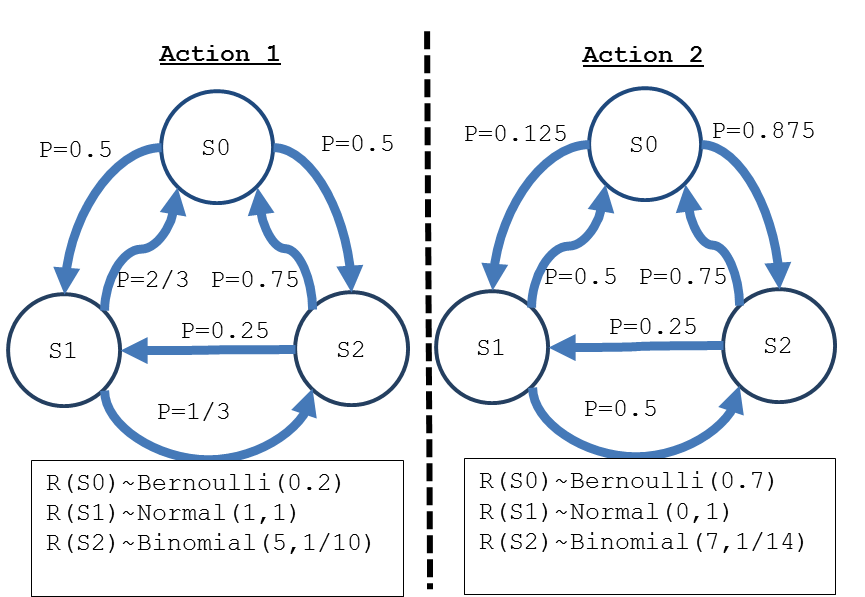
\includegraphics[width=0.8\textwidth]{hw3_a}
\end{center}
\begin{enumerate}
  \item You allow Jack to play a few rounds. Since 21 is his favorite number, Jack starts with the action 2, followed by the action 1 then again action 2 and so on. What is Jack's expected reward after 3 rounds (i.e., 3 actions)?
  \item Jack changes his strategy and starts a new game (at ${s_0}$) choosing the action to be either 1 or 2 with equal probability. What will be Jack's expected reward after 3 rounds now? What is the induced stationary policy over the states?
  \item Write and solve Bellman equations for 3 rounds. What is the optimal policy?
  \item Assuming each round there is a $\beta $ probability of getting thrown out of the casino, write down the infinite horizon cumulative reward. Conclude the connection between the discount factor and the death rate of a process.
  \item Write the Bellman equations for the infinite horizon discounted case in this problem.
\end{enumerate}
\end{exercise}

\begin{exercise}[\textbf{Modeling an Inventory MDP}]
In this question we will model resource allocation problems as MDPs. For each given scenario, write down what are the corresponding states, actions, state-transitions and reward. Also, write down a suitable performance criteria.

\textbf{Remark:} there may be multiple ways to model each scenario. Write down what you think is the most reasonable.

\begin{enumerate}
  \item Consider managing a hot-dog stand. At each hour, starting from 08:00, you decide how many hot-dogs to order from your supplier, each costing $c$, and they arrive instantly. At each hour, the number of hot-dog costumers is a random variable with Poisson distribution with rate $r$, and each customer buys a hot-dog for price $p$. At time 22:00 you close the stand, and throw away the remaining unsold hot-dogs.
  \item Consider scenario (1), but now each supplied hot-dog can only stay fresh for three hours, and then it has to be thrown away.
  \item Consider scenario (1), but now during 12:00-14:00 costumers arrive at double rate.
  \item Consider scenario (1), but now the stand is operated non-stop 24 hours a day. In addition, there is a yearly inflation ratio of 3\%.
  \item Consider scenario (4), but now during 12:00-14:00 costumers arrive at double rate.
\end{enumerate}
\end{exercise}

\begin{exercise}
Prove the following equality (from Section \ref{s:FP_VF} of the lecture notes)
\begin{align*}
V_{}^\pi (s) &\buildrel \Delta \over = {E^\pi }(\sum\limits_{t = 0}^\infty  {{\gamma ^t}r({s_t},{a_t})} |{s_0} = s)\\
 &= {E^\pi }(\sum\limits_{t = 1}^\infty  {{\gamma ^{t - 1}}r({s_t},{a_t})} |{s_1} = s).
\end{align*}
\end{exercise}

\begin{exercise}[\textbf{The $c \mu$ rule}]\label{ex:c_mu}
Assume $N$ jobs are scheduled to run on a single server. At each time step $(t=0,1,2,�)$, the sever may choose one of the remaining unfinished jobs to process. If job $i$ is chosen, then with probability ${\mu _i} > 0$ it will be completed, and removed from the system; otherwise the job stays in the system, and remains in an unfinished state.

Notice that the job service is memoryless - the probability of a job completion is independent of the number of times it has been chosen.
Each job is associated with a waiting cost ${c_i} > 0$ that is paid for each time step that the job is still in the system. The server's goal is minimizing the total cost until all jobs leave the system.
\begin{enumerate}
  \item Describe the problem as a Markov decision process. Write Bellman's equation for this problem.
  \item Show that the optimal policy is choosing at each time step ${i^*} = \argmax_i {c_i}{\mu _i}$ (from the jobs that are still in the system).

  \textbf{Hint: }Compute the value function for the proposed policy and show that it satisfies the Bellman equation.
\end{enumerate}
Remark: the $c\mu $ law is a fundamental result in queuing theory, and applies also to more general scenarios.
\end{exercise}

\begin{exercise}[\textbf{Blackjack}]
Black Jack is a popular casino card game. The object is to obtain a hand with the maximal sum of card values, but without exceeding 21. All face cards count as 10, and the ace counts as 11 (unlike the original game). In our version, each player competes independently against the dealer, and the card deck is infinite (i.e., the probability of drawing a new card from the deck does not depend on the cards in hand).

The game begins with two cards dealt to the player and one to the dealer. If the player starts with 21 it is called a natural (an ace and a 10 card), and he wins (reward = 1).
If the player did not start with 21 he can request additional cards one by one (hits), until he either chooses to stop (sticks) or exceeds 21 (goes bust). If he goes bust, he loses (reward=-1), if he sticks - then it becomes the dealer's turn.
The dealer first draws a second card. Then, the dealer hits or sticks according to a fixed policy: he sticks on any sum of 17 or greater.
If the dealer busts, then the player wins (reward = 1). Otherwise, the outcome--win, lose, or draw--is determined by whose final sum is closer to 21.

We represent a state as $\left( {X,Y} \right)$ where $X$  is the current player sum and $Y$ is the dealer's first card.
\begin{enumerate}
  \item Describe the problem as a Markov decision process. What is the size of the state space?
  \item Use value iteration to solve the MDP. Plot the optimal value function ${V^*}$ as a function of $\left( {X,Y} \right)$.
  \item Use the optimal value function to derive an optimal policy. Plot the optimal policy as follows: for each value of the dealer's card ($Y$), plot the minimal value for which the policy sticks.
\end{enumerate}
Here's an example of the plots you should provide (the values should be different though)
\begin{center}
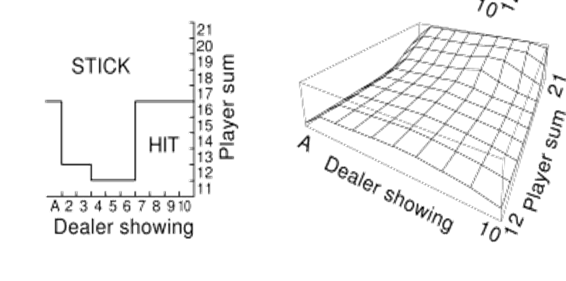
\includegraphics[width=0.7\textwidth]{hw3_b}
\end{center}
\end{exercise}

\begin{exercise}[\textbf{DP operator not contracting in Euclidean norm}]
Recall the fixed-policy DP operator ${T^\pi }$ defined as (see Section \ref{ss:DP_op})
\[\left( {{T^\pi }\left( J \right)} \right)\left( s \right) = r\left( {s,\pi (s)} \right) + \gamma {\sum _{s' \in S}}p\left( {s'|s,\pi (s)} \right)J\left( {s'} \right),\]
where $\gamma  < 1$. We have seen that ${T^\pi }$ is a contraction in the sup-norm. Show that ${T^\pi }$ is not necessarily a contraction in the Euclidean norm.

\textbf{Hint: }one possible approach is to consider the following 2-state MDP, and choose appropriate values for ${p_1},{p_2},\gamma $ to obtain a contradiction to the contraction property.
\begin{center}
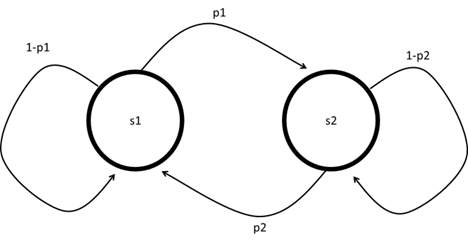
\includegraphics[width=0.6\textwidth]{hw3_c}
\end{center}
\end{exercise}

\begin{exercise}[\textbf{Contraction of ${\left( {{T^*}} \right)^k}$ }]
Recall that the Bellman operator ${T^*}$  defined by
\[\left( {{T^*}\left( J \right)} \right)\left( s \right) = {\max _{a \in A}}\left\{ {r\left( {s,a} \right) + \gamma {\sum _{s' \in S}}p\left( {s'|s,a} \right)J\left( {s'} \right)} \right\}\]
is a $\gamma$-contraction. We will show that ${\left( {{T^*}} \right)^k}$ is a ${\gamma ^k}$-contraction.
\begin{enumerate}
  \item For some $J$  and $\bar J$ let $c = {\max _s}\left| {J\left( s \right) - \bar J\left( s \right)} \right|$. Show that
\begin{equation}\label{eq:ex3a}
{\left( {{T^*}} \right)^k}\left( {J - ce} \right) \le {\left( {{T^*}} \right)^k}\left( {\bar J} \right) \le {\left( {{T^*}} \right)^k}\left( {J + ce} \right),
\end{equation}
where $e$ is a vector of ones.
  \item Now use \eqref{eq:ex3a} to show that  ${\left( {{T^*}} \right)^k}$ is a ${\gamma ^k}$-contraction.
\end{enumerate}
\end{exercise}

\begin{exercise}[\textbf{Second moment and variance of return}]
In the lectures we have defined the value function $V_{}^\pi (s)$ as the expected discounted return when starting from state $s$ and following policy $\pi $,
\[V_{}^\pi (s) = {E^{\pi ,s}}(\sum\limits_{t = 0}^\infty  {{\gamma ^t}r({s_t},{a_t})} ).\]
We have seen that $V_{}^\pi (s)$ satisfies a set of  $|S|$ linear equations (Bellman equation)
\[{V^\pi }{\kern 1pt} (s) = r(s,\pi (s)) + \gamma \sum\nolimits_{s' \in S} {p(s'|s,\pi (s)){V^\pi }(s')} \;,\quad \;s \in S.\]
We now define $M_{}^\pi (s)$ as the second moment of the discounted return when starting from state $s$ and following policy $\pi $,
\[M_{}^\pi (s) = {E^{\pi ,s}}\left( {{{\left( {\sum\limits_{t = 0}^\infty  {{\gamma ^t}r({s_t},{a_t})} } \right)}^2}} \right).\]
\begin{enumerate}
  \item We will show that $M_{}^\pi (s)$ satisfies a 'Bellman like' set of equations. Write an expression for $M_{}^\pi (s)$ that has a linear dependence on $M_{}^\pi $ and  $V_{}^\pi $.

\textbf{Hint:} start by following the derivation of the Bellman equation for $V_{}^\pi .$
  \item How many equations are needed to solve in order to calculate $M_{}^\pi (s)$ for all $s \in S$ ?
  \item We now define $W_{}^\pi (s)$ as the variance of the discounted return when starting from state $s$ and following policy $\pi $,
\[W_{}^\pi (s) = {\rm{Va}}{{\rm{r}}^{\pi ,s}}\left( {\sum\limits_{t = 0}^\infty  {{\gamma ^t}r({s_t},{a_t})} } \right).\]
Explain how $W_{}^\pi (s)$ may be calculated.
\end{enumerate}
\end{exercise}

\begin{exercise}
Consider the modified policy iteration scheme of Section \ref{ss:mod_PI}.
Show that extreme values of ${m_k}$ (which?) reduce this algorithm to the standard Value Iteration or Policy Iteration.
\end{exercise}


% \chapter{Planning in Bandits Problems}
% %\documentclass[11pt]{article}
%\usepackage{geometry}                % See geometry.pdf to learn the layout options. There are lots.
%\geometry{letterpaper}                   % ... or a4paper or a5paper or ...
%%\geometry{landscape}                % Activate for for rotated page geometry
%%\usepackage[parfill]{parskip}    % Activate to begin paragraphs with an empty line rather than an indent
%\usepackage{graphicx}
%\usepackage{amssymb}
%\usepackage{epstopdf}
%\usepackage{amsfonts}
%\usepackage{amsthm}
%\usepackage{amsmath}
%\usepackage{tikz}
%\usepackage{algorithm2e}
%\usepackage{url}
%\usepackage{comment}

%\newcommand{\mdp}{\mathcal{M}}
%\newcommand{\Mdp}{\mathcal{M}}
%\newcommand{\Agent}{\mathcal{G}}
%\newcommand{\env}{\mdp}
%\newcommand{\Env}{\mdp}
%\newcommand{\Actions}{\mathcal{A}}
%\newcommand{\action}{a}
%\newcommand{\actionp}{a^{\prime}}
%\newcommand{\actionpp}{a^{\prime\prime}}
%\newcommand{\States}{\mathcal{S}}
%\newcommand{\state}{s}
%\newcommand{\statep}{\state^{\prime}}
%\newcommand{\statepp}{\state^{\prime\prime}}
%\newcommand{\eststate}{x}

%\newcommand{\obs}{o}
%\newcommand{\Obs}{\mathcal{O}}
%\newcommand{\reward}{r}
%\newcommand{\terminalreward}{r^T}
%\newcommand{\rew}{\reward}
%\newcommand{\Rewards}{\mathcal{R}}
%\newcommand{\history}{h}
%\newcommand{\histories}{\mathcal{H}}
%\newcommand{\Histories}{\mathcal{H}}
%\newcommand{\Trans}{T}
%\newcommand{\Horizon}{t_f}
%\newcommand{\TUtility}{U_T}
%\newcommand{\Utility}{U_{\gamma}}
%\newcommand{\AUtility}{U_A}
%\newcommand{\TValue}{J}
%\newcommand{\TAValue}{K}
%\newcommand{\Value}{V}
%\newcommand{\hatValue}{{\widehat{V}}}
%\newcommand{\AValue}{Q}
%\newcommand{\hatAValue}{{\widehat{Q}}}
%\newcommand{\AvgRValue}{\rho}
%\newcommand{\hatAvgRValue}{{\widehat{\rho}}}
%\newcommand{\RelValue}{W}
%\newcommand{\hatRelValue}{{\widehat{W}}}

%\newcommand{\stateestfunction}{f_{su}}
%\newcommand{\stateobsfunction}{f_{so}}
%\newcommand{\statetransfunction}{f_{ss}}
%\newcommand{\rewfunction}{f_r}
%\newcommand{\field}[1]{\mathbb{#1}}
%\newcommand{\Reals}{\field{R}}
%%\newcommand{\eqref}[1]{(\ref{#1})}
%\newcommand{\policy}{\pi}
%\newcommand{\hatpolicy}{{\widehat{\pi}}}
%\newcommand{\Policies}{\Pi}
%\newcommand{\nspolicy}{\mu}

%\newcommand{\union}{\ensuremath{\bigcup}}
%\newcommand{\comps}{\ensuremath{\mathbb{C}}}
%\newcommand{\reals}{\ensuremath{\mathbb{R}}}
%\newcommand{\Var}{\ensuremath{\mathrm{Var}}}
%\newcommand{\var}{\ensuremath{\mathrm{Var}}}
%\newcommand{\E}{\ensuremath{\mathbb{E}}}
%\renewcommand{\P}{\ensuremath{\mathbb{P}}}
%\newcommand{\R}{\ensuremath{\mathbb{R}}}
%\newcommand{\Z}{\ensuremath{\mathbb{Z}}}

%\newcommand{\mixtime}{\tau}
%\newcommand{\epshorizon}{\tau}

%\def\argmax{\operatornamewithlimits{arg\,max}}
%\def\argmin{\operatornamewithlimits{arg\,min}}

%\newcommand{\bydef}{\stackrel{\bigtriangleup}{=}}
%\newcommand\defeq{\stackrel{\mathrm{def}}{=}}
%\newcommand{\half}{\frac{1}{2}}

%\DeclareGraphicsRule{.tif}{png}{.png}{`convert #1 `dirname #1`/`basename #1 .tif`.png}
%
%\newtheorem{proposition}{Proposition}
%\newtheorem{corollary}{Corollary}
%\newtheorem{assumption}{Assumption}
%\newtheorem{lemma}{Lemma}
%\newtheorem{definition}{Definition}
%\newtheorem{theorem}{Theorem}
%\newtheorem{example}{Example}
%\newtheorem{remark}{Remark}
%
%\title{Planning in Bandits Problems}
%\author{Shie Mannor}
%%\date{}                                           % Activate to display a given date or no date
%
%\begin{document}
%\maketitle
%

We now turn to a planning setup where no learning is involved and the model parameters are fully known. In this setting there are again $K$ arms, but now each arm represents a dynamical system. Pulling or activating an arm leads to a change in the system used, while all other arms remain ``frozen." The problem is which arm to choose and when?

The term multi-armed bandits is confusingly used for both the problem where learning is needed to figure out the expected reward and for the problem we study in this chapter. We will call the planning problem the ``planning bandit problem."

\section{Model and Objectives}

%The model - arms, rewards, etc.
We begin by introducing the definition of a \emph{semi-Markov} decision process.
\begin{definition}[\textbf{Semi-Markov decision process}]
A semi-Markov decision process is a tuple $(S,R,T,P)$ where:
\begin{enumerate}
\item $S$ is the state space.
\item $R$ is the reward random variable. It is assumed that the statistics of the reward depend only on the current state.
\item $T$ is the duration random variable. It is assumed that the statistics of the duration depend only on the current state.
\item $P$ is the transition probability. It assumed that the next state depends only on the current state.
\end{enumerate}
Semi-Markov processes, behave similarly to Markov processes only that the duration of every period varies.
\end{definition}

We now describe our model.
There are $K$ bandit processes, each of them is a semi-Markov decision process, with a state space $S_i$.
We let $S_{All} = S_1 \times S_2 \times \ldots  S_K$ denote the overall state space.
If a bandit $i$ is at state $s\in S_i$ and is selected, then a random reward of $R(s)$ is given after a random length of $T(s)$. After $T(s)$ time units, the play is done and bandit $i$ transitions to a state $Y(s)$ which is a random variable.
At this point, the decision maker is free to switch to any other bandit or stay with $i$.

We assume that all the statistics of all the bandits are known. The statistical properties do not change with time and are independent of history, state of other bandits, etc.

A policy is a mapping from all possible states of the bandits to the arms. That is $\pi: S_{all} \to [1:K]$ which at time zero and any subsequent decision time prescribes which bandit to choose as a function of the current states of the $K$ bandits. Note that to describe a policy in general we need an exponential memory.

Given a policy, the time $t_i$ at which the $i$th play starts, and the reward $R_i$ received during the $i$th period, we are interested in maximizing the discounted reward. For some $\beta>0$ we try to maximize:
$$
\E \left[ \sum_{i=1}^\infty R_i e^{-\beta t_i} \right]
$$
for every initial state. We ignore some technical details and assume that $R_i$ and $T_i$ are well behaved ($R_i$ can be assumed to have finite expectation and $T_i$ bounded from below.)

Given the exponential dependence of the state space size $S_{all}$ in $K$, there does not seem to be much hope for the problem to be tractable. We will show that, surprisingly, there exists an optimal policy that decomposes to the different bandits in a certain way.
A policy is optimal if it maximizes the average discounted reward from every state.



\section{Index Policies}

We say that a policy is an {\em priority policy } if there exists an ordering of $S = S_1 \cup S_2 \cdots S_K$ such that at each decision point the bandit whose state is ordered the highest is chosen.

The basic notion of priority policies implies that instead of finding an optimal policy (a mapping from an exponential state space selection of bandits), it is enough to find an ordering. It is not clear why such policies should exist? And if they do, how to compute them?

\paragraph{Equivalent problem:} Before we proceed to prove the existence of such policies, we first demonstrate how the current problem at hand can be transformed to another problem with a modified reward function.

Since we only care about the expected reward rather than the entire the probability distribution of $R(s)$ and $T(s)$, we will be able to convert it to a different problem. We assume that the policy is fixed. Let $s_i$ be the state of the bandit at is played at the $i$th decision. We let $\mathcal{F}_i$ denote all the random realizations of the first $i-1$ choices. In particular, $t_i$ and $s_i$ are determined by the outcomes and the first $i-1$ plays. Conditioned on $\mathcal{F}_i$ the expected discounted reward resulting from the $i$th play is:
$$
e^{-\beta t_i} \E\left[ R(s_i) | s_i \right].
$$
We now consider an alternative reward: when a bandit at state $s$ is played, the rewards are received throughout the duration of that play at a constant rate $r(s)$ where
$$
r(s) = \frac{\E [R(s)]}{\E \left[ \int_0^{T(s)} e^{-\beta t} d t \right]}.
$$
Under the new reward structure, the expected reward resulting from the $i$th play, conditioned on $\mathcal{F}_i$ is given by:
$$
\E \left[ \int_{t_i}^{t_i + T(s_i)} e^{-\beta t}r(s_i)  d  t \Big| \mathcal{F}_i \right] = e^{-\beta t_i} r(s_i)
\E \left[ \int_{0}^{T(s_i)} e^{-\beta t}  d  t \Big| s_i \right] = e^{-\beta t_i} \E[R(s_i)|s_i],
$$
where the last equality is due to the definition of $r(s)$. We conclude that under either reward structure, the infinite-horizon expected reward of any policy is the same.

Under the assumption that all state spaces for the bandits are finite, it turns out that there exists a prioirty policy that is optimal. Note that this does not mean the reverse: not every optimal policy is necessarily a priority policy.

\begin{theorem}\label{th:2.1inTsitsiklis}
If every $S_i$ is finite there exists a priority policy that is optimal.
\end{theorem}
\proof
The proof proceeds by induction on the size of $S=S_1 \cup S_2 \cdots S_K$. Let us denote the size of $S$ by $N$.
For $N=1$ there is a single bandit and the results holds trivially.
Suppose the result holds for {\em all} bandit problems of size $N=L$ for some $L$. We consider a multi-armed problem whose size is $L+1$. We will show that we can derive a prioirty policy for the new problem as well, completing the induction.

Let us pick some $s^*\in S$ such that $r(s^*) = \max_{s \in S} r(s)$. Let $i^*$ be such that $s^* \in S_{i^*}$. The following lemma shows that state $s^*$ can be chosen as the best state.
\begin{lemma}\label{le:Lemma2.1inTsitsiklis}
There exists an optimal policy such that whenever bandit $i^*$ is at state $s^*$, then bandit $i^*$ is played.
\end{lemma}
\proof
The proof is based on an interchange argument. Consider an optimal policy $\pi$ and suppose that at time 0 bandit $i^*$ is at state $s^*$. If policy $\pi$ chooses to play $i^*$, there is nothing to prove. Suppose that $\pi$ prefers to play another bandit. Let $\tau$ be the first time in which $i^*$ is played ($\tau$ is a random variable which may equal $\infty$ if $i^*$ is never played).
We define a new policy, call it $\pi'$, which plays $i^*$ once and then mimics $\pi$. However, when $\pi$ chooses $i^*$ for the first time, policy $\pi'$ skips this play. Let $\overline{r}(t)$ be the reward rate, as a function of time, of policy $\pi$. We have from the definition of $s^*$ that $\overline{r}(t) \le r(s^*)$ for all $t$.
The expected discounted reward, $J(\pi)$ under policy $\pi$ is given by:
$$
J(\pi) = \E \left[ \int_0^\tau \overline{r}(t) e^{-\beta t}  d  t +
e^{-\beta \tau}\int_0^{T(s^*)} r(s^*) e^{-\beta t}  d  t +
\int_{\tau+T(s^*)}^\infty \overline{r}(t) e^{-\beta t}  d  t \right].
$$
Similarly, the expected discounted return under $\pi'$, can be written as:
$$
J(\pi') = \E \left[
\int_0^{T(s^*)} r(s^*) e^{-\beta t}  d  t +
e^{-\beta T(s^*)} \int_0^\tau \overline{r}(t) e^{-\beta t}  d  t +
\int_{\tau+T(s^*)}^\infty \overline{r}(t) e^{-\beta t}  d  t \right].
$$
Subtracting the two we obtain that $J(\pi') \ge J(\pi)$ if:
$$
\E \left[(1- e^{-\beta \tau}) \int_0^{T(s^*)} r(s^*) e^{-\beta t}  d  t \right]\ge
\E \left[(1- e^{-\beta T(s^*)}) \int_0^\tau \overline{r}(t) e^{-\beta t}  d  t \right].
$$
A straightforward calculation shows that if $\overline{r}(t) = r(s^*)$ (for all $t$) the two sides of the above equations would be equal. Since $\overline{r}(t) \le  r(s^*)$ we obtain that the above equation holds and therefore $J(\pi') \ge J(\pi)$.
Since $\pi$ is assumed optimal, so is $\pi'$. But since it is optimal to give priority to $s^*$ at time 0, it much be optimal to give priority to $s^*$ at every decision time by the same argument.
\qed

We now return to the proof of the theorem. We know from Lemma \ref{le:Lemma2.1inTsitsiklis} that there exists an optimal policy in the set of policies that give priority to $s^*$ (i.e., policies that always select $i^*$ when bandit $i^*$ is in state $s^*$. Let's denote this set of policies by $\Pi(s^*)$. We now want to find the optimal policy in $\Pi(s^*)$.

If $s^*$ is the only state in bandit $i^*$, then the policy that always picks $i^*$ is optimal and it is certainly a prioirty policy.
So we can assume that $S_{i^*}$ is not a singleton. Suppose that there exists a state $s\ne s^*$ in bandit $i^*$ and that
this bandit is played. If this play leads to a transition to $s^*$, bandit $i^*$ will be played (at least) until a transition to a state other than $s^*$ occurs since we restrict attention to policies in $\Pi(s^*)$. We view this continuous play of $i^*$ and a transition to a new state as a single (longer) activation of $i^*$. More precisely, we define an equivalent new bandit problem where all the bandits except for $i^*$ remain exactly the same. For $i^*$ we eliminate state $s^*$, and rather whenever a state $s\ne s^*$ is the state of bandit $i^*$ the random duration $\hat{T}(s)$ is now the total time that elapses in the original model until transitioning to a state different than $s^*$.
Recall that $\overline{r}(t)$ is defined as the reward rate at time $t$, i.e., $\overline{r}(t)=r(s(t))$ where $s(t)$ is the state at time $t$.
By the discussion before the theorem, the reward of every policy remains the same if the discounted reward
$\int_0^{\hat{T}(s)} e^{-\beta t} \overline{r}(t)dt$
received during this new action (representing a composite move) is replaced by a constant reward rate of
\begin{equation}\label{eq:2.3inTsitsiklis}
\hat{r}(s) = \frac{\E [\int_0^{\hat{T}(s)} e^{-\beta t } \overline{r}(t) dt]}{\E [\int_0^{\hat{T}(s)} e^{-\beta t }  dt]}
\end{equation}
that is received throughout the duration of play. We therefore obtained a new bandit problem by removing state $s^*$ from bandit $i^*$ and modifying the rewards and transition durations. We call this procedure ``reducing bandit $i^*$ by removing $s^*$".

We can now use the induction. For the new bandit problem we have that the cardinality is $L$ and therefore a prioirty policy exists, denote it by $\hat{\pi}$. It follows that there exists an index policy for the original problem as well. When bandit $i^*$ is in $s^*$, choose $i^*$. In all other cases, follow $\hat{\pi}$.
\qed

Algorithmically, the theorem proposes the following procedure. We let the index of a state $s$ be denoted by $\gamma(s)$. We are looking for an index that will lead to a priority policy: the higher the index of a state, the better the higher its priority.

An Index Algorithms: Repeat until $S$ is empty:
\begin{enumerate}
\item Pick a state $s^*$ such that $r(s^*) = \max_{s\in S} r(s)$ and let $\gamma(s^*) = r(s^*)$. Let $i^*$ be the bandit such that $s^* \in S_{i^*}$.
\item If $S_{i^*}$ is a singleton, remove bandit $i^*$. If it is not, reduce bandit $i^*$ by removing $s^*$.
\end{enumerate}
%\end{document}

Our previous proof and the analysis lead to the following result, which is the celebrated Gittins index theorem:
\begin{theorem}
Let the index of each state be determined according to the index algorithm. Then any priority policy in which the state with higher index have higher priority is optimal.
\end{theorem}
\proof
The proof of Theorem \ref{th:2.1inTsitsiklis} shows that any priority policy that orders the states in the same order as they are picked by the index algorithm is optimal. It only remains to show that $s$ can be picked before $s'$ by the index algorithm if and only if $\gamma(s)\ge \gamma(s')$. In light of the recursive nature of the algorithm, it is enough to show that if $s^*$ is the first one picked by the index algorithm and $q^*$ is the second then $\gamma(s^*)\ge \gamma(q^*)$. Let $i^*$ be such that $s^*\in S_{i^*}$. If $q^*\in S_{i^*}$ then from Equation (\ref{eq:2.3inTsitsiklis}) we have
$$
\gamma(q^*) = \hat{r}(q^*) \le \max_{s\in S} = r(s^*) = \gamma(s^*).
$$
If $q^*\not \in S_{i^*}$, then $\gamma(q^*) = r(q^*) \le r(s^*) = \gamma(s^*)$. \qed

\medskip

It is important to note that the index algorithm essentially works on each bandit separately. This means that there is a decomposability property that allows the computation to be done for each bandit separately.
%
%\end{document}

% \section{Exercises}

\begin{exercise}[\textbf{Gittins index - bandit reduction}]
Recall that a fundamental ingredient in the index algorithm is the bandit reduction procedure. In this question you will explicitly perform this procedure in a simple case.

We assume that at some point of running the algorithm, the bandit ${i^*}$ corresponds to a 3-state MDP with the following reward rates and transition probabilities:
\[r = \left( {\begin{array}{*{20}{c}}
1\\
2\\
3
\end{array}} \right),\quad P = \left( {\begin{array}{*{20}{c}}
{1/4}&{1/2}&{1/4}\\
{1/3}&{1/3}&{1/3}\\
{1/6}&{1/3}&{1/2}
\end{array}} \right),\]
and the durations of all states in ${i^*}$ are deterministic and equal to 1, i.e., $T(s) = 1.$

Assume that ${s^*} = 3,$ and reduce bandit  ${i^*}$ by removing ${s^*}$.
\begin{enumerate}
  \item What are the resulting transitions in the reduced bandit?
  \item What are the distributions of the durations $\hat T(s)$ in the reduced bandit?
  \item What are the reward rates $\hat r(s)$ in the reduced bandit?
\end{enumerate}
\end{exercise}


% \chapter{Learning in Simple Bandits Problems}
% %\documentclass[11pt]{article}
%\usepackage{geometry}                % See geometry.pdf to learn the layout options. There are lots.
%\geometry{letterpaper}                   % ... or a4paper or a5paper or ...
%%\geometry{landscape}                % Activate for for rotated page geometry
%%\usepackage[parfill]{parskip}    % Activate to begin paragraphs with an empty line rather than an indent
%\usepackage{graphicx}
%\usepackage{amssymb}
%\usepackage{epstopdf}
%\usepackage{amsfonts}
%\usepackage{amsthm}
%\usepackage{amsmath}
%\usepackage{tikz}
%\usepackage{algorithm2e}
%\usepackage{url}
%\usepackage{comment}
%
%\newcommand{\mdp}{\mathcal{M}}
%\newcommand{\Mdp}{\mathcal{M}}
%\newcommand{\Agent}{\mathcal{G}}
%\newcommand{\env}{\mdp}
%\newcommand{\Env}{\mdp}
%\newcommand{\Actions}{\mathcal{A}}
%\newcommand{\action}{a}
%\newcommand{\actionp}{a^{\prime}}
%\newcommand{\actionpp}{a^{\prime\prime}}
%\newcommand{\States}{\mathcal{S}}
%\newcommand{\state}{s}
%\newcommand{\statep}{\state^{\prime}}
%\newcommand{\statepp}{\state^{\prime\prime}}
%\newcommand{\eststate}{x}

%\newcommand{\obs}{o}
%\newcommand{\Obs}{\mathcal{O}}
%\newcommand{\reward}{r}
%\newcommand{\terminalreward}{r^T}
%\newcommand{\rew}{\reward}
%\newcommand{\Rewards}{\mathcal{R}}
%\newcommand{\history}{h}
%\newcommand{\histories}{\mathcal{H}}
%\newcommand{\Histories}{\mathcal{H}}
%\newcommand{\Trans}{T}
%\newcommand{\Horizon}{t_f}
%\newcommand{\TUtility}{U_T}
%\newcommand{\Utility}{U_{\gamma}}
%\newcommand{\AUtility}{U_A}
%\newcommand{\TValue}{J}
%\newcommand{\TAValue}{K}
%\newcommand{\Value}{V}
%\newcommand{\hatValue}{{\widehat{V}}}
%\newcommand{\AValue}{Q}
%\newcommand{\hatAValue}{{\widehat{Q}}}
%\newcommand{\AvgRValue}{\rho}
%\newcommand{\hatAvgRValue}{{\widehat{\rho}}}
%\newcommand{\RelValue}{W}
%\newcommand{\hatRelValue}{{\widehat{W}}}

%\newcommand{\stateestfunction}{f_{su}}
%\newcommand{\stateobsfunction}{f_{so}}
%\newcommand{\statetransfunction}{f_{ss}}
%\newcommand{\rewfunction}{f_r}
%\newcommand{\field}[1]{\mathbb{#1}}
%\newcommand{\Reals}{\field{R}}
%%\newcommand{\eqref}[1]{(\ref{#1})}
%\newcommand{\policy}{\pi}
%\newcommand{\hatpolicy}{{\widehat{\pi}}}
%\newcommand{\Policies}{\Pi}
%\newcommand{\nspolicy}{\mu}
%
%\newcommand{\union}{\ensuremath{\bigcup}}
%\newcommand{\comps}{\ensuremath{\mathbb{C}}}
%\newcommand{\reals}{\ensuremath{\mathbb{R}}}
%\newcommand{\Var}{\ensuremath{\mathrm{Var}}}
%\newcommand{\var}{\ensuremath{\mathrm{Var}}}
%\newcommand{\E}{\ensuremath{\mathbb{E}}}
%\renewcommand{\P}{\ensuremath{\mathbb{P}}}
%\newcommand{\R}{\ensuremath{\mathbb{R}}}
%\newcommand{\Z}{\ensuremath{\mathbb{Z}}}

%\newcommand{\mixtime}{\tau}
%\newcommand{\epshorizon}{\tau}
%
%\def\argmax{\operatornamewithlimits{arg\,max}}
%\def\argmin{\operatornamewithlimits{arg\,min}}

%\newcommand{\bydef}{\stackrel{\bigtriangleup}{=}}
%\newcommand\defeq{\stackrel{\mathrm{def}}{=}}
%\newcommand{\half}{\frac{1}{2}}

%\DeclareGraphicsRule{.tif}{png}{.png}{`convert #1 `dirname #1`/`basename #1 .tif`.png}
%
%\newtheorem{proposition}{Proposition}
%\newtheorem{corollary}{Corollary}
%\newtheorem{assumption}{Assumption}
%\newtheorem{lemma}{Lemma}
%\newtheorem{definition}{Definition}
%\newtheorem{theorem}{Theorem}
%\newtheorem{example}{Example}
%\newtheorem{remark}{Remark}
%
%\title{Learning in Simple Bandits Problems}
%\author{Shie Mannor}
%%\date{}                                           % Activate to display a given date or no date
%
%\begin{document}
%\maketitle
%
%
%

In the classical $k$-armed bandit (KAB) problem there are $k$ alternative arms, each with a stochastic reward whose probability distribution is initially unknown. A decision maker can try these arms in some order, which may depend on the rewards that have been observed so far. A common objective in this context is to find a policy for choosing the next arm to be tried, under which the sum of the expected rewards comes as close as possible to the ideal reward, i.e., the expected reward that would be obtained if we were to try the ``best'' arm at all times.
There are many variants of the $k$-armed bandit problem that are distinguished by the objective of the decision maker, the process governing the reward of each arm, and the information available to the decision maker at the end of every trial.

$K$-armed bandit problems are a family of sequential decision problems that are among the most studied problems in statistics, control, decision theory, and machine learning. In spite of the simplicity of KAB problems, they encompass many of the basic problems of sequential decision making in uncertain environments such as the tradeoff between exploration and exploitation.
There are many variants of the KAB problem including Bayesian, Markovian, adversarial, and exploratory variants. KAB formulations arise naturally in multiple fields and disciplines including communication networks, clinical trials, search theory, scheduling, supply chain automation, finance, control, information technology, etc.
The term ``multi-armed bandit" is borrowed from slot machines (the well known one-armed bandit) where a decision maker has to decide if to insert a coin to the gambling machine and pull a lever possibly getting a significant reward, or to quit without spending any money.

In this chapter we focus on the stochastic setup where the reward of each arm is assumed to be generated by an IID process.


\section{Model and Objectives}

%The model - arms, rewards, etc.

The KAB model is  comprised of a set of arms
$A$ with $K=|A|$. When sampling arm $a\in A$ a reward which is a
random variable $R(a)$ is received.
Denote the arms by $a_1, \cdots , a_n$ and $p_i =\E[R(a_i)]$.
%i.e.,
%viewed as coins, so that
%the $i$-th arm has probability $p_i$ for reward of 1 and
%$1-p_i$ for a reward of 0.
For simplicity of notations we enumerate the arms according to
their expected reward $p_1 > p_2>...>p_n$.

In general, the arm with the highest expected reward is called the {\em best
arm}, and denoted by $a^*$, and its expected reward $r^*$ is the
{\em optimal reward}; with our notational convenience above arm $a^* = 1$ and $ r^* = p_1$. An arm whose expected reward is strictly
less than $r^*$, the expected reward of the best arm, is called a
{\em non-best arm}. An arm $a$ is called an {\em
$\epsilon$-optimal arm} if its expected reward is at most
$\epsilon$ from the optimal reward, i.e., $p_a = \E[R(a)] \geq r^*
-\epsilon$.

An algorithm for the KAB problem, at each time step
$t$, samples an arm $a_t$ and receives a reward $r_t$ (distributed
according to $R(a_t)$). When making its selection the algorithm
may depend on the history (i.e., the actions and rewards) up to
time $t-1$. The algorithm may also randomize between several options, leading to a random policy.
In stochastic KAB problems there is no advantage to a randomized strategy.

%Objectives

There are two common objectives for the KAB problem that represent two different learning scenarios. Those objectives represent different situations. In the first situation, the decision maker only cares about the detecting the best arm or approximately the best arm. The rewards that are accumulated during the learning period are of no concern to the decision maker and he only wishes to maximize the probability of reporting the best arm at the end of the learning period.
Typically, the decision maker is given a certain number of stages to {\em explore} the arms. That is, the decision maker needs to choose an arm which is either optimal or approximately optimal with high probability in a short time. This setup is that of pure exploration.
The second situation is where the reward that is accumulated during the learning period counts. Usually, the decision maker cares about maximizing the cumulative reward\footnote{We consider reward maximization as opposed to cost minimization, but all we discuss here works for minimizing costs as well.}.
The cumulative reward is a random variable: its values are affected by random values generated by selecting the different arms. We typically look at the expected cumulative reward:
$$
 \E \left[ \sum_{\tau=1}^t r_t \right].
$$
In this setup the decision maker has to typically tradeoff between two contradicting desires:
exploration and exploitation. Exploration means finding the best arm and exploitation means choosing the arm that is
believed to be the best so far. The KAB problem is the simplest learning problems where the problem of balancing exploration and exploitation, known as the exploration-exploitation dilemma is observed.
The total expected reward scale linearly with time. It is often more instructive to consider the {\em regret}.
The regret measures the difference between the best reward and the accumulated reward:
$$
regret_t = t r^* - \sum_{\tau=1}^t r_t.
$$
The regret itself is a random variable since the actual reward is a random variable. We therefore focus on the expected regret:
$$
\E [regret_t] = t r^* - \E \Big[ \sum_{\tau=1}^t r_t \Big].
$$
We note that by linearity of expectation, the expected regret is always non-negative. The actual regret, however, can be negative.

\section{Exploration-Exploitation problem setup}

The KAB problem comes with two main flavors: exploration only and exploration-exploitation. Since the arms are assumed IID, this is a simple problem in terms of dynamics. The challenge is that we do not know if we should look for a better arm than the one we currently think is the best or should stick to the arm that is estimated to be the best do far.

A very simple algorithm is the so-called $\epsilon$-greedy algorithm. According to this algorithm, we throw an unbiased coin at every time instance whose probability of getting ``heads" is $\epsilon$.
If the coin falls on ``heads," we choose an arm at random. If it falls on ``tails," we choose the arm whose estimate is the highest so far. The exploration rate, $\epsilon$, may depend on the number of iteration. While the $\epsilon$-greedy algorithm is very simple conceptually, it is not a great algorithm in terms of performance. The main reason is that some of the exploration is useless: we might have enough data to estimate an arm, or at least know with confidence that its value is lower than competing arms, and the additional samples are just not particularly useful.
Instead, there are more elegant algorithms which we will describe below.

%The context (Benner \& Tushman)

%Simple algorithms like epsilon-greedy
%SM: Anything else?

%Successive elimination (throw away ``bad arms")

%\newpage

\section{The Exploratory Multi-armed Bandit Problem}

In this variant the emphasis is on efficient exploration rather than on exploration-exploitation tradeoff. As in the stochastic MAB problem, the decision maker is given access to $n$ arms where each arm is associated with an independent and identically distributed random variable with unknown statistics. The decision maker�s goal is to identify the ``best'' arm. That is the decision maker wishes to find the arm with highest expected reward as quickly as possible.
The exploratory MAB problem is a sequential hypothesis testing problem but with the added complication that the decision maker can choose where to sample next, making it among the simplest active learning problems.


Next we define the desired properties of an algorithm formally.
\begin{definition}
An algorithm is a $(\epsilon,\delta)$-PAC algorithm for the multi
armed bandit with {\em sample complexity} $T$, if it outputs an
$\epsilon$-optimal arm, $a'$, with probability at least
$1-\delta$, when it terminates, and the number of time steps the
algorithm performs until it terminates is bounded by $T$.
\end{definition}


In this section we look for an $(\epsilon,\delta)$-PAC algorithms
for the MAB problem. Such algorithms are required to output with
probability $1 - \delta$ an $\epsilon$-optimal arm. We start with
a naive solution that samples each arm $1/(\epsilon/2)^2
\ln(2n/\delta) $ and picks the arm with the highest empirical
reward. The sample complexity of this naive algorithm is
$O(n/\epsilon^2\log(n/\delta))$. The naive algorithm is described
in Algorithm \ref{alg:naive}. In Section \ref{sub:successive} we
consider an algorithm that eliminates one arm after the other. In
Section \ref{sub:median} we finally describe the Median
Elimination algorithm whose sample complexity is optimal in the
worst case.
%This result in an algorithm whose arm sample complexity is:
%
%\begin{equation}
%\label{eq:basicalg}
%O(\frac{n}{\epsilon^2}\log(\frac{n}{\delta}))\, .
%\end{equation}

\medbreak

\begin{algorithm}[H]
\SetKwInOut{Input}{Input}\SetKwInOut{Output}{Output}
\Input{$\epsilon>0$, $\delta>0$} \Output{An arm}
\ForEach{ {\rm Arm} $a\in A$}{
     Sample it $\ell = \frac{4}{\epsilon^2}\ln(\frac{2n}{\delta})$
     times\;Let $\hat{p}_a$ be the average reward of arm $a$;}
    Output $a'= \arg\max_{a \in A} \{ \hat{p}_a\}$\;
\caption{\label{alg:naive} Naive Algorithm}
%\textbf{Naive}$(\epsilon,\delta)$}
\end{algorithm}

\begin{theorem}
The algorithm {\em Naive}$(\epsilon,\delta)$ is an
$(\epsilon,\delta)$-PAC algorithm with arm sample complexity
$O\left((n/\epsilon^2)\log(n/\delta)\right)$.
\end{theorem}
\proof
The sample complexity is immediate from the
definition of the algorithm (there are $n$ arms and each arm
is pulled $ \frac{4}{\epsilon^2}\ln(\frac{2n}{\delta})$ times). We now prove it is
an $(\epsilon,\delta)$-PAC  algorithm.

Let $a'$ be an arm for which $\E(R(a')) < r^* - \epsilon$. We want to
bound the probability of the event $\hat{p}_{a'}
> \hat{p}_{a^*}$.
\begin{eqnarray*}
P \left(\hat{p}_{a'} > \hat{p}_{a^*}\right) & \le &
P\left(\hat{p}_{a'} >  \E[R(a')] + \epsilon/2 \mbox{ or } \hat{p}_{a^*}
<
r^* -\epsilon/2\right)\\
& \leq & P\left(\hat{p}_{a'} >  \E[R(a')] + \epsilon/2\right) +  P
\left( \hat{p}_{a^*} < r^* -\epsilon/2\right) \\
& \le & 2\exp(- 2(\epsilon/2)^2 \ell)\,,
\end{eqnarray*}
%
where the last inequality uses the Hoeffding inequality. Choosing
$\ell = (2/\epsilon^2)\ln(2n/\delta)$ assures that $P
\left(\hat{p}_{a'} > \hat{p}_{a^*}\right) \le \delta/n$.
Since there are at most $n-1$ such arms $a'$, by the Union Bound, the probability of selecting an arm that is not $\epsilon$-optimal will be at most $\frac{(n-1)\delta}{n} < \delta$, and thus the probability of selecting an $\epsilon$-optimal arm will be at least $1 - \delta$.




%Summing over all possible $a'$ we have that the failure probability is at most $(n-1)(\delta/n) <\delta$.
\qed


\subsection{Successive Elimination}
\label{sub:successive}

The successive elimination algorithm attempts to sample each arm a minimal
number of times and eliminate the arms one after the other.
To motivate the successive elimination algorithm, we first assume that the
expected rewards of the arms are known, but the matching of the
arms to the expected rewards is unknown. Let $\Delta_i = p_{1} -
p_{i} >0$.
Our aim is to sample arm $a_i$ for
$(1/\Delta_i^2) \ln(n/\delta)$ times, and then
eliminate it. This is done in phases. Initially, we sample each
arm $(1/\Delta_n^2)\ln(n/\delta)$ times. Then we
eliminate the arm which has the lowest empirical reward (and never
sample it again). At the $i$-th phase we sample each of the $n-i$
surviving arms
$$O\left(\left(\frac{1}{\Delta_{n-i}^2} -
\frac{1}{\Delta_{n-i+1}^2}\right)\log{(\frac{n}{\delta})}\right)$$
times and
then eliminate the empirically worst arm. The algorithm described as
Algorithm \ref{alg:sucknown} below. In Theorem \ref{th:sucelimknown} we prove
that the algorithm is $(0,\delta)$-PAC and compute its sample complexity.

\medbreak
\begin{algorithm}[H]
\SetKwInOut{Input}{Input}\SetKwInOut{Output}{Output}
\Input{$\delta>0$, bias of arms $p_1,p_2,\ldots, p_n$} \Output{An arm}
Set $S = A$; $t_i =  (8/\Delta_i^2) \ln (2n/\delta)
    $; and $t_{n+1}=0$, for every arm $a$: $\hat{p}_a = 0$,
    $i=0$\;
    \While{$i < n-1$}
    {
    Sample every arm $a \in S$ for $t_{n-i} - t_{n-i+1}$ times\;
    Let $\hat{p}_a$ be the average reward of arm $a$ (in all
    rounds)\;
    Set $S = S \setminus \{a_{\min}\}$, where
    $a_{\min}=\arg\min _{a\in S} \{ \hat{p}_a\}$,
    $i = i + 1$\;
    }
    Output S\;
\caption{Successive Elimination with Known Biases \label{alg:sucknown}}
%$(\delta)$ \label{alg:sucknown}}
\end{algorithm}
\begin{theorem} \label{th:sucelimknown}
Suppose that $\Delta_i>0$ for $i=2,3,\ldots,n$. Then the Successive
Elimination with Known Biases algorithm is an $(0,\delta)$-PAC
algorithm and its arm sample complexity is
\begin{equation} \label{eq:sucelim}
O\left(\log\left(\frac{n}{\delta}\right)\sum_{i=2}^{n}\frac{1}{\Delta_i^2}\right).
\end{equation}
\end{theorem}
\begin{proof}




First we show that the algorithm outputs the best arm with probability $1 - \delta$.
This is done by showing that, in each phase, the probability of eliminating the
best arm is bounded by $\frac{\delta}{n}$. It is clear that the failure probability at phase $i$ is
maximized if all the $i-1$ worst arms have been eliminated in the first $i-1$ phases. Since we eliminate a single arm at each phase of the algorithm, the probability of the best arm being eliminated at phase $i$ is bounded by
$Pr[\hat{p}_1 < \hat{p}_2, \hat{p}_1 < \hat{p}_3, \ldots, \hat{p}_1 < \hat{p}_{n-i}] \leq Pr[\hat{p}_1 < \hat{p}_{n-i}]$.

The probability that $\hat{p}_1 < \hat{p}_{n-i}$, after sampling each arm for $O(\frac{1}{\Delta^2_i}\log\frac{n}{\delta})$ times is bounded by $\frac{\delta}{n}$. Therefore the total probability of failure is bounded by $\delta$.


The sample complexity of the algorithm is as follows.
In the first round we sample $n$ arms $t_n$ times. In the second
round we sample $n-1$ arms $t_{n-1 } - t_n$ times. In the $k$th round ($1\leq k<n$)
we sample $n-k+1$ surviving arms for $t_{n-k} - t_{n-k+1}$ times. The total number of arms samples is therefore
$t_2 + \sum_{i=2}^n t_i$ which is of the form (\ref{eq:sucelim}).\\

\begin{comment}
We now prove that the algorithm is correct with probability at least $1-\delta$.
Consider first a simplified algorithm which is similar to the naive algorithm, suppose that
each arm is pulled $8/(\Delta_{2}^2) \ln(2n/\delta)$ times.
For every $2\le i \le n-1$ we define the event
$$
E_i = \left\{\hat{p_1}^{t_j} \geq \hat{p_i}^{t_j}
|\forall t_j \,{\rm s.t.}\, j \geq i\right\},$$
where  $\hat{p_i}^{t_j}$ is the
empirical value the $i$th arm at time $t_j$. If the events
$E_i$ hold for all $i>1$ the algorithm is successful.
\begin{eqnarray*}
\P[\mbox{not}( E_i)] &\leq& \sum_{j=i}^n \P[\hat{p_n}^{t_j} <
\hat{p_i}^{t_j}]\\
& \leq & \sum_{j=i}^n 2\exp(-2(\Delta_i/2)^2 t_j) \leq \sum_{j=i}^n
2\exp(-2(\Delta_i/2)^2 8/ \Delta_j^2 \ln(2n/ \delta))\\
& \leq & \sum_{j=i}^n 2 \exp (-\ln (4n^2 / \delta^2)) \\
& \leq & (n-i+1) \delta^2/n^2 \leq \frac{\delta}{n}.
\end{eqnarray*}
Using the union bound over all $E_i$'s we obtain that the simplified
algorithm satisfies all $E_i$ with probability at least $1- \delta$.
Consider the original setup. If arm $1$ is eliminated at time $t_j$
for some is implies that some arm $i<j$ has higher empirical value
at time $t_j$. The probability of failure of the here is bounded by
the probability of failure in the simplified setting.
\end{comment}
\end{proof}
%\qed



 Next, we relax the requirement that the expected rewards of the
arms are known in advance, and introduce the Successive Elimination
algorithm that works with any set of biases. The algorithm we
present as Algorithm \ref{alg:sucunknown} finds the best arm (rather
than $\epsilon$-best) with high probability. We later explain in Remark
\ref{rem:epssucc} how
to modify it to be an $(\epsilon,\delta)$-PAC algorithm.\\
\bigskip
\begin{algorithm}[H]
\SetKwInOut{Input}{Input}\SetKwInOut{Output}{Output}
\Input{$\delta>0$} \Output{An arm}
Set $t=1$ and $S = A$\; Set for every arm $a$: $\hat{p}_a^1 = 0$\;
Sample every arm $a \in S$ once and let
    $\hat{p}_a^t$ be the average reward of arm $a$ by time $t$ \textcolor{red}{move into repeat?} \;
    \Repeat{$|S| > 1$\textcolor{red}{=1?}}{
    Let $\hat{p}^t_{max} = \max_{a \in S} \hat{p}_a^t$ and
     $\alpha_t = \sqrt{\ln(c n t^2/ \delta)/t}$, where $c$ is a constant\;
     \ForEach{ {\rm arm $a \in S$ such that } $\hat{p}^t_{max} - \hat{p}^t_a \geq
     2\alpha_t$}{ set $S = S \setminus \{a\}$;}
     $t = t+1$\;
    }
\caption{Successive elimination with unknown biases \label{alg:sucunknown}}
\end{algorithm}

\begin{theorem}
Suppose that $\Delta_i>0$ for $i=2,3,\ldots,n$. Then the Successive
Elimination algorithm (Algorithm \ref{alg:sucunknown}) is a
$(0,\delta)$-PAC algorithm, and with probability at least $1-\delta$
the number of samples is bounded by
$$
O\left(\sum_{i=2}^{n}\frac{\ln(\frac{n}{\delta\Delta_i})}{\Delta_i^2}\right).
$$
\end{theorem}
\begin{proof}
Our main argument is that, at any time $t$ and for any action $a$, the observed probability $\hat{p}_a^t$
is within $\alpha_t$ of the true probability $p_a$.
%Let $\alpha_t=\sqrt{\frac{\ln(c n t^2/ \delta)}{t}}$.
For any time $t$ and action $a\in S_t$ we have that,
\[
\P[ |\hat{p}_a^t -p_a | \geq  \alpha_t ] \leq 2e^{-2\alpha_t^2 t }
\leq \frac{2\delta}{cnt^2}.
\]
By taking the constant $c$ to be greater than 4 and from the union bound we have that
with probability at least $1-\delta/n$ for any
time $t$ and any action $a\in S_t$, $|\hat{p}_a^t -p_a | \leq
\alpha_t$. Therefore, with probability $1-\delta$, the best arm is
never eliminated. Furthermore, since $\alpha_t$ goes to zero as
$t$ increases, eventually every non-best arm is eliminated. This
completes the proof that the algorithm is $(0,\delta)$-PAC.

It remains to compute the arm sample complexity. To eliminate a
non-best arm $a_i$ we need to reach a time $t_i$ such that,
\[
\hat{\Delta}_{t_i} = \hat{p}^{t_i}_{a_1}-\hat{p}^{t_i}_{a_i} \geq
2 \alpha_{t_i}.
\]
The definition of $\alpha_t$ combined with the assumption that
$|\hat{p}_a^t -p_a | \leq  \alpha_t$ yields that
\[
\Delta_i -2\alpha_t = (p_1-\alpha_t) -(p_i +\alpha_t)\geq
\hat{p}_1-\hat{p}_i \geq  2 \alpha_t,
\]
which holds with probability at least $1-\frac{\delta}{n}$ for
\[
t_i=O\left(\frac{\ln (n/\delta\Delta_i)}{\Delta_i^2}\right).
\]
To conclude, with probability of at least $1-\delta$ the number of
arm samples is $2t_2 +\sum_{i=3}^n t_i$, which completes the proof.
\end{proof}

\begin{remark}
{\rm We can improve the dependence on the parameter
$\Delta_i$ if at the $t$-th phase we sample each action in $S_t$
for $2^t$ times rather than once and take $\alpha_t =
\sqrt{\ln(c n \ln(t)/ \delta)/t}$. This will give us a
bound on the number of samples with a dependency of
$$
O\left(\sum_{i=2}^{n}\frac{\log\left(-\frac{n}{\delta}\log(\Delta_i)\right)}{\Delta_i^2}\right).
$$
}
\end{remark}

\begin{remark}
{\rm
\label{rem:epssucc}
One can easily modify the successive
elimination algorithm so that it is $(\epsilon,\delta)$-PAC. Instead
of stopping when only one arm survives the elimination, it is
possible to settle for stopping when either only one arm remains
or when each of the $k$ surviving arms were sampled
$O(\frac{1}{\epsilon ^2} \log(\frac{k}{\delta}))$. In the latter case
the algorithm returns the best arm so far. In this case it is not
hard to show that the algorithm finds an $\epsilon$-optimal arm with
probability at least $1-\delta$ after
$$
O\left(\sum_{i:\Delta_i > \epsilon}
\frac{\log(\frac{n}{\delta\Delta_i})}{\Delta_i^2} +
\frac{N(\Delta, \epsilon)}{\epsilon ^2} \log\left(\frac{N(\Delta, \epsilon)}{\delta}\right)
\right)\,,
$$
where $N(\Delta, \epsilon)= |\{i \;|\; \Delta_i < \epsilon\}|$ is the
number of arms which are $\epsilon $-optimal.
}
\end{remark}


\subsection{Median elimination}
\label{sub:median}

The following algorithm substitutes the term $O(\log (1/\delta))$ for
$O(\log(n/\delta))$ of the naive bound. The idea is
to eliminate the worst half of the arms at each iteration. We do not
expect the best arm to be empirically ``the best,'' we only expect
an $\epsilon$-optimal arm to be above the median.


\begin{algorithm}[H]
\SetKwInOut{Input}{Input}\SetKwInOut{Output}{Output}
\Input{$\epsilon >0, \delta>0$} \Output{An arm}
Set $S_1 = A$, $\epsilon_1 = \epsilon/4$, $\delta_1 = \delta/2$,
$\ell =1$. \Repeat{$|S_\ell| = 1$}{Sample every arm $a \in S_\ell$ for
    $1/(\epsilon_\ell / 2)^2 \log(3 / \delta_\ell)$ times, and
    let $\hat{p}_a^\ell$ denote its empirical value\;
    Find the median of $\hat{p}_a^\ell$, denoted by $m_\ell$\;
    $S_{\ell+1} = S_\ell \setminus \{ a: \hat{p}_a^\ell <
    m_\ell\}$\;
    $\epsilon_{\ell+1} = \frac{3}{4}\epsilon_\ell$;
    $\delta_{\ell+1} = \delta_\ell / 2$; $\ell = \ell + 1$\;
    } \caption{Median Elimination}
%($\epsilon$, $\delta$)}
\end{algorithm}


\begin{theorem}
\label{the-n-coins} The Median Elimination($\epsilon$,$\delta$)
algorithm is an $(\epsilon,\delta)$-PAC algorithm and
%with probability at least $1 - \delta$,
%outputs an $\epsilon$-best arm  and uses
its sample complexity is
$$O\left(\frac{n}{\epsilon^2} \log\left(\frac{1}{\delta}\right)\right).$$
\end{theorem}

%Let $S_\ell$ denote the set of arms in the beginning of the $\ell$-th period.
First we show that in the $\ell$-th phase the expected reward of
the best arm in $S_\ell$ drops by at most $\epsilon_\ell$.

\begin{lemma}
\label{lem-round-n} For the  {\em Median
Elimination}$(\epsilon,\delta)$ algorithm we have that for every phase $\ell$:
\begin{eqnarray*}
\P[\max_{j \in S_\ell}p_j \leq \max_{i \in S_{\ell+1}}p_i +
\epsilon_\ell] \geq 1 -\delta_\ell.
\end{eqnarray*}
\end{lemma}

\begin{proof}
Without loss of generality we look at the first round and assume
that $p_1$ is the reward of the best arm. We bound the failure
probability by looking at the event $E_1 = \{\hat{p}_1 < p_1 -
\epsilon_1 / 2\}$, which is the case that  the empirical estimate
of the best arm is pessimistic.
%on the two complementing events:
%\begin{itemize}
%\item $E_1 = \hat{p_1} < p_1 - \epsilon_1 / 2$ -
%%the empirical estimate of the best arm is pessimistic.
%\item $E_2 = \hat{p_1} \geq p_1 - \epsilon_1 / 2$ -
%the empirical estimate of the best arm is good.
%\end{itemize}
Since we sample sufficiently, we have that $\P[E_1]  \leq \delta_1
/ 3$.
%This implies
%that any event further conditioned on $E_1$ has also probability of no more
%than $\delta_1 / 3$.

In case $E_1$ does not hold, we calculate the probability that an
arm $j$ which is not an $\epsilon_1$-optimal arm is empirically better
than the best arm.
$$
\P\left[\hat{p}_j \geq \hat{p}_1  \;|\;\hat{p}_1 \geq p_1 -\epsilon_1
/2 \right] \leq
\P\left[ \hat{p}_j \geq p_j +  \epsilon_1 / 2  \;|\;
\hat{p}_1 \geq p_1 -\epsilon_1 / 2 \right] \leq \delta_1 / 3
$$
Let $\#\mbox{bad}$ be the number of arms which are not
$\epsilon_1$-optimal but are empirically better than the best arm.
We have that $\E[\#\mbox{bad} \;|\;\hat{p}_1 \geq p_1 -\epsilon_1
/2] \le n \delta_1/3$. Next we apply Markov inequality to obtain,
\begin{eqnarray*}
\P[\#\mbox{bad} \geq n/2 \;|\;\hat{p}_1 \geq p_1 -\epsilon_1 /2]
\leq \frac{ n\delta_1 / 3}{n / 2} = 2\delta_1 / 3.
\end{eqnarray*}
Using the union bound gives us that the probability of failure is
bounded by $\delta_1$. \qed
\end{proof}


Next we prove that arm sample complexity is bounded by
$O((n/\epsilon^2) \log(1/\delta))$.

\begin{lemma}
\label{lem-time-n} The sample complexity of the {\em Median Elimination}$(\epsilon,\delta)$
is $O\left((n/\epsilon^2)\log(1/\delta)\right)$.
\end{lemma}

\begin{proof}
%First we observe that the number of iterations is $\log_2(n)$.
The number of arm samples in the $\ell$-th round is $4 n_\ell\log(3 / \delta_\ell)/\epsilon_\ell^2$. By definition we
have that
\begin{enumerate}
\item $\delta_1 = \delta /2\enspace ; \enspace \delta_\ell =
\delta_{\ell-1} / 2 = \delta / 2^\ell$ \item $n_1 = n \enspace ;
\enspace n_\ell = n_{\ell-1} / 2 = n / 2^{\ell-1}$ \item
$\epsilon_1 = \epsilon / 4 \enspace ; \enspace \epsilon_\ell =
\frac{3}{4}\epsilon_{\ell-1} =
\left(\frac{3}{4}\right)^{\ell-1}\epsilon / 4 $
\end{enumerate}
Therefore we have
\begin{eqnarray*}
\sum_{\ell=1}^{\log_2(n)}\frac{n_\ell\log(3 /
\delta_\ell)}{(\epsilon_\ell / 2)^2} & = &
4\sum_{\ell=1}^{\log_2(n)}\frac{n / 2^{\ell-1}\log(2^\ell 3/
\delta)}{((\frac{3}{4})^{\ell-1}\epsilon / 4)^2}\\
& = & 64 \sum_{\ell=1}^{\log_2(n)}
n(\frac{8}{9})^{\ell-1}(\frac{\log(1 / \delta)}{\epsilon^2} +
\frac{\log(3)}{\epsilon^2} +
\frac{\ell \log(2)}{\epsilon^2})\\
& \leq & 64 \frac{n \log(1/\delta)}{\epsilon^2} \sum_{\ell=1}^\infty
(\frac{8}{9})^{\ell-1}( \ell C' +C) = O(\frac{n\log(1
/\delta)}{\epsilon^2})
\end{eqnarray*} \qed
\end{proof}

Now we can prove Theorem \ref{the-n-coins}.

\begin{proof}
 From Lemma \ref{lem-time-n} we have that the sample complexity is
bounded by $O\left(n\log(1 /\delta)/\epsilon^2\right)$. By Lemma
\ref{lem-round-n} we have that the algorithm fails with
probability $\delta_i$ in each round so that over all rounds the
probability of failure is bounded by
$\sum_{i=1}^{\log_2(n)}\delta_i \le \delta $. In each round we
reduce the optimal reward of the surviving arms by at most
$\epsilon_i$ so that the total error is bounded by
$\sum_{i=1}^{\log_2(n)}\epsilon_i \le \epsilon$.
\end{proof} \qed

%The concept of utility function: maximizing expected total reward (discounted or not), minimizing regret

\section{Regret Minimization for the Stochastic K-armed Bandit Problem}

A different flavor of the KAB problem focuses on the notion of regret, or learning loss. In this formulation there are k arms as before and when selecting arm m a reward which is independent and identically distributed is given (the reward depends only on the identity of the arm and not on some internal state or the results of previous trials). The decision maker objective is to maximize her expected reward. Of course, if the decision maker had known the statistical properties of each arm she would have always chosen the arm with the highest expected reward. However, the decision maker does not know the statistical properties of the arms in advance.

More formally, if the reward when choosing arm m has expectation $r_m$ the regret is defined as:
$$
R(t) = t \max_m r_m - \E \Big[ \sum_{\tau=1}^t r(t) \Big],
$$
where r(t) is sampled from the arm m(t). This represents the expected loss for not choosing the arm with the highest expected reward.
This variant of the KAB problem highlights the tension between acquiring information (exploration) and using the available information (exploitation). The decision maker should carefully balance between the two since if she chooses to only try the arm with the highest estimated reward she might regret not exploring other arms whose reward is underestimated but is actually higher than the reward of the arm with highest estimated reward.

A basic question in this context was if R(t) can be made to grow sub-linearly. Robbins [4] answered this question in the affirmative. It was later proved in [5] that it is possible in fact to obtain logarithmic regret. Matching lower bounds (and constants) were also derived.


\subsection{UCB1}
We now present an active policy for the multi-armed bandit
problem (taken from the paper ``Finite-time Analysis of the Multiarmed Bandit
Problem" that can be found in the course website).
The acronym stands for Upper Confidence Bound.

\begin{algorithm}
  \caption{UCB1}\label{alg:UCB1}
%  \begin{Balgorithm}
  \texttt{Initialization}  \\
   \textbf{for} $t=1,\ldots,d$  \\
     Pull arm $y_t = t$ \\
     Receive reward $r_t$ \\
     Set $R_t = r_t$ and $T_t = 1$  \\
   \textbf{end for}  \\
 \texttt{Loop}  \\
   \textbf{for} $t=d+1,d+2,\ldots$  \\
     Pull arm $y_t \in \arg\max_j \left(\tfrac{R_j}{T_j} + \sqrt{\tfrac{2
         \ln(n)}{T_j}}\right)$ \\
     Receive reward $r_t$ \\
     Set $R_{y_t} = R_{y_t}+r_t$ and $T_{y_t} = T_{y_t} + 1$  \\
  \textbf{end for}
%\end{Balgorithm}
\end{algorithm}

The algorithm remembers the number of times each arm has been pulled
and the cumulative reward obtained for each arm. Based on this
information, the algorithm calculates an upper bound on the true
expected reward of the arm and then it chooses the arm for which this upper
bound is maximized.

To analyze UCB1, we first need a concentration measure for martingales.

\begin{theorem}[Azuma] \label{thm:azuma}
  Let $X_1,\ldots,X_n$ be a martingale (i.e. a sequence of random
  variables s.t. $\E[X_i|X_{i-1},\ldots,X_1] = X_{i-1}$ for all $i>1$ and
  $\E[X_1]=0$). Assume that $|X_i-X_{i-1}| \le 1$ with probability
  $1$. Then, for any $\epsilon > 0$ we have
\[
\P[ |X_n | \ge n\epsilon] \le 2\exp\left( - n\epsilon^2/2\right) ~.
\]
\end{theorem}

The above theorem implies:
\begin{lemma} \label{lem:azuma2}
Let $X_1,\ldots,X_n$ be a sequence of random variables over $[0,1]$
such that $\E[X_i|X_{i-1},\ldots,X_1]= \mu$ for all $i$.
Denote $S_n = X_1+\ldots+X_n$. Then, for any $\epsilon > 0$ we have
\[
\P[|S_n - n\mu| \ge n\epsilon] \le 2\exp\left( - n\epsilon^2/2\right) ~.
\]
\end{lemma}
\begin{proof}
For all $i$ let $Y_i = X_1+\ldots+X_i - i\mu$. Then,
\[
\E[Y_i | Y_{i-1},\ldots,Y_1] = Y_{i-1} + \E[X_i|X_{i-1},\ldots,X_i] -
\mu = Y_{i-1} ~.
\]
Also, $|Y_i - Y_{i-1}| = |X_i - \mu| \le 1$.
Applying \ref{thm:azuma} on the sequence $Y_1,\ldots,Y_n$ the proof
follows.
\end{proof}

The following theorem provides a regret bound for UCB1.
\begin{theorem}
The regret of UCB1 is at most
\[
8 \ln(n) \sum_{j \neq j^\star} \frac{1}{\Delta_j} + 2 \sum_{j \neq
  j^\star} \Delta_j ~.
\]
\end{theorem}
\begin{proof}
For any arm $i \neq j^\star$ denote $\Delta_i = \mu^\star -
\mu_i$. The expected regret of the algorithm can be rewritten as
\begin{equation} \label{eqn:regbyETj}
\sum_{j \neq j^\star} \Delta_j \, \E[T_j] ~.
\end{equation}
In the following we will upper bound $\E[T_j]$.

Suppose we are on round $n$. We have
\begin{eqnarray}
&1.&~\P\left[ \tfrac{R_j}{T_j} - \sqrt{\tfrac{2
         \ln(n)}{T_j}}  \ge \mu_j \right] \le
\exp( - \ln(n)) = 1/n\\
&2.&~\P\left[ \tfrac{R_{j^\star}}{T_{j^\star}}  + \sqrt{\tfrac{2
        \ln(n)}{T_{j^\star}}}  \le \mu^\star  \right] \le
\exp( -  \ln(n)) = 1/n
\end{eqnarray}
Consider 1.
\begin{eqnarray*}
\P\left[ \tfrac{R_j}{T_j} - \sqrt{\tfrac{2 \ln(n)}{T_j}}  \ge \mu_j \right] & = & \P\left[ R_j - \textcolor{red}{T_j} \mu_j \geq T_j \sqrt{\tfrac{2 \ln(n)}{T_j}}  \right]
\end{eqnarray*}
and using Lemma~\ref{lem:azuma2} with $\epsilon = \sqrt{\tfrac{2 \ln(n)}{T_j}}$ and $n = T_j$, we get
\begin{eqnarray*}
\P\left[ \tfrac{R_j}{T_j} - \sqrt{\tfrac{2 \ln(n)}{T_j}}  \ge \mu_j \right] & \leq & \exp (- T_j \frac{2 \ln(n)}{T_j} / 2) = \exp(-\ln(n)) = \frac{1}{n}
\end{eqnarray*}

Therefore, with probability of at least $1-2/n$ we have that
\[
\tfrac{R_j}{T_j} - \sqrt{\tfrac{2
         \ln(n)}{T_j}}  < \mu_j = \mu^\star - \Delta_j  <
\tfrac{R_{j^\star}}{T_{j^\star}}  + \sqrt{\tfrac{2
        \ln(n)}{T_{j^\star}}} - \Delta_j~,
\]
which yields
\[
\tfrac{R_j}{T_j} + \sqrt{\tfrac{2
         \ln(n)}{T_j}} + \left(\Delta_j - 2\sqrt{\tfrac{2
         \ln(n)}{T_j}} \right) < \tfrac{R_{j^\star}}{T_{j^\star}}  + \sqrt{\tfrac{2
        \ln(n)}{T_{j^\star}}}  ~.
\]
If $T_j \ge 8\ln(n)/\Delta_j^2$ the above implies that
\[
\tfrac{R_j}{T_j} + \sqrt{\tfrac{2
         \ln(n)}{T_j}} <
\tfrac{R_{j^\star}}{T_{j^\star}} + \sqrt{\tfrac{2
         \ln(n)}{T_{j^\star}}}
\]
and therefore we will not pull arm $j$ on this round with probability of at least
$1-2/n$.

The above means that
\[
\E[T_j] \le 8\ln(n)/\Delta_j^2 + \sum_{t=1}^{n} \frac{2}{n}
= 8\ln(n)/\Delta_j^2 + 2 ~.
\]
(where note that the quantity inside the summation does not depend on $t$.)
Combining with \eqref{eqn:regbyETj} we conclude our proof.
\end{proof}



\section{*Lower bounds}

There are two types of lower bounds. In the first type, the value of the arms is known, but the identity of the
best arm is not known. The goal is to find an algorithm that would work well for every permutation of the arms identity.
A second type of lower bounds concerns the case where the identity of the arms is unknown and an algorithm has to work for {\em every} tuple of arms.

Lower bounds are useful because they hold for every algorithm and tell us what are the limits of knowledge. They tell us how many samples are needed to find the approximately best arm with a given probability.
We start with the exploratory MAB problem in Section \ref{sec:explorelowerbounds}  and then consider regret in Section \ref{sec:regretlowerbounds}.

\subsection{Lower bounds on the exploratory MAB problem}

\label{sec:explorelowerbounds}

Recall the MAB exploration problem.
 We are given $n$ arms. Each arm $\ell$
is associated with a sequence of identically distributed Bernoulli
(i.e., taking values in $\{0,1\}$) random variables $X^\ell_k$,
$k=1,2,\ldots$, with unknown mean $p_\ell$. Here, $X^\ell_k$ corresponds to the
reward obtained the $k$th time that arm $\ell$ is tried. We assume
that the random variables $X^\ell_k$, for $\ell=1,\ldots, n$,
$k=1,2,\ldots$, are independent, and we define
$p=(p_1,\ldots,p_n)$. Given that we restrict to the Bernoulli
case, we will use in the sequel the term ``coin'' instead of
``arm.''

A {\it policy} is a mapping that given a history, chooses
a particular coin to be tried next, or selects a particular coin
and stops. We allow a policy to use randomization when choosing the
next
coin to be tried or when making a final selection. However, we only
consider policies that are guaranteed to stop with probability 1,
for every possible vector $p$. (Otherwise, the expected number of
steps would be infinite.) Given a particular policy, we let
$\P_{p}$ be the corresponding  probability measure (on the
natural probability space for this model). This probability space
captures both the randomness in the coins (according to the vector
$p$), as well as any additional randomization carried out by the
policy. We introduce the following random variables, which are
well defined, except possibly on the set of measure zero where the
policy does not stop. We let $T_\ell$ be the total number of times
that coin $\ell$ is tried, and let $T=T_1+\cdots+T_n$ be the total
number of trials. We also let $I$ be the coin which is selected
when the policy decides to stop.

We say that a policy is ($\epsilon$,$\delta$)-{\it
correct} if
$$\P_p\Big(p_I> \max_\ell p_\ell-\epsilon\Big)\geq 1-\delta,$$
for {\it every} $p\in[0,1]^n$. We showed above that
there exist constants $c_1$ and $c_2$ such that for every $n$,
$\epsilon>0$, and $\delta>0$, there exists an ($\epsilon$,$\delta$)-correct policy
under which
$$\E_p[T]\leq c_1\frac{n}{\epsilon^2}\log \frac{c_2}{\delta},
\qquad \forall\ p\in [0,1]^n.$$
We aim at
deriving bounds that capture the dependence of the
sample-complexity on $\delta$, as $\delta$ becomes small.



We start with our central result, which can be viewed as an extension
of Lemma 5.1 from \cite{anthony_bartlett99}.
For this section,  $\log$ will stand for the natural
logarithm.
\begin{theorem} \label{th:main}
There exist positive constants $c_1$, $c_2$, $\epsilon_0$, and
$\delta_0$, such that for every $n\geq 2$,
$\epsilon\in(0,\epsilon_0)$, and $\delta\in(0,\delta_0)$, and for
every ($\epsilon$,$\delta$)-correct policy, there exists
some $p\in[0,1]^n$ such that
$$\E_p[T]\geq c_1\frac{n}{\epsilon^2}\log \frac{c_2}{\delta}.$$
In particular, $\epsilon_0$ and $\delta_0$ can be taken equal to
1/8  and $e^{-4}/4$, respectively.
\end{theorem}
\proof Let us consider a multi-armed bandit problem with $n+1$
coins, which we number from 0 to $n$. We consider a finite set of
$n+1$ possible parameter vectors $p$, which we will refer to as
``hypotheses.'' Under any one of the hypotheses, coin 0 has a
known bias $p_0=(1+\epsilon)/2$. Under one hypothesis, denoted by
$H_0$, all the coins other than zero have a bias of 1/2,
$$
H_0:\ p_0=\frac{1}{2}+\frac{\epsilon}{2},\qquad p_i=\frac{1}{2}, \
{\rm for}\ i\neq 0\,,$$ which makes coin 0 the best coin.
Furthermore, for $\ell=1,\ldots,n$, there is a hypothesis
$$
H_\ell:\ p_0=\frac{1}{2}+\frac{\epsilon}{2},\qquad
p_\ell=\frac{1}{2}+\epsilon, \qquad p_i=\frac{1}{2},\ {\rm for}\
i\neq 0,\ell\,,$$ which makes coin $\ell$ the best coin.


We define $\epsilon_0=1/8$ and $\delta_0=e^{-4}/4$.
From now on, we fix
some $\epsilon\in(0,\epsilon_0)$ and $\delta\in(0,\delta_0)$, and a policy,
which we assume to be
($\epsilon/2$,$\delta$)-correct . If $H_0$ is true, the policy must
have probability at least $1-\delta$ of eventually stopping and
selecting coin 0. If $H_\ell$ is true, for some $\ell\neq 0$, the policy
must have probability at least $1-\delta$ of eventually stopping
and selecting coin $\ell$. We denote by $\E_\ell$ and $\P_\ell$ the
expectation and probability, respectively, under hypothesis $H_\ell$.

We define $t^*$ by
\begin{equation}
\label{eq:tstardef}
t^* = \frac{1}{c\epsilon^2}\log\frac{1}{4\delta}
= \frac{1}{c\epsilon^2}\log\frac{1}{\theta}  ,
\end{equation}
where $\theta= 4\delta$, and
where $c$ is an absolute constant whose value will be specified
later\footnote{In this and subsequent proofs, and in order to avoid
repeated use of truncation symbols, we treat $t^*$ as if it were
integer.}. Note that $\theta<e^{-4}$ and $\epsilon<1/4$.

Recall that $T_\ell$ stands for the number of times that coin
$\ell$ is tried. We assume  that for some coin $\ell\neq 0$, we have
$\E_0[T_\ell] \leq t^*$. We will eventually show that under this assumption,
the probability of selecting $H_0$
under $H_\ell$ exceeds $\delta$, and violates
($\epsilon/2$,$\delta$)-correctness. It will then follow
that we must have $\E_0[T_\ell] > t^*$ for all $\ell\neq 0$.
Without loss of generality, we can and will
assume that the above condition holds for $\ell=1$, so that $\E_0[T_1] \leq t^*$.

We will now introduce some special events $A$ and $C$ under which various random variables
of interest do not deviate significantly from their expected values.
We define
$$A = \{ T_1 \le 4 t^*\},$$
and obtain
$$t^*\geq \E_0[T_1]
\geq 4t^* \P_0(T_1> 4t^*)= 4t^*\big(1-\P _0(T_1\leq 4t^*)\big),$$
from which it follows that
$$\P_0 (A) \geq 3/4.$$


We define $K_t=X^1_1+\cdots+X^1_t$, which is the number of unit
rewards (``heads'') if the first coin is tried  a total of $t$ (not necessarily consecutive) times.
We let
$C$ be the event defined by
$$C = \Big\{  \displaystyle{ \max_{1\le t \le
4t^*} \Big|K_t - \frac{1}{2} t\Big| < \sqrt{t^*
\log{(1/\theta)}}\Big\}.}$$

We now establish two lemmas that will be used in the sequel.
\begin{lemma}\label{le:kolmogorov}
We have $\P_0(C) > 3/4$.
\end{lemma}
\proof
We will prove a more general result: we assume that coin $i$ has bias $p_i$ under hypothesis $H_\ell$,  define $K^i_t$ as the number of unit
rewards (``heads'') if coin $i$ is tested for $t$ (not necessarily consecutive) times,
and let
$$C_i = \Big\{  \displaystyle{ \max_{1\le t \le
4t^*} \Big|K^i_t - p_i t\Big| < \sqrt{t^*
\log{(1/\theta)}}\Big\}.}$$
First, note that $K^i_t - p_i t$ is a $\P_{\ell}$-martingale (in the context of Theorem \ref{th:main}, $p_i=1/2$ is the bias
of coin $i=1$ under hypothesis $H_0$).
Using Kolmogorov's inequality \cite[Corollary 7.66, in p.\ 244 of][]{Ross},
the probability of the complement of
$C_i$ can be bounded as follows:
$$
\P_{\ell} \left(\max_{1\le t \le 4t^*} \Big| K^i_t -p_i t\Big|
\ge \sqrt{t^*
\log{(1/\theta)}}\right )
\le  \frac {\E_{\ell} \big[(K^i_{4t^*} -4p_i  t^*)^2\big]}{t^*
\log{(1/\theta)}}.
$$
Since $\E_{\ell} \big[\big(K^i_{4t^*} - 4 p_i t^*)^2\big]
=   4p_i(1-p_i)t^*$, we
obtain
\begin{equation} \label{eq:C_ibound}
\P_{\ell}(C_i) \geq  1- \frac{4 p_i(1-p_i)}{ \log{(1/\theta)}}>
\frac{3}{4},
\end{equation}
where
the last inequality follows because $\theta< e^{-4}$ and
$4p_i (1-p_i)\le1$.
\qed

\begin{lemma}
\label{le:aux}
If $0\leq x\leq 1/\sqrt{2} $ and
$y\ge 0$, then
$$
(1-x)^y \ge e^{-dxy},
$$
where $d=1.78$.
\end{lemma}
\proof A straightforward calculation shows that $\log (1-x) + dx
\ge 0 $ for $0\le x \le 1/\sqrt{2}$. Therefore, $y (\log (1-x) + dx) \ge
0$ for every $y\ge 0$. Rearranging and exponentiating, leads to
$(1-x)^y \ge e^{-dxy}$. \qed


We now let $B$ be the event that $I=0$, i.e., that the policy
eventually selects coin 0. Since the policy is
($\epsilon/2$,$\delta$)-correct for $\delta<e^{-4}/4< 1/4$, we have
$\P_0(B)> 3/4$. We have already shown that  $\P_0(A)\ge 3/4$ and
$\P_0(C)> 3/4$. Let $S$ be the event
that $A$, $B$, and $C$ occur, that is $S=A\cap B \cap C$. We then
have $\P_0 (S)> 1/4$.

\begin{lemma} If $\E_0[ T_1] \leq t^*$ and $c\ge 100$, then
$\P_1(B) > \delta$. \label{le:pspec}
\end{lemma}
\proof We let $W$ be the history of the process (the sequence of
coins chosen at each time, and the sequence of observed
coin rewards) until the policy terminates.
We define the likelihood function $L_\ell$ by letting
$$L_\ell(w)=\P_\ell(W=w),$$
for every possible history $w$. Note that this function can be
used to define a random variable $L_\ell(W)$.  We also let $K$ be a
shorthand notation for $K_{T_1}$, the total number of  unit
rewards (``heads'') obtained from coin 1.
Given the history up to time $t-1$, the coin choice at time $t$ has the same probability distribution
under either hypothesis $H_0$ and $H_1$; similarly, the coin reward at time $t$
has the same probability
distribution, under either hypothesis, unless the chosen coin was coin 1.
For this reason, the likelihood ratio $L_1(W)/L_0(W)$ is given by
\begin{eqnarray}
\frac{L_1(W)}{L_0(W)} & = &
\frac{(\half+\epsilon)^{K}(\half-\epsilon)^{T_1 - K}}{(\half) ^ {T_1}}
\nonumber\\ &= &(1+2 \epsilon)^{K} (1-2 \epsilon)^{K} (1-2 \epsilon)^{T_1 - 2K}
\nonumber\\ & = & (1 - 4 \epsilon ^2)^{K} (1-2 \epsilon)^{T_1 - 2K}.
\label{eq:dp1dp0}
\end{eqnarray}
We will now proceed to lower  bound the terms in the right-hand
side of Eq.~(\ref{eq:dp1dp0}) when event $S$ occurs.

If event $S$ has occurred, then $A$ has occurred, and we have $K
\le T_1 \le 4t^*$, so that
\begin{eqnarray*}
(1-4\epsilon^2)^K \ge (1-4 \epsilon ^2)^{4t^*} & = &
(1-4 \epsilon ^2)^{({4}/({c \epsilon ^2}))
\log(1/\theta)} \\
& \ge & e^{-({16d}/{c}) \log(1/\theta)} \\ & = &\theta ^{16d/c}.
\end{eqnarray*}
We have used here Lemma \ref{le:aux}, which applies because
$4\epsilon^2<4/4^2<1/\sqrt{2}$.

Similarly, if event $S$ has occurred, then $A\cap C$ has occurred,
which implies,
$$T_1 -2 K\le 2 \sqrt{t^* \log(1/\theta)}=\big(2/\epsilon\sqrt{c}\big) \log(1/\theta),$$
where the equality above made use of the definition of $t^*$. Therefore,
\begin{eqnarray*}
(1-2 \epsilon)^{T_1-2K} & \ge & (1-2 \epsilon)^{\big(2/\epsilon\sqrt{c}\big) \log(1/\theta)}
\\ &\ge& \ e^{-(4d/\sqrt{c})\log(1/\theta)} \\
&=&\theta^{4d/\sqrt{c}}.
\end{eqnarray*}
Substituting the above in Eq.~(\ref{eq:dp1dp0}), we obtain
$$
\frac{L_1(W)}{L_0(W)} \ge \theta ^{({16d}/{c}) + ({4d}/{\sqrt{c}})}.
$$
By picking $c$ large enough ($c=100$ suffices), we obtain that $L_1(W)/{L_0(W)}$ is larger than
$\theta=4\delta$ whenever the event $S$ occurs. More precisely, we have
$$\frac{L_1(W)}{L_0(W)} 1_S \geq 4\delta 1_S,$$
where $1_S$ is the indicator function of the event $S$. Then,
$$
\P_1(B) \ge \P_1 (S) = \E_1[  1_{S}] = \E_0\left[
\frac{L_1(W)}{L_0(W)} 1_{S} \right]\geq \E_0 [4\delta 1_{S}] =
4\delta \P_0(S) > \delta,
$$
where we used the fact that $\P_0(S)>1/4$.
\qed

To summarize, we have shown that when $c\geq 100$,
if
$\E_0[T_1]\leq(1/c\epsilon^2)\log(1/(4\delta))$, then
$\P_1(B)>\delta$. Therefore, if we have an
$(\epsilon/2,\delta)$-correct policy, we must have
$\E_0[T_\ell]> (1/c\epsilon^2)\log(1/(4\delta))$, for every $\ell>0$.
Equivalently, if we have an $(\epsilon,\delta)$-correct policy, we
must have $\E_0[T]>(n/(4c\epsilon^2))\log(1/(4\delta))$, which is of
the desired form. \qed

It is not too difficult to prove a more general lower bound. The reader is referred to Mannor and Tsitsiklis 2006.

\subsection{Regret lower bounds}
\label{sec:regretlowerbounds}

 Lower bounds for different variants
of the multi-armed bandit have been studied by several authors.
For the expected regret model, where the regret is defined as the
difference between the ideal reward (if the best arm were known)
and the reward  under an online policy, the seminal work of \cite{LR85}
provides asymptotically tight bounds in terms of the
Kullback-Leibler divergence between the distributions of the
rewards of the different arms. These bounds grow logarithmically
with the number of steps.
The adversarial multi-armed bandit
problem (i.e., without any probabilistic assumptions) was
considered in \cite{A95,ACFS02}, where it was shown that the
expected regret grows proportionally to the square root of the
number of steps. Of related interest is the work of \cite{KulkarniLugosi00}
which shows that for any specific time $t$, one can choose the reward distributions so
that the expected regret is linear in~$t$.



In this section we consider lower bounds on the regret of {\em any} policy, and show that one can derive
the $\Theta(\log t)$ regret bound of
\cite{LR85} using the techniques in this paper.
The results of \cite{LR85} are asymptotic as $t\to \infty$, whereas ours deal with
finite times $t$.
Our lower bound has similar dependence in $t$ as the upper bounds given by \cite{AuerCesaBianchiFischer02}
for some natural sampling algorithms.
As in \cite{LR85} and \cite{AuerCesaBianchiFischer02}, we also show that when $t$ is large, the regret depends
linearly on the number of coins.

Given a policy, let $S_t$ be the total number of unit rewards (``heads'')  obtained in the first $t$ time steps.
The regret by time $t$ is denoted by $R_t$, and is defined by
$$
R_t = t \max_i p_i - S_t \,.
$$
Note that the regret is a random variable that depends on the results of
the coin tosses as well as of the randomization carried out by the policy.

\begin{theorem}
\label{th:regbndspecial}
There exist positive constants $c_1,c_2,c_3,c_4$, and a constant $c_5$,
such that for every
$n\geq 2$, and for every policy, there exists some $p\in[0,1]^n$ such that for all
$t\ge 1$,
\begin{equation}
\label{eq:Expectedregret}
\E_p [R_t] \geq \min \big\{c_1 t,\  c_2 n  +c_3t , \ c_4 n  (\log t - \log n + c_5   )\big\}.
\end{equation}
\end{theorem}

The inequality (\ref{eq:Expectedregret}) suggests that there are essentially two regimes
for the expected regret. When $n$ is large compared to $t$, the
expected regret is linear in $t$. When $t$ is large compared to $n$,
the regret behaves like $\log t$, but
depends linearly on $n$.
\\
\proof
We will prove a stronger result, by considering the regret in a Bayesian setting.
By proving that the expectation with respect to the prior is lower bounded by the right-hand side
in Eq.~(\ref{eq:Expectedregret}), it will follow that the bound also holds for at least one of
the hypotheses.
Consider the same scenario as in Theorem \ref{th:main}, where we have $n+1$ coins
and $n+1$ hypotheses $H_0, H_1,\ldots, H_n$.
The prior assigns a probability of $1/2$ to $H_0$, and a probability of $1/2n$ to each of
the hypotheses $H_1,H_2,\ldots,H_n$.
Similar to Theorem \ref{th:main}, we will use the notation $\E_\ell$ and $\P_\ell$ to denote
expectation and probability when the $\ell$th hypothesis is true, and $\E$ to denote expectation with respect to the prior.

Let us fix $t$ for the rest of the proof.
We define $T_\ell$ as the number of times coin $\ell$ is tried in the first $t$ time steps.
The expected regret when $H_0$ is true is
$$
\E_0 [R_t] = \frac{\epsilon}{2}\sum_{ \ell=1 }^n  \E_0 [T_\ell],
$$
and the expected regret when $H_\ell$ ($\ell=1,\ldots,n$) is true is
$$
\E_\ell [R_t] = \frac{\epsilon}{2} \E_\ell [T_0] + \epsilon \sum_{ i\neq 0,\ell}  \E_\ell [T_i],
$$
so that the expected (Bayesian) regret is
\begin{equation}
\label{eq:Eregret}
\E [R_t]  =   \half\cdot \frac{\epsilon}{2} \sum_{\ell=1}^n \E_0 [T_\ell] +
\frac{\epsilon}{2}\cdot \frac{1}{2n} \sum_{\ell=1}^n \E_\ell [T_0] +
\frac{\epsilon}{2n} \sum_{\ell=1}^n \sum_{i\neq 0,\ell}  \E_{\ell} [T_i].
\end{equation}

Let $D$ be the event that coin 0 is tried at least $t/2$ times, i.e.,
$$
D = \{ T_0 \ge t/2\}\,.
$$
We consider separately the two cases $\P_0 (D) < 3/4 $ and $\P_0 (D) \geq 3/4 $.
Suppose first that $\P_0 (D) < 3/4 $.
In that case, $\E_0[T_0] < {7}t/{8}$, so that
$\sum_{\ell=1}^n \E_0 [T_\ell] \ge t/8$.
Substituting in Eq.~(\ref{eq:Eregret}), we obtain
$\E[R_t] \geq \epsilon t / 32$. This gives the first term in the right-hand side of
Eq.~(\ref{eq:Expectedregret}), with
$c_1= \epsilon/32$.

We assume from now on that $\P_0 (D) \geq 3/4 $.
Rearranging Eq.~(\ref{eq:Eregret}), and omitting the third term, we have
$$
\E [R_t] \ge \frac{\epsilon}{4} \sum_{\ell=1}^n \left(
\E_0 [T_\ell] + \frac{1}{n}\E_\ell [T_0] \right).
$$
Since $\E_\ell [T_0] \ge (t/2) \P_\ell(D)$, we have
\begin{equation}\label{eq:rr}
\E [R_t] \ge \frac{\epsilon}{4} \sum_{\ell=1}^n \left(
\E_0 [T_\ell] + \frac{t}{2n}\P_\ell(D) \right).
\end{equation}


For every $\ell\neq 0$, let us define $\delta_{\ell}$ by
$$\E_0 [T_\ell] = \frac{1}{c \epsilon ^2} \log\frac{1}{4\delta_\ell}.$$
(Such a $\delta_\ell$ exists because of the monotonicity of the mapping $x\mapsto \log(1/x)$.)
Let $\delta_0=e^{-4}/4$. If $\delta_\ell< \delta_0$, we argue exactly as in Lemma \ref{le:pspec}, except that the event $B$ in that lemma is
replaced by event $D$. Since $\P_0(D)\ge 3/4$, the same proof applies and shows that  $\P_\ell (D) \geq\delta_\ell$, so that
$$\E_0 [T_\ell] + \frac{t}{2n}\P_\ell(D)\geq
\frac{1}{c \epsilon ^2} \log\frac{1}{4 \delta_\ell} + \frac{t}{2n} \delta_{\ell}.$$
If on the other hand, $\delta_{\ell}\geq \delta_0$,
then
$\E_0 [T_\ell] \leq  (1/c \epsilon ^2) \log(1/4\delta_0)$, which implies (by the earlier analogy with Lemma \ref{le:pspec}) that
$\P_\ell(D)\geq \delta_0$, and
$$\E_0 [T_\ell] + \frac{t}{2n}\P_\ell(D)\geq
\frac{1}{c \epsilon ^2} \log\frac{1}{4 \delta_\ell} + \frac{t}{2n} \delta_{0}.$$

Using the above bounds in Eq.~(\ref{eq:rr}), we obtain
\begin{equation}
\E [R_t] \ge \frac{\epsilon}{4} \sum_{\ell=1}^n
\left(
\frac{1}{c \epsilon ^2} \log\frac{1}{4 \delta_\ell} + h(\delta_\ell)\frac{t}{2n} \right),
\label{eq:regbndbeforeopt}
\end{equation}
where $h(\delta)=\delta$ if $\delta<\delta_0$, and $h(\delta)=\delta_0$ otherwise.
We can now view the $\delta_\ell$ as free parameters, and conclude that $\E[R_t]$ is
lower bounded by the minimum of the right-hand side of Eq.~(\ref{eq:regbndbeforeopt}),
over all $\delta_{\ell}$.
When optimizing, all the $\delta_\ell$ will be set to the same value. The minimizing value
can be  $\delta_0$, in which case we have
$$
\E [R_t] \ge  \frac{n}{4c \epsilon} \log\frac{1}{4\delta_0} + \delta_0 \frac{\epsilon}{8} t .
$$
Otherwise, the minimizing value is
$\delta_\ell = n/2c t \epsilon ^2$, in which case we have
$$
\E [R_t] \ge \left( \frac{1}{16 c \epsilon} + \frac{1}{4c \epsilon} \log(c \epsilon ^2/2)\right) n + \frac{1}{4c \epsilon} n \log(1/n) + \frac{n}{4c \epsilon}\log t.
$$
Thus,
the theorem holds with $c_2 = (1/4c \epsilon) \log (1/4\delta_0)$, $c_3 = \delta_0 \epsilon /8$,
$c_4 = 1/4c \epsilon $,  and $c_5 = (1/4) +\log(c \epsilon ^2/2)$.
\qed


%\section{Structured models*}
%
%UCT
%
%X-armed bandits
%
%\section{Some empirical results}
%
%The 2006 exploration-exploitation challenge.
%
%http://pascallin.ecs.soton.ac.uk/Challenges/EEC/Datasets/
%
%Some empirical graphs
%
%Assignment: Code? (As an online appendix)
%(SB: As online yes. It might help the isolated RL students in various places to get started).
%(SB: We might want to start a, say matlab, repository of various basic algorithms perhaps)
%
\section{Perspective}

\subsection{The Non-stochastic K-armed Bandit Problem}

A third popular variant of the KAB problem is the non-stochastic one. In this problem it is assumed that the sequence of rewards each arm produces is deterministic (possibly adversarial). The decision maker, as in the stochastic KAB problem, wants to minimize her regret, where the regret is measured with respect to the best fixed arm (this best arm might change with time). Letting the reward of arm m at time t be $r_m(t)$ we redefine the regret as:
,
where expectation is now with respect to the randomization in the arm selection. The basic question here is if the regret can be made to grow sub-linearly. The case where the reward of each arm is observed was addressed in the 50�s (see [6] for a discussion) where it was shown that there are algorithms that guarantee that the regret grows like �t. For the more difficult case, where only the reward of the selected arm is observed and that the rewards of the other arms may not be observed it was shown in [7] that the same conclusion still holds.
It should be noticed that the optimal policy of the decision maker is generally randomized. That is, the decision maker has to select an action at random by following some distribution. The reason for that is that if the action the decision maker takes is deterministic and can be predicted by Nature, then Nature can consistently �give� the decision maker a low reward for the selected arm while �giving� a high reward to all other arms, leading to a linear regret.
There are some interesting relationships between the non-stochastic KAB problem and prediction with expert advice, universal prediction, and learning in games. We refer the reader to [6] for a more detailed discussion.

%\subsection{Contextual Bandits}

\section{Appendix (Useful Stuff)}
\begin{theorem} (Hoeffding's Inequality) Let $Z_1,Z_2,\ldots,Z_n$ be independent random variables, such that for all $i$, $\P(Z_i \in [a_i,b_i]) = 1$. Let $S = Z_1 + Z_2 + \cdots + Z_n$. Then,
\[
\P \Big(S > \E[S] + \epsilon \Big)  \leq e^{-\frac{2 \epsilon^2}{\sum_i (b_i - a_i)^2} }
\]
and
\[
\P \Big(S < \E[S] - \epsilon \Big)  \leq e^{-\frac{2 \epsilon^2}{\sum_i (b_i - a_i)^2} }
\]
and putting the above two together
\[
\P(|S -\E[S]| > \epsilon) \leq 2 e^{-\frac{2 \epsilon^2}{\sum_i (b_i - a_i)^2} }
\]
Often we are interested in $S = \frac{1}{n} [Z_1 + Z_2 + \cdots + Z_n]$ and then one can translate the above results into
\[
Pr \Big(S > \E[S] + \epsilon \Big)  \leq e^{-\frac{2 \epsilon^2 n^2}{\sum_i (b_i - a_i)^2} }
\]
and
\[
Pr \Big(S < \E[S] - \epsilon \Big)  \leq e^{-\frac{2 \epsilon^2 n^2}{\sum_i (b_i - a_i)^2} }
\]
and putting the above two together
\[
Pr(|S - \E[S]| > \epsilon) \leq 2 e^{-\frac{2 \epsilon^2 n^2}{\sum_i (b_i - a_i)^2} }
\]
If in addition to being independent the $Z_i$ are identically distributed with $a_i = 0$ and $b_i = 1$ and mean $\mu$, then for $S = \frac{1}{n} [Z_1 + Z_2 + \cdots + Z_n]$, we get
\[
Pr(|S - \mu| > \epsilon) \leq 2 e^{-2 \epsilon^2 n}.
\]
\end{theorem}


\begin{theorem} (NS) Let random variable $Z_1 \in [0,1]$ have mean $ \mu_1$ and random variable $Z_2 \in [0,1]$ have mean $\mu_2$. W.l.o.g. assume that $\mu_1 > \mu_2$. If $\hat{\mu}_1 = \sum_{j = 1}^n z^j_1$ and $\hat{\mu}_2 = \sum_{j = 1}^n z^j_2$, i.e., we estimate their means by the sample average of $n$ samples, then \\ if $n \geq \frac{2}{(\mu_1 - \mu_2)^2} \ln(\frac{2}{\delta})$, $\P(\hat{\mu}_1 > \hat{\mu}_2) \geq 1 - \delta$.  (In words if $n$ is large enough then the probability of picking the wrong random variable as having the higher mean is low).
\end{theorem}

\begin{proof}
Let $\Delta \leq \mu_1 - \mu_2$ (i.e., let the difference between the two means be at least $\Delta$). To get failure to pick the right random variable as having the higher mean, we can pick an arbitrary boundary in between $\mu_1$ and $\mu_2$ and require at least one of the two empirical means to cross the boundary, and picking the half-way point we get
\begin{eqnarray*}
\P(\hat{\mu}_1 < \hat{\mu}_2) & \leq & \P(\hat{\mu}_1 < \mu_1 - \frac{\Delta}{2}) + \P(\hat{\mu}_2 > \mu_2 + \frac{\Delta}{2}) \\
& \leq & \exp(-2 \frac{\Delta^2}{4} n) + \exp(-2 \frac{\Delta^2}{4} n)
\end{eqnarray*}
We obtain the result by then requiring
\begin{eqnarray*}
2\exp(-2 \frac{\Delta^2}{4} n) & \leq & \delta \\
\implies - \frac{\Delta^2}{2} n & \leq & \ln(\frac{\delta}{2}) \\
\implies \frac{\Delta^2}{2} n & \geq & \ln(\frac{2}{\delta}) \\
\implies n & \geq & \frac{2}{\Delta^2} \ln(\frac{2}{\delta})
\end{eqnarray*}
Note that if we pick $\Delta < \mu_1 - \mu_2$ we will simply end up being more conservative and use more samples than strictly necessary to achieve the guarantee.
\end{proof}



\begin{theorem} (Union Bound). Let $A$ be an event of interest ($\bar{A}$ is therefore the complement event). If $\bar{A}$ implies that at least one of $B_1, B_2, \ldots, B_n$ must occur, then
\[
Pr(\bar{A}) \leq Pr\Big(\bigcup_i B_i\Big) \leq \sum_i Pr(B_i)
\]
and thus
\[
Pr(A) \geq 1 - \sum_i Pr(B_i)
\]
(Often $A$, the event of interest, is treated as ``success'' in which case $\bar{A}$ is ``failure'' and the $B_i$ are bad events (perhaps symptoms or causes of failure)).
\end{theorem}


%\end{document}

% \section{Exercises}

\begin{exercise}[\textbf{Hoeffding}]
Suppose a bag contains an unknown number of red balls (assume there is at least one red ball) and you are only allowed to sample (with replacement) uniformly at random from the bag. Design an algorithm that, given $\epsilon>0, \delta<1$ , with failure probability at most $\delta $ , returns an estimate of the fraction of red balls with additive error of at most $\delta$, i.e., if the real fraction is $p$, the algorithm returns a number $\hat p$ such that $|p - \hat{p}|<\epsilon$.
What is the sample complexity of your algorithm?
\end{exercise}

\begin{exercise}[\textbf{Bandit simulation}]
Simulate $n=100$ bandits, where arm ${a_i}$ returns reward $R\left( {{a_i}} \right)\sim Bernoulli\left( {\frac{i}{{101}}} \right)$. Plot the following graphs on the same figure. for each simulation average over 20 experiments of length 20,000.
\begin{enumerate}
  \item Apply the algorithm which draws a random arm each time step and plot its regret.
  \item Apply the algorithm which draws each arm 100 times and then draws greedily the best arm until the end. Plot its regret.
  \item Apply the UCB1 algorithm and plot its regret, and the upper bound on its regret.
\end{enumerate}
\end{exercise}

\begin{exercise}[\textbf{Bandits with Gaussian arms}]
Consider the exploratory KAB problem where the reward of each arm ${a_i}$ is distributed according to $R\left( {{a_i}} \right)\sim {\rm N}\left( {{p_i},{\sigma ^2}} \right)$ with \textbf{known} ${\sigma ^2}$. As usual, ${p_1} > ... > {p_n}$, but we no longer assume $0 \le {p_i} \le 1$.

Use the inequality: $1 - \Phi \left( z \right) \le \exp \left( { - \frac{{{z^2}}}{2}} \right)/\sqrt {2\pi } z$, where $\Phi \left( z \right)$ is the standard normal cumulative distribution function, to derive an $\left( {\varepsilon ,\delta } \right)$-PAC algorithm for finding the best arm with sample complexity $O\left( {n{\sigma ^2}\log \left( {\sigma n/\delta \varepsilon } \right)/{\varepsilon ^2}} \right)$, and prove its correctness.
\end{exercise}



\chapter{Reinforcement Learning -- Basic Algorithms}
%% chapter 4, by Lesley
%\input{header}
%
%\begin{document}
%
%% First page number
%\setcounter{page}{1}
%% PREVIOUS section number
%\setcounter{section}{3}
%% PREVIOUS subsection number
%\setcounter{subsection}{0}
%
%% ***********************************************************************
%\textsc{Learning in Complex Systems \hfill Spring 2015$\;$ \\
%Lecture Notes \hfill  Shie Mannor, based on notes by Nahum Shimkin}
%\vspace{-18pt}
%\par
%\hrulefill
%% ***********************************************************************
%
%% {\large

%\section{Reinforcement Learning -- Basic Algorithms}

\section{Introduction}

RL methods essentially deal with the solution of (optimal) control problems using
on-line measurements.
We consider an agent who interacts with a dynamic environment,
according to the following diagram:
\bigskip

\begin{figure}[ht]
\begin{center}
\setlength{\unitlength}{3947sp}%
%
\begingroup\makeatletter\ifx\SetFigFont\undefined%
\gdef\SetFigFont#1#2#3#4#5{%
  \reset@font\fontsize{#1}{#2pt}%
  \fontfamily{#3}\fontseries{#4}\fontshape{#5}%
  \selectfont}%
\fi\endgroup%
\begin{picture}(4824,1824)(1189,-2173)
\thinlines
{\put(1201,-2161){\framebox(1275,1800){}}
}%
{\put(4726,-2161){\framebox(1275,1800){}}
}%
{\put(2476,-886){\makebox(1.6667,11.6667){\SetFigFont{5}{6}{\rmdefault}{\mddefault}{\updefault}.}}
}%
{\put(4726,-1786){\vector(-1, 0){2250}}
}%
{\put(4726,-1411){\vector(-1, 0){2250}}
}%
{\put(2476,-736){\vector( 1, 0){2250}}
}%
\put(1426,-1336){\makebox(0,0)[lb]{\smash{\SetFigFont{12}{14.4}{\rmdefault}{\mddefault}{\updefault}{Agent}%
}}}
\put(4851,-1411){\makebox(0,0)[lb]{\smash{\SetFigFont{12}{14.4}{\rmdefault}{\mddefault}{\updefault}{Environment}%
}}}
\put(3226,-586){\makebox(0,0)[lb]{\smash{\SetFigFont{12}{14.4}{\rmdefault}{\mddefault}{\updefault}{Action}%
}}}
\put(3301,-1261){\makebox(0,0)[lb]{\smash{\SetFigFont{12}{14.4}{\rmdefault}{\mddefault}{\updefault}{State}%
}}}
\put(3301,-1711){\makebox(0,0)[lb]{\smash{\SetFigFont{12}{14.4}{\rmdefault}{\mddefault}{\updefault}{Reward}%
}}}
\end{picture}
\end{center}
 %  \epsfig{figure=rhocorhocalcounterexample.eps,width=7.0cm,height=5.95cm}}
% \caption{  }
\label{fig4_1}
\end{figure}
\bigskip

Our agent usually has only partial knowledge of its environment, and therefore
will use some form of {\em learning} scheme, based on the observed signals.
To start with, the agent needs to use some parametric {\em model} of the environment.
We shall use the model of a stationary MDP, with given state space and actions space.
However, the state transition matrix $P=(p(s'|s,a))$ and the immediate reward function
$r=(r(s,a,s'))$ may not be given.
We shall further assume that the observed signal is indeed the state of the
dynamic process (fully observed MDP), and that the reward signal is the immediate
reward $r_t$, with mean $r(s_t,a_t)$.
% (for simplicity we shall use the simplified reward function $r(s,a)$ from here on).

It should be realized that this is an {\em idealized} model of the environment,
which is used by the agent for decision making. In reality, the environment
may be non-stationary, the actual state may not be fully observed (or not even be
well defined), the state and action spaces may be discretized, and the environment
may contain other (possibly learning) decision makers who are not stationary.
Good learning schemes should be designed with an eye towards robustness to these modelling
approximations.


\paragraph{Learning Approaches:} The main approaches for learning in this context can
be classified as follows:
\begin{itemize}
\item Indirect Learning: Estimate an explicit model of the environment
($\hat{P}$ and $\hat{r}$ in our case),
and compute an optimal policy for the estimated model (``Certainty Equivalence" and R-MAX that we saw a few lectures ago).
\item Direct Learning: The optimal control policy is learned without first learning
an explicit model. Such schemes include:

a. Search in policy space: Genetic Algorithms, Policy Gradient....

b.  Value-function based learning, related to Dynamic Programming principles:
 Temporal Difference (TD) learning, $Q$-learning, etc.
\end{itemize}
RL initially referred to the latter (value-based) methods, although
today the name applies more broadly. Our focus in the chapter will be
on this class of algorithms.


Within the class of value-function based schemes, we can distinguish two
major classes of RL methods.

\begin{enumerate}
  \item \textbf{Policy-Iteration based schemes (``actor-critic" learning):}
\begin{center}
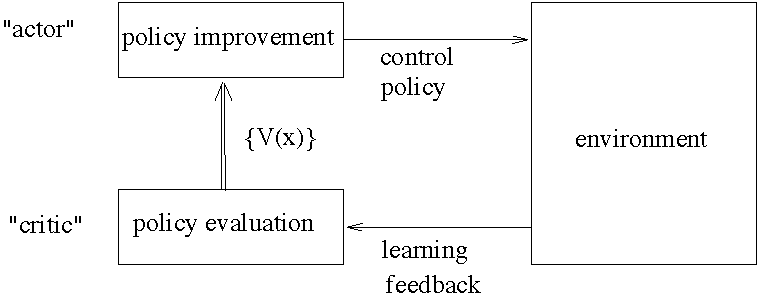
\includegraphics{FIGS/ACRL.pdf}
\end{center}
The ``policy evaluation'' block essentially computes the value function $V^\pi$ under
the current policy (assuming a fixed, stationary policy).
Methods for policy evaluation include:
\begin{enumerate}
  \item ``{Monte Carlo}'' policy evaluation.
  \item Temporal Difference methods - {TD($\la$)}, SARSA, etc.
\end{enumerate}
The ``actor'' block performs some form of policy improvement, based on the
policy iteration idea:
$\bar{\pi} \in \argmax \{r+P^\pi V^\pi\}$.
In addition, it is responsible for implementing some ``exploration'' process.

\item \textbf{Value-Iteration based Schemes:}
These schemes are based on some on-line version of the value-iteration recursions:
$V_{t+1}^* = \max_\pi [r^{\pi}+P^{\pi} V_t^*]$.
The basic learning algorithm in this class is {\em $Q$-learning}.
\end{enumerate}

\section{Example: Deterministic $Q$-Learning}

To demonstrate some key ideas, we start with a simplified learning algorithm
that is suitable for a {\em deterministic} MDP model, namely:
\begin{align*}
& s_{t+1}=f(s_t,a_t) \\
& r_t=r(s_t,a_t)
\end{align*}
We consider the discounted return criterion:
\begin{align*}
V^{\pi}(s) &=\sum_{t=0}^\infty \ga^t r(s_t,a_t)\,,
\quad \text{given } s_0=s, a_t=\pi(s_t)\\
V^*(s) &= \max_\pi V^\pi(s)
\end{align*}
Recall our definition of the $Q$-function (or {\em state-action value function}),
specialized to the present deterministic setting:
$$
Q(s,a)=r(s,a)+\ga V^*(f(s,a))
$$
The optimality equation is then
$$
V^*(s) = \max_a Q(s,a)
$$
or, in terms of $Q$ only:
$$
Q(s,a)=r(s,a)+\ga \max_{a'}Q(f(s,a),a')
$$

Our learning algorithm runs as follows:
\begin{itemize}
\item {\em Initialize:} Set $\hat{Q}(s,a)= Q_0(s,a)$, for all $s$, $a$.
\item At each stage $n=0,1,\dots$:

-- Observe $s_n$, $a_n$, $r_n$, $s_{n+1}$.
% $s\leftarrow s_n$, $a \leftarrow a_n$, $r\leftarrow r_n$, $s'\leftarrow s_{n+1}$.

-- Update $\hat{Q}(s_n,a_n)$:\ \ \
$\hat{Q}(s_n,a_n) := r_n+\ga \max_{a'} \hat{Q}(s_{n+1},a')$
\end{itemize}

We note that this algorithm does not tell us how to choose the actions $a_n$.
The following result is from [Mitchell, Theorem 3.1].

\begin{theorem}[Convergence of $Q$-learning for deterministic MDPs]\ \\
Assume a deterministic MDP model. Let $\hat{Q}_n(s,a)$ denote the estimated
$Q$-function before the $n$-th update.
If each state-action pair is visited \underline{infinitely-often}, then
$\lim_{n\to\infty}\hat{Q}_n(s,a)=Q(s,a)$, for all $(s,a)$.
\end{theorem}

\begin{proof}
Let
$$
\Delta_n \dfn \|\hat{Q}_n-Q\|_\infty = \max_{s,a} |\hat{Q}_n(s,a)-Q(s,a) | \,.
$$
Then at every stage $n$:
\begin{align*}
| \hat{Q}_{n+1}(s_n,a_n)- Q(s_n,a_n)| &= |r_n+\ga\max_{a'} \hat{Q}_n(s_{n+1},a')
- (r_n+\ga\max_{a''} Q(s_{n+1},a'') ) | \\
&= \ga |\max_{a'} \hat{Q}_n(s_{n+1},a') -\max_{a''} {Q}(s_{n+1},a'') | \\
& \le \ga \max_{a'} |\hat{Q}_n(s_{n+1},a') - Q(s_{n+1},a') |
\; \le\;  \ga \Delta_n \,.
\end{align*}
Consider now some interval $[n_1,n_2]$ over which all state-action pairs $(s,a)$
appear at least once. Using the above relation and simple induction, it
follows that $\Delta_{n_2} \le \ga \Delta_{n_1}$. Since $\ga<1$ and since
there is an infinite number of such intervals by assumption, it follows that
$\Delta_n \to 0$.
\end{proof}

\paragraph{Remarks:}
\begin{enumerate}
  \item The algorithm allows the use of an arbitrary policy during learning.
Such an algorithm is called {\em Off-Policy}. In contrast, {\em On-Policy}
algorithms learn the properties of the policy that is actually being applied.
  \item We further note that the ``next-state" $s'=s_{n+1}$ of stage $n$ need not
coincide with the current state $s_{n+1}$ of stage $n+1$. Thus, we may skip
some samples, or even choose $s_n$ at will at each stage. This is a common
feature of off-policy schemes.
  \item A basic requirement in this algorithm is that all state-action pairs will
be sampled "often enough", to ensure that we often use a specific
{\em exploration} algorithm or method. In fact, the speed of convergence
may depend critically on the efficiency of exploration. We shall discuss this
topic in detail further on.
\end{enumerate}

\section{Policy Evaluation: Monte-Carlo Methods}

Policy evaluation algorithms are intended to estimate the value functions
$V^\pi$ or $Q^\pi$ for a given policy $\pi$. Typically these are on-policy
algorithms, and the considered policy is assumed to be stationary (or "almost"
stationary). Policy evaluation is typically used as the ``critic" block of an
actor-critic architecture.

Direct Monte-Carlo methods are the most straight-forward, and are considered
here mainly for comparison with the more elaborate ones. Monte-Carlo methods
are based on the simple idea of averaging a number of random samples of a
random quantity in order to estimate its average.

Let $\pi$ be a fixed stationary policy. Assume we wish to evaluate the
value function $V^\pi$, which is either the discounted return:
$$
V^\pi(s) = E^\pi (\sum_{t=0}^\infty \ga^t r (s_t, a_t) | s_0=s)
$$
or the total return for an SSP (or {\em episodial}) problem:
$$
V^\pi(s) = E^\pi (\sum_{t=0}^T r(s_t, a_t)| s_0=s )
$$
where $T$ is the (stochastic) termination time, or time of arrival to
the terminal state.

Consider first the episodial problem.
Assume that we operate (or simulate) the system with the policy
$\pi$, for which we want to evaluate $V^{\pi}$.
Multiple trials may be performed, starting from arbitrary initial conditions,
and terminating at $T$ (or truncated before).

After visiting state $s$, say at time $t_s$, we add-up the total cost until the
target is reached:
$$
\hat v(s) = \sum_{t=t_s}^T R_t\,.
$$
After $k$ visits to $s$, we have a sequence of total-cost estimates:
$$
\hat v_1 (s) , \cdots, \hat v_k (s)\,.
$$
We can now compute our estimate:
$$
\hat V_k(s) = \frac{1}{k} \sum_{i=1}^k \hat v_i (s)\,.
$$
By repeating these procedure for all states,
we estimate $V^{\pi}(\cdot)$.

\paragraph{State counting options:} Since we perform multiple trials and
each state can be visited several times per trial, there are several options
regarding the visits that will be counted:
\begin{itemize} \negspace
\item[a.]
Compute $\hat V(s)$ only for initial states $(s_0=s)$.
\item[b.]
Compute $\hat V(s)$ each time $s$ is visited.
\item[c.]
Compute $\hat V(s)$ only on first visit of $s$ at each trial.
\end{itemize} \negspace
Method (b) gives the largest number of samples, but
these may be correlated (hence, lead to non-zero bias for finite times).
But in any case, $\hat V_k(s) \to V^{\pi}(s)$ is guaranteed as $k\to\infty$.
Obviously, we still need to guarantee that each state is visited enough
-- this depends on the policy $\pi$ and our choice of initial conditions
for the different trials.

\paragraph{Remarks:}
\begin{enumerate}
  \item The explicit averaging of the $\hat v_k$'s may be replaced by
the iterative computation:
$$
\hat V_k(s) = \hat V_{k-1} (s) + \al_k
\Bigl[\hat v_k (s) - \hat V_{k-1} (s) \Bigr] \,,
$$
with $\al_k=\frac{1}{k}$.  Other choices for $\al_k$ are also common,
e.g.\ $\al_k = \frac{\ga}{k}$, and $\al_k=\eps$
(non-decaying gain, suitable for non-stationary conditions).
  \item For discounted returns, the computation needs to be truncated at some
finite time $T_s$, which can be chosen large enough to guarantee a small
error:
$$
\hat v(s) = \sum_{t=t_s}^{T_s} (\ga)^{t-t_s} R_t\,.
$$
\end{enumerate}

\section{Policy Evaluation: Temporal Difference Methods}

\subsection{The TD(0) Algorithm}\label{ss:TD0}

Consider the total-return (SSP) problem with $\ga=1$.
Recall the fixed-policy Value Iteration procedure of Dynamic Programming:
$$
V_{n+1}(s) = E^{\pi} (r(s,a) + V_n(s') )
           = r(s,\pi(s)) + \sum_{s'} p(s' | s,\pi(s)) V_n(s')\,,\quad \forall s\in S,
$$
or $V_{n+1}  = r^{\pi} + P^{\pi} V_n$, which converges to $V^{\pi}$.

Assume now that $r^{\pi}$ and $P^{\pi}$ are not given.
We wish to devise a ``learning version" of the above policy iteration.

Let us run or simulate the system with policy $\pi$.
Suppose we start with some estimate $\hat V$ of $V^{\pi}$.
At time $n$, we observe $s_n$, $r_n$ and $s_{n+1}$.
We note that $[r_n + \hat V(s_{n+1})]$ is an unbiased
estimate for the right-hand side of the value iteration equation,
in the sense that
$$
E^\pi (r_n + \hat V(s_{n+1}) | s_n) =
r(s_n,\pi(s_n)) + \sum_{s'} p(s' | s_n,\pi(s_n)) V_n(s')
$$
However, this is a {\em noisy} estimate, due to randomness in $r$ and $s'$.
We therefore use it to modify $\hat V$ only slightly, according to:
\begin{align*}
\hat V (s_n) & := (1-\al_n) \hat V(s_n) + \al_n [r_n + \hat V (s_{n+1}) ] \\
& = \hat V(s_n) + \al_n [r_n + \hat V(s_{n+1}) - \hat V(s_n)]
% \underbrace{[r_n + \hat V(s_{n+1}) - \hat V(s_n)]}_{\bydef d_n}
\end{align*}
Here $\al_n$ is the {\em gain} of the algorithm.
If we define now
$$
d_n \dfn r_n + \hat V(s_{n+1}) - \hat V(s_n)
$$
we obtain the update rule:
$$
\hat V (s_n) := \hat V(s_n)+\al_n d_n \,
$$

$d_n$ is called the {\em Temporal Difference}.
The last equation defines the \underline{TD(0) algorithm}.



Note that $\hat V(s_n)$ is updated on basis of $\hat V(s_{n+1})$, which is
itself an estimate.  Thus, TD is a ``bootstrap" method: convergence of
$\hat V$ at each states $s$ is inter-dependent with other states.

\paragraph{Convergence results for TD(0)\quad (preview):}
\begin{enumerate}
\item
If $\al_n \searrow 0 $ at suitable rate ($\al_n \approx 1/$no.~of visits to
$s_n$), and each state is visited i.o., then
$\hat V_n \to V^{\pi}$ w.p. 1.

\item
If $\al_n= \al_0$ (a small positive constant) and each state is visited i.o.,
then $\hat V_n$ will ``eventually'' be close to $V^{\pi}$ with high probability.
That is, for every $\eps>0$ and $\delta>0$ there exists $\al_0$ small enough so that
$$
\lim_{n\to\infty}
\mbox{\rm Prob}(|\hat V_n - V^{\pi} | > \eps) \le \delta \,.
$$
\end{enumerate}

\subsection{TD with $\ell$-step look-ahead}

TD(0) looks only one step in the ``future'' to update $\hat V(s_n)$,
based on $r_n$ and $\hat V(s_{n+1})$.  Subsequent changes will not affect $\hat
V(s_n)$ until $s_n$ is visited again.

Instead, we may look $\ell$ steps in the future, and replace $d_n$ by
\begin{align*}
d_n^{(\ell)} & \dfn \sum_{m=0}^{\ell-1} r_{n+m} + \hat
V(s_{n+\ell}) -
\hat V(s_n) \\
& = \sum_{m=0}^{\ell-1} d_{n+m}
\end{align*}
where $d_n$ is the one-step temporal difference as before.
The iteration now becomes
$$\hat V(s_n) := \hat V(s_n) + \al_n d_n^{(\ell)}.$$

This is a ``middle-ground'' between TD(0) and Monte-Carlo evaluation!


\subsection{The TD($\la$) Algorithm}

Another way to look further ahead is to consider all future Temporal
Differences with a ``fading memory'' weighting:
\begin{equation}
\label{*}
\hat V(s_n) := \hat V(s_n) + \al ( \sum_{m=0}^\infty \la^m d_{n+m} )
\end{equation}
where $0 \le \la \le 1$.
For $\la=0$ we get TD(0); for $\la=1$ we obtain the Monte-Carlo sample!

Note that each run is terminated when the terminal state is reached,
say at step $T$. We thus set $d_n\equiv 0$ for $n\ge T$.

The convergence properties of TD($\la$) are similar to TD(0).
However, TD($\la$) often converges faster than TD(0) or
direct Monte-Carlo methods, provided that $\la$ is properly chosen.
This has been experimentally observed, especially when function
approximation is used for the value function.

\paragraph{Implementations of TD($\la$):}

There are several ways to implement the relation in (\ref{*}).
\begin{enumerate}
  \item Off-line implementation: $\hat V$ is updated using (\ref{*})
at the end of each simulation run, based on the
stored $(s_t, d_t)$ sequence from that run.

  \item Each $d_n$ is used as soon as becomes available, via the following
backward update (also called ``on-line implementation''):
\begin{equation}
\label{**}
\hat V(s_{n-m}) := \hat V(s_{n-m}) + \al \cdot \la^m d_n\,, \qquad m=0,\dots,n\,.
\end{equation}
This requires only keeping track of the state sequence $(s_t, t \ge 0)$.
Note that if some state $s$ appears twice in that sequence, it is updated
twice.
  \item Eligibility-trace implementation:
\begin{equation} \label{TDL1}
\hat V(s) := \hat V(s) + \al d_n e_n (s)\,, \qquad s\in S
\end{equation}
where
$$
e_n (s) = \sum_{k=0}^n \la^{n-k} 1\{s_k = s\}
$$
is called the {\em eligibility trace} for state $s$.

The eligibility trace variables $e_n (s)$ can also be computed recursively.
Thus, set $e_0(s)=0 \quad \forall s$, and
\begin{equation} \label{TDL2}
e_n(s) := \la e_{n-1}(s) +1\{s_n=s\} \,=\, \left\{
\begin{array}{lll}
\la\cdot e_{n-1}(s) + 1 & \text{if} & s=s_n \\
\la\cdot e_{n-1}(s)  & \text{if} & s\not=s_n
\end{array}
\right.
\end{equation}
Equations (\ref{TDL1}) and (\ref{TDL2}) provide a fully recursive implementation
of TD($\la$).
\end{enumerate}

\subsection{TD Algorithms for the Discounted Return Problem}

For $\ga$-discounted returns, we obtain the following equations for the
different TD algorithms:
\begin{enumerate}
  \item TD(0):
\begin{align*}
\hat V(s_n) & := (1-\al) \hat V(s_n) + \al [ r_n +
\ga\hat V (s_{n+1})] \\
& = \hat V (s_n) + \al \cdot d_n,
\end{align*}
with $d_n \dfn r_n + \ga V (s_{n+1}) - V(s_n)$.

  \item $\ell$-step look-ahead:
\begin{align*}
\hat V(s_n) & := (1-\al) \hat V(s_n) + \al [r_n + \ga r_{n+1}
+ \cdots + \ga^\ell V_{n+\ell}] \\
& = \hat V(s_n) + \al [d_n + \ga d_{n+1} + \cdots +
\ga^{\ell-1} d_{n+\ell-1}]
\end{align*}
  \item TD($\la$):
$$
\hat V(s_n) := \hat V (s_n) + \al \sum_{k=0}^\infty (\ga \la )^k
d_{n+k}\,.
$$
The eligibility-trace implementation is:
\begin{align*}
& \hat V(s) := \hat V(s) + \al d_n e_n (s) \,, \\
& e_n(s) := \ga\la e_{n-1}(s) +1\{s_n=s\} \,.
\end{align*}
\end{enumerate}

\subsection{Q-functions and their Evaluation}\label{ss:Q_eval}

For policy improvement, what we require is actually the
$Q$-function $Q^{\pi}(s,a)$, rather than $V^{\pi}(s)$.
Indeed, recall the policy-improvement step of policy iteration, which defines
the improved policy $\hat\pi$ via:
$$
\hat \pi(s) \in \argmax_a \{r(s,a) + \ga \sum_{s'} p(s'|s,a) V^{\pi} (s') \}
 \equiv \argmax_a Q^{\pi}(s,a)\,.
$$
How can we estimate $Q^{\pi}$?

\paragraph{1. Using $\hat V^{\pi}$:}
If we know the one-step model parameters $r$ and $p$,
we may estimate $\hat V^{\pi}$ as above and compute
$$
\hat Q^{\pi} (s,a) \bydef r(s,a) +\ga \sum p(s'|s,a) \hat V^{\pi}(s')\,.
$$
When the model is not known, this requires to estimate $r$ and $p$ on-line.

\paragraph{2. Direct estimation of $Q^{\pi}$:}
This can be done using the same methods as outlined for $\hat V^{\pi}$,
namely Monte-Carlo or TD methods. We mention the following:

\paragraph{The SARSA algorithm:} This is the equivalent of TD(0).
At each stage we observe $(s_n,a_n,r_n,s_{n+1},a_{n+1})$, and update
\begin{align*}
Q(s_n, a_n) & := Q(s_n,a_n) + \al_n \cdot d_n \\
d_n & = r_n +  \ga Q(s_{n+1}, a_{n+1}) - Q(s_n, a_n), \mbox{where } a_{n+1}=\pi(s_{n+1}).
\end{align*}
Similarly, the SARSA($\la$) algorithm uses
\begin{align*}
Q(s, a) & := Q(s,a) + \al_n(s,a) \cdot d_n e_n(s,a) \\
\quad e_n(s,a)& := \ga \la e_{n-1}(s,a)+1\{s_n=1,a_n=a\} \,.
\end{align*}

Note that:\\
-- The estimated policy $\pi$ must be the one used (``on-policy'' scheme).\\
-- More variables are estimated in $Q$ than in $V$.




\section{Policy Improvement}

Having studied the ``policy evaluation'' block of the actor/critic scheme, we
turn to the policy improvement part.

Ideally, we wish to implement policy iteration through learning:
\begin{itemize} \negspace
\item[(i)]
Using policy $\pi$, evaluate $\hat Q \approx Q^{\pi}$.  Wait for convergence.
\item[(ii)]
Compute $\hat \pi = \argmax \hat Q$ (the ``greedy policy'' w.r.t. $\hat Q$).
\end{itemize}

\paragraph{Problems:}
\begin{itemize}
\item[a.]
Convergence in (i) takes infinite time.
\item[b.]
Evaluation of $\hat Q$ requires trying all actions -- typically requires
an exploration scheme which is richer than the current policy $\pi$.
\end{itemize}

To solve (a), we may simply settle for a finite-time estimate of $Q^{\pi}$, and
modify $\pi$ every (sufficiently long) finite time interval.
A more ``smooth" option is to modify $\pi$ slowly in the ``direction'' of the
maximizing action. Common options include:
\begin{itemize}
\item[(i)]
Gradual maximization:
If $a^*$ maximizes $\hat Q(s,a)$, where $s$ is the state currently examined,
then set
$$
\left\{
\begin{array}{l}
\pi(a^*|s) := \pi(a^*|s) + \al \cdot [1-\pi(a^*|s)]\\
\pi(a|s) := \pi(a|s) - \al \cdot \pi(a|s), \quad a\not= a^*\,.
\end{array}
\right.
$$
Note that $\pi$ is a {\em randomized} stationary policy,
and indeed the above rule keeps $\pi(\cdot |s)$ as a probability vector.
\item[(ii)]
Increase probability of actions with high $Q$: Set
$$
\pi(a|s)=\frac{e^{\beta(s,a)}}{\sum_{a'} e^{\beta(s,a')}}
$$
(a Boltzmann-type distribution), where $\beta$ is updated as follows:
$$
\beta(s,a):=\beta(s,a) +\alpha[\hat Q(s,a)- \hat Q(s,a_0)].
$$
Here $a_0$ is some arbitrary (but fixed) action.
\item[(iii)]
``Pure" actor-critic: Same Boltzmann-type distribution is used, but now with
$$
\beta(s,a):=\beta(s,a) +\alpha[r(s,a)+\gamma\hat V(s') -\hat V(s)]
$$
for $(s,a,s')=(s_n,a_n,s_{n+1})$. Note that this scheme uses directly
$\hat V$ rather than $\hat Q$. However it is more noisy and harder to
analyze than other options.
\end{itemize}

To address problem (b) (exploration), the simplest approach is to superimpose
some randomness over the policy in use.
Simple local methods include:
\begin{itemize}
\item[(i)]
$\epsilon$-exploration: Use the nominal action $a_n$ (e.g., $a_n=\argmax_a Q(s_n,a)$)
with probability $(1-\epsilon)$, and otherwise (with probability $\epsilon$) choose
another action at random. The value of $\epsilon$ can be reduced over time,
thus shifting the emphasis from exploration to exploitation.
\item[(ii)]
Softmax: Actions at state $s$ are chosen according to the probabilities
$$
\pi(a|s) = \frac{e^{Q(s,a)/\theta}}{\sum_a e^{Q(s,a)/\theta}}\,.
$$
$\theta$ is the ``temperature" parameter, which may be reduced gradually.
\item[(iii)]
The above ``gradual maximization'' methods for policy improvement.
\end{itemize}
These methods however may give slow convergence results, due to their local
(state-by-state) nature.

Another simple (and often effective) method for exploration relies
on the principle of {\em optimism in the face of uncertainty}.
For example, by initializing $\hat Q$ to high (optimistic) values,
we encourage greedy action selection to visit unexplored
states. %We will revisit those ideas later on in the course.



Convergence analysis for actor-critic schemes is relatively hard.
Existing results rely on a {\em two time scale} approach, where
the rate of policy update is assumed much slower than the
rate of value-function update.



\section{Q-learning}

$Q$-learning is the most notable representative of
{\em value iteration} based methods.
Here the goal is to compute directly the {\em optimal} value function.
These schemes are typically {\em off-policy} methods -- learning
the optimal value function can take place under any policy (subject to
exploration requirements).

Recall the definition of the (optimal) $Q$-function:
$$
Q(s,a) \dfn r(s,a) + \ga \sum_{s'} p(s'|s,a) V^* (s')\,.
$$
The optimality equation is then $V^*(s)=\max_a Q(s,a)\,,\; s\in S$,
or in terms of $Q$ only:
$$
Q(s,a) = r(s,a) + \ga \sum_{s'} p(s' |s,a) \max_{a'} Q(s',a')\,,\quad
s\in S, a\in A \,.
$$
The value iteration algorithm is given by:
$$
V_{n+1}(s) = \max_a \{ r(s,a) +  \ga \sum_{s'} p(s'|s,a) V_n (s') \}\,, \quad s\in S
$$
with $V_n\to V^*$. This can be reformulated as
\begin{equation}
\label{star} Q_{n+1} (s,a) = r(s,a) +\ga \sum_{s'} p(s'|s,a)
\max_{a'} Q_n (s',a')\,,
\end{equation}
with $Q_n\to Q$.

We can now define the on-line (learning) version of the $Q$-value iteration
equation.

\paragraph{The $Q$-learning algorithm:}

-- initialize $\hat Q$.

-- At stage $n$: Observe $(s_n,a_n,r_n,s_{n+1})$, and let
\begin{align*}
\hat Q(s_n,a_n) & := (1-\al_n) \hat Q (s_n,a_n) + \al_n [r_n + \ga \max_{a'} \hat {Q}
(s_{n+1}, a') ] \\
& = \hat {Q} (s_n,a_n) + \al_n [r_n + \ga \max_{a'} \hat {Q} (s_{n+1},a')
- \hat{Q} (s_n,a_n)]
\,.
\end{align*}

The algorithm is obviously very similar to the basic TD schemes for policy evaluation,
except for the maximization operation.

\medskip
\paragraph{Convergence:}
If all $(s,a)$ pairs are visited i.o., and $\al_n\searrow 0$ at appropriate
rate, then $\hat Q_n \to Q^*$.

\paragraph{Policy Selection:}
\begin{itemize} \negspace
\item[--]
Since learning the $Q^*$ does not depend on optimality of the policy used, we
can focus on exploration during learning. However, if learning takes place
while the system is in actual operation, we may still need to use a
close-to-optimal policy, while using the standard exploration techniques
($\eps$-greedy, softmax, etc.).
\item[--]
When learning stops, we may choose a greedy policy:
$$
\hat \pi(s) = \max_a \hat Q(s,a)\,.
$$
\end{itemize}

\paragraph{Performance:}
$Q$-learning is very convenient to understand and implement; however,
convergence may be slower than actor-critic (TD($\lambda$)) methods,
especially if in the latter we only need to evaluate $V$ and  not $Q$.

% } large ended
%
%\end{document}
%~

\section{Exercises}

\begin{exercise}[\textbf{The $c \mu$ rule revisited}]
Consider again the job processing domain of Exercise \ref{ex:c_mu}:

$N$ jobs are scheduled to run on a single server. At each time step $(t=0,1,2,�)$, the sever may choose one of the remaining unfinished jobs to process. If job $i$ is chosen, then with probability ${\mu _i} > 0$ it will be completed, and removed from the system; otherwise the job stays in the system, and remains in an unfinished state. Notice that the job service is memoryless - the probability of a job completion is independent of the number of times it has been chosen.
Each job is associated with a waiting cost ${c_i} > 0$ that is paid for each time step that the job is still in the system. The server's goal is minimizing the total cost until all jobs leave the system.

This time, we will solve the problem numerically, testing the various dynamic programming and reinforcement learning algorithms we have learned so far.

We consider the following specific case, with $N = 5$:

\begin{center}
\begin{tabular}{|l|l|l|l|l|l|}
\hline
{\bf $i$}  & {\bf 1} & {\bf 2} & {\bf 3} & {\bf 4} & {\bf 5} \\ \hline
${\mu _i}$ & 0.6     & 0.5     & 0.3     & 0.7     & 0.1     \\ \hline
${c_i}$    & 1       & 4       & 6       & 2       & 9       \\ \hline
\end{tabular}
\end{center}

\paragraph{Part 1 - Planning}
In this part all the Matlab functions may use the true model (i.e., the ${\mu _i}$'s and ${c_i}$'s).
\begin{enumerate}
  \item How many states and actions are in the problem?
\end{enumerate}  
  Let $S$ denote the state space. A deterministic policy $\pi $ is a mapping from states to actions. In our case, it will be represented in Matlab as a vector of length $|S|$, in which each element denotes the selected action ($1, \ldots ,N$) for the corresponding state.
\begin{enumerate} 
\setcounter{enumi}{1} 
  \item Write a function (in Matlab) that take as input a policy, and returns the corresponding value function ${V^\pi }$, also represented as a vector of length $|S|$. You can solve it either directly by matrix inversion, or iteratively. Remember that the value of the terminal state (no more jobs left) is zero by definition.
  \item Plot the values of the policy ${\pi _c}$ that selects the job with the maximal cost ${c_i}$, from the remaining unfinished jobs.
  \item Write a function that calculates the optimal policy ${\pi ^*}$ using the policy iteration algorithm, and execute it, starting from the initial policy ${\pi _c}$. For each iteration of the algorithm, plot the value of the initial state ${s_0}$ (no jobs completed) for the current policy. How many steps are required for convergence?
  \item Compare the optimal policy ${\pi ^*}$ obtained using policy iteration to the $c\mu $ law. Also plot ${V^{{\pi ^*}}}$ vs. ${V^{{\pi _c}}}$.
  \item Write a simulator of the problem: a function that takes in a state $s$ and action $a$, and returns the cost of the state $c(s)$, and a random next state $s'$, distributed according to the transition probabilities of the problem.
\end{enumerate}

\paragraph{Part 2 - Learning}
In this part the learning algorithms cannot use the true model parameters, but only have access to the simulator function written above.

\begin{enumerate}
\setcounter{enumi}{6}
  \item \textbf{Policy evaluation:} consider again the policy ${\pi _c}$, and use the TD(0) algorithm to learn the value function ${V^{{\pi _c}}}$. Start from ${\hat V_{TD}}(s) = 0$ for all states. Experiment with several step size ${\alpha _n}$ schedules:
      \begin{enumerate}
        \item ${a_n} = 1/\left( {no.\,of\,visits\,to\,{s_n}} \right)$
        \item ${a_n} = 0.01$
        \item ${a_n} = \frac{{10}}{{100 + \left( {no.\,of\,visits\,to\,{s_n}} \right)}}$
      \end{enumerate}
For each step-size schedule, plot the errors ${\left\| {{V^{{\pi _c}}} - {{\hat V}_{TD}}} \right\|_\infty }$ and $\left| {{V^{{\pi _c}}}({s_0}) - {{\hat V}_{TD}}({s_0})} \right|$ as a function of iteration $n$. Explain the motivation behind each step-size schedule, and how it reflects in the results.

  \item Now, run policy evaluation using TD($\lambda $). Choose your favorite step-size schedule, and plot the errors ${\left\| {{V^{{\pi _c}}} - {{\hat V}_{TD}}} \right\|_\infty }$ and $\left| {{V^{{\pi _c}}}({s_0}) - {{\hat V}_{TD}}({s_0})} \right|$ as a function of iteration $n$ for several choices of $\lambda $. Repeat each experiment $20$ times and display average results.
  \item \textbf{Q-learning:} run Q-learning to find the optimal policy. Start from $\hat Q(s,a) = 0$ for all states and actions. Experiment with the 3 previous step-size schedules. Use $\epsilon$-greedy exploration, with $\epsilon = 0.1$.
      
      For some $\hat Q$, let  ${\pi _{\hat Q}}$ denote the greedy policy w.r.t. $\hat Q$, i.e., ${\pi _{\hat Q}}(s) = \arg {\min _a}\hat Q(s,a)$.
      
For each step-size schedule, plot the errors ${\left\| {{V^*} - {V^{{\pi _{\hat Q}}}}} \right\|_\infty }$ and $\left| {{V^*}({s_0}) - \arg {{\min }_a}\hat Q({s_0},a)} \right|$ as a function of iteration $n$. You may use the policy evaluation function you wrote in (2) to calculate ${V^{{\pi _{\hat Q}}}}$. If this step takes too long, you may plot the errors only for $n = 100,200,300,...$ etc.

  \item Repeat the previous Q-learning experiment for your favorite step-size schedule but now with $\epsilon = 0.01$. Compare.
\end{enumerate}
\end{exercise}



\chapter{The Stochastic Approximation Algorithm}
%%chapter 6 (now 5), SA, by Lesley, modified 12.02
%% unified with "Stochastic Processes" on 4/2011.
%
%\input{header}
%
%\begin{document}
%
%% First page number
%\setcounter{page}{1}
%% PREVIOUS section number
%\setcounter{section}{4}
%% PREVIOUS subsection number
%\setcounter{subsection}{0}
%
%% ***********************************************************************
%\textsc{Reinforcement Learning \hfill Spring 2015$\;$ \\
%Lecture Notes \hfill Shie Mannor and Nahum Shimkin}
%\vspace{-18pt}
%\par
%\hrulefill
%% ***********************************************************************
%
%
%% {\large
%
%\section{The Stochastic Approximation Algorithm}

\newcommand{\midarrow}{\to}
\newcommand{\uu}{\underline}
\newcommand{\oo}{\overline}
\newcommand{\limn}{\lim_{n \to \infty}}
\newcommand{\limsupn}{\limsup_{n \to \infty}}

\section{Stochastic Processes -- Some Basic Concepts}

\subsection{Random Variables and Random Sequences}

Let $(\Omega,\cF,P)$ be a probability space, namely:
\begin{itemize}
\item[--] $\Omega$ is the sample space.
\item[--] $\cF$ is the event space. Its elements are subsets
of $\Omega$, and it is required to be a $\sigma$-algebra
(includes $\emptyset$ and $\Omega$; includes all countable union of its members;
includes all complements of its members).
\item[--]$P$ is the probability measure (assigns a probability in [0,1] to each element
of $\cF$, with the usual properties: $P(\Omega)=1$, countably additive).
\end{itemize}

A random variable (RV) $X$ on $(\Omega,\cF)$
is a function $X:\Omega \to \reals$, with values $X(\omega)$.
It is required to be {\em measurable} on $\cF$,
namely, all sets of the form $\{\omega: X(\omega)\le a\}$ are
events in $\cF$.

A vector-valued RV is a vector of RVs. Equivalently, it is a
function $X:\Omega \to \reals^d$, with similar measurability requirement.

A {\em random sequence}, or a discrete-time {\em stochastic process},
is a sequence $(X_n)_{n\ge 0}$ of
$\reals^d$-valued RVs, which are all defined on the same probability space.

\subsection{Convergence of Random Variables}

A random sequence may converge to a random variable, say to $X$.
There are several useful notions of convergence:
\begin{enumerate}
\item
Almost sure convergence (or: convergence with probability 1):
$$
X_n \midarrow{a.s.}X  \quad \text{if} \quad P \{\lim_{n\to\infty} X_n =X \} = 1 \,.
$$
\item
Convergence in probability:
$$
X_n \midarrow{p} X \quad \text{if} \quad
\lim_{n\to\infty} P (|X_n - X| > \epsilon) =0\,,
\forall \epsilon >0\,.
$$
\item
Mean-squares convergence (convergence in $L^2$):
$$
 X_n \midarrow{L^2} X
\quad \text{if} \quad
E |X_n - X_\infty|^2 \to 0 \,.$$
\item
Convergence in Distribution:
$$ \text{$X_n \midarrow{Dist} X$ (or $X_n \Rightarrow X$)}
\quad \text{if} \quad
Ef(X_n) \to Ef(X)$$
for every bounded and continuous function $f$.
\end{enumerate}

\medskip

The following relations hold:
\begin{itemize}
\item[a.]
Basic implications: \ \ \
(a.s. or $L^2$) $\Longrightarrow$ $p$ $\Longrightarrow$ Dist
\item[b.]
Almost sure convergence is equivalent to
$$
\lim_{n\to\infty} P \{\sup_{k\geq n} |X_k - X| > \epsilon) = 0 \,,
\quad \forall \epsilon >0\,.
$$
\item[c.] A useful {\em sufficient} condition for a.s.\  convergence:
$$
\sum_{n=0}^{\infty} P(|X_n-X| > \eps) < \infty \,.
$$
\end{itemize}

\subsection{Sigma-algebras and information}

Sigma algebras (or $\sigma$-algebras) are part of the mathematical structure of
probability theory.
They also have a convenient interpretation as ''information sets", which
we shall find useful.

\begin{itemize}
\item
Define $\cF_X\dfn \sigma\{X\}$, the $\sigma$-algebra generated by the RV $X$.
This is the smallest $\sigma$-algebra that contains all sets of the
form $\{X\leq a\} \equiv \{\omega\in\Omega: X(\omega) \leq a\}$.
\item
We can interpret $\sigma\{X\}$ as carrying all the information in
$X$. Accordingly, we identify
$$
E(Z | X) \equiv E(Z | \cF_X)\,.
$$
Also, ``$Z$ is measurable on $\sigma\{X\}$"  is equivalent to:
$Z=f(X)$ (with the additional technical requirement that $f$ is a
Borel measurable function).
\item
We can similarly define $\cF_n = \sigma\{X_1,\dots, X_n\}$, etc. Thus,
$$
E(Z | X_1,\dots,X_n) \equiv E(Z | \cF_n)\,.
$$
\item
Note that $\cF_{n+1} \supset \cF_n$: more RVs carry more information,
leading $\cF_{n+1}$ to be finer, or ``more detailed"
\end{itemize}

\subsection{Martingales}
A \emph{martingale} is defined as follows.
\begin{definition}[\textbf{Martingale}]
A sequence $(X_k, \cF_k)_{k\ge 0}$
on a given probability space $(\Omega,\cF, P)$
is a martingale if
\begin{itemize}
\item[a.]
$(\cF_k)$ is a ``filtration'' -- an increasing sequence of
$\sigma$-algebras in $\cF$.
\item[b.]
Each RV  $X_k$ is $\cF_k$-measurable.
\item[c.]
$E(X_{k+1} | \cF_k) = X_k$\ \  (P--a.s.).
\end{itemize}
\end{definition}
\paragraph{Note:}
\begin{itemize}
\item
(a) Property is roughly equivalent to:\\
\hspace*{2cm}$\cF_k$ represents (the information in)
some RVs $(Y_0, \ldots, Y_k)$,
\\
and (b) then means:\ \
$X_k$  is a function of $(Y_0, \ldots, Y_k)$.
\item
A particular case is $\cF_n=\sigma\{X_1,\dots,X_n\}$
\ (a self-martingale).
\item
The central property is (c), which says that the conditional mean
of $X_{k+1}$ equals $X_k$. This is obviously
stronger than  $E(X_{k+1})=E(X_k)$.
\item
The definition sometimes requires also that $E|X_n|<\infty$,
we shall assume that below.
\item
Replacing (c) by $E(X_{k+1} | \cF_k) \geq X_k$ gives a {\em submartingale},
while $E(X_{k+1} | \cF_k) \leq X_k$ corresponds to a {\em supermartingale}.
\end{itemize}

\paragraph{Examples:}
\begin{itemize}
\item[a.]
The simplest {example} of a martingale is
$$
X_k = \sum_{\ell=0}^k \xi_\ell\,,
$$
with $\{\xi_k\}\;$ a sequence of 0-mean independent RVs, and
$\cF_k= \sigma (\xi_0, \ldots, \xi_k)$.
\item[b.]
$X_k=E(X|\cF_k)$, where $(F_k)$ is a given filtration and $X$ a fixed RV.
\end{itemize}

Martingales play an important role in the convergence analysis of
stochastic processes. We quote a few basic theorems
(see, for example: A.N. Shiryaev, {\it Probability,} Springer, 1996).

\begin{theorem}[\textbf{Martingale Inequalities}]

Let$(X_k, \cF_k)_{k\ge 0}$ be a martingale. Then for every $\la>0$ and $p\ge 1$
$$
P\left\{ \max_{k\le n} |X_k| \ge \la \right\} \le \frac{E |X_n|^p}{\la^p},
$$
and for $p>1$
$$
% E\left[(\max_{k\le n}|X_k|)^p \right] \le \textstyle{(\frac{p}{p-1})^p} E(|X_n|^p) \,.
E[(\max_{k\le n}|X_k|)^p ] \le \textstyle{(\frac{p}{p-1})^p} E(|X_n|^p) \,.
$$
\end{theorem}

\paragraph{Martingale Convergence Theorems}
\begin{theorem}[\textbf{Convergence with Bounded-moments}] Consider a martingale $(X_k, \cF_k)_{k\ge 0}$.
Assume that:\\
\hspace*{1in} $E|X_k|^q \le C$ for some $C<\infty$, $q \ge 1$ and all $k$.\\
Then
$\{X_k\}$ converges (a.s.) to a RV $X_\infty$ (which is finite w.p.\  1).
\end{theorem}
\begin{theorem}[\textbf{Positive Martingale Convergence}] If $(X_k, \cF_k)$ is
a \uu{positive}
martingale (namely $X_n \ge 0$), then $X_k$ converges (a.s.) to some RV $X_\infty$.
\end{theorem}

\begin{definition}[\textbf{Martingale Difference}]
The sequence $(\xi_k, \cF_k)$ is a {\em martingale difference} sequence if
property (c) is replaced by $E(\xi_{k+1}| \cF_k) = 0$.
\end{definition}
In this case we have:
\begin{theorem}[\textbf{Martingale Difference Convergence}] Suppose that for some $0 < q \le 2$,
$\sum_{k=1}^\infty \frac{1}{k^q} E (|\xi_k|^q | F_{k-1}) < \infty$ (a.s.).
Then $\limn \frac{1}{n} \sum_{k=1}^n \xi_k = 0$ (a.s.).
\end{theorem}

For example, the conclusion holds if the sequence $(\xi_k)$ is bounded,
namely $|\xi_k| \le C$ for some $C>0$ (independent of $k$).


\paragraph{Note:}
\begin{itemize}
\item
It is trivially seen that $(\xi_n\dfn X_n-X_{n-1})$ is a martingale difference
if $(X_n)$ is a martingale.
\item
More generally, for any sequence $(Y_k)$ and filtration $(\cF_k)$, where
$Y_k$ is measurable on $\cF_k$,
the following is a martingale difference:
$$
\xi_k \triangleq Y_k - E(Y_k | \cF_{k-1})\,.
$$
The conditions of the last theorem hold for this $\xi_k$ if either:\\
(i) $|Y_k | \le M$ $\forall k$ for some constant $M < \infty$,\\
(ii) or, more generally, $E(|Y_k|^q | \cF_{k-1}) \le M$ (a.s.) for some $q>1$ and
a finite RV $M$.\\
In that case we have
$$
\frac{1}{n} \sum_{k=1}^n \xi_k \,\equiv\, \frac{1}{n}
\sum_{k=1}^n ( Y_k - E (Y_k | \cF_{k-1})) \to 0 \quad \text{(a.s.)}
$$
\end{itemize}


\section{The Basic SA Algorithm}

The stochastic approximations (SA) algorithm essentially solves a system
of (nonlinear) equations of the form
$$
h(\theta) = 0,
$$
based on noisy measurements of $h(\theta)$.

More specifically, we consider a (continuous) function $h: \reals^d \to \reals^d$,
with $d\ge 1$, which depends on a set of parameters $\theta \in\reals^d$.
Suppose that $h$ is unknown. However, for each $\theta$  we can measure
$Y= h(\theta) + \om$, where $\om$ is some $0$-mean noise.
The classical SA algorithm (Robbins-Monro, 1951) is of the form
\begin{align*}
\theta_{n+1} & = \theta_n + \alpha_n Y_n \\
& = \theta_n + \alpha_n[h(\theta_n)
+ \om_n], \quad n \ge 0\,.
\end{align*}
Here $\alpha_n$ is the algorithm the step-size, or {\em gain}.

Obviously, with zero noise ($\om_n\equiv 0$) the stationary points of the algorithm
coincide with the solutions of $h(\theta)=0$.
Under appropriate conditions (on $\alpha_n$, $h$ and $\om_n$) the algorithm
indeed can be shown to converge to a solution of $h(\theta)=0$.

\paragraph{References:
}\begin{enumerate}
  \item H.~Kushner and G.~Yin, {\em Stochastic Approximation Algorithms and Applications},
Springer, 1997.

  \item V. Borkar, {\em Stochastic Approximation: A Dynamic System Viewpoint}, Hindustan, 2008.

  \item J. Spall, {\em Introduction to Stochastic Search and Optimization: Estimation, Simulation
and Control}, Wiley, 2003.
\end{enumerate}

\paragraph{Some examples of the SA algorithm:}

\begin{itemize}
\item[a.]
{\em Average of an i.i.d.\ sequence:}
Let $(Z_n)_{\ge 0}$ be an i.i.d.\  sequence with mean $\mu = E(Z_0)$ and
finite variance.  We wish to estimate the mean.

The iterative algorithm
$$
\theta_{n+1} = \theta_n + \frac{1}{n+1} [Z_n - \theta_n]
$$
gives
$$
\theta_n = \frac{1}{n} \theta_0 + \frac{1}{n} \sum_{k=0}^{n-1} Z_k \to
\mu \text{\ \ (w.p.~1),\ \ \ by the SLLN} .
$$
This is a SA iteration, with $\alpha_n=\frac{1}{n+1}$, and
$Y_n = Z_n - \theta_n$.
% = (\mu - \theta_n) + (Y_n-\mu).
Writing $Z_n=\mu+\om_n$ ($Z_n$ is considered a noisy measurement of $\mu$,
with zero-mean noise $\om_n$), we can identify
$h(\theta) = \mu - \theta$.

\item[b.]
{\em Function minimization:} Suppose we wish to minimize a (convex) function $f(\theta)$.
Denoting $h(\theta) = - \nabla f(\theta) \equiv -\frac{\partial f}{\partial
\theta}$, we need to solve $h(\theta) = 0$.

The basic iteration here is
$$
\theta_{n+1} = \theta_n + \alpha_n [-\nabla f (\theta) + \om_n].
$$
This is a ``noisy" gradient descent algorithm.

When $\nabla f$ is not computable, it may be approximated by finite
differences of the form
$$
\frac{\partial f(\theta)}{\partial \theta_i} \approx
\frac{f(\theta+ e_i\delta_i) - f(\theta-e_i\delta_i)}{2\delta_i}\,.
$$
where $e_i$ is the $i$-th unit vector.
This scheme is known as the ``Kiefer-Wolfowitz Procedure''.
\end{itemize}

\paragraph{Some variants of the SA algorithm}
\begin{itemize}
\item
{\em A fixed-point formulation:}
Let $h(\theta) = H(\theta) - \theta$. Then
$h(\theta) = 0$ is equivalent to the fixed-point equation
$H(\theta) = \theta$,  and the algorithm is
$$
\theta_{n+1} = \theta_n + \alpha_n [H(\theta_n) - \theta_n + \om_n] =
(1-\alpha_n) \theta_n + \alpha_n [H(\theta_n) + \om_n]\,.
$$
This is the form used in the Bertsekas \& Tsitsiklis (1996) monograph.

Note that in the average estimation problem (example a.~above) we get
$H(\theta)=\mu$, hence $Z_n=H(\theta_n) + \om_n$.

\item
{\em Asynchronous updates:}
Different components of $\theta$ may be updated at different times and rates.
A general form of the algorithm is:
$$
\theta_{n+1} (i) = \theta_n(i) + \alpha_n(i) Y_n(i), \quad i=1, \cdots, d
$$
where each component of $\theta$ is updated with a different gain sequence
$\{\alpha_n(i)\}$. These gain sequences are typically required to be
of comparable magnitude.

Moreover, the gain sequences may be allowed to be {\em stochastic},
namely depend on the entire history of the process up to the time of update.
For example, in the TD(0) algorithm $\theta$ corresponds to the estimated
value function
$\hat V=(\hat V(s),\,s\in S)$, and we can define $\alpha_n(s)=1/N_n(s)$,
where $N_n(s)$ is the number of visits to state $s$ up to time $n$.

\item
{\em Projections:}
If is often known that the required parameter $\theta$ lies in some set
$B\subset \reals^d$.\\
In that case we could use the projected iterates:
$$
\theta_{n+1} = \text{\it Proj}_B [\theta_n + \alpha_n Y_n]
$$
where $\text{\it Proj}_B$ is some projection onto $B$.

The simplest case is of course when $B$ is a box, so that the components
of $\theta$ are simply truncated at their minimal and maximal values.

If $B$ is a bounded set then the estimated sequence $\{\theta_n\}$ is guaranteed
to be bounded in this algorithm. This is very helpful for convergence analysis.

\end{itemize}


\section{Assumptions}

\paragraph{Gain assumptions}

To obtain convergence, the gain sequence needs to decrease to zero.
The following assumption is standard.

\paragraph{Assumption G1:}  $\alpha_n \ge 0$, and
\begin{align*}
\mathrm{(i)} \quad & \sum_{n=1}^\infty \alpha_n = \infty\\
\mathrm{(ii)} \quad& \sum_{n=1}^\infty \alpha_n^2 < \infty\,.
\end{align*}
A common example is  $\displaystyle{\alpha_n=\frac{1}{n^a}}$, with
$\frac{1}{2} < a \le 1$.

\paragraph{Noise Assumptions}

In general the noise sequence $\{\om_n\}$ is required to be ``zero-mean'',
so that it will average out.

Since we want to allow dependence
of $\om_n$ on $\theta_n$, the sequence $\{\om_n\}$ cannot be assumed
independent. The assumption below allows $\{\om_n\}$ to be a martingale
difference sequence.

Let
$$
\cF_{n-1} = \sigma \{ \theta_0, \alpha_0, \om_0, \cdots, \om_{n-1};
\theta_n, \alpha_n\}
$$
denote the ( $\sigma$-algebra generated by) the history sequence up to
step $n$. Note that $\om_n$ is measurable on $\cF_n$ by definition of the latter.

\paragraph{Assumption N1:}
\begin{itemize}
\item[(a)]
The noise sequence $\{\om_n\}$ is a martingale difference sequence relative to the
filtration $\{F_n\}$, namely
$$
E(\om_n | \cF_{n-1}) = 0 \qquad \text{(a.s.)}.
$$
\item[(b)] For some finite constants $A,B$ and some norm $\|\cdot \|$ on $\reals^d$,
$$E(\| \om_n\|^2 | \cF_{n-1}) \le A + B \| \theta_n\|^2 \quad \text{(a.s.)},
\quad \forall n\ge 1\,.$$
\end{itemize}

\paragraph{Example:} Let $\om_n \sim N(0,\sigma_n)$, where $\sigma_n$
may depend on $\theta_n$, namely $\sigma_n = f(\theta_n)$.  Formally,
\begin{align*}
E(\om_n| F_n) & = 0\\
E(\om_n^2| F_n) & = f(\theta_n)^2,
\end{align*}
and we require that $f(\theta)^2 \le A+B\theta^2$.

\paragraph{Note:}
When $\{\theta_n\}$ is known to be bounded, then (b) reduces to
$$
E(\| \om_n\|^2 | \cF_{n-1}) \le C  \quad \text{(a.s.)} \quad
\forall n
$$
for some $C<\infty$.
It then follows by the martingale difference convergence theorem that
$$
\limn \frac{1}{n} \sum_{k=1}^n \om_k = 0 \quad \text{(a.s.)}.
$$
However, it is often the case that $\theta$ is not known to be bounded
{\em a-priori}.


\paragraph{Markov Noise:}
The SA algorithm may converge under more general noise
assumptions, which are sometimes useful. For example, for each fixed $\theta$,
$\om_n$ may be a {\em Markov chain} such that its long-term average is zero
(but $E(\om_n|\cF_{n-1}) \not= 0$). We shall not go into that generality here.

\section{The ODE Method}

The asymptotic behavior of the SA algorithm is closely related to the solutions
of a certain ODE (Ordinary Differential Equation), namely
$$
\frac{d}{dt}\theta(t)=h(\theta(t)),
$$
or $\dot{\theta}=h(\theta)$.

Given $\{\theta_n, \alpha_n\}$, we define a {\em continuous-time} process
$\theta(t)$ as follows.  Let
$$
t_n = \sum_{k=0}^{n-1} \alpha_k\,.
$$
Define
$$
\theta(t_n) = \theta_n\,,
$$
and use linear interpolation in-between the $t_n$'s.

Thus, the time-axis $t$ is rescaled according to the gains $\{\alpha_n\}$.

\begin{center}
\scalebox{.7}{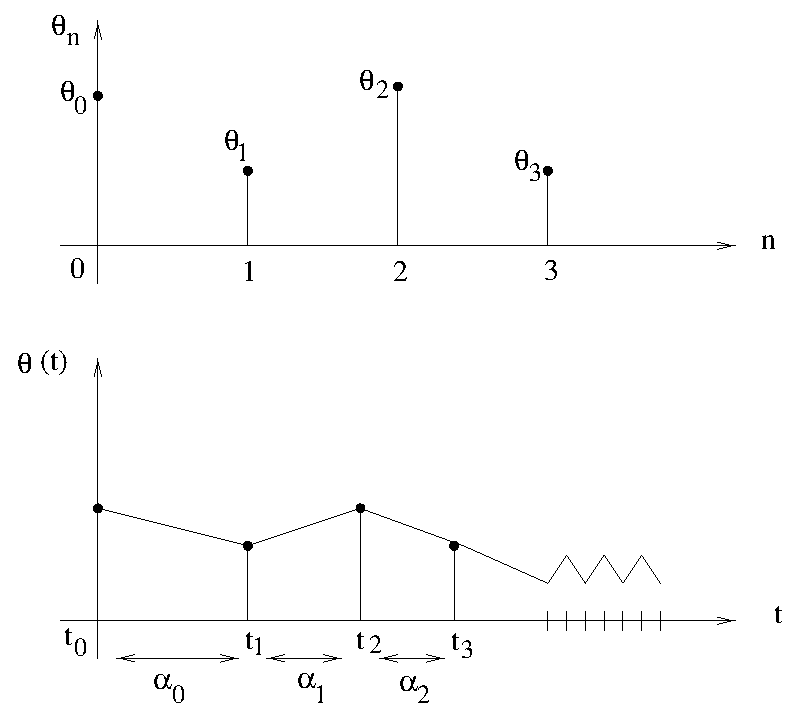
\includegraphics{FIGS/ch6_fig1a.eps}}
\end{center}


Note that over a fixed $\Delta t$, the ``total gain'' is approximately
constant:
$$
\sum_{k\in K(t, \Delta t)} \alpha_k \simeq \Delta t\,,
$$
where $K(t,\Delta t) = \{k: t \le t_k < t+ \Delta t\}$.

Now:
$$
\theta(t+\Delta t) = \theta(t) + \sum_{k\in k(t, \Delta t)} \alpha_k [h(\theta_n)
+\om_n] \,.
$$
\begin{itemize}
\item
For $t$ large, $\alpha_k$ becomes small and the summation is over many
terms; thus the noise term is approximately ``averaged out'':
$\sum \alpha_k \om_k \to 0$.
\item
For $\Delta t$ small, $\theta_k$ is approximately constant over $K(t, \Delta t):
h(\theta_k) \simeq h(\theta(t))$.
\end{itemize}
We thus obtain:
$$
\theta(t+\Delta t) \simeq \theta(t) +\Delta t\cdot h (\theta(t))\,.
$$
For $\Delta t \to 0$, this reduces to the ODE:
$$
\dot \theta(t) = h(\theta(t))\,.
$$

\medskip

To conclude:
\begin{itemize}
\item
As $n\to\infty$, we ``expect'' that the estimates
$\{\theta_n\}$ will follow a trajectory of the ODE $\dot\theta=h(\theta)$
(under the above time normalization).
\item
Note that the stationary point(s) of the ODE are given by
$\theta^*:\;\; h(\theta^*) = 0$.
\item
An obvious requirement for $\theta_n \to \theta^*$ is
$\theta(t) \to \theta^*$
(for any $\theta(0)$).
That is: $\theta^*$ is a {\em globally asymptotically stable} equilibrium of
the ODE.

This may this be viewed as a necessary condition for convergence of
$\theta_n$. It is also sufficient under additional assumptions on
$h$ (continuity, smoothness), and boundedness of $\{\theta_n\}$.
\end{itemize}

% \uu{A Remark on Asynchronous Algorithms}:\quad
% When the stepsize is different for each component of $\theta$, the
% approximating ODE is more involved -- the relative rates should enter
% explicitly.
% Still, there exist specifc results that related
% the above ``synchronous'' ODE to the convergence of the
% asynchronous SA algorithm.


\section{Some Convergence Results}

A typical convergence result for the (synchronous) SA algorithm is the following:

\begin{theorem}\label{thm:SA_1}
Assume G1, N1, and furthermore:
\begin{itemize}
\item[(i)]
$h$ is Lipschitz continuous.
\item[(ii)]
The ODE $\dot\theta=h(\theta)$ has a unique equilibrium point $\theta^*$, which
is globally asymptotically stable.
\item[(iii)]

The sequence $(\theta_n)$ is bounded (with probability 1).
\end{itemize}
Then $\theta_n\to\theta^*$ (w.p.~1), for any initial conditions $\theta_0$.
\end{theorem}


\paragraph{Remarks:}
\begin{itemize}
\item[1.]
More generally, even if the ODE is not globally stable, $\theta_n$ can be shown to converge
to an {\em invariant set} of the ODE (e.g., a limit cycle).
\item[2.]
Corresponding results exist for the asynchronous versions, under suitable
assumptions on the relative gains.
\item[3.]
A major assumption in the last result in the boundedness of $(\theta_n)$.
In general this assumption has to be verified independently. However, there
exist several results that rely on further properties of $h$ to deduce
boundedness, and hence convergence.
\end{itemize}


The following convergence result from B.~\&T.~(1996) relies on
 \uu{contraction} properties of $H$, and applies to the
asynchronous case.
It will directly apply to some of our learning algorithms.
We start with a few definitions.

\begin{itemize}
\item
Let $H(\theta) = h(\theta) + \theta$, so that $h(\theta) = H(\theta) - \theta$.
\item
Recall that $H(\theta)$ is a {\em contraction operator} w.r.t.\ a norm
$\|\cdot\|$ if
$$
\| H(\theta_1) - H(\theta_2)\| \le \alpha \| \theta_1 - \theta_2\|
$$
for some $\alpha < 1$ and all $\theta_1, \theta_2$.
\item
$H(\theta)$ is a {\em pseudo-contraction} if the same holds for a
fixed $\theta_2=\theta^*$.
It easily follows then that $\theta^*$ is a unique fixed point of $H$.
\item
Recall that the {\em max-norm} is given by
$\|\theta\|_\infty = \max_i |\theta(i)|$.
The {\em weighted} max-norm, with a weight vector $w$, $w(i) > 0$, is given by
$$
\|\theta\|_w = \max_i \{ \frac{|\theta(i)|}{w(i)}\}
\,.
$$
\end{itemize}

\begin{theorem}[Prop. 4.4. in B.\&T.]\label{thm:SA_2}
Let
$$
\theta_{n+1}(i) = \theta_n(i) + \alpha_n (i)  [H(\theta_n) - \theta_n +
\om_n]_i\,, \quad i=1, \cdots, d\,.
$$
Assume N1, and:
\begin{itemize}
\item[(a)]
Gain assumption: $\alpha_n(i) \ge 0$, measurable on the ``past'', and satisfy
$$
\sum_n \alpha_n(i) = \infty, \quad \sum_n \alpha_n(i)^2 < \infty \quad
\text{(w.p. 1)}\,.
$$
\item[(b)]
$H$ is a pseudo-contraction w.r.t.\ some weighted max-norm.
\end{itemize}
Then $\theta_n \to \theta^*$ (w.p.\  1), where $\theta^*$ is the unique fixed point
of $H$.
\end{theorem}



\paragraph{Remark on ``Constant Gain'' Algorithms}

As noted before, in practice it is often desirable to keep a non-diminishing
gain.
A typical case is $ \alpha_n(i)\in [\uu\alpha, \oo{\alpha}]$.

Here we can no longer expect ``w.p.\   1'' convergence results.  What can be
expected is a statement of the form:
\begin{itemize}
\item
For $\oo\alpha$ small enough, we have for all $\eps > 0$
$$
\limsupn P (\|\theta_n - \theta^* \| > \eps) \le b(\eps) \cdot
\oo\alpha\,,
$$
with $b(\eps) < \infty$.
\end{itemize}

This is related to ``convergence in probability'', or ``weak convergence''.
We shall not give a detailed account here.

%\section{Gain Selection}
%
%The choice of the gain sequence $(\alpha_n)$ can have drastic effect on the speed of
%convergence. Over the years there have been many suggestions for possible choices,
%which we briefly describe. The discussion is informal,
%under appropriate assumptions on the noise sequence. For more details
%see the book by Spall.
%
%{\em a. Asymptotic Optimality}
%
%Suppose we wish to minimize the asymptotic variance:
%$$ \lim_{\to\infty} E(\theta_n - \theta^*)^2 \.$$
%An optimal choice in this sense is $\alpha_n = \frac{1}{n}$ (pure averaging).
%The asymptotic variance can then be computed using the Central Limit Theorem (CLT).
%
%More precisely, for  $\alpha_n = \frac{a}{n^b}$, $b<2$, we get
%$$
%n^{\frac{b}{2}} (\theta_n -\hat{\theta}) \to_{distr.} N(0,\Sigma) \,,
%$$
%i.e., $\theta_n \sim \theta^* +\frac{1}{n^{\frac{b}{2}} \Sigma$, where
%$\Sigma$ is a fixed matrix (which depends on $a$). \\
%The best rate is obtained for $b=1$. \\
%$\Sigma$ is minimized by the choice of {\em matrix} gains: $a=H(\theta^*)^{-1}$,
%where $H(\theta) = \frac{\partial h(\theta)}(\partial \theta}$ is the Hessian
%matrix.
%
%{\em Averaging} A problem with the above choice is that the function $h$
%(hence the Hessian) are not known in advance. Also the gain sequence may
%decay too fast at the initial stage. An alternative that obtains the
%optimal asymptotic rate is the averaging scheme proposed by
%Polyak and Juditsky (1992):
%
%1. Compute $\theta_n$ with any gain sequence $\alpha_n$ that satisfies the
%usual conditions, and in addition: $\frac{\alpha_{n+1}}{\alpha_n} =1 - o(\alpha_n)$.
%For example, $\alpha_n = \frac{a}{n^b}$ with $0.5<\beta <1$, $a>0$.
%
%2. Take the average:   $\bar{\theta} = \frac{1}{n} \sum_{k=1}^n \theta_k$.
%
%Then $\bar{theta}_n$ has the optimal asymptotic convergence rate.

%{\em b. Heuristics}
%
%The aboce
%
%e slow convergence in the initial phase.
%Once solution is to start with another schedule (see the heuristics below) and then
%revert to $\frac{1}{n}$ for "fine tuning'' in the final stage.
%
%\end{document}

\section{Exercises}

\begin{exercise}[\textbf{Stochastic Approximation}]
Let $\left\{ {{X_n}} \right\}_{n = 0}^\infty $ be an i.i.d. sequence of bounded random variables with mean $\mu $ and variance ${\sigma ^2}$. Consider the following iterative method for estimating $\mu ,{\sigma ^2}$:
\begin{equation*}
    \begin{split}
       {\hat \mu _0} &= {\hat s_0} = 0 ,\\
        {\hat \mu _{n + 1}} &= {\hat \mu _n} + {\alpha _n}\left( {{X_{n + 1}} - {{\hat \mu }_n}} \right) ,\\
        {\hat s_{n + 1}} &= {\hat s_n} + {\alpha _n}\left( {{{\left( {{X_{n + 1}} - {{\hat \mu }_n}} \right)}^2} - {{\hat s}_n}} \right).
     \end{split}
\end{equation*}
Use the ODE method and show that $\left( {{{\hat \mu }_n},{{\hat s}_n}} \right) \to \left( {\mu ,{\sigma ^2}} \right)$ with probability one.
\end{exercise}



\chapter{Basic Convergence Results for RL Algorithms}
%% chapter 7, LCS03, convergence analysis
%\input{header}
%
%% \newcommand{\midarrow}[1]{\stackrel{#1}{\to}}
%
%% \newcommand{\Real}{\mathbb R}
%% \newtheorem{assumption}{Assumption}
%\begin{document}
%
%
%% First page number
%\setcounter{page}{1}
%% PREVIOUS section number
%\setcounter{section}{5}
%% PREVIOUS subsection number
%\setcounter{subsection}{0}
%
%% ***********************************************************************
%\textsc{Reinforcement Learning and Dynamic Programming \hfill Spring 2014$\;$ \\
%Lecture Notes \hfill Shie Mannor and Nahum Shimkin}
%\vspace{-18pt}
%\par
%\hrulefill
%% ***********************************************************************
%
%% {\large
%
%\section{Basic Convergence Results for RL Algorithms}

We establish here some asymptotic convergence results for the basic
RL algorithms, by showing that they reduce to Stochastic Approximation
schemes. We focus on the discounted-cost problem, which is easiest.
Analogous results exist for shortest-path problems under the properness assumption (every policy
terminates in expected finite time).

We do not directly consider here the issue of {\em exploration},
which is essential for convergence to the optimal policy. Thus, where
required we will simply {\em assume} that all actions are sampled
often enough.


\section{Q-learning}

Recall the $Q$-learning algorithm, in the following generalized form:
$$
Q_{n+1} (s,a) = Q_n(s,a) + \alpha_n(s,a)
[r (s,a,s'_{s,a}) + \gamma \max_{{a'}} Q_n (s'_{s,a}, {a'}) - Q_n(s,a)]
$$
where each $s_{s,a}'$ is determined randomly according to
$p(s'|s,a)$.

We allow here $\alpha_n(s,a) = 0$, so that any number of $(s,a)$ pairs can be
updated at each stage.

This iteration can be viewed as an (asynchronous)
Stochastic Approximation algorithm, with $Q\equiv \theta$.
This leads to the following result.

\begin{theorem}[Convergence of $Q$-learning.]
Let $\gamma < 1$, and let  $Q^*$ be the optimal $\gamma$-discounted
$Q$ function. Assume
$$
\sum_{h=0}^\infty \alpha_n (s,a) = \infty, \quad \sum_{n=0}^\infty
\alpha_n(s,a)^2 < \infty \quad
\text{(w.p. 1)} \quad \forall s, a\,.
$$
Then
$$
\lim_{n\to\infty} Q_n(s,a) = Q^* (s,a) \quad \text{(w.p. 1)} \quad \forall s,a \,.
$$
\end{theorem}

\begin{proof}
Define the mapping $H$ over the set of $Q$-functions as follows:
\begin{align*}
(H Q) (s,a) & = \sum_{s'} P(s'|s,a) [r(s, a,s') + \gamma \max_{a'} Q(s',{a'})]\\
& = E[r(s,a,s_{n+1}) + \gamma \max_{a'} Q(s_{n+1},{a'})|s_n=s,a_n=a]\,.
\end{align*}
The above Q-learning algorithm can thus be written in the standard SA form,
with the noise vector $\om_n$ given by:
$$
\om_n(s,a) = r(s,a,s'_{s,a}) + \gamma \max_{a'} Q_n (s'_{s,a}, {a'}) -
(HQ) (s,a)
\,.
$$
We proceed to verify the assumptions in Theorem \ref{thm:SA_2}:
\begin{itemize}
\item[(a)]
Step-size requirements hold here by assumption.
\item[(b)]
Noise Assumption N1:
The definition of $\om_n$ immediately implies that
$ E (\om_n(s,a) | \cF_n) = 0$.
It is further easily seen that
$$
E (\om_n(s,a)^2 | \cF_n) \le \text{ quadratic function of \ }
\|Q\|_{\infty}\,.
$$
\item[(c)]
Contraction:
As with the discounted DP operator, it may be verified that $H$ is a
$\gamma$-contraction w.r.t.\ the max-norm.
\end{itemize}
The required convergence result therefore follows by Theorem \ref{thm:SA_2}.
\end{proof}



\paragraph{Remarks on basic (on-policy) Q-learning:}
\begin{itemize}
\item
In the basic version of the algorithm, we follow a state-action sequence
$(s_n, a_n; n=0,1,\cdots)$ which is generated by some arbitrary policy,
and at time $n$ update $Q(s, a)$ only for $(s,a)=(s_n,a_n)$.
This corresponds to the choice of gains:
$$
\alpha_n(s,a) > 0 \quad \text{iff} \quad
(s,a) = (s_n, a_n)
\,.
$$
\item
For $(s,a)= (s_n, a_n)$, a typical choice for $\alpha_n$ is
$$
\alpha_n(s,a) = \hat\alpha(N_n (s,a))
$$
where $N_n$ is the number of previous visits to $(s,a)$, and
$\hat\alpha(k)$ satisfies the standard assumptions.
\item
For the step-size requirements in the theorem to hold in this case it is
required that each $(s,a)$ pair is visited ``relatively often''.
This should be verified by appropriate exploration policies!
\end{itemize}

\paragraph{Undiscounted case:}
Under appropriate ``Stochastic Shortest Path''
assumptions, it can be shown that $H$ is a pseudo-contraction w.r.t.\ some
weighted max-norm.
Convergence follows as above.


\section{Convergence of TD($\la$)}

TD(0) can be analyzed exactly as Q-learning learning.
TD($\la$) is slightly more involved.
Recall the ``on-line" version of TD($\la$):
$$
V_{n+1}(s)=V_n(s)+\alpha_n e_n(s)d_n\,,\quad s\in S
$$
where
\begin{align*}
\alpha_n & = \mbox{\rm gain} \\
e_n(s) & = \mbox{\rm eligibility trace coefficient}\\
d_n & = r_n + \gamma V_n(s_{n+1})-V_n(s_n)\\
\gamma& = \mbox{\rm discount factor}
\end{align*}

\paragraph{Requirements on the Eligibility Trace:}

Several variants of the algorithm are obtained by different choices
of $e_n(s)$, such as:
\begin{itemize}
\item[(a)] First-visit TD($\la$):
$$
e_n(s)=(\gamma\la)^{n-m_1(s)} 1\{n\ge m_1(s)\} \,,
$$
$m_1(s)$ is the time of first visit to state $s$ (during the present run).
\item[(b)] Every-visit TD($\la$):
$$
e_n(s)=\sum_{j:m_j(s)\le n}   (\gamma\la)^{n-m_j(s)} \,,
$$
$m_j(s)$ is the time of $j^{th}$ visit to state $s$.
\item[(c)]  First-visit with stopping:
$$
e_n(s)=(\gamma\la)^{n-m_1(s)} 1\{m_1(s)\le n \le \tau\}
$$
where $\tau$ is some stopping time -- e.g., end of simulation run, or arrival
to a state whose value $V(s)$ is known with high precision. $e_n(s)$ is
restarted after $\tau$.
\end{itemize}



A {\em general set of requirements} on the eligibility coefficients $e_n(s)$, which
includes the above cases, is given as follows:
\begin{itemize}
\item[(a)]
$e_0(s)= 0$, $e_n(s)\ge 0$.
\item[(b)]
$e_n(s)\le \gamma e_{n-1}(s)$ if $s_n\not= s$, \\
$1\le e_n(s)\le 1+ \gamma e_{n-1}(s)$ if $s_n= s$.
\item[(c)]
$e_n(s)$ is measurable on the past.
\end{itemize}

\paragraph{Convergence:}

We now argue as follows.
\begin{itemize}
\item
It may be seen that TD($\la$) is in the form of the Stochastic
Approximation algorithm, with $\theta_n\equiv V_n$, and
$$
h(\theta)\equiv h(V) = (h(V)(s),\,s\in S)\,,
$$
\begin{eqnarray*}
h(V)(x) &=& E^\pi [d_n|V_n=V,\, s_n=s]\\
&=& \sum_a \pi(a|s)[r(s,a)+\gamma\sum_{s'} p(s'|s,a)V(s')]-V(s) \\
&:=& (HV)(s) -V(s) \,.
\end{eqnarray*}
Here $\pi$ is the {\em fixed stationary} policy that is used.
\item
For $0<\gamma<1$ it is obvious that $H$ is a contraction operator.
\item
For convergence we now need to verify  that the effective  gains
$\alpha_ne_n(s)$ satisfy the ``usual assumptions". This may be
verified by requiring that each state is visited ``relatively often".
\end{itemize}

For $\gamma=1$, a similar argument may be made for SSP (Stochastic Shortest Path)
problems.


%
% \subsection{An ODE Perspective}
%
% It is instructive to examine the convergence of these algorithms via the
% ODE approach.
%
% Recall that Q-learning is in the form of the SA algorithm,
% with $h(Q)=H(Q)-Q$, and $H$ is a max-norm contraction.
%
% The corresponding ODE is
% $$
% \dot Q = H(Q)-Q
% $$
% It can be shown that if $H$ is a max-norm contraction, then the fixed
% point $Q^*$ of $H(Q)=Q$ is globally asymptotically stable.
%
% To establish convergence it only remains to show that $\{\hat{Q}_n\}$
% is a bounded sequence (w.p.\  1). This is usually done via separate
% analysis. However, a recent result
% shows that boundedness too can be deduced via the ODE approach
% (Borkar and Meyn, 2000):
%
% Given $h(Q)\equiv h(\theta)$, define
% $$
% h_{\rho}(\theta)\dfn h(\rho\theta)/\rho\,,
% $$
% and assume that $h_\infty(\theta)\dfn\lim_{\rho\to\infty}h_{\rho}(\theta)$
% exists.
%
% This limit would exist when $h$ has some  ``linear nature". For example,
% for Q-learning we have that $h_{\infty}(Q)\; =$ same as $h(Q)$, but
% with 0 rewards, $r(s,a)\equiv 0$.
%
% {\bf Theorem:} In the basic SA algorithm, if $h_{\infty}$ is well defined, and
% the normalized ODE
% $$
% \dot \theta = h_{\infty}(\theta)
% $$
% has $\theta^*=0$ as an asymptotically stable equilibrium point, then
% $\sup_n |\theta_n| < \infty$ (w.p.  1).
%
% A similar conclusion holds for the ``distributed" versions under appropriate
% conditions.



\section{Actor-Critic Algorithms}

Convergence of actor-critic type algorithms is harder to analyze. We describe here some results from
Konda and Borkar (2000).

Recall that the idea is to use a ``fast" estimation loop to obtain $\hat V(s)$,
and a slower loop to update
the policy $\hat \pi$ given $\hat V$.

Let $V_n(s)$ and $\pi_n=(\pi_n(a|s))$ be the estimated value and policy at step
$n$.

\paragraph{Algorithm 1}
\begin{itemize}
\item[a.]
Value-function estimation (generalized TD(0)):
$$
V_{n+1}=V_n(s)+\beta_n(s)[r(s,a_n(s))+\gamma V_n(s_{n+1}(s))-V_n(s)]\,,\quad s\in Y_n
$$
where
\begin{align*}
&  Y_n   \mbox{ \rm -- set of states updated at step $n$} \\
&  \beta_n(s)  \mbox{ \rm -- gains }\\
& s_{n+1}(s)  \mbox { \rm -- next state, chosen with distribution\ }
         \mbox{\rm $p(s') = \sum_a p(s'|s,a)\pi_n(a|s)$.
}
\end{align*}

\item[b.] Policy update:
$$
\pi_{n+1}(a|s)=\pi_{n}(a|s) + \alpha_n(s,a) (( \hat{Q}_n(s,a) - \hat{Q}_n(s,a_0) ))\,,
\quad (s,a) \in Z_n
$$
where
\begin{align*}
& Z_n  \mbox{ \rm -- set of state-action pairs  updated at step $n$} \\
& \alpha_n(s,a) \mbox{ \rm -- gains} \\
& \hat{Q}_n(s,a):=r(s,a)+\gamma V_n(s_{n+1}(s,a))\\
& s_{n+1}(s,a) \mbox{ \rm -- next state, chosen according to $p(s'|s,a)$} \\
& a_0 \mbox { \rm -- a fixed reference action (for each state).}
\end{align*}

\item[b'.] Policy normalization:

For each $s$, project the vector $(\pi_{n+1}(a|s),\; a\not= a_0)$ unto the
following set
of sub-probability vectors:
$$
\{\pi: \pi(a)\ge 0,\;\; \sum_{a\not = a_0}\pi(a)\le 1\}
$$
and then let $\pi_{n+1}(a_0|s)=1-\sum_{ a\not = a_0}\pi_{n+1}(a|s) $.

% The above scheme can be considered a ``variable structure" automaton". Note that
% the range of $Q$ is not known in advance.

\item[c.] Rate requirements:

We first require that all updates are executed relatively often, namely that for
some $\Delta>0$,
$$
\liminf_{n\to\infty}\frac{n_1(s)}{n} \ge \Delta\,,\quad
\liminf_{n\to\infty}\frac{n_2(s,a)}{n} \ge \Delta\,,
$$
where
\begin{align*}
n_1(s) &= \sum_{k=1}^n 1\{s\in Y_k\} \\
n_2(s,a) &= \sum_{k=1}^n 1\{(s,a) \in Z_k\} \,.
\end{align*}

The gains are determined by some sequences $\alpha(m)$ and $\beta(m)$, as
$$
\alpha_n(s,a)=\alpha(n_2(s,a))\,,\quad \beta_n(s)=\beta(n_1(s)) \,.
$$
The sequences $\alpha(m)$, $\beta(m)$  should satisfy:

(1) The standard summability assumptions.

(2) Policy updates are ``slower":  $\lim_{m\to\infty}\frac{\alpha(m)}{\beta(m)}=0$.

(3) Some additional technical assumptions ...

All these requirements are satisfied, e.g., by
$\alpha(m)=\frac{1}{m\log m}$, $\beta(m)=\frac{1}{m}$.
\end{itemize}

Under these assumptions, Algorithm 1 converges to the optimal value and
policy.



\paragraph{Algorithm 2:}

Same as Algorithm 1, except for the policy update (b):
$$
\pi_{n+1}(a|s)=\pi_n(a|s)+a_n(s,a)[\{\hat Q_n(s,a)-V_n(s)\}\pi_n(a|s)+\xi_n(s,a)
] \,.
$$
$\xi_n(s,a)$ are sequences of  ``small" noise terms, these are needed to prevent
 the algorithm
from getting stuck in the wrong ``corners".


\paragraph{Algorithm 3:}

Same as Algorithm 1, except for  (b):
$$
w_{n+1}(a|s)=w_n(a|s)+\alpha_n(s,a)[\hat Q_n(s,a)-V_n(s)]
$$
and
$$
\pi_n(s,a):=\frac{\exp(w_n(s,a))}{\sum_{a'}\exp(w_n(s,a'))} \,.
$$


% Remark:  Compare these algorithms to the Static Reinforcement Learning chapter.

In all these variants, convergence is proved using a ``two-time scale"
Stochastic Approximation framework, the analysis is based on the ODE
method which couples a ``fast"
ODE (for $V$) and a ``slow" ODE  (for $\pi$).

%
%% }
%% large ended
%
%\end{document}
%~


\chapter{Approximate Dynamic Programming}
%% chapter 7, LCS03, convergence analysis
%\input{header}
%\usepackage{verbatim}
%\usepackage[latin1]{inputenc}
%\usepackage{tikz}
\usetikzlibrary{calc}
\usetikzlibrary{shapes,arrows}
%\usepackage{enumerate}
%% \newcommand{\midarrow}[1]{\stackrel{#1}{\to}}
%
%% \newcommand{\Real}{\mathbb R}
%% \newtheorem{assumption}{Assumption}
%\begin{document}
%
%
%% First page number
%\setcounter{page}{1}
%% PREVIOUS section number
%\setcounter{section}{6}
%% PREVIOUS subsection number
%\setcounter{subsection}{0}
%
%% ***********************************************************************
%\textsc{Reinforcement Learning and Dynamic Programming \hfill Spring 2014$\;$ \\
%Lecture Notes \hfill Shie Mannor and Nahum Shimkin \\
%\hfill Scribed by Michal Zarrouk}
%\vspace{-18pt}
%\par
%\hrulefill
%% ***********************************************************************
%
%% {\large
%
%
%\section{Approximate Dynamic Programming}
Recall Bellman's dynamic programming equation
$$V(s) = \max_{a \in A} \left\{R(s,a) + \gamma \sum_{s' \in S} p(s'|s,a)V(s')\right\},$$
or in operator form, $\underline{V}=T\underline{V}$, where $T$ is the Bellman operator.

Dynamic programming requires knowing the model and is only feasible for small problems.
In large scale problems, we face the \textbf{3 curses of dimensionality}:

\begin{enumerate}\negspace
\item $S$ may be large, such that even writing down the policy is difficult. Moreover, $S$ may be continuous, for example in robotics applications.
\item $A$ may be large. Example: resource allocation, where we have several projects and need to assign different resources to each project.
% Note: give details
\item $p(s'|s,a)$ may be complicated: computing $p(s'|s,a)$ requires summing over many random events. Example: resource allocation.
\end{enumerate}

\section{Approximation approaches}
There are 4 approaches to handle the curses of dimensionality:
\begin{enumerate}\negspace
\item \textbf{Myopic}: When $p(s'|s,a)$ is approximately uniform across $a$, we may ignore the state transition dynamics and simply use $a^\pi(s)\approx \underset{a \in A}{\operatorname{argmax}} \{R(s,a)\}$. If $R(s,a)$ is not known exactly -- replace it with an estimate.

\item \textbf{Lookahead policies}: Rolling horizon/model-predictive control.\\
Simulate a horizon of $T$ steps, and use
$$a^\pi(s_t|\theta) = \underset{\pi' \in \Pi}{\operatorname{argmax}}\  \mathbb{E} \left[\sum_{t'=t}^{t+T} R(s_{t'},y^{\pi'}(s_{t'}))\right]$$

\item \textbf{Policy function approximation}\\
Assume policy is of some parametric function form $\pi = \pi(\theta), \ \ \theta \in \Theta$, and optimize over function parameters.\\
\begin{example}[Inventory management]
Consider an inventory management problem, in which the state is the inventory level $s_t$, the demand is $d_t$ and the action is the replenishment level $a_t$. The dynamics are given by:
$$s_{t+1} = [s_t + a_t-d_t]^+.$$
The immediate reward is:
$$R_t = R \min\{d_t,s_t+a_t\} - c_a a_t -C[s_t + a_t-d_t]^+,$$
where $R$ is the profit in satisfying the demand, $c_a$ is the ordering cost, and $C$ is the cost of not satisfying a demand.

One possible replenishment policy is:
$$a^\pi(s_t|\theta) = \begin{cases} 0 & s_t > q\\Q-s_t & s_t \le q \end{cases}, \ \ \ \theta=(q,Q).$$
A different possibility is the \emph{softmax} policy, given by
$$p(s,a) = \frac{e^{-\theta\alpha(s,a)}}{\sum_{a'} e^{-\theta\alpha(s,a')}}, \ \ \mathrm{where}\ \ \alpha=R(s,a)\ \ \mathrm{or} \ \ \alpha=Q(s,a).$$
\end{example}

\item \textbf{Value function approximation}\\
Assume $V(s)\approx f(s,\theta)$ where $f$ is some approximation function, and optimize over the parameters $\theta$.\\
The most standard model is a linear combination of some $k$ features (which are not necessarily linear):
$$\bar{V}(s|\theta) = \sum_{j=1}^k \theta_j \phi_j(s),$$
where $\theta_j$ are the model parameters and $\phi_j$ are the model's \emph{features} (a.k.a. basis functions).\\
Given $\bar{V}$, we can derive a policy by choosing the \emph{greedy} action with respect to $\bar{V}$ (corresponding to a lookahead of 1 time step). If a model or a simulator is also available, we can also use a longer lookahead.\\
\\
Example: a chess game with $K$-step lookahead\\
\tikzstyle{block} = [rectangle, draw,
    text width=7em, text centered, rounded corners, minimum height=4em]
\tikzstyle{blocks} = [rectangle, draw,
    text width=4em, text centered, rounded corners, minimum height=4em]
\tikzstyle{lblock} = [rectangle, draw,
    text width=17em, text centered, rounded corners, minimum height=4em]
\tikzstyle{line} = [draw, -latex']
\begin{tikzpicture}[node distance = 1cm, auto]
    % Place nodes
%    \node [blocks] (a) {Chess game model};
    \node [block] (b) {Feature extraction\\$\phi_1(s),...,\phi_k(s)$};
    \node [block, right of = b, node distance=1.3in] (c) {Compute value\\function weights\\$\theta_1,...,\theta_k$};
    \node [block, right of = c, node distance=1.3in] (d) {$\bar{V}(s)=f(s,\theta)$};
    \node [lblock, right of = d, node distance=2.1in] (e) {\small$\pi(s_t) = \underset{\pi' \in \Pi}{\operatorname{argmax}}\  \mathbb{E}^{\pi'} \left[\sum_{t'=t}^{t+K-1} R(s_{t'}) + \bar{V}(s_{t+K}))\right]$};
    % Draw edges
%    \path [line] (a) -- (b);
    \path [line] (b) -- (c);
    \path [line] (c) -- (d);
    \path [line] (d) -- (e);
\end{tikzpicture}

\paragraph{Issues:}
\begin{enumerate}
\item Choosing the parametric class $\phi$ (architecture): e.g., Radial Basis Functions (RBFs) or kernels. The difficulty is that the value function structure may be hard to know in advance.
\item Tuning the weights $\theta$ (learning): here we focus on simulation.\\
In the linear architecture, we can write
$$\tilde{V}(s;\theta)=\phi(s)^\top \theta$$
(replacing $\theta$ with $r$ for the parameters), or in matrix-vector form,
$$\tilde{ {V}}( {\theta}) =  { {\Phi}} { \theta}$$
Therefore tuning the parameters $ {\theta}$ reduces to approximating $ {V} \in \mathbb{R}^{|S|}$ on $\mathcal{S}=\{  { {\Phi}} {\theta}:  {\theta} \in \mathbb{R}^k\} \subseteq  \mathbb{R}^{|S|} $.

\end{enumerate}

\end{enumerate}

\section{Lookahead Policies}

We will discuss several variants of lookahead policies. We focus on systems with a discrete, and `small enough' action space, but a large, possibly infinite state space.

The main idea in lookahead policies is that when we are at some state $s$, we will only search `around' the state $s$ for the next action $\pi(s)$. After we play the action, we observe the next state, and repeat the search.
Thus, we do not need to consider the whole state space in advance, but only consider regions in state space which we actually visit.
In the control literature, this idea is often called Model Predictive Control (MPC).

\subsection{Deterministic Systems: Tree Search}
The simplest example of a lookahead policy is tree search in a deterministic system.

Given $s$, and a (deterministic) simulator of the system, we can simulate the next state for every possible action, building a tree of possible trajectories of the system, starting from $s$, and continuing to some depth $k$. 
We then choose an action by:
$$\pi(s) = \underset{\pi' \in \Pi}{\operatorname{argmax}}\  \left[\left.\sum_{t=0}^{k} \gamma^t r(s_{t},{\pi'}(s_{t})) \right| s_0 = s\right],$$
Which can be solved using dynamic programming.

In this approach, the computation in each step requires $O(|A|^{k})$ calls to the simulator for building the tree, and $O(k|A|^{k})$ computations for searching the tree. Note that \emph{there is no dependence on $|S|$}. The depth $k$ should be chosen `deep enough' to results in meaningful actions. For example, in a discounted setting, recall that the $k$-horizon value function satisfies 
$\|V^k(s)-V^*(s)\|_\infty \leq \gamma^k\left( \frac{R_{max}}{1-\gamma}\right),$ which can be used to set $k$.

\subsection{Stochastic Systems: Sparse Sampling}
When the system is stochastic, we cannot simply build a tree of possible future trajectories. If we sample next states from our simulator, we can build a \emph{sampled} version of a search tree. Here, for each state $s$ and action $a$ in the tree, we will sample $C$ next states $s'_1,\dots,s'_C$. Then, the backup at $s,a$ will be $Q(s,a) = \frac{1}{C}\sum_{i=1}^C r(s,a) + \gamma \max_{a'} Q(s'_i,a')$.
That is, we replaced the expectation in the Bellman update with an empirical average. Since the average concentrates around the mean (e.g., by Hoeffding inequality), it is expected that the empirical averages will closely represent their expectations.

The following result is shown in \cite{kearns2002sparse}. The constants $k$ and $C$ can be set such that with a per-state running time of $(\frac{|A|}{\epsilon (1-\gamma)})^{O\left(\frac{1}{1-\gamma}\log \frac{1}{\epsilon (1-\gamma)}\right)}$, the obtained policy is $\epsilon-$optimal, i.e., $\|V^k(s)-V^*(s)\|_\infty \leq \epsilon$. Note again that there is no dependence on $|S|$.

\subsection{Monte Carlo Tree Search}
While the sparse sampling above does not depend on $|S|$, the exponential dependence on the horizon and number of actions makes it impractical for many cases. The insight in Monte-Carlo Tree Search (MCTS) is that investing the same simulation efforts for all possible future actions is wasteful, and we should instead focus our search efforts on the \emph{most promising} future outcomes.

The first idea in MCTS is to replace the stage-wise tree building approach with a rollout-based approach, as shown in Figure \ref{fig:mcts}. Here, we roll out complete trajectories of depth $k$, and build the tree progressively from these rollouts. The method \textbf{Evaluate(state)} is used to evaluate the last state in the rollout. This could be the reward of the state, or an estimated value function (as in the chess example above). Another approach, which has become common in games such as Go and Chess, is to simulate a game starting from state $s$ with a predetermined policy, until termination, and evaluate the state by the empirical return along the simulation trajectory.
The method \textbf{UpdateValue} is used to build the tree. It maintains both the sum of returns from a state action pair $Q_{sum}(s,a)$ (summing over all trajectories that visited this state), and the number of visits to the state and state-action pair, $N_s$ and $N_{sa}$. The value of a state-action pair is the average $\frac{Q_{sum}(s,a)}{N_{sa}}$. To understand why this approach could be beneficial, consider a state that is visited multiple times. Thus, after several visits, we have some information about which actions are more promising, and could use that to bias the rollout policy to focus on promising trajectories. We need to make sure, however, that we also \emph{explore} often enough, so that we do not miss important actions by incorrect $Q$ estimates in the beginning.
The key to an efficient MCTS algorithm, therefore, is in the \textbf{selectAction} method, which should balance exploration and exploitation.

\begin{figure}[h]
    \centering
    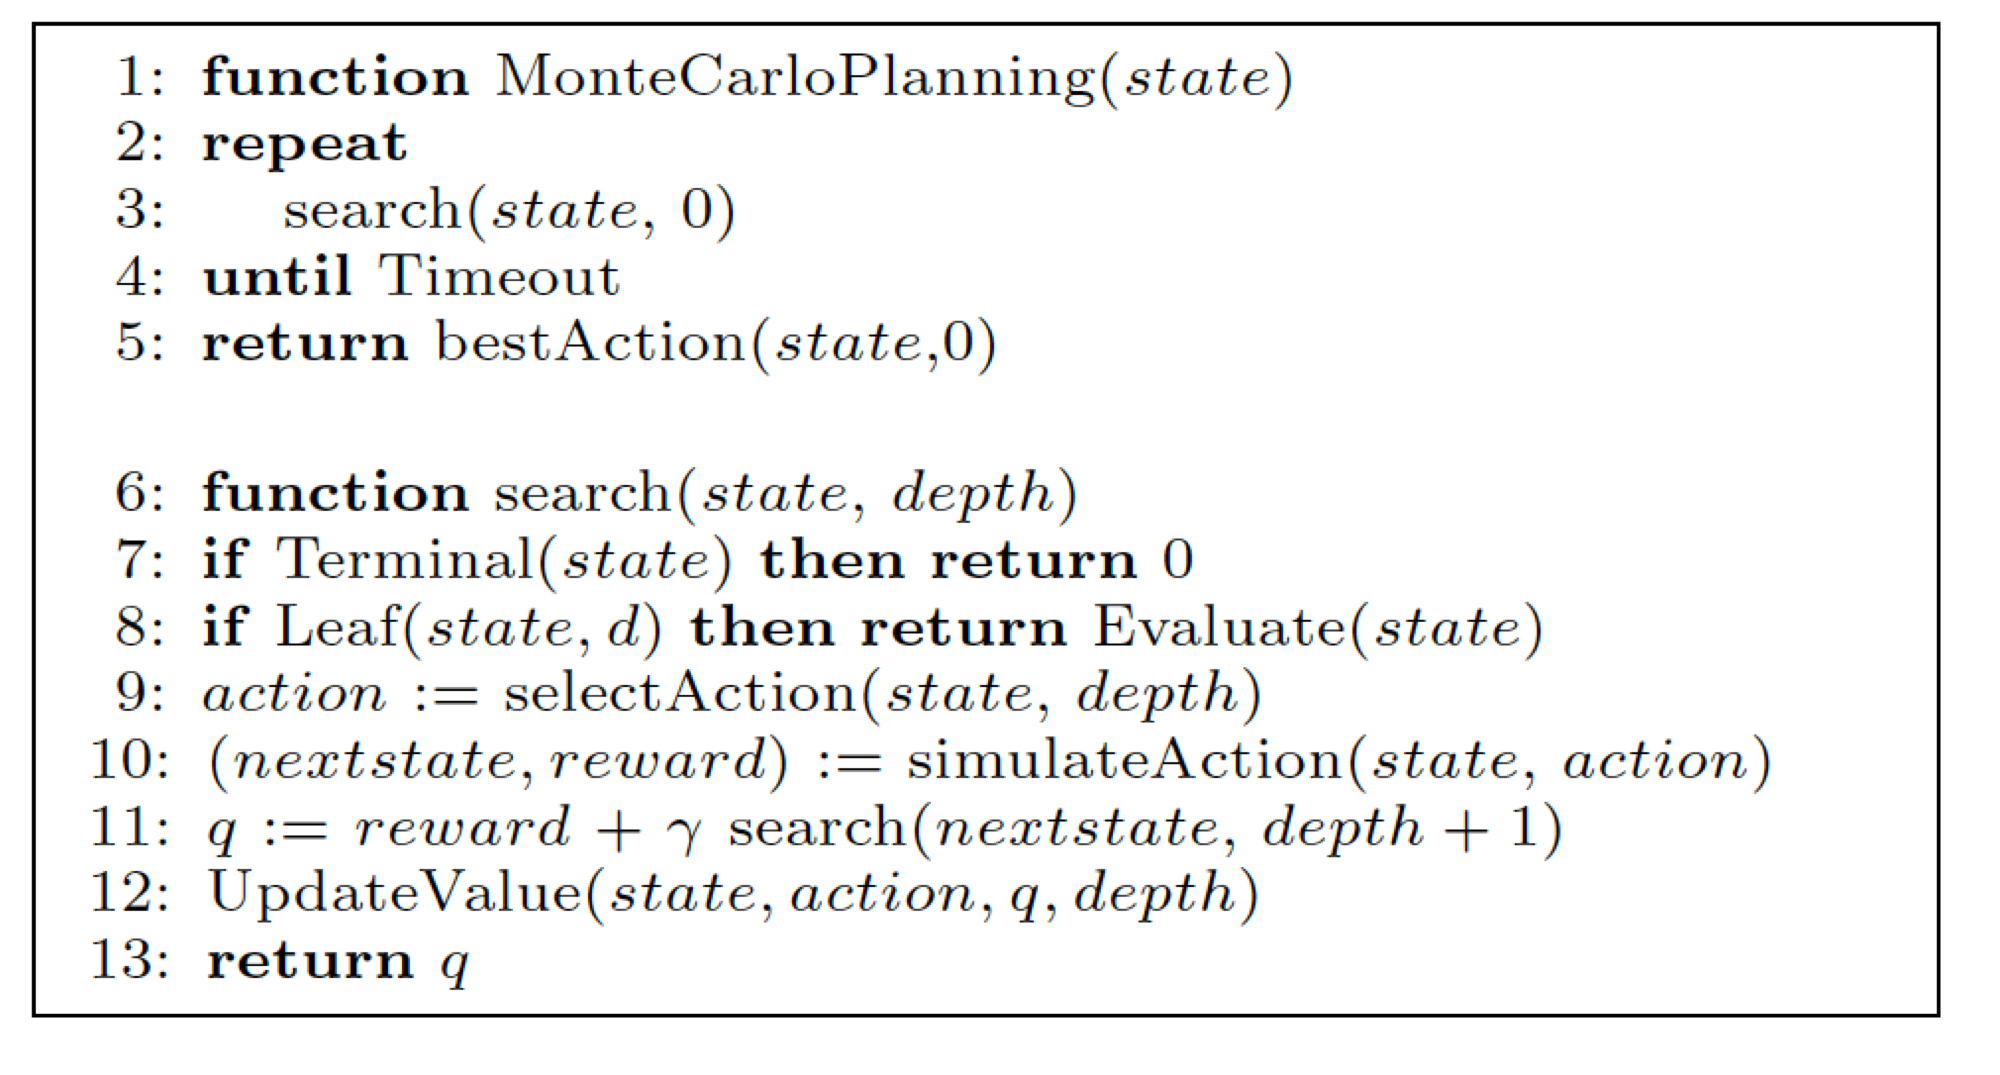
\includegraphics[width=0.8\textwidth]{FIGS/uct.png}
    \caption{Generic Monte-Carlo Planning Algorithm (from\cite{kocsis2006bandit})}
    \label{fig:mcts}
\end{figure}

The UCT algorithm of Kocsis and Szepesv´ari~\cite{kocsis2006bandit} selects actions that maximize $Q(s,a) + UCT(s,a)$, where the \emph{upper confidence bound} is given by: 
$$
UCT(s,a) = C \sqrt{\frac{\log N_s}{N_{sa}}},
$$
where $C$ is some constant. Intuitively, $UCT$ prefers actions that are either promising (high $Q$) or under-explored (low $N_{sa}$). Later in the course we will show that this specific formulation is actually optimal in some sense.

In many practical problems, UCT has been shown to be much more efficient than tree-building methods. MCTS based on UCT is also the most prominent method for solving games with high branching factors such as Go. 

\section{Approximation methods in value space}
\begin{enumerate}\negspace
\item Approximate policy iteration: approximate $V^\mu$; improve $\mu$; repeat.
\item Approximate value iteration / Q-learning: $\hat{Q}(s,a)\approx {\phi}(s,a)^\top {\theta}$
% \item Bellman error minimization:
% $$ \min_\theta \  \mathbb{E}_s \left[\left(\tilde{V}(s;\theta)-T\tilde{V}(s;\theta)\right)^2\right]$$
% where $T$ is the Bellman operator and $\mathbb{E}_s$ is w.r.t. some distribution over the states.
\item Linear programming: not discussed.
\end{enumerate}

Note that both $V$ and $Q$ are mappings from a state (or state-action) to $\mathbb{R}$. When the state space is large, we will not be able to calculate the value for every state, but instead, fit some function to a few states values that we will calculate. This is similar to a \emph{regression} problem, which our development will be based on, but as we will see, we will also need to account for the dynamic nature of the problem to develop approximate optimization algorithms.

\subsection{Approximate Policy Evaluation}

We start with the simplest setting - approximating the value of a fixed policy. A direct approach for this task is through regression, which we will now review. 

\subsubsection{Least Squares Regression}
Assume we have some function $y = f(x)$, and a distribution over a finite set of inputs $\xi(x)$. 
We want to fit a parametric function $g(x;\theta)$ to our data such that $g$ approximates $f$. The least squares approach solves the following problem:
$$
\min_\theta \mathbb{E}_{x\sim\xi} (g(x;\theta) - f(x))^2.
$$
When $g$ is linear in some features $\phi(x)$, i.e., $g(x;\theta) = \theta^T \phi(x)$, then we can write the above equation in vector notation as
$$
\min_\theta (\Phi \theta - Y)^T \Xi (\Phi \theta - Y),
$$
where $Y$ is a vector of $f(x)$ for every $x$, and $\Phi$ is a matrix with $\phi(x)$ as its rows. The solution is given by:
$$
\theta_{LS} = (\Phi^T \Xi \Phi)^{-1} \Phi^T \Xi Y.
$$
Note that $\Phi \theta_{LS}$ denotes the approximated function $g(x;\theta)$. We will call this the \emph{projection} of $y$ onto the space spanned by $\theta^T \phi(x)$, and we can write the projection operator explicitly as:
$$
\Pi_\epsilon Y = \Phi \theta_{LS}(Y) = \Phi (\Phi^T \Xi \Phi)^{-1} \Phi^T \Xi Y.
$$

In the non-linear case, a common approach is to solve the least squares problem by gradient descent, i.e., $\theta_{k+1} = \theta_k - \alpha_k \nabla_\theta \mathbb{E}_{x\sim\xi} (g(x;\theta) - f(x))^2,$ where the gradient is simply $2 \mathbb{E}_{x\sim\xi} (g(x;\theta) - f(x))\nabla_\theta g(x;\theta)$. 

In a practical case, we are given $N$ data samples $\{ x_i, y_i \}: x_i\sim \xi, y_i=f(x_i)$. The least squares solution can be approximated from the samples as:
$$
\min_\theta \sum_i (g(x_i;\theta) - y_i)^2,
$$
The stochastic gradient descent (SGD) version of this update is
$$
\theta_{k+1} = \theta_k - \alpha_k (g(x_i;\theta_k) - y_i)\nabla_\theta g(x_i;\theta_k).
$$

For the linear case, we can solve directly:
$$
\hat{\theta}_{LS} = (\hat{\Phi}^T \hat{\Phi})^{-1} \hat{\Phi}^T \hat{Y},
$$
where in this case the rows of $\hat{\Phi}$ and $\hat{Y}$ are given by the $N$ samples. By the law of large numbers, we have that $\frac{1}{N}(\hat{\Phi}^T \hat{\Phi}) \to (\Phi^T \Xi \Phi)$ and $\frac{1}{N}\hat{\Phi}^T \hat{Y} \to \Phi^T \Xi Y$, thus the sampled solution converges to the solution $\theta_{LS}$ above.

\subsubsection{Approximate Policy Evaluation: Regression}

The direct approach to policy evaluation: Evaluate $V^\mu(s)$ only for several states (e.g. by simulation) and interpolate, e.g., using least squares regression: $\Phi \theta = \Pi V^\mu$. This method is simple, however, it has several drawbacks. The first is that value estimates typically have a large variance, as they accumulate rewards from multiple states in the future. The second is that we need to wait for full simulations to complete before updating the value estimate. Practically, this can take too long in some problems. 

We next describe an alternative approach, using the fact that the value function satisfies Bellman's equation.

\subsubsection{Approximate Policy Evaluation: the Projected Bellman Equation}

% A key step in approximate policy iteration here is the policy evaluation: given $\mu$ we would like to approximate $V^\mu$. There are two main methods for approximate policy evaluation:
% \begin{enumerate}
% \item Direct approach: Evaluate $V^\mu(s)$ only for several states (e.g. by simulation) and interpolate, e.g., using least squares regression: $\Phi \theta = \Pi V^\mu$. This method is simple, however, it has several drawbacks. The first is that value estimates typically have a large variance, as they accumulate rewards from multiple states in the future. The second is that we need to wait for full simulations to complete before updating the value estimate. Practically, this can take too long in some problems. 
% \item 
The indirect approach to policy evaluation is based on the projected Bellman equation (PBE). Recall that $V^\mu(s)$ satisfies the Bellman equation: $V^\mu = T^\mu V^\mu$. We can evaluate $V^\mu(s)$ by projecting the Bellman operator $T^\mu$ onto $\mathcal{S}$ (the subspace spanned by $\Phi$):
\begin{equation*}
    \Phi \theta = \Pi T^\mu \{\Phi \theta\},
\end{equation*}
where $\Pi$ is the projection operator onto $\mathcal{S}$ under some norm.
    % \begin{equation*}
    %     \theta_k= \underset{\theta}{\operatorname{argmin}} \{||\Phi \theta - T^{\mu_k}\Phi \theta_k||_\epsilon^2\}.
    % \end{equation*}
Includes:
\begin{itemize}
\item Temporal differences - TD(0): online solution of the PBE.
% $\Phi \theta = \Pi T^\mu \{\Phi \theta\}$, where $\Pi$ is the projection operator onto $\mathcal{S}$ under some norm.\\
\item Least-squares policy evaluation - LSPE(0): simulation-based form
\begin{align*}\Phi \theta_{k+1} = \Pi T^\mu \{\Phi \theta_k\} + \mathrm{noise}.\end{align*} 
\item Least-squares temporal differences - LSTD(0): batch solution of the PBE.
\end{itemize}
% \end{enumerate}

We now discuss the indirect approach to policy evaluation.
\\
Define the weighted Euclidean inner product:
$$\langle V_1,V_2\rangle_\epsilon = \sqrt{\sum_{i=1}^n \epsilon_i V_1(i)V_2(i)}, \ \ \epsilon_i\ge0,$$
and the induced weighted Euclidean norm:
$$||V||_\epsilon = \sqrt{\sum_{i=1}^n \epsilon_i V(i)^2}, \ \ \epsilon_i\ge0,$$
and let $\Pi_\epsilon$ be the operator of projection onto $\mathcal{S}$ w.r.t. this norm:
\begin{align*}\Pi_\epsilon V &=\underset{V' \in \mathcal{S}}{\operatorname{argmin}} \ ||V'-V||_\epsilon =\\
&= \Phi \theta \ \ \ \mathrm{s.t.} \ \ \theta = \underset{\theta' \in \mathbb{R}^k}{\operatorname{argmin}} \ ||\Phi \theta' - V||_\epsilon.\end{align*}

We want to solve the projected Bellman equation (PBE):
\begin{equation}\label{eq:PBE}
\Phi \theta^*  = \Pi_\epsilon T^\mu \Phi \theta^*.
\end{equation}
The main reason to consider the approximation in \eqref{eq:PBE} is that, as we shall see, it will allow us to derive efficient sampling based algorithms with provable error guarantees.

\subsection{Existence, Uniqueness and Error Bound on PBE Solution}
We are interested in the following questions:
\begin{enumerate}
\item Does the PBE \eqref{eq:PBE} have a solution?
\item When is $\Pi_\epsilon T^\mu$ a contraction, and what is its fixed point?
\item If $\Pi_\epsilon T^\mu$ has a fixed point $\theta^*$, how far is it from $\Pi_\epsilon V^\mu$?
\end{enumerate}
Let us assume the following:
\begin{assumption}\label{ass:recurrent}The Markov chain corresponding to $\mu$ has a single recurrent class and no transient states. We further let
$$\epsilon_j = \lim_{N\rightarrow \infty} \frac{1}{N} \sum_{t=1}^N p(s_t=j|s_0=s)>0,$$
which is the probability of being in state $j$ when the process reaches its steady state, given $s_0=s$.
\end{assumption}
We have the following result:
\begin{proposition}\label{prop:PBE_contraction} Under Assumption \ref{ass:recurrent} we have that
\begin{enumerate}
\item $\Pi_\epsilon T^\mu$ is a contraction operator with modulus $\gamma$ w.r.t. $||\cdot||_\epsilon$.
\item The unique fixed point $\Phi \theta^*$ of $\Pi_\epsilon T^\mu$ satisfies
$$||V^\mu - \Phi \theta^*||_\epsilon^2 \le \frac{1}{1-\gamma^2}||V^\mu-\Pi_\epsilon V^\mu||_\epsilon^2.$$
\end{enumerate}
\end{proposition}
\begin{proof}
We begin by showing the contraction property. We use the following lemma:
\begin{lemma}\label{lem:P_non_expansion} If $P^\mu$ is the transition matrix induced by $\mu$, then
$$\forall z \ \ ||P^\mu z||_\epsilon \le ||z||_\epsilon.$$
\end{lemma}
\begin{proof}
Proof: Let $p_{ij}$ be the components of $P^\mu$. For all $z \in \mathbb{R}^n$:
$$||P^\mu z||_\epsilon^2 = \sum_i \epsilon_i\left(\sum_j p_{ij}z_j\right)^2 \underbrace{\leq}_{\textrm{Jensen}} \sum_i \epsilon_i \sum_j p_{ij} z_j^2 =  \sum_j z_j^2 \sum_i\epsilon_i p_{ij} = ||z||_\epsilon^2,$$
where the last equality is since by definition of $\epsilon_i$, $\sum_i\epsilon_i p_{ij}  =\epsilon_j$, and
$\sum_{j=1}^n\epsilon_j z_j^2 = ||z||_\epsilon^2.$
\end{proof}
Since $\Pi_\epsilon$ is a projection with respect to a weighted Euclidean norm, it obeys the Pythagorian theorem:
%First, let's observe that the Pythagorian theorem holds for $||\cdot||_\epsilon$, and therefore
$$\forall J\in \mathbb{R}^{|S|}, \bar{J}\in \mathcal{S}: \ \ ||J-\bar{J}||_\epsilon^2 = ||J-\Pi_\epsilon J||_\epsilon^2 + ||\Pi_\epsilon J - \bar{J}||_\epsilon^2.$$
Proof:
$$||J-\bar{J}||_\epsilon^2 = ||J-\Pi_\epsilon J + \Pi_\epsilon J - \bar{J}||_\epsilon^2 = ||J-\Pi_\epsilon J||_\epsilon^2 + ||\Pi_\epsilon J - \bar{J}||_\epsilon^2 + 2 \cdot \langle J-\Pi_\epsilon J, \Pi_\epsilon J - \bar{J}\rangle_\epsilon,$$
and $J-\Pi_\epsilon J$ and $\Pi_\epsilon J-\bar{J}$ are orthogonal under $\langle\cdot,\cdot\rangle_\epsilon$ (error orthogonality for weighted Euclidean-norm projections).
\\
\\
\\
This implies that $\Pi_\epsilon$ is non-expansive:
$$||\Pi_\epsilon J - \Pi_\epsilon \bar{J}||_\epsilon \le ||J-\bar{J}||_\epsilon$$
Proof:
$$||\Pi_\epsilon J - \Pi_\epsilon \bar{J}||_\epsilon^2 = ||\Pi_\epsilon(J-\bar{J})||_\epsilon^2 \le ||\Pi_\epsilon(J-\bar{J})||_\epsilon^2 + ||(I-\Pi_\epsilon)(J-\bar{J})||_\epsilon^2 = ||J-\bar{J}||_\epsilon^2,$$
where the first inequality is by linearity of $\Pi_\epsilon$, and the last is by the Pythagorian theorem (with vectors $J-\bar{J}$ and $0$).
\\
\\
\\
In order to prove the contraction:
\begin{equation*}
\begin{split}
||\Pi_\epsilon T^\mu J - \Pi_\epsilon T^\mu \bar{J}||_\epsilon &\overset{\Pi_\epsilon \textrm{ non-expansive}}{\le} ||T^\mu J - T^\mu \bar{J}||_\epsilon\\
&\overset{\textrm{definition of } T^\mu}{=} \gamma||P^\mu(J-\bar{J})||_\epsilon \overset{\textrm{Lemma \ref{lem:P_non_expansion}}}{\le} \gamma||J-\bar{J}||_\epsilon ,
\end{split}
\end{equation*}
and therefore $\Pi_\epsilon T^\mu$ is a contraction operator.
\\
\\
Proof of the error bound:
\begin{equation}
\begin{split}
  ||V^\mu - \Phi \theta^*||_\epsilon^2  &= ||V^\mu
-\Pi_\epsilon V^\mu||_\epsilon^2 + ||\Pi_\epsilon V^\mu -\Phi \theta^*||_\epsilon^2  \\
    &= ||V^\mu -\Pi_\epsilon V^\mu||_\epsilon^2 + ||\Pi_\epsilon T^\mu V^\mu -\Pi_\epsilon T^\mu\Phi \theta^*||_\epsilon^2 \\
&\leq ||V^\mu -\Pi_\epsilon V^\mu||_\epsilon^2 + \gamma^2||V^\mu-\Phi \theta^*||_\epsilon^2,
\end{split}
\end{equation}
where the first equality is by the Pythagorean theorem, the second equality is since $V^\mu$ is $T^\mu$'s fixed point, and $\Phi \theta^*$ is $\Pi T^\mu$'s fixed point, and the inequality is by the contraction of $\Pi_\epsilon T^\mu$.

Therefore
$$||V^\mu - \Phi \theta^*||_\epsilon^2 \le \frac{1}{1-\gamma^2}||V^\mu-\Pi_\epsilon V^\mu||_\epsilon^2.$$
\end{proof}

\begin{remark}
A weaker error bound of $||V^\mu - \Phi \theta^*||_\epsilon \le \frac{1}{1-\gamma}||V^\mu-\Pi_\epsilon
V^\mu||_\epsilon$ may be obtained by the following argument:
\begin{equation}
\begin{split}
  ||V^\mu - \Phi \theta^*||_\epsilon  &\leq ||V^\mu
-\Pi_\epsilon V^\mu||_\epsilon + ||\Pi_\epsilon V^\mu -\Phi \theta^*||_\epsilon  \\
    &= ||V^\mu -\Pi_\epsilon V^\mu||_\epsilon + ||\Pi_\epsilon T^\mu V^\mu -\Pi_\epsilon T^\mu\Phi \theta^*||_\epsilon \\
&\leq ||V^\mu -\Pi_\epsilon V^\mu||_\epsilon + \gamma||V^\mu-\Phi \theta^*||_\epsilon,
\end{split}
\end{equation}
where the first inequality is by the triangle inequality.
\end{remark}
\begin{remark}
The error bounds in this section are in the $\| \cdot \|_\epsilon$ norm, while the approximate policy iteration error bounds of Theorem \ref{thm:API} are in the $\| \cdot \|_\infty$ norm. In general, for large or continuous state spaces, an $\| \cdot \|_\epsilon$ norm error bound does not provide a strong guarantee on the error in the $\| \cdot \|_\infty$ norm, and the results of Theorem \ref{thm:API} therefore do not apply. A result similar to that of Theorem \ref{thm:API} may be shown to hold in the $\| \cdot \|_\epsilon$ norm, however this is much more complicated, and beyond the scope of this course.
\end{remark}
\begin{remark}
At this point, the reader should wonder why the PBE solution is sought instead of $\Pi_\epsilon V^\mu$. In fact, an algorithm for estimating $\Pi_\epsilon V^\mu$ can easily be derived using regression. For example, consider an algorithm that samples states $s_1,\dots,s_N \sim \epsilon$, and from each state $s_i$ runs a trajectory in the MDP following policy $\mu$. Let $y_i$ denote the discounted return in that trajectory. Then, a least squares fit:
\begin{equation*}
    \min_\theta \frac{1}{2}\sum_{i=1}^{N} \left(y_i - \phi(s_i)^\top\theta\right)^2
\end{equation*}
would converge to $\Pi_\epsilon V^\mu$ as $N\to \infty$. However, such an algorithm would suffer a high variance, since the discounted return in the whole trajectory often has a high variance. The PBE approach typically has lower variance, since it only considers 1-step transitions instead of complete trajectories. However, it may have a \emph{bias}, as seen by the error bound in Proposition \ref{prop:PBE_contraction}. We thus have a bias-variance tradeoff between the direct and indirect approaches to policy evaluation.
\end{remark}
\subsection{Solving the PBE}
We now move to solving the projected Bellman equation.\\
We would like to find $J = \Phi \theta^*$ where $\theta^*$ solves
$$\theta^* = \underset{{\theta \in \mathbb{R}^k}}{\operatorname{argmin}} \ ||\Phi \theta - (R^\mu+\gamma P^\mu\Phi \theta)||_\epsilon^2$$
Setting the gradient of the to $0$, we get
$$\Phi^T \Xi (\Phi \theta^* - (R^\mu+\gamma P^\mu \Phi \theta^*)) = 0$$
where $\Xi = \textrm{diag} \ (\epsilon_1,...,\epsilon_n)$.\\
This is in fact the orthogonality condition from random signals.\\
Equivalently we can write
$$C \theta^* = d$$
where
$$C = \Phi^T \Xi(I-\gamma P^\mu) \Phi, \ \ d = \Phi^T\Xi R^\mu$$

\paragraph{Solution approaches:}
\begin{enumerate}\negspace
\item \textbf{Matrix inversion (LSTD)}: $$\theta^* = C^{-1}d$$
In order to evaluate $C,d$, calculate a simulation-based approximation $\hat{C}_k,\hat{d}_k \rightarrow C,d$ by the LLN, and then use $\hat{\theta}_k = \hat{C}_k^{-1} \hat{d}_k$ -- this is the Least Squares Temporal Difference algorithm (LSTD). Note that the simulation must use the policy $\mu$, such that (after some burn-in time) the states are samples from the distribution $\epsilon$.\\
Recall that
$$d = \Phi^T \Xi R^\mu = \sum_{s=1}^{|S|} \epsilon_s  {\phi}(s) R^\mu(s).$$
So the following estimate converges to $d$:
\begin{align*}
\hat{d}_n &= \frac{1}{n} \sum_{t=1}^n  {\phi}(s_t) r(s_t,\mu(s_t)) = \\
&= \frac{1}{n}\sum_{t=1}^n\sum_{s=1}^{|S|} {\bf1}(s_t=s) {\phi}(s) R^\mu(s) \underset{n\rightarrow \infty}{\longrightarrow} d .
\end{align*}
Similarly,
\begin{align*}
\hat{C}_n &= \frac{1}{n} \sum_{t=1}^n  {\phi}(s_t)(I-\gamma P^\mu) {\phi}^T(s_t) \approx \\
&\frac{1}{n} \sum_{t=1}^n {\phi}(s_t)( {\phi}^T(s_t)-\gamma {\phi}^T(s_{t+1}))  \underset{n\rightarrow \infty}{\longrightarrow} C .
\end{align*}

\item \textbf{Projected value iteration:}
$$\Phi \theta_{n+1} = \Pi_\epsilon T^\mu \Phi \theta_n = \Pi_\epsilon(R^\mu+\gamma P^\mu \Phi \theta_n),$$
which converges to $\theta^*$ since $\Pi_\epsilon T^\mu$ is a contraction operator.\\

The projection step is
$$ \theta_{n+1} = \underset{\theta}{\operatorname{argmin}}||\Phi \theta - (R^\mu+\gamma P^\mu \Phi \theta_n)||_\epsilon^2.$$
Setting the gradient to $0$ w.r.t. $\theta$:
$$\Phi^T \Xi(\Phi \theta_{n+1} - (R^\mu+\gamma P^\mu \Phi \theta_n)) = 0$$
$$\Rightarrow \theta_{n+1} = \theta_n - (\Phi^T\Xi\Phi)^{-1}(C \theta_n-d).$$
So we can approximate
$$\theta_{n+1} = \theta_n - G_n(C_n \theta_n -d_n),$$
where
$$G_n^{-1} \approx \frac{1}{n+1} \sum_{t=0}^n  {\phi}(s_t) {\phi}(s_t)^T \Rightarrow G_n \approx (\Phi^T \Xi \Phi)^{-1}.$$
We observe that $C_n,d_n,G_n$ can also be computed via the SA algorithm.

More generally, for the non-linear case, we have the iterative algorithm:
$$\hat{V}(\theta_{n+1}) = \Pi T^\mu \hat{V}(\theta_{n}),$$
where the projection $\Pi$ here denotes a non-linear least squares fit, or even a non-parametric regression such as K-nearest neighbors. Convergence in this case is not guaranteed.

\item \textbf{Stochastic approximation -- TD(0):} Consider the function-approximation variant of the TD(0) algorithm (cf. Section \ref{ss:TD0})
\begin{equation*}
    \theta_{n+1} = \theta_n + \alpha_n \underbrace{( r(s_n,\mu(s_n)) + {\phi}(s_{n+1})^\top \theta_n - {\phi}(s_{n})^\top \theta_n)}_{\textrm{temporal difference}} \phi(s_{n}),
\end{equation*}
where the temporal difference term is the approximation (w.r.t. the weights at time $n$) of $r(s_n,\mu(s_n)) + V(s_{n+1}) - V(s_n)$.
\\
This algorithm can be written as a stochastic approximation:
\begin{equation*}
    \theta_{n+1} = \theta_n + \alpha_n ( C \theta_n - d + m_n ),
\end{equation*}
where $m_t$ is a noise term, and the corresponding ODE is $\dot{\theta} = C \theta - d$, with a unique stable fixed point at $\theta^* = C^{-1}d$. More details will be given in the tutorial.
\end{enumerate}

\begin{remark}
For a general (not necessarily linear) function approximation, the TD(0) algorithm takes the form:
\begin{equation*}
    \theta_{n+1} = \theta_n + \alpha_n \left( r(s_n,\mu(s_n)) + f(s_{n+1},\theta_n) - f(s_{n},\theta_n) \right) \nabla_{\theta} f(s,\theta).
\end{equation*}
It can be derived as a stochastic gradient descent algorithm for the loss function
\begin{equation*}
    Loss(\theta) = ||f(s,\theta) - V^\mu(s)||_\epsilon,
\end{equation*}
and replacing the unknown $V^\mu(s)$ with a Bellman-type estimator $r(s,\mu(s))+f(s',\theta)$.
\end{remark}
%\end{document}
%~

\subsection{Approximate Policy Iteration}

\paragraph{The algorithm:} iterate between projection of $V^{\mu_k}$ onto $\mathcal{S}$ and policy improvement via a greedy policy update w.r.t. the projected $V^{\mu_k}$.
%$T^\mu$ (recall $T^\mu V = R^\mu + \gamma  P\mu V$, and Bellman's operator satisfies $TV = \max_{\mu \in \Pi} T^\mu V$):

\vspace{20pt}
\tikzstyle{block} = [rectangle, draw,
    text width=7em, text centered, rounded corners, minimum height=4em]
\tikzstyle{line} = [draw, -latex']
\begin{tikzpicture}[node distance = 2cm, auto]
    % Place nodes
    \node [block, node distance=1.5in, text width=3em] (a) {Guess $\mu_0$};
    \node [block, node distance=2in, right of =a, text width=15em] (b) {evaluate: \\ $\tilde{V}_k=\Phi \theta_k \approx V^{\mu_{k}}$ };
    \node [block, node distance=2in, right of = b, text width=5em] (c) {improve: $\mu_{k+1}$};
    % Draw edges
    \path [line] (a) -- (b);
    \path [line] (b) -- (c);
    \path [line,rounded corners] (c) |- ($(b.south east) + (0.5,-0.5)$) -| (b);
\end{tikzpicture}
\vspace{20pt}

The key question in approximate policy iteration, is how errors in the value-function approximation, and possibly also errors in the greedy policy update, affect the error in the final policy. The next result shows that if we can guarantee that the value-function approximation error is bounded at each step of the algorithm, then the error in the final policy will also be bounded. This result suggests that approximate policy iteration is a fundamentally sound idea.

\begin{theorem}\label{thm:API}
If for each iteration $k$ the policies are approximated well over $\mathcal{S}$:
$$\max_s |\tilde{V}(s;\theta_k)-V^{\mu_k}(s)| \le \delta,$$
and policy improvement approximates well
$$ \max_s |T^{\mu_{k+1}}\tilde{V}(s;\theta_k) - T\tilde{V}(s;\theta_k)| < \epsilon,$$
Then
$$ \limsup_k \ \max_s | V^{\mu_k}(s)-V^*(s)| \le \frac{\epsilon+2\gamma\delta}{(1-\gamma)^2}.$$
\end{theorem}

\subsubsection{Online - SARSA}
As we have seen earlier, it is easier to define a policy improvement step using the $Q$ function. We can easily modify the TD(0) algorithm above to learn $\hat{Q}^\mu(s,a) = f(s,a;\theta)$:
\begin{equation*}
    \theta_{n+1} = \theta_n + \alpha_n \left( r(s_n,a_n) + f(s_{n+1},a_{n+1};\theta_n) - f(s_{n},a_{n}; \theta_n) \right) \nabla_{\theta} f(s,a,\theta).
\end{equation*}
The actions are typically selected according to an $\epsilon-$greedy or softmax rule. Thus, policy evaluation is interleaved with policy improvement.

\subsubsection{Batch - Least Squares Policy Iteration (LSPI)}
One can also derive an approximate PI algorithm that works on a batch of data. Consider the linear case $\hat{Q}^\mu(s,a) = \theta^T \phi(s,a)$. The idea is to use LSTD(0) to iteratively fit $\hat{Q}^{\mu_k}$, where $\mu_k$ is the greedy policy w.r.t. $\hat{Q}^{\mu_{k-1}}$.

\begin{align*}
\hat{d}_n^k &= \frac{1}{n} \sum_{t=1}^n  {\phi}(s_t, a_t) r(s_t,a_t) 
\end{align*}
\begin{align*}
\hat{C}_n^k &= \frac{1}{n} \sum_{t=1}^n {\phi}(s_t,a_t)( {\phi}^T(s_t,a_t)-\gamma {\phi}^T(s_{t+1},a^*_{t+1})),
\end{align*}
\begin{align*}
\theta_k &= (\hat{C}_n^k)^{-1} \hat{d}_n^k.
\end{align*}
where $a^*_{t+1} = \argmax_a \hat{Q}^{\mu_{k-1}}(s_{t+1},a) = \argmax_a \theta_{k-1}^T\phi(s_{t+1},a)$.

\subsection{Approximate Value Iteration}
Approximate VI algorithms directly approximate the optimal value function (or optimal $Q$ function). Let us first consider the linear case. The idea in approximate VI is similar to the PBE, but replacing $T^\mu$ with $T$. That is, we seek solutions to the following projected equation:
\begin{equation*}
    \Phi \theta = \Pi T \{\Phi \theta\},
\end{equation*}
where $\Pi$ is some projection. Recall that $T$ is a contraction in the $\|.\|_\infty$ norm. Unfortunately, $\Pi$ is not necessarily a contraction in $\|.\|_\infty$ for general function approximation.\footnote{A restricted class of function approximators for which contraction does hold is called averagers, as was proposed in \cite{gordon1995stable}.} Similarly, $T$ is not a contraction in the $\|.\|_\epsilon$ norm. Thus, we have no guarantee that the projected equation has a solution. Nevertheless, algorithms based on this approach have achieved impressive success in practice. 

For the non-linear case, we have:
\begin{equation*}
    \hat{Q}(\theta_{n+1}) = \Pi T \hat{Q}(\theta_{n}).
\end{equation*}

\subsubsection{Online - Q learning}
The function approximation version of online Q-learning resembles SARSA, only with an additional maximization over the next action:
\begin{equation*}
    \theta_{n+1} = \theta_n + \alpha_n \left( r(s_n,a_n) + \max_a f(s_{n+1},a;\theta_n) - f(s_{n},a_{n}; \theta_n) \right) \nabla_{\theta} f(s,a,\theta).
\end{equation*}
The actions are typically selected according to an $\epsilon-$greedy or softmax rule, to balance exploration and exploitation.

\subsubsection{Batch -- Fitted Q}

In this approach, we iteratively project (fit) the Q function based on the projected equation:
\begin{equation*}
    \hat{Q}(\theta_{n+1}) = \Pi T \hat{Q}(\theta_{n}).
\end{equation*}

Assume we have a data set of samples $\{s_i,a_i,s'_i,r_i\}$,obtained from some data colletion policy. Then, the right hand side of the equation denotes a regression problem where the samples are: $X = \{s_i,a_i\}$ and $Y = \{ r_i + \gamma \max_a \hat{Q}(s'_i, a;\theta_{n})\}$. Thus, by solving a sequence of regression problems we approximate a solution to the projected equation.

Note that approximate VI algorithms are \emph{off-policy} algorithms. Thus, in both Q-learning and fitted-Q, the policy that explores the MDP can be arbitrary (assuming of course it explores `enough' interesting states).

\section{Exercises}

\begin{exercise}[\textbf{Computational Complexity}]
What is the computational complexity (per-iteration, in terms of $k$ -- the number of features) of LSTD and TD(0)? Suggest an improvement to the matrix-inversion step of LSTD to reduce the computational complexity (hint: use the Sherman Morrison formula).
\end{exercise}

\begin{exercise}[\textbf{Projected Bellman Operator}]
Consider the projection operator $\Pi $ that projects a vector $V\in \mathbb R^n$ to a linear subspace $S$ that is the span of $k$ features ${\phi _1}(s), \ldots ,{\phi _k}(s)$ w.r.t. the $\epsilon$-weighted Euclidean norm.
Also recall the Bellman operator for a fixed policy ${T^\pi }(v) \doteq r + \gamma {P^\pi }v$.

\begin{enumerate}
  \item Show that for a vector $v \in S$, the vector $v' = {T^\pi }v$ is not necessarily in $S$. Choose an appropriate MDP and features to show this.
\end{enumerate}

In class we have seen that $\Pi {T^\pi }$ is a contraction w.r.t. the  $\epsilon$-weighted Euclidean norm, when $\epsilon$ is the stationary distribution of ${P^\pi }$. We will now show that when $\epsilon$  is chosen differently, $\Pi {T^\pi }$ is not necessarily a contraction.

Consider the following 3-state MDP with zero rewards:

\begin{center}
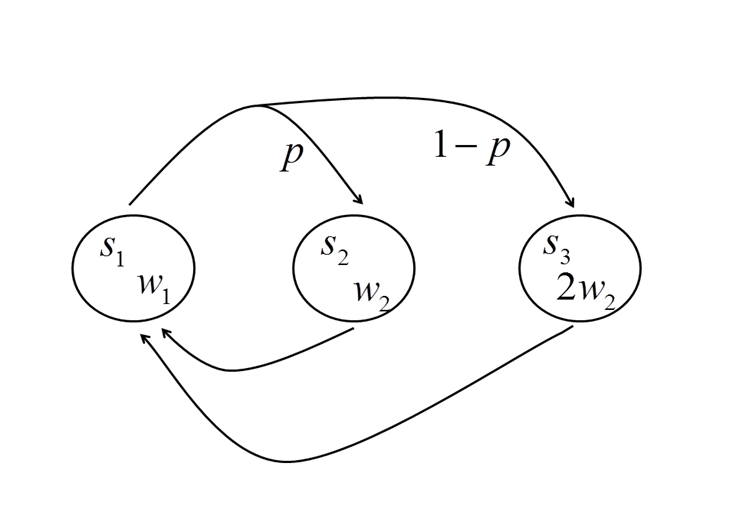
\includegraphics[width=0.6\textwidth]{hw8_a}
\end{center}

We consider a value function approximation $\tilde V(s) = {\phi _1}(s){w_1} + {\phi _2}(s){w_2}$, given explicitly as $\tilde V = {\left( {{w_1},{w_2},2{w_2}} \right)^ \top }$, and we let $w = {\left( {{w_1},{w_2}} \right)^ \top }$ denote the weight vector.

\begin{enumerate}
\setcounter{enumi}{1}
  \item What are the features $\phi (s)$ in this representation?
  \item Write down the Bellman operator ${T^\pi }$ explicitly. Write down${T^\pi }\tilde V$ .
  \item What is the stationary distribution?
  \item Write down the projection operator $\Pi $ explicitly, for $\epsilon = \left( \frac{1}{2},\frac{1}{4},\frac{1}{4}\right)$.
  \item Write an explicit expression for $\tilde V' \doteq \Pi {T^\pi }\tilde V$ in terms of $w$: the weight vector of $\tilde V$. Let $w' = {\left( {{w_1}',{w_2}'} \right)^ \top }$ denote the weights of $\tilde V'$. Write $w'$ as a function of $w$ .
  \item Show that iteratively applying $\Pi {T^\pi }$to $\tilde V$ may diverge for certain values of $p$.
\end{enumerate}
\end{exercise}

\begin{exercise}[\textbf{SARSA with function approximation}]
In this question we will implement a reinforcement learning algorithm in a continuous domain using function approximation.

Recall the tabular SARSA algorithm (Section \ref{ss:Q_eval}). We now present an extension of SARSA to the function approximation setting.
Assume that we are given a set of state-action features $\phi(s,a)\in \mathbb R^k$. We propose to approximate ${Q^\pi }(s,a)$ as a linear combination of these features:
$${\tilde Q^\pi }(s,a) = \mathop \sum \limits_{i = 1}^k {\phi _i}(s,a){w_i} \equiv \phi {(s,a)^ \top }w.$$
Our goal is to find the weight vector  $w \in \mathbb R^k$.

In the SARSA algorithm, at each stage we observe $\left( {{s_t},{a_t},{r_t},{s_{t + 1}},{a_{t + 1}}} \right)$, simulated on-policy (i.e., by simulating the policy $\pi $) and update $w$ by
\begin{align*}
w: &= w + {\beta _t}{\delta _t}\phi ({s_t},{a_t})\\
{\delta _t} &\buildrel \Delta \over = r({s_t}) + \gamma \phi {({s_{t + 1}},{a_{t + 1}})^ \top }w - \phi {({s_t},{a_t})^ \top }w
\end{align*}
where ${\beta _t}$ is a suitable step-size, and $\gamma $ is the discount factor.
\begin{enumerate}
  \item Explain the intuition for this update. You may use the TD(0) algorithm learned in class.
\end{enumerate}

Policy improvement in SARSA is achieved by choosing the policy $\pi $ as the  $\epsilon$-greedy policy with respect to the current $w$, that is, at time $t$ the state is ${x_t}$ and the action ${a_t}$ is selected according to
$${a_t} = \left\{ {\begin{array}{*{20}{c}}
{random}&{w.p.\,\,\,\epsilon}\\
{\arg {{\max }_a}\left( {\phi {{({s_t},a)}^ \top }w} \right)}&{w.p.\,\,1-\epsilon}
\end{array}} \right..$$

\begin{enumerate}
\setcounter{enumi}{1}
  \item Explain why the SARSA algorithm is expected to gradually improve performance.
\end{enumerate}

We will now implement SARSA on a popular RL benchmark - \emph{the mountain car}.
\begin{center}
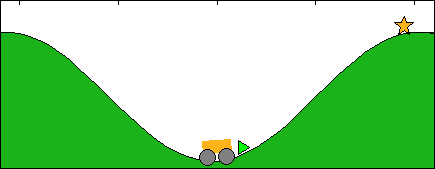
\includegraphics[width=0.6\textwidth]{hw8_b}
\end{center}

In the Mountain Car problem (see figure), an under-powered car must drive up a steep hill. Since gravity is stronger than the car's engine, even at full throttle, the car cannot simply accelerate up the steep slope. The car is situated in a valley and must learn to leverage potential energy by first driving up the left hill before gaining enough momentum to make it to the goal at the top of the right hill.

The state space is two-dimensional, and consists of the position $p \in \left[ { - 1.2,0.6} \right]$ and velocity $v \in \left[ { - 0.07,0.07} \right]$. There are 3 actions: $a =  - 1$ (accelerate left), $a = 0$ (don't accelerate), and $a = 1$ (accelerate right).

The simulation runs in episodes. At the beginning of an episode the initial state is ${p_0}\sim Uniform\left[ { - 0.5,0.2} \right]$, ${v_0}\sim Uniform\left[ { - 0.02,0.02} \right]$. If the car reaches the right hilltop: $p > 0.5$, the episode ends, and a reward $r = 5$ is received. At every other step the reward is $r =  - 1$. The maximum episode length is 500 steps.

The Matlab function \texttt{mountainCarSim(p, v, u)} (available at the course webpage) takes the current state and action and returns the next state of the car.

As function approximation, we will use grid-tiles. For each action $a$, we discretize the state space into $n$ non-overlapping tiles of size ${\Delta _p} = 0.1,{\Delta _v} = 0.01$ (see figure), and we label the tiles $\psi _1^a, \ldots ,\psi _n^a$.
\begin{center}
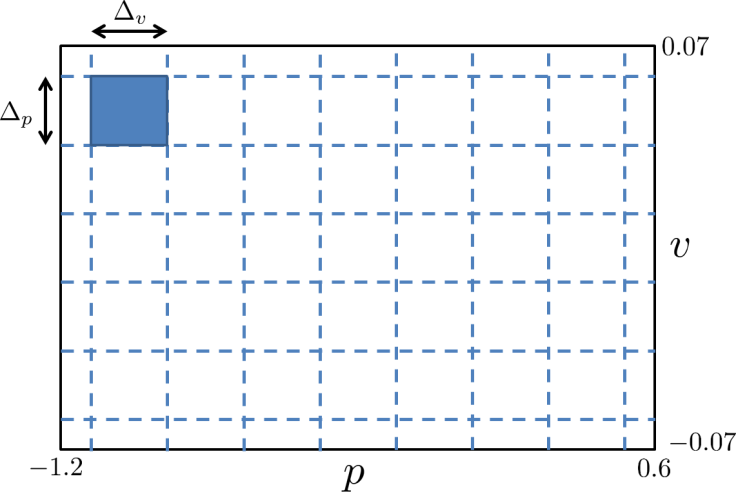
\includegraphics[width=0.6\textwidth]{hw8_c}
\end{center}

Define binary \textbf{state-features} $\phi(s)\in \mathbb R^n$  by:
\[{\phi _i}(s) = \left\{ {\begin{array}{*{20}{c}}
1&{s \in {\psi _i}\,}\\
0&{else}
\end{array}} \right.,\]
and binary \textbf{state-action-features} $\phi(s,a)\in \mathbb R^k$  where $k = 3n$,  by:
\[\begin{array}{l}
\phi (s, - 1) = \left\{ {\phi (s),2n\,\,{\rm{zeros}}} \right\}\\
\phi (s,0) = \left\{ {n\,\,{\rm{zeros}},\phi (s),n\,\,{\rm{zeros}}} \right\}\\
\phi (s,1) = \left\{ {2n\,\,{\rm{zeros}},\phi (s)} \right\}
\end{array}.\]

\begin{enumerate}
\setcounter{enumi}{2}
  \item Run the SARSA algorithm in this domain. Generate the following plots, and write a proper explanation for each plot.
  \begin{enumerate}
    \item Total reward (in episode) vs. episode
    \item Goal was reached / not reached vs. episode
    \item ${L_2}$ Norm of the weights $w$ vs. episode
    \item Trajectory of car ($p$ vs. time) for the greedy policy starting from $\left( {0,0} \right)$, every 100 episodes of learning.
    \item Final value function and policy after learning.
  \end{enumerate}
\end{enumerate}

You may use the following learning parameters for the algorithm:
\begin{itemize}
  \item Step size: ${\beta _t} = \frac{{100}}{{1000 + {\rm{episode count}}}}$
  \item Exploration: $\epsilon = 0.1$
  \item Discount: $\gamma  = 0.95$
  \item Total number of learning episodes: $500 - 1000$
  \item Initial weights: zeros.
\end{itemize}

\paragraph{Bonus:} Improve the learning algorithm using either:
\begin{itemize}
  \item Different features - you may try:
  \begin{itemize}
    \item Overlapping tiles (sometime called CMACs) (\url{http://webdocs.cs.ualberta.ca/~sutton/book/ebook/node88.html#SECTION04232000000000000000})
    \item Radial Basis Functions (\url{http://en.wikipedia.org/wiki/Radial_basis_function})
    \item Fourier / polynomials (\url{http://irl.cs.duke.edu/fb.php})
  \end{itemize}
  \item Different algorithm - you may try:
  \begin{itemize}
    \item SARSA($\lambda $) e.g., \url{http://webdocs.cs.ualberta.ca/~sutton/book/ebook/node89.html}
    \item Q($\lambda $) e.g., \url{http://webdocs.cs.ualberta.ca/~sutton/book/ebook/node89.html}
  \end{itemize}
  \item Any other idea that you like
\end{itemize}
Evidence that your method improves performance in some sense (learning rate/ final performance/ robustness to parameter changes/ etc.) will be rewarded with bonus points.
\end{exercise} 

\chapter{Policy Gradient Methods}
Recall that Reinforcement Learning is concerned with learning optimal control policies by interacting with the environment. So far, we have focused on learning methods that rely on learning the value function, from which the optimal policy can be inferred.
Policy gradient methods take a different approach. Here a set of \textbf{policies} is directly parameterized by a continuous set of parameters, which are then optimized online. The basic algorithms use online gradient descent, hence achieve only local optimality in the parameter space.
% To allow efficient learning, the parameter vector should be of a reasonably low dimension. 
This also means that the set of possible policies is restricted, and might require a fair amount of prior knowledge for its effective definition. On the other hand, the restriction to a given set of policies simplifies the treatment of various aspects of the RL problem such as large or continuous state and action spaces. For these reasons, policy gradient methods are finding many applications in the area of robot learning.
Policy Gradient algorithms belong to a larger class of Policy Search algorithms. An extensive survey can be found in:
\begin{itemize}
  \item M. Deisenroth, G. Neumann and J. Peters, "A Survey on Policy Search for Robotics," Foundations and Trends in Robotics, Vol. 2, 2011, pp. 1-142.
\end{itemize}
%
%Contents:
%13.1  Problem Description
%13.2  Finite Difference Methods
%13.3  Likelihood Ratio Methods

\section{Problem Description}

We consider the standard MDP model in discrete time, with states  ${x_t} \in X$, actions ${u_t} \in U$, transition kernel $\{ p(x'|x,u)\} $ , rewards  ${R_t} = {r_t}({x_t},{u_t})$, and policies $\pi  \in \Pi $.

For concreteness, we consider an episodic (finite horizon) problem with the total return criterion, which is to be maximized:
\[{J^\pi } = {\mathbb E^{\pi ,{x_0}}}\left(\sum\limits_{t = 0}^T {{R_t}} \right).\]
Here ${x_0}$ is a given initial state. We may allow the final time $T$ to depend on the state (as in the Stochastic Shortest Path problem), as long as it is bounded.

We next assume that we are given parameterized set of policies: $\{ {\pi _\theta },\,\theta  \in \Theta \} $, where $\theta $ is an $I$-dimensional parameter vector. We also refer to this set as a policy representation. The representation is often application-specific and should take into account prior knowledge on the problem.

We assume the following:
\begin{itemize}
  \item The actions set $U$ is continuous - typically a subset of $\mathbb R^l$.
If the original action set is finite, we extend it to a continuous set by considering  random (mixed) actions.
  \item The parameter set $\Theta $ is a continuous subset of $\mathbb R^I$.
  \item The policy set $\{ {\pi _\theta },\,\theta  \in \Theta \} $ is smooth in $\theta $. In particular, assuming each ${\pi _\theta }$ is a stationary policy,  ${\pi _\theta }(s)$ is a continuous function of $\theta $ for each state $s$.
\end{itemize}

\paragraph{Policy representation:} Some common generic representations include:
\begin{itemize}
  \item Linear policies:
                                      $$u = {\pi _\theta }(x) = {\theta ^T}\phi (x),$$
where $\phi (x)$ is a suitable set of basis functions (or  feature vectors).
  \item Radial Basis Function Networks:
             $${\pi _\theta }(x) = {w^T}\phi (x),  \textrm{ with }  {\phi _i}(x) = \exp ( - {\textstyle{1 \over 2}}{(x - {\mu _i})^T}{D_i}(x - {\mu _i})),$$
where ${D_i}$ is typically a diagonal matrix. The vector $\theta $ of tunable parameters includes $w$ (the linear parameters), and possibly $({\mu _i})$ and $({D_i})$ (nonlinear parameters).
  \item Neural Networks. For example, a Multi-Layer Perceptron (MLP):
  $$
    {\pi _\theta }(x) = \psi(b_2 + w_2^T \psi(b_1 + {w_1^T}\phi (x))),
  $$
  where $\psi$ is a non-linear activation function (e.g., $\tanh$ or sigmoid) and the vector $\theta$ includes the weight and the bias terms ($w_1,w_2,b_1,b_2$) in the neural network. This can be seen as a generalization of the linear policy to include non-linearities.
  \item Logistic (a.k.a. softmax) functions: For a discrete (finite) action space, one can use the Boltzman-like probabilities
                           $${\pi _\theta }(u|x) = \exp (w_u^T\phi (x))/\sum\nolimits_{u'} {\exp (w_{u'}^T\phi (x)} ),$$
where  $\theta  = {({w_u})_{u \in U}}$. It is convenient to designate one of the actions as 'anchor', with ${w_u} = 0$.
\item Stochastic policies: in certain cases a stochastic policy is required for sufficient exploration of the system. This is typically modelled by adding noise to a deterministic policy. For example, in a linear policy with Gaussian noise:
$$
P(u|x) = {\pi _\theta }(u|x) \sim \mathcal{N}\left( {w ^T}\phi (x), \sigma \right),
$$
where the parameter vector $\theta$ contains $w$ and the covariance matrix $\sigma$.
\end{itemize}

In robotics, a parameterized path is often described through a parameterized dynamical system, the output of which is used as a reference input to a feedback controller.

\paragraph{Gradient Updates:}  Plugging in the parameter-dependent policy ${\pi _\theta }$ in ${J^\pi }$,  we obtain the parameter-dependent return function:
\[J(\theta ) = {J^{{\pi _\theta }}}.\]

We wish to find a parameter $\theta $ that maximizes $J(\theta )$, at least locally. We discuss two high-level approaches for this task.

\section{Search in Parameter Space}
In this approach, the problem is viewed as a black-box optimization of the function $J(\theta )$.
Black-box optimization (a.k.a. derivative free optimization) refers to optimization of an objective function through a black-box interface: the algorithm may only query the function $J(\theta )$ for a point $\theta$; gradient information or the explicit form of $J(\theta)$ are not known. 

In our setting, for each given value of the parameter vector $\theta $, we can simulate or operate the system with control policy ${\pi _\theta }$ and measure the return  $\hat J(\theta ) = \sum\nolimits_{t = 0}^T {{R_t}} $, which gives a estimate of the expected return $J(\theta )$. We note that for stochastic systems or policies, this estimate will be noisy.

Note: The search in parameter space approach ignores the structure of our problem, namely, that trajectories are the result of rolling out a policy in an MDP. Only the mapping between $\theta$ and the resulting cumulative reward is considered.

Many black-box optimization algorithms have been proposed in the literature. We describe several that have been popular in RL literature.

\subsection{Gradient Approximation}

These methods use function evaluations of $J(\theta )$ to approximate the gradient ${\nabla _\theta }J(\theta )$.
Given the gradient, we may consider a gradient ascent scheme, of the form
\begin{equation}\label{eq:grad_ascent_scheme}
{\theta _{k + 1}} = {\theta _k} + {\alpha _k}\,{\nabla _\theta }J({\theta _k}).
\end{equation}
Here  $({\alpha _k})$ is the gain (or learning rate) sequence, and
\[{\nabla _\theta }J(\theta ) = \frac{{\partial J(\theta )}}{{\partial \theta }}\]
is the gradient of the return function with respect to $\theta $.

It remains of course to determine how to compute the required gradient. We next outline two options.

Note: Whenever required, we assume without further mention that $J(\theta )$ is continuously differentiable, and that the expectation and derivative in its definition can be interchanged.

\subsubsection*{Finite Difference Methods}
Finite difference methods are among the most common and straightforward methods for estimating the gradient in a variety of applications.

Suppose that, for each given value of the parameter vector $\theta $, we can simulate or operate the system with control policy ${\pi _\theta }$ and measure the return  $\hat J(\theta ) = \sum\nolimits_{t = 0}^T {{R_t}} $, which gives a estimate of the expected return $J(\theta )$. We note that this estimate will be noisy when either the policy or the system contain random moves.

\paragraph{Component-wise gradient estimates:} We can now obtain a noisy estimate of each component of the gradient vector using a finite difference of the form:
\[\frac{{\partial J(\theta )}}{{\partial {\theta _i}}} \approx \frac{{\hat J(\theta  + \delta {e_i}) - \hat J(\theta )}}{\delta },\]
or, preferably, the symmetric difference
  \[\frac{{\partial J(\theta )}}{{\partial {\theta _i}}} \approx \frac{{\hat J(\theta  + \delta {e_i}) - \hat J(\theta  - \delta {e_i})}}{{2\delta }}.\]
\paragraph{Note:}
\begin{itemize}
  \item Since the estimates $\hat J$ are typically noisy, repeated trials and averaging of several such differences are needed to reduce the estimation error. However, one can also use the noisy estimates with a low gain in the gradient ascent scheme, which has a similar averaging effect.
  \item The choice of the step size $\delta $ is crucial, as it controls the tradeoff between the relative noise level and the non-linearity of $J(\theta )$. We will not get into this issue here.
  \item A useful method to reduce the variance of the above difference is to use coupled random simulation, meaning that the random variables that govern the random choices in the simulation (or action choices) are drawn only once, and used for both estimates $\hat J(\theta  + \delta {e_i})$ and $\hat J(\theta  - \delta {e_i})$. These and other variance reduction methods are standard tools in the area of Monte-Carlo simulation.
\end{itemize}

\paragraph{Least-squared gradient estimates:}  Suppose we simulates/operate the system with a set of parameters ${\theta ^{[k]}} = \theta  + \Delta {\theta ^{[k]}}$, $1 \le k \le K$, to obtain a corresponding set of reward estimates ${\hat J^{[k]}} = \hat J(\theta  + \Delta {\theta ^{[k]}})$.

We can now use the linear relations
\begin{equation}\label{eq:LS_grad}
    \hat J(\theta  + \Delta {\theta ^{[k]}}) \approx J(\theta ) + \Delta {\theta ^{[k]}} \cdot \nabla J(\theta )
\end{equation}
to obtain a least-squares estimate of $\nabla J(\theta )$. For example, if an estimate $\hat J(\theta )$ is pre-computed, the relation
\[\Delta {J^{[k]}} \buildrel \Delta \over = \hat J(\theta  + \Delta {\theta ^{[k]}}) - \hat J(\theta ) \approx \Delta {\theta ^{[k]}} \cdot \nabla J(\theta )\]
leads to the LS estimate
\[\hat \nabla J(\theta ) = {({\bf{\Delta }}{{\bf{\Theta }}^T}{\bf{\Delta \Theta }})^{ - 1}}{\bf{\Delta }}{{\bf{\Theta }}^T}{\bf{\Delta J}},\]
where ${\bf{\Delta \Theta }} = {[\Delta {\theta ^{[1]}}, \ldots ,\Delta {\theta ^{[K]}}]^T}$, and ${\bf{\Delta J}} = {[\Delta {J^{[1]}}, \ldots ,\Delta {J^{[K]}}]^T}$.  (Note that we consider here $\Delta {\theta ^{[k]}}$ as a column vector, so that ${\bf{\Delta \Theta }}$ is a $K \times I$ matrix).

If $\hat J(\theta )$ is not given in advance, we can use directly the relations from \eqref{eq:LS_grad} in matrix form,
\[{\bf{\hat J}} \buildrel \Delta \over = \left[ {\begin{array}{*{20}{c}}
{{{\hat J}^{[1]}}}\\
 \vdots \\
{{{\hat J}^{[K]}}}
\end{array}} \right] \approx M\left[ {\begin{array}{*{20}{c}}
{J(\theta )}\\
{\nabla J(\theta )}
\end{array}} \right],\quad \quad M = [{\bf{1}},{\bf{\Delta \Theta }}]\]
to obtain the joint estimate ${({M^T}M)^{ - 1}}M\,{\bf{\hat J}}$ for $J(\theta )$ and $\nabla J(\theta )$.

\section{Population Based Methods}

This family of methods maintain a distribution over the parameter vector $\theta$, and use function evaluations to `narrow in' the distribution on an optimal choice. Assume that we have a parametrized distribution over the policy parameters $P_\phi(\theta)$. Note the distinction between the policy parameters $\theta$ and the parameters $\phi$ for the distribution of $\theta$ values.

For example, $P_\phi(\theta)$ can be a multivariate Gaussian, where $\phi$ encodes the mean and covariance of the Gaussian. 

\paragraph{Cross Entropy Method (CEM)}
This method updates $\phi$ iteratively according to the following scheme:
\begin{enumerate}
    \item Given current parameter $\phi_i$, sample $N$ population members
    $$
    \theta_k \sim P_{\phi_i}(\theta), \quad k=1,\dots,N.
    $$
    \item For each $k$, simulate the system with ${\pi_{\theta_k} }$ and measure the return $J(\theta_k)$.
    \item Let $K^*$ denote a set of the $p$\% top performing parameters
    \item Improve the parameter: 
    \begin{equation*}
    \phi_{i+1} = \argmax_\phi \sum_{k \in K^*} \log P_{\phi}(\theta_k). 
    \tag{$\star$}
    \end{equation*}
\end{enumerate}
The intuition here is that by refitting the distribution $P_\phi$ to the top performing parameters in the population, we are iteratively improving the distribution.

Note that other forms of the improvement step ($\star$) have been proposed in the literature. For example, in Reward Weighted Regression (RWR) the parameters are updated according to $$\phi_{i+1} = \argmax_\phi \sum_{k \in 1,\dots,N} J(\theta_k)\log P_{\phi}(\theta_k).$$

\section{Likelihood Ratio Methods}
Likelihood ratio-based methods allow to obtain a (noisy) estimate of the reward gradient from a \textbf{single} trial. The approach is again standard in the Monte-Carlo simulation area, where it is also known as the Score Function methods. Its first use in the controlled process (or RL) context is known as the REINFORCE algorithm. Interestingly, the RL formulation of this method can exploit the MDP structure of the problem, by using dynamic programming ideas to reduce variance in the estimation. 

Let ${\bf{\tau }} = ({x_0},{u_0}, \ldots ,{x_T})$ denote the process history, or sample path, of a single run of our episodic problem.  For simplicity we consider here a discrete model (finite state and action sets). Let ${p_\theta }({\bf{\tau }})$ denote the probability mass function induced on the process by the policy ${\pi _\theta }$. That is, assuming ${\pi _\theta }$ is a Markov policy,
\[{p_\theta }({\bf{\tau }}) = p({x_0})\prod\limits_{t = 0}^{T - 1} {{\pi _\theta }({u_t}|{x_t})p({x_{t + 1}}|{x_t},{u_t})}. \]
Denote $R({\bf{\tau }}) = \sum\nolimits_{t = 0}^{T - 1} {r({x_t},{u_t}) + {r_T}({x_T})} $, so that
\[J(\theta ) = {\mathbb E^\theta }(R({\bf{\tau }})) = \sum\nolimits_{\bf{\tau }} {R({\bf{\tau }}){p_\theta }({\bf{\tau }})\,} .\]
Observe now that${\nabla _\theta }{p_\theta }({\bf{\tau }}) = {p_\theta }({\bf{\tau }})\,{\nabla _\theta }\log {p_\theta }({\bf{\tau }})$. Therefore, assuming that the expectation and derivative can be interchanged,
\begin{align*}
\nabla J(\theta ) &= \sum\nolimits_{\bf{\tau }} {R({\bf{\tau }}){\nabla _\theta }{p_\theta }({\bf{\tau }})} \\
 &= \sum\nolimits_{\bf{\tau }} {[R({\bf{\tau }}){\nabla _\theta }\log {p_\theta }({\bf{\tau }})]\,{p_\theta }({\bf{\tau }})} \\
 &= {\mathbb E^\theta }\left( {R({\bf{\tau }}){\nabla _\theta }\log {p_\theta }({\bf{\tau }})} \right).
\end{align*}
Furthermore, observing the above expression for ${p_\theta }({\bf{\tau }})$,
\[{\nabla _\theta }\log {p_\theta }({\bf{\tau }}) = \sum\limits_{t = 0}^{T - 1} {{\nabla _\theta }\log {\pi _\theta }({u_t}|{x_t})} .\]
Importantly, the latter expression depends only on the derivative of the control policy, which is known to us, and not on the (unknown) process dynamics and reward function.

We can now obtain an unbiased estimate of $\nabla J(\theta )$ as follows:
\begin{itemize}
  \item Simulate/implement a single episode ("rollout") of the controlled system with policy ${\pi _\theta }$.
  \item Compute $R({\bf{\tau }})$ as $R({\bf{\tau }}) = \sum\nolimits_{t = 0}^{T - 1} {r({x_t},{u_t}) + {r_T}({x_T})} $, or directly using the observed rewards $R({\bf{\tau }}) \buildrel \Delta \over = \sum\nolimits_{t = 0}^T {{R_t}} $.
  \item Compute   $\hat \nabla J(\theta ) = R({\bf{\tau }})\sum\limits_{t = 0}^{T - 1} {{\nabla _\theta }\log {\pi _\theta }({u_t}|{x_t})} $
This is typically a noisy estimate, which can of course be improved by averaging over repeated trials.
\end{itemize}

\subsubsection{Illustrative Example}

Consider the bandit setting, where the MDP has only a single state and the horizon is $T=1$. The policy and reward are given as follows:
\begin{equation*}
    \begin{split}
        r(u) &= u, \\
        \pi_\theta(u) &= \frac{1}{\sqrt{2 \pi \sigma^2}} \exp (- \frac{(u - \theta)^2}{2 \sigma^2}).
    \end{split}
\end{equation*}
We have that $J(\theta) = \mathbb{E}[u] = \theta$, and thus $\nabla_\theta J(\theta) = 1.$
Using the policy gradient formula, we calculate:
\begin{equation*}
    \begin{split}
        \nabla_\theta \log \pi_\theta(u) &= \frac{u - \theta}{\sigma^2}, \\
        \nabla_\theta J(\theta) &= \mathbb{E} \left[\frac{u(u - \theta)}{\sigma^2}\right] \\
        &= \frac{1}{\sigma^2} (\mathbb{E} [u^2] - (\mathbb{E} [u])^2) = 1.
    \end{split}
\end{equation*}
Note the intuitive interpretation of the policy gradient here: we average the change to the mean action $u-\theta$ and the reward it produces $r(u)=u$. In this case, actions above the mean lead to higher reward, thereby `pushing' the mean action $\theta$ to increase. Also note the relation to the reward-weighted regression expression above.

\subsection{Variance Reduction}
We now provide a generalization of the policy gradient. We will consider an episodic MDP setting, and assume that for every policy parameter $\theta$, an absorbing state is reached w.p.~1. We can therefore replace the finite horizon return with an infinite sum ${J^\pi } = {\mathbb E^{\pi ,{x_0}}} \left(\sum\limits_{t = 0}^\infty {{R_t}} \right)$. We also recall the value and action value functions $V^\pi(x)$ and $Q^\pi(x,u)$. 
\begin{proposition}\label{prop:pg_control_variates}
The policy gradient can be written as:
\begin{equation*}
    \nabla_\theta J(\theta) = {\mathbb E^\theta }\left( \sum_{t=0}^\infty \Psi_t {{\nabla _\theta }\log {\pi _\theta }({u_t}|{x_t})} \right),
\end{equation*}
where $\Psi_t$ can be either one of the following terms:
\begin{enumerate}
    \item Total reward, $\sum_{t=0}^\infty r(x_t,u_t) - b(x_t)$, where $b$ is a state-dependent baseline
    \item Future reward following action $u_t$, $\sum_{t'=t}^\infty r(x_t,u_t) - b(x_t)$
    \item State-action value function, $Q^\pi(x_t,u_t)$
    \item Advantage function, $Q^\pi(x_t,u_t) - V^\pi(x_t)$
    \item Temporal difference, $r(x_t,u_t) + V^\pi(x_{t+1})- V^\pi(x_t)$
\end{enumerate}
\end{proposition}

All the above formulations are unbiased estimates of the policy gradient. However, they differ in their variance, and variance reduction plays an important role in practical applications\footnote{In the simulation literature, the technique of changing the variance of the estimate by adding terms that do not change its bias is known as \textit{control variates}.}. Let illustrate this in the previous bandit example.

\subsubsection{Illustrative Example (cont'd)}
Consider the previous bandit setting, where we recall that
$        r(u) = u, \quad
        \pi_\theta(u) = \frac{1}{\sqrt{2 \pi \sigma^2}} \exp (- \frac{(u - \theta)^2}{2 \sigma^2}).$
Find a fixed baseline $b$ that minimizes the variance of the policy gradient estimate.

The policy gradient formula in this case is:
\begin{equation*}
        \nabla_\theta J(\theta) = \mathbb{E} \left[\frac{(u-b)(u - \theta)}{\sigma^2}\right] = 1, 
\end{equation*}
and we can calculate the variance
\begin{equation*}
\begin{split}
        \frac{1}{\sigma^4}\textrm{Var}\left[(u-b)(u - \theta)\right]  
        &=\frac{1}{\sigma^4}\mathbb{E}\left[\left((u-b)(u - \theta)\right)^2 - 1\right] \\
        &=\frac{1}{\sigma^4}\mathbb{E}\left[\left((u-\theta)(u - \theta) + (\theta-b)(u - \theta)\right)^2 - 1\right] \\
        &=\frac{1}{\sigma^4}\mathbb{E}\left[(u-\theta)^4 + 2(\theta-b)(u - \theta)^3 + (\theta-b)^2(u - \theta)^2 - 1\right] \\
        &=\frac{1}{\sigma^4}\mathbb{E}\left[(u-\theta)^4 + (\theta-b)^2(u - \theta)^2 - 1\right],
\end{split}
\end{equation*}
which is minimized for $b=\theta$.

\textbf{Note 1}: The average reward, state-action value function, and advantage function baselines are commonly used in practice. While in our illustrative example the average reward was optimal, in general it is not necessarily so. An in-depth discussion of this topic can be found in:  
\begin{itemize}
  \item Greensmith, E., Bartlett, P.L. and Baxter, J., 2004. Variance reduction techniques for gradient estimates in reinforcement learning. Journal of Machine Learning Research, 5(Nov), pp.1471-1530.
\end{itemize}
Nevertheless, these baselines often lead to significant performance gains in practice.

\textbf{Note 2}: Typically, the value functions $V^\pi$ and $Q^\pi$ will not be known, and will have to be estimated along with the policy gradient using TD methods or regression. An important question here is how the error in value function estimation affects the policy gradient bias. There exist special policy classes and function approximators that are said to be \textit{compatible}, where the value estimation error is orthogonal to the policy gradient bias. In general, however, this is not the case. 


\subsubsection{Proof of Proposition \ref{prop:pg_control_variates}}
\begin{proof}
We will start by establishing a useful property. 
Let $p_\theta(z)$ be some parametrized distribution. Differentiating $\sum\nolimits_{z } {{p_\theta }(z)}  = 1$  yields
\begin{equation}\label{eq:helper}
\sum\nolimits_{z} {(\nabla \log {p_\theta }({z})} ){p_\theta }({z}) = {\mathbb E^\theta }(\nabla \log {p_\theta }({z})) = 0.
\end{equation}

We can now observe that adding a state-dependent baseline to the policy gradient does not add bias:
\begin{equation*}
\begin{split}
{\mathbb E^\theta }\left( \sum_{t=0}^\infty b(x_t) {{\nabla _\theta }\log {\pi _\theta }({u_t}|{x_t})} \right) &= \sum_{t=0}^\infty {\mathbb E^\theta }\left[ b(x_t) {{\nabla _\theta }\log {\pi _\theta }({u_t}|{x_t})} \right] \\ 
&= \sum_{t=0}^\infty {\mathbb E^\theta }\left[ {\mathbb E^\theta }\left[ \left. b(x_t) {{\nabla _\theta }\log {\pi _\theta }({u_t}|{x_t})} \right| x_t \right]\right] \\ 
&= \sum_{t=0}^\infty {\mathbb E^\theta }\left[ b(x_t) {\mathbb E^\theta }\left[ \left. {{\nabla _\theta }\log {\pi _\theta }({u_t}|{x_t})} \right| x_t \right]\right] \\ 
&= 0,
\end{split}
\end{equation*}
where the last equation follows from applying \eqref{eq:helper} to the inner expectation. Note that the justification for exchanging the expectation and infinite sum in the first equality is not straightforward. In this case it can be shown to hold by the Fubini theorem, using the assumption that every trajectory reaches a terminal state in a bounded time w.p.~1.

We continue to show the independence on past rewards. We have that
\begin{equation*}
\begin{split}
& {\mathbb E^\theta }\left[ \sum_{t=0}^\infty \sum_{t'=0}^{t-1} r(x_{t'},u_{t'}) {{\nabla _\theta }\log {\pi _\theta }({u_t}|{x_t})} \right] \\
&= \sum_{t=0}^\infty {\mathbb E^\theta }\left[ \sum_{t'=0}^{t-1} r(x_{t'},u_{t'}) {{\nabla _\theta }\log {\pi _\theta }({u_t}|{x_t})} \right] \\
&= \sum_{t=0}^\infty {\mathbb E^\theta }\left[ {\mathbb E^\theta }\left[ \left. \sum_{t'=0}^{t-1} r(x_{t'},u_{t'}) {{\nabla _\theta }\log {\pi _\theta }({u_t}|{x_t})} \right| x_0,u_0,\dots,x_t \right]\right] \\
&= \sum_{t=0}^\infty {\mathbb E^\theta }\left[ \sum_{t'=0}^{t-1} r(x_{t'},u_{t'}) {\mathbb E^\theta }\left[ \left. {{\nabla _\theta }\log {\pi _\theta }({u_t}|{x_t})} \right| x_0,u_0,\dots,x_t \right]\right] \\
&= \sum_{t=0}^\infty {\mathbb E^\theta }\left[ \sum_{t'=0}^{t-1} r(x_{t'},u_{t'}) {\mathbb E^\theta }\left[ \left. {{\nabla _\theta }\log {\pi _\theta }({u_t}|{x_t})} \right| x_t \right]\right] \\
&=0, 
\end{split}    
\end{equation*}
where in the second to last equality we used the Markov property, and in the last equality we again applied \eqref{eq:helper}. We have thus proved (1) and (2).

\textbf{Exercise 1:} where would this derivation fail for future rewards?
% Solution: the Markov property is required to obtain an expectation on P(u|x) which is the distribution of the policy, as required by \eqref{eq:helper}.

We continue to prove (3).
\begin{equation*}
\begin{split}
& {\mathbb E^\theta }\left[ \sum_{t=0}^\infty \sum_{t'=t}^{\infty} r(x_{t'},u_{t'}) {{\nabla _\theta }\log {\pi _\theta }({u_t}|{x_t})} \right] \\
& \sum_{t=0}^\infty {\mathbb E^\theta }\left[ \sum_{t'=t}^{\infty} r(x_{t'},u_{t'}) {{\nabla _\theta }\log {\pi _\theta }({u_t}|{x_t})} \right] \\
& \sum_{t=0}^\infty {\mathbb E^\theta }\left[ {\mathbb E^\theta }\left[ \left. \sum_{t'=t}^{\infty} r(x_{t'},u_{t'}) {{\nabla _\theta }\log {\pi _\theta }({u_t}|{x_t})}\right| x_t, u_t\right] \right] \\
& \sum_{t=0}^\infty {\mathbb E^\theta }\left[ {{\nabla _\theta }\log {\pi _\theta }({u_t}|{x_t})} {\mathbb E^\theta }\left[ \left. \sum_{t'=t}^{\infty} r(x_{t'},u_{t'}) \right| x_t, u_t\right] \right] \\
& \sum_{t=0}^\infty {\mathbb E^\theta }\left[ {{\nabla _\theta }\log {\pi _\theta }({u_t}|{x_t})} Q^\pi(x_t,u_t) \right]. \\
\end{split}    
\end{equation*}

\textbf{Exercise 2:} Prove (4) and (5).

\end{proof}

\subsection{Natural Policy Gradient}
In the gradient ascent scheme \eqref{eq:grad_ascent_scheme}, the idea is to take small steps that iteratively improve the policy. The question is, what is the best metric to define `small steps' in?
Taking a step $\eta$ in the gradient direction is equivalent to solving the following optimization problem:
\begin{equation}\label{eq:grad_descent_opt}
    \begin{split}
        \argmax_{\Delta \theta}&\quad \Delta \theta^\top \nabla J(\theta), \\
        s.t. &\quad \Delta \theta^\top \Delta \theta \leq \eta.
    \end{split}
\end{equation}
Thus, standard gradient ascent takes a small improvement step w.r.t.~a Euclidean distance in the parameter space. However, this scheme can be highly sensitive to the specific parametrization employed - it might be that a small change in parameters causes a very drastic change to the behavior of the policy. The natural gradient attempts to rectify this situation by replacing the Euclidean distance between two parameters $\theta $  and $\theta+\Delta\theta$ by the Kullback-Leibler distance\footnote{The Kullback–Leibler (KL) distance between two distributions $P,Q$ is defined as $D_{KL}(P||Q) = \sum_{x}P(x)\log \frac{P(x)}{Q(x)}$. It is a standard tool in information theory.} between the probability distributions ${p_\theta }({\bf{\tau }})$ and ${p_{\theta+\Delta\theta}}({\bf{\tau }})$ induced by these parameters. Using a Taylor expansion, the KL distance can be approximated as 
\begin{equation*}
    D_{KL}({p_\theta }({\bf{\tau }})||{p_{\theta+\Delta\theta}}({\bf{\tau }})) \approx \Delta \theta^\top F_\theta \Delta \theta,
\end{equation*}
where $F_\theta$ is the Fisher Information Matrix, $F_\theta = \sum_\tau p_\theta(\tau) \nabla \log p_\theta(\tau) \nabla \log p_\theta(\tau)^\top.$

Replacing the constraint in \eqref{eq:grad_descent_opt} with $\Delta \theta^\top F_\theta \Delta \theta \leq \eta$ leads to a modified gradient definition known as the Natural Gradient: :
\[{\nabla ^N}J(\theta ) = F_{\theta}^{ - 1}\nabla J(\theta ).\]
% where $\nabla J$ is the standard gradient, and $F(\theta )$ is the Fisher Information Matrix:
% \begin{align*}
% F(\theta ) &= \sum\nolimits_{\bf{\tau }} {{p_\theta }({\bf{\tau }})} (\nabla \log {p_\theta }({\bf{\tau }})){(\nabla \log {p_\theta }({\bf{\tau }}))^T}\\
%  &= {\mathbb E_{{\bf{\tau }} \sim {p_\theta }}}\left( {(\nabla \log {p_\theta }({\bf{\tau }})){{(\nabla \log {p_\theta }({\bf{\tau }}))}^T}} \right).
% \end{align*}
Note that the Fisher Information Matrix can be calculated by sampling, since $\log p_\theta(\tau)$ only requires knowing the policy (as in the policy gradient derivation above). 
Natural policy gradient schemes lead in general to faster and more robust convergence to the optimal policy.

% \paragraph{Variations and improvements:}
% \begin{enumerate}
%   \item Baseline variance reduction:  A somewhat more general estimate for $\nabla J(\theta )$ can be obtained by subtracting a constant from$R({\bf{\tau }})$, namely
%                                       \[\hat \nabla J(\theta ) = (R({\bf{\tau }}) - b)\sum\limits_{t = 0}^{T - 1} {{\nabla _\theta }\log {\pi _\theta }({u_t}|{x_t})} .\]
% This estimate remains unbiased, as differentiating $\sum\nolimits_{\bf{\tau }} {{p_\theta }({\bf{\tau }})}  = 1$  yields
%                               \[\sum\nolimits_{\bf{\tau }} {(\nabla \log {p_\theta }({\bf{\tau }})} ){p_\theta }({\bf{\tau }}) = {\mathbb E^\theta }(\nabla \log {p_\theta }({\bf{\tau }})) = 0.\]
% A proper choice of the constant $b$ can however significantly reduce the variance.  The optimal value of  $b$ can itself be estimated from the data.
%   \item Natural Gradients:  The gradient $\nabla J(\theta )$ is highly sensitive to the specific parametrization employed, even if the set of policies ${\{ {\pi _\theta }\} _{\theta  \in \Theta }}$ is the same.
% For example, replacing the component ${\theta_1}$ of the parameter vector by $\theta_1' = 10\,\theta_1$ changes the gradient direction.
% The natural gradient attempts to rectify this situation by replacing the Euclidean distance between two parameters $\theta $  and $\theta '$ by an appropriate distances between the probability distributions ${p_\theta }({\bf{\tau }})$ and ${p_{\theta '}}({\bf{\tau }})$ induced by these parameters. This leads a modified gradient definition known as the Natural Gradient: :
% \[{\nabla ^N}J(\theta ) = F{(\theta )^{ - 1}}\nabla J(\theta ),\]
% where $\nabla J$ is the standard gradient, and $F(\theta )$ is the Fisher Information Matrix:
% \begin{align*}
% F(\theta ) &= \sum\nolimits_{\bf{\tau }} {{p_\theta }({\bf{\tau }})} (\nabla \log {p_\theta }({\bf{\tau }})){(\nabla \log {p_\theta }({\bf{\tau }}))^T}\\
%  &= {\mathbb E_{{\bf{\tau }} \sim {p_\theta }}}\left( {(\nabla \log {p_\theta }({\bf{\tau }})){{(\nabla \log {p_\theta }({\bf{\tau }}))}^T}} \right).
% \end{align*}
% Natural policy gradient schemes have been developed which estimate the natural gradient by observing the system. These algorithms lead in general to faster and more robust convergence to the optimal policy.
%   \item Q-Function based gradient estimates:   In stationary problems (infinite horizon or SSP), the variance of the gradient estimates can be improved significantly by using a modified expression which involves the Q-function. This formulation is therefore the most commonly used.
% Consider an SSP problem, where T is the arrival time to some set of states. Let ${Q^{{\pi _\theta }}}(x,u)$ denote the Q-function under the stationary policy ${\pi _\theta }$.  Then the following holds (the proof will be discussed in the Tirgul):
% \[{\nabla _\theta }J(\theta ) = {\mathbb E^\theta }\sum\limits_{t = 0}^{T - 1} {({\nabla _\theta }\log {\pi _\theta }({u_t}|{x_t})){Q^{{\pi _\theta }}}({x_t},{u_t})} .\]
% This expression is known as the \emph{policy gradient theorem}. It can be used to estimate the gradient, by running in parallel an (independent) algorithm for estimating Q.
% \end{enumerate}




\bibliography{references}
\bibliographystyle{ieeetr}

\end{document}

